\documentclass[dosguias,openany]{tesisusach}
% La opción dosguias permite incluir profesor co-guía con \profesorco{}
% La clase está basada en la clase book, por lo que las opciones de esta son
% pasadas directamente. La opción openany es para evitar páginas en blanco
% entre capítulos y es una opción de la clase book, que es un requerimiento
% del repositorio central

% Acá van todos los paquetes necesarios, aunque la clase ed por sí requiere
% ya varios, como biblatex, caption, inputenc (con utf8), etc.
\usepackage{lipsum}
\usepackage{longtable}
\usepackage{booktabs}
\usepackage{array}
\usepackage{tabularx}
\usepackage{graphicx}
\usepackage{subcaption}
\usepackage{graphicx}
\usepackage{amsmath,amssymb}
\usepackage{rotating}
\usepackage{multirow}
\usepackage[table]{xcolor}
\usepackage[ruled,vlined,linesnumbered]{algorithm2e}

\newcolumntype{C}[1]{>{\centering\arraybackslash}p{#1}}
\providecommand{\Atwelve}{\ensuremath{\hat{A}_{12}}}

\title{Implementación de un algoritmo evolutivo basado en optimización esparsa multiobjetivo a gran escala para Redes Neuronales de Espigas}
\author{Nicolás Aguilera González}
% La fecha de la portada solo requiere el año
\date{\the\year}

\keywordsEs{Redes Neuronales de Espigas, Computación Neuromórfica, Neuroevolución, Optimización Multiobjetivo Esparsa a Gran Escala, Modelo de Izhikevich, Algoritmos Evolutivos, Frente de Pareto, Hipervolumen}
\keywordsEn{Spiking Neural Networks, Neuromorphic Computing, Neuroevolution, Large-Scale Sparse Multi-Objective Optimization, Izhikevich Model, Evolutionary Algorithms, Pareto Front, Hypervolume}

% Acá el texto está en minúscula solo para probar la versalita en la portada
%\universidad{universidad de santiago de chile}
% \subtitle{O la memoria, si es que es el caso\ldots}

\facultad{Facultad de Ingeniería}
\unidad{Departamento de Ingeniería Informática}
\profesor{Javier Baladron}
\profesorco{Manuel Villalobos}
\propuesta{Tesis para optar al título de Ingeniero Civil en Informática}
\ciudad{Santiago}
\pais{Chile}

% Por si hiciera falta reemplazar el logo de la portada,
% el comando \logo lo puede colocar
%\logo{
\includegraphics[scale=.25]{./images/LogoUsach2.png}}

% Archivo de referencias
\addbibresource{caps/referencias.bib}

\begin{document}
	\maketitle
	% ----------------------------------------------------------
	% ----------- PRIMERA PARTE --------------------------------
	% Temas preliminares: abstract, agradecimientos, 
	% dedicatorias...
	\frontmatter
	
	% Los resúmenes son "capítulos" en cuanto a formato, pero como deben aparecer
	% en páginas seguidas, hay dos opciones principales: se utilizan opciones como
	% oneside (todas las páginas son "páginas derechas") u openany (doble página),
	% pero los capítulos inician en cualquier página, o se omite el inicio en
	% cualquier página para el resumen. Estos comandos antes y después del resumen
	% logran eso
	%\makeatletter % convierte @ en letra, en vez de caracter especial
	%\@openrightfalse % anula empezar capítulo en página derecha

	\newpage
    Este trabajo se enmarca dentro del proyecto \textbf{Fondecyt Regular 1251455 NeuroMetaEvo: Integrating Metaheuristic Techniques with Neuroscience for Advanced Neuromorphic Algorithm Design}.

	
	\begin{resumenEs}
		Las Redes Neuronales de Espigas (SNN) son un paradigma de computación neuromórfica inspirado en el cerebro, donde la información se procesa mediante eventos discretos (espigas), lo que promete mayor eficiencia energética que las redes neuronales artificiales (ANN) convencionales. Sin embargo, su entrenamiento se ve limitado por la naturaleza no diferenciable de la función de disparo, que impide aplicar directamente \textit{Backpropagation}. Esta tesis aborda el problema mediante neuroevolución, empleando algoritmos evolutivos multiobjetivo esparsos a gran escala (SMOEA) que optimizan simultáneamente topología y pesos sinápticos de una SNN sin depender de gradientes, buscando equilibrar precisión de clasificación y esparsidad estructural.

		A partir de una taxonomía de SMOEAs, se seleccionaron dos algoritmos, S-NSGA-II y MOEA-CKF, migrados desde PlatEMO (MATLAB) a una implementación propia en C++, integrada con un simulador de SNN basado en el modelo de Izhikevich, validado en este trabajo con desempeño estadísticamente superior a ANNarchy y NEST. El sistema se evaluó en cuatro \textit{datasets} de clasificación binaria del repositorio UCI (Statlog Australian, Climate, Statlog German y Connectionist Bench Sonar), mediante 31 corridas pareadas por semilla y análisis estadístico del Hipervolumen (HV), los frentes de Pareto y la velocidad de convergencia.

		Los resultados muestran que S-NSGA-II y MOEA-CKF alcanzan un HV estadísticamente equivalente, con ventajas de S-NSGA-II en \textit{datasets} de menor dimensionalidad y de MOEA-CKF en el de mayor dimensionalidad, además de diferencias en tiempo de cómputo. Frente a la ANN (PlatEMO/MATLAB), esta superó a la SNN en HV y exactitud en las ocho combinaciones evaluadas, aunque la SNN resultó más esparsa. El análisis de conectividad reveló que, al no incorporar noción de topología, los operadores de dispersión generan una fracción relevante de soluciones estructuralmente incoherentes. Se concluye que el objetivo general se cumple parcialmente, con una plataforma funcional y validada estadísticamente, y líneas claras de trabajo futuro.
	\end{resumenEs}

	\begin{resumenEn}
		Spiking Neural Networks (SNNs) are a neuromorphic computing paradigm inspired by the brain, in which information is processed through discrete events (spikes), promising greater energy efficiency than conventional artificial neural networks (ANNs). However, their training is hindered by the non-differentiable nature of the spiking function, which prevents the direct application of \textit{Backpropagation}. This thesis addresses the problem through neuroevolution, using large-scale sparse multi-objective evolutionary algorithms (SMOEAs) that simultaneously optimize the topology and synaptic weights of an SNN without relying on gradients, seeking to balance classification accuracy and structural sparsity.

		Based on a taxonomy of SMOEAs, two algorithms, S-NSGA-II and MOEA-CKF, were selected and migrated from PlatEMO (MATLAB) to a custom C++ implementation, integrated with an SNN simulator based on the Izhikevich neuron model, validated in this work with statistically superior performance to ANNarchy and NEST. The system was evaluated on four binary classification datasets from the UCI repository (Statlog Australian, Climate, Statlog German, and Connectionist Bench Sonar), through 31 seed-paired runs and statistical analysis of Hypervolume (HV), the resulting Pareto fronts, and convergence speed.

		Results show that S-NSGA-II and MOEA-CKF achieve statistically equivalent HV, with S-NSGA-II performing better on lower-dimensionality datasets and MOEA-CKF on the highest-dimensionality one, along with systematic differences in computation time. Compared to its ANN counterpart (PlatEMO/MATLAB), the latter outperformed the SNN in HV and accuracy across all eight evaluated combinations, although the SNN proved sparser. Connectivity analysis further revealed that, lacking any notion of topology, the sparsity operators generate a substantial fraction of structurally incoherent solutions. It is concluded that the general objective was only partially met, with a functional, statistically validated platform and clear directions for future work.
	\end{resumenEn}
	%\@openrighttrue % restaura empezar capítulo en página derecha
	%\makeatother % restaura @ como carácter especial

	% Para una dedicatoria de una línea o dos
	% \dedicatoriaSimple{A Lilith, señora de los desposeídos}
	
	\begin{agradecimiento}
		Agradezco a todos quienes fueron parte no solamente de este trabajo sino a los que estuvieron en todo el camino recorrido hasta llegar aquí, a los que están y a los que ya no, a mi familia y mi pareja por siempre brindarme apoyo incondicional, y a mis amigos y compañeros por hacer de este camino, uno lleno de risas, de buenos y no tan buenos momentos, pero por sobre todo por estar y compartirme siempre un pedacito de ellos. A los buenos docentes que día a día se entregan en el aula, a los que no se rinden y tienen convicción de que una buena docencia es capaz de transformar desde adentro. A los conserjes del departamento por siempre recibirnos con una sonrisa y buena disposición para lo que fuera.

        A todos les agradezco y les puedo decir que al fin lo logré.
	\end{agradecimiento}

	% De acuerdo al formato, lo preliminar termina con las tablas
	% de contenido.
	\tableofcontents
	\newpage
	%% Indice de tablas
	\listoftables
	\newpage
	%% Indice de figuras
	\listoffigures
	\newpage
	% Acá puede ir cualquier índice adicional del trabajo hecho, como códigos, algoritmo, etc.

	% ----------------------------------------------------------
	% ----------- SEGUNDA PARTE --------------------------------
	% Los capítulos solo están de relleno como ejemplo con el paquete lipsum
	% Los contenidos de estos capítulos son típico código estándar de LaTeX
	\mainmatter
	% Archivo de ejemplo para colocar introducción
\chapter{Introducción}\label{cap:intro}

\section{Antecedentes y motivación}
En la última década, el aprendizaje profundo (Deep Learning) ha revolucionado la inteligencia artificial \cite{dean2022golden}, sin embargo, este avance ha conllevado un costo computacional y energético insostenible. Sin ir más lejos, un computador estándar que usa redes profundas para reconocer 1000 tipos de objetos diferentes, requiere alrededor de 250W \cite{roy2019spike}, necesitando un consumo energético superior a los 20W que necesita el cerebro humano para realizar simultáneamente tareas de razonamiento, reconocimiento y control \cite{roy2019spike}.

Frente a esto, la Computación Neuromórfica y las Redes Neuronales de Espigas (SNN) emergen como una alternativa eficiente, inspirada en el cerebro humano \cite{Schuman2022Opportunities}, donde la información no se procesa de forma continua, sino que se transmite mediante impulsos discretos, o espigas. A diferencia de las Redes Neuronales Artificiales (ANN), las SNN emulan la forma en que las neuronas del cerebro generan y responden a estos impulsos, operando de manera asíncrona y dispersa (event-driven), lo que teóricamente permite un consumo energético drásticamente menor \cite{Schuman2022Opportunities}. Esta escasez de actividad, parte de su procesamiento basado en eventos, las convierte en una opción más viable para sistemas con limitaciones de energía y recursos computacionales. Sin embargo, el despliegue masivo de SNNs enfrenta una barrera crítica: la dificultad de su entrenamiento.


\section{Descripción del problema}
Uno de los principales obstáculos técnicos para entrenar las SNN es que las funciones de activación de las neuronas no son diferenciables, lo que impide el uso directo del algoritmo de \textit{Backpropagation} (estándar en ANN) para su entrenamiento. Sin embargo, existen alternativas a este problema, como el uso de \textit{surrogate gradients}, que aunque efectivas, son computacionalmente costosas y biológicamente poco plausibles. Por otro lado, técnicas como STDP (Spike-Timing-Dependent Plasticity) a menudo no escalan bien para tareas complejas de clasificación. Existe, por tanto, la necesidad de métodos de entrenamiento que:

\begin{enumerate}
    \item No dependan de gradientes (diferenciabilidad).
    \item Aprovechen la naturaleza discreta de las SNN.
    \item Optimicen no solo los pesos sinápticos, sino también la arquitectura (topología) para crear redes eficientes.
\end{enumerate}

Se propone la siguiente pregunta de investigación: ¿cómo entrenar SNN sin depender de gradientes, aprovechando la naturaleza discreta de los spikes, modificando simultáneamente la estructura y los pesos de la red, para minimizar la cantidad de conexiones activas y el error en tareas de clasificación, equilibrando ambos objetivos sin sacrificar significativamente el rendimiento?

\section{Solución propuesta}
\subsection{Enfoques de solución}

En el contexto de la computación neuromórfica, el entrenamiento de Redes Neuronales de Espigas (SNN) presenta desafíos únicos debido a la naturaleza discreta y no diferenciable de los spikes. Para determinar la estrategia de entrenamiento más adecuada para este proyecto, se han considerando tres criterios:

\begin{enumerate}
    \item \textbf{Eficiencia Estructural (Sparsity):} capacidad intrínseca del método para generar topologías dispersas (menos conexiones) que reduzcan el consumo energético en la inferencia.
    \item \textbf{Exactitud (Accuracy):} capacidad del modelo para clasificar correctamente en benchmarks estándar.
    \item \textbf{Costo Computacional de Entrenamiento:} recursos de memoria y procesamiento requeridos para encontrar la solución óptima.
\end{enumerate}

Estos criterios permiten comparar los cinco enfoques que se presentan a continuación, basado en los resultados de la literatura y a partir de ello, seleccionar el más adecuado para el desarrollo de una solución al problema planteado. En la Tabla \ref{tab:enfoques-comp} se presenta una comparación entre los cinco enfoques, considerando los criterios antes mencionados.

\paragraph{Aprendizaje con gradientes sustitutos.} Los métodos de \textit{surrogate gradient} adaptan el \textit{Backpropagation} a SNN reemplazando la función de activación no diferenciable por una aproximación suave, permitiendo entrenar SNN profundas \cite{Schuman2022Opportunities}. Sin embargo, requieren almacenar la dinámica temporal de las neuronas, lo que incrementa el costo de memoria y cómputo \cite{Neftci2019SurrogateGradient}.

\paragraph{Mapeo de redes profundas pre-entrenadas.} Este enfoque convierte ANN en SNN ajustando pesos y umbrales, obteniendo buenos resultados en benchmarks como CIFAR-10 e ImageNet \cite{deng2021optimal}. Sin embargo, genera redes densas, lo que puede reducir la eficiencia de la red \cite{deng2021optimal}.

\paragraph{Neuroevolución.} Usa algoritmos evolutivos para optimizar arquitecturas y parámetros de redes neuronales, incluidas las SNN, sin requerir gradientes \cite{risi2025neuroevolution}. Es útil para diseñar topologías eficientes y enfrentar dinámicas no lineales. Sin embargo, la escalabilidad sigue siendo un reto \cite{Yue2025CNEA, Shen2024EvolutionarySNN}.

\paragraph{Computación de reservorio.} Utiliza SNN recurrentes no entrenadas para proyectar entradas a espacios de alta dimensión espacio-tiempo, facilitando el procesamiento de secuencias con un costo de entrenamiento bajo. Sin embargo, el desempeño depende del diseño del reservorio, y para tareas complejas se requieren reservorios grandes \cite{Duran2025CMOSSNNReservoir,Polydoros2015ReservoirComputing}.

\paragraph{Plasticidad dependiente del tiempo de disparo (STDP).} Es una regla de aprendizaje local que modifica los pesos sinápticos según la relación temporal entre los disparos neuronales. Aunque es eficiente en hardware neuromórfico, su rendimiento en tareas de clasificación es inferior a las técnicas supervisadas modernas \cite{Liu2021SSTDP, Schuman2022Opportunities}. 

\begin{table}[h]
    \centering
    \small
\caption{Comparación de enfoques de solución.}
\label{tab:enfoques-comp}
    \begin{tabular}{>{\centering\arraybackslash}p{0.15\linewidth}>{\centering\arraybackslash}p{0.25\linewidth}>{\centering\arraybackslash}p{0.25\linewidth}>{\centering\arraybackslash}p{0.25\linewidth}}\toprule
         \textbf{Enfoque}&  \textbf{Precisión (Clasificación)}& \textbf{Eficiencia Estructural (Sparsity/Topología)}& \textbf{ Costo de entrenamiento (Cómputo/Memoria)}\\\midrule
         \textbf{Surrogate Gradient}&  Muy Alta (Estado del Arte)& Baja (Suele operar sobre arquitecturas fijas y densas)&  Muy Alto (Requiere BPTT y almacenar historial temporal)\\
         \textbf{Neuroevolución}&  Media / Alta& Muy Alta (Permite optimizar topología explícitamente)&  Alto (Requiere evaluar poblaciones completas)\\
        \textbf{ Mapeo ANN-a-SNN}&  Alta (Heredada de ANN)& Baja (Hereda la densidad de la ANN, alta latencia)&  Medio (Entrenamiento estándar de ANN + Conversión)\\
         \textbf{Reservoir Computing}&  Baja / Media& Nula (Reservorio aleatorio, generalmente grande y redundante)&  Bajo (Solo se entrena la capa de lectura)\\
         \textbf{STDP}&  Baja (En tareas complejas)& Media (Induce sparsity biológica, pero difícil de controlar)&  Bajo (Regla local, sin gradientes globales)\\\bottomrule
    \end{tabular}
\end{table}

\subsection{Justificación del enfoque seleccionado}
A partir de la comparación presentada en la Tabla \ref{tab:enfoques-comp}, y tomando como prioridad la exactitud de clasificación y la eficiencia estructural (sparsity) por sobre el costo computacional de entrenamiento (criterio que no será evaluado experimentalmente en este trabajo), se propone usar un enfoque evolutivo, implementando específicamente una variante de neuroevolución mediante optimización esparsa multiobjetivo a gran escala. La elección se justifica por las siguientes razones:

\begin{itemize}
    \item \textbf{Mejor balance entre exactitud y eficiencia estructural:} los métodos de \textit{gradientes surrogados} y de mapeo ANN a SNN tienen un buen desempeño, pero al operar sobre arquitecturas fijas heredan una baja eficiencia estructural, generando redes densas \cite{Schuman2022Opportunities, deng2021optimal}. En el extremo opuesto, la computación de reservorio y STDP inducen cierta dispersión, pero con una exactitud baja en tareas complejas \cite{Duran2025CMOSSNNReservoir, Liu2021SSTDP}. La neuroevolución es el único enfoque que permite optimizar explícitamente la topología de la red durante el propio entrenamiento \cite{risi2025neuroevolution}, logrando el mejor compromiso entre ambos criterios.

    % \item \textbf{Modificación simultánea de estructura y pesos de la red:} este enfoque permite mantener una población de soluciones candidatas que exploran múltiples regiones del espacio de búsqueda en paralelo, modificando tanto la estructura como los pesos de las redes, lo que favorece una exploración global y flexible, evita óptimos locales y permite encontrar soluciones que minimicen la cantidad de conexiones de la red.

    \item \textbf{Superación de la no diferenciabilidad:} a diferencia del enfoque de gradientes sustitutos, que requiere aproximaciones artificiales para sortear la no diferenciabilidad de las SNN \cite{Neftci2019SurrogateGradient}, la neuroevolución no depende de gradientes.

    % \item \textbf{Costo computacional como compromiso aceptado:} si bien la neuroevolución presenta un costo de entrenamiento alto al requerir la evaluación de poblaciones completas de soluciones, este trabajo no evalúa eficiencia computacional ni energética, por lo que dicho costo se acepta como compromiso frente a las ganancias en exactitud y sparsity.

    \item \textbf{Brecha de investigación (novedad):} aunque los enfoques evolutivos pueden ser lentos, investigaciones recientes \cite{MOEA/CKF} demuestran que separar la evolución de la estructura y los pesos puede acelerar la convergencia y producir redes extremadamente ligeras \cite{MOEA/CKF, Yue2025CNEA}. Aplicar estas estrategias cooperativas modernas específicamente al dominio de las SNN es una oportunidad para mitigar las desventajas históricas de este enfoque.
\end{itemize}


\section{Objetivos y alcances del proyecto}

\subsection{Objetivo general}
Evaluar un algoritmo evolutivo de optimización esparsa multiobjetivo a gran escala para Redes Neuronales de Espigas (SNN), con el fin de optimizar simultáneamente la precisión de clasificación y la eficiencia estructural (sparsity) del modelo.

\subsection{Objetivos específicos}\label{sec:objetivos-especificos}
A continuación se enumeran los objetivos específicos necesarios para cumplir con el objetivo general:
\begin{enumerate}
    \item Seleccionar al menos un algoritmo evolutivo que cumpla con enfoque en esparsidad, multiobjetivo y a gran escala, para asegurar su aplicación al entrenamiento de SNN en tareas de clasificación, mediante el análisis comparativo de enfoques evolutivos existentes en la literatura.
    \item Seleccionar un framework de simulación para SNN que permita la ejecución eficiente del modelo neuronal Izhikevich y su interacción con el algoritmo evolutivo, mediante un análisis comparativo de frameworks existentes (ANNarchy, NEST, Brian2 y alternativas en C++), considerando criterios de rendimiento computacional y compatibilidad con C++, para la ejecución de tareas de optimización multiobjetivo esparsas a gran escala.
    \item Implementar un algoritmo evolutivo para SNN que permita optimizar simultáneamente la topología y los pesos sinápticos, para mejorar el equilibrio entre precisión de clasificación y esparsidad, mediante neuroevolución y técnicas de optimización esparsa multiobjetivo.
    \item Evaluar el desempeño del algoritmo evolutivo propuesto en tareas de clasificación, para verificar su capacidad de generalización y convergencia, mediante su validación experimental en al menos tres datasets utilizando un simulador de SNN.
    \item Comparar los resultados obtenidos por el enfoque evolutivo en SNN frente a modelos equivalentes basados en ANN, para identificar ventajas y desventajas en términos de rendimiento y eficiencia estructural, mediante alguna métrica multiobjetivo como Hipervolumen (HV).
\end{enumerate}

\subsection{Alcances del proyecto}
Los alcances del proyecto se centrarán en: 
\begin{enumerate}
    \item Lograr la convergencia del algoritmo y su capacidad para reducir el número de conexiones (sparsity) sin sacrificar excesiva precisión en comparación con el método implementado para ANN
    \item Resolver al menos tres tareas en datasets de tareas particulares
    \item Aplicar estrategias de codificación y decodificación para controlar la forma en que la información entra y sale de las neuronas \cite{Luu2025HybridLA}.
\end{enumerate}

\section{Metodologías y herramientas utilizadas}

Esta investigación se desarrolló siguiendo el método científico: a partir de la revisión bibliográfica se definió el problema de optimización de SNN esparsas, se implementó una propuesta experimental y se evaluó mediante experimentos reproducibles. La metodología consideró, de forma resumida, la selección de algoritmos evolutivos, el diseño e implementación de una plataforma integrada para simular y optimizar SNN, el ajuste sistemático de hiperparámetros y la evaluación de los resultados en tareas de clasificación. El análisis se centró en el compromiso entre el desempeño predictivo y la complejidad estructural de las redes obtenidas.

La implementación se realizó principalmente en C++, integrando los algoritmos evolutivos y el simulador de SNN en un mismo entorno. Para el desarrollo se utilizó Visual Studio Code, junto con Claude Code y extensiones de apoyo. El control de versiones y la gestión del código se realizaron mediante Git y GitHub, mientras que la redacción y gestión bibliográfica se efectuaron mediante Overleaf y \LaTeX{}.

Las etapas de desarrollo, pruebas preliminares y análisis de resultados se ejecutaron en equipos personales con sistema operativo Ubuntu 24.04. Los experimentos de mayor demanda computacional se realizaron en el clúster del proyecto Fondecyt 1251455 del Departamento de Ingeniería Informática de la USACH, equipado con procesadores multinúcleo, 768 GB de memoria RAM y Ubuntu Server 24.04.x LTS. La utilización de control de versiones, la documentación de las configuraciones y la ejecución sistemática de experimentos buscan favorecer la trazabilidad y reproducibilidad de los resultados.

\section{Organización del documento}

El documento se organiza de la siguiente manera. El Capítulo \ref{cap:intro}, Introducción, contextualiza el problema de entrenar SNN de forma eficiente y establece los objetivos, alcances y metodología del proyecto. El Capítulo 2, Marco Teórico, presenta los fundamentos de computación neuromórfica, SNN, el modelo neuronal de Izhikevich y las estrategias de codificación y decodificación de spikes necesarias para comprender la propuesta. El Capítulo 3, Estado del Arte, revisa los enfoques existentes de aprendizaje en SNN, neuroevolución, esparsidad estructural y optimización multiobjetivo a gran escala, identificando la brecha de investigación abordada. El Capítulo 4, Metodología y Diseño Experimental, describe la estrategia de selección de los algoritmos evolutivos y del framework de simulación, así como la preparación de los datos utilizados en la experimentación. El Capítulo \ref{cap:implementacion}, Implementación, detalla la arquitectura del sistema desarrollado, integrando el simulador de SNN con los algoritmos evolutivos. El Capítulo \ref{chapter:resultados}, Resultados, expone los hallazgos obtenidos en la selección del simulador, la búsqueda de hiperparámetros, la comparación de algoritmos y el análisis de conectividad de las redes. El Capítulo 7, Discusión, interpreta y contrasta estos resultados a la luz de los objetivos planteados. Finalmente, el Capítulo \ref{cap:conclusiones}, Conclusiones, sintetiza los principales aportes del trabajo y propone líneas de trabajo futuro.

	% Capítulo de ejemplo para colocar descripción del problema
\chapter{Marco Teórico}

\section{Computación neuromórfica}

La computación neuromórfica surge como un paradigma de cómputo inspirado en la organización y el funcionamiento del cerebro, con el objetivo de desarrollar sistemas de inteligencia artificial que, además de precisos, sean eficientes en términos de energía, latencia y escalabilidad física \cite{malcolm2023comprehensivereviewspikingneural, Choi2025}. A diferencia de los enfoques de aprendizaje profundo convencionales, cuyo procesamiento suele depender de operaciones continuas e intensivas, como multiplicaciones matriciales, este paradigma organiza el cómputo alrededor de eventos discretos y de arquitecturas dispersas \cite{Yao2024neuromorphicchip, yan2026reconsideringenergyefficiencyspiking}. En particular, estos eventos pueden corresponder a espigas neuronales, señales breves que comunican actividad entre neuronas y que permiten activar el procesamiento solo cuando existe información relevante \cite{Wunderlich2021EventProp}.

Mientras que las redes profundas tradicionales pueden requerir hardware de alto consumo energético para tareas de reconocimiento complejas, el cerebro humano realiza múltiples funciones cognitivas con un presupuesto energético aproximado de 20 W \cite{Clarke1999}. Esta diferencia ha impulsado la búsqueda de alternativas inspiradas en la biología \cite{doi:10.1073/pnas.1604850113efficientneuromorphic, Henkes2024snnnonlinearregression}. La computación neuromórfica busca aproximarse a esta eficiencia mediante arquitecturas que modelan neuronas, sinapsis y comunicación mediante espigas, aprovechando la dispersión temporal de la actividad neuronal \cite{Kudithipudi2025Neuromorphiccomputingatscale, Choi2025}. De este modo, el cómputo puede ejecutarse de manera dirigida por eventos (event-driven), reduciendo operaciones redundantes durante intervalos sin actividad neuronal \cite{Yao2024neuromorphicchip}.

Las redes neuronales de espigas (Spiking Neural Networks, SNN) constituyen uno de los modelos computacionales centrales de la computación neuromórfica y suelen considerarse la tercera generación de redes neuronales artificiales (Artificial Neural Networks, ANN) \cite{MAASS19971659ssnthirdgeneration}. En estas redes, la información se representa mediante trenes de espigas, por lo que el tiempo pasa a ser una variable explícita del procesamiento, a diferencia de las redes de segunda generación basadas principalmente en activaciones continuas \cite{Henkes2024snnnonlinearregression}. Una neurona integra las señales de entrada y, cuando su estado supera un umbral, emite una espiga, reinicia o actualiza su estado interno y continúa su evolución temporal \cite{Izhikevich2003}. Así, una SNN puede codificar información tanto en la cantidad de espigas como en sus instantes de ocurrencia, lo que resulta apropiado para procesar secuencias, series temporales y problemas donde la latencia de respuesta es relevante \cite{Zanatta2024snnrlrobotic, Voudaskas2025snninimaging, Ding2025neuroparadigms}.

Una característica central de las SNN es que su dinámica se modela mediante ecuaciones diferenciales o reglas discretas de integración temporal \cite{Izhikevich2003}, lo que permite representar fenómenos como adaptación, disparo repetitivo y ráfagas de actividad con modelos relativamente compactos \cite{Izhikevich2003}. En comparación con otros modelos neuronales biológicamente plausibles, las SNN ofrecen una relación favorable entre fidelidad biológica y costo computacional \cite{Schuman2022Opportunities}, lo que explica su uso en simulación de grandes poblaciones neuronales.

La vinculación entre SNN y hardware neuromórfico es estrecha, porque las arquitecturas neuromórficas suelen estar diseñadas precisamente para ejecutar redes de espigas de manera eficiente \cite{Schuman2022Opportunities, Muir2025commercialsuccessforneuromorphictechnologies, Yao2024neuromorphicchip}. Diversos desarrollos recientes han mostrado plataformas con consumos muy bajos, y en general la literatura coincide en que el potencial de las SNN es mayor en entornos donde la eficiencia energética y la ejecución en tiempo real son requisitos críticos \cite{yan2026reconsideringenergyefficiencyspiking}. Por eso, la computación neuromórfica no debe entenderse solo como una idea de inspiración biológica, sino como una línea concreta de diseño de sistemas inteligentes \cite{Kudithipudi2025Neuromorphiccomputingatscale}.

Sin embargo, las SNN presentan un desafío importante: su entrenamiento es más difícil que el de las redes convencionales, esto debido a que las funciones de disparo son no diferenciables, lo que impide aplicar directamente Backpropagation en su forma estándar \cite{10.3389/fnins.2024.1383844directtrainingsnn}. Por ello, se han propuesto alternativas como gradientes surrogados, STDP, conversión ANN-SNN y neuroevolución, cada una con distintos compromisos entre precisión, costo y plausibilidad biológica \cite{Schuman2022Opportunities}.

En el contexto de esta tesis, las SNN constituyen la base conceptual sobre la cual se plantea el problema de optimización. La idea no es solo entrenar una red para que clasifique bien, sino hacerlo manteniendo una estructura esparsa y eficiente \cite{malcolm2023comprehensivereviewspikingneural}, coherente con el espíritu de la computación neuromórfica. Por eso, la combinación entre SNN, optimización evolutiva y esparsidad estructural se ajusta naturalmente al problema estudiado.

%-----------------------------

\section{Redes neuronales de espigas (SNN)}

Un modelo formal típico de SNN se describe como un grafo dirigido $G = (V, E)$, donde cada nodo $i \in V$ representa una neurona y cada arista $(j,i) \in E$ representa una sinapsis desde la neurona presináptica $j$ hacia la neurona postsináptica $i$ \cite{Hwang2020snnmembranepotential, Yamazaki2022snnapplications}. Cada sinapsis está asociada a un peso sináptico $w_{ij}$ \cite{Sanaullah2023snnmathematicalmodels} que modula la contribución del potencial postsináptico excitatorio o inhibitorio (EPSP/IPSP) sobre la neurona postsináptica \cite{Hwang2020snnmembranepotential}.

La dinámica interna de cada neurona se modela mediante una o más variables de estado continuas en el tiempo, siendo la principal el potencial de membrana $v_i(t)$, que integra las corrientes sinápticas entrantes y tiende a relajarse hacia un potencial de reposo debido a una fuga \cite{Fontaine2014spiketresholdmembrane}. 

% En modelos de tipo leaky integrate‑and‑fire (LIF) \cite{Gerstner2002spikingneuronmodels}, la dinámica subumbral del potencial de membrana se modela habitualmente mediante una ecuación diferencial de primer orden del tipo

% \begin{equation}
%     \tau_m\dfrac{dv_i(t)}{dt}=-\left(v_i(t)-v_{rest}\right)+RI(t)
% \end{equation}

% donde $\tau_m$ es la constante de tiempo de membrana, $v_{rest}$ es el potencial de reposo, $R$ es la resistencia de membrana e $I(t)$ representa la corriente sináptica total que recibe la neurona $i$ \cite{Gerstner2002spikingneuronmodels}. La corriente sináptica total suele expresarse como la suma ponderada de contribuciones provenientes de todos los spikes presinápticos, pudiendo desplazar el potencial de membrana por encima o por debajo del potencial de reposo \cite{Hwang2020snnmembranepotential, Fontaine2014spiketresholdmembrane}.

El procesamiento discreto de la información en una SNN se produce cuando el potencial de membrana \(v_i(t)\) alcanza un umbral de disparo \(v_{\text{th}}\). En ese instante, la neurona \(i\) emite una espiga y genera un evento de salida en el tiempo \(t\), el cual puede propagarse hacia las neuronas postsinápticas. Posteriormente, su estado se reinicia de acuerdo con las ecuaciones del modelo neuronal utilizado, permitiendo que la neurona continúe integrando nuevas entradas y pueda emitir futuras espigas \cite{Izhikevich2003}.

%-------------------------------------------------

\section{Modelo neuronal Izhikevich}\label{sec:izhikevich}

El modelo de Izhikevich se formula como un sistema de dos ecuaciones diferenciales ordinarias acopladas para el potencial de membrana $v$ y una variable de recuperación $u$, más una regla de reinicio después del disparo \cite{Izhikevich2003}. La dinámica se describe mediante

\begin{equation}
    \dfrac{dv}{dt} = 0.04v^2+5v+140-u+I
\end{equation}

\begin{equation}
    \dfrac{du}{dt}=a(bv-u)
\end{equation}

donde $I$ representa la corriente sináptica o inyectada externa. 


Cuando el potencial de membrana alcanza el umbral de disparo, típicamente fijado en $v\geq30mV$, se aplica una condición de reinicio del tipo $v \leftarrow c$ y $u \leftarrow u+d$, que modela el comportamiento posterior al spike. La no linealidad cuadrática $0.04v^2$ es suficiente para capturar la iniciación del potencial de acción y hace que el modelo sea canónicamente equivalente a una amplia clase de modelos biológicamente detallados tipo Hodgkin-Huxley, a través de un cambio de coordenadas. Los patrones de disparo reproducibles por estas ecuaciones diferenciales se pueden observar en la Figura \ref{fig:patrones_disparo_izhikevich}.

\begin{figure}
    \centering
    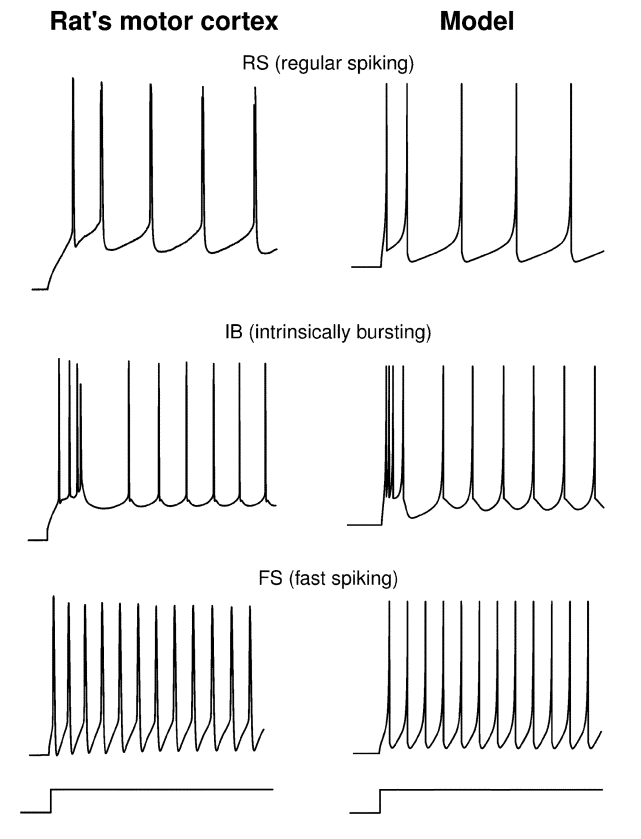
\includegraphics[width=0.5\linewidth]{images/patrones_disparo_izhikevich.png}
    \caption{Patrones de disparo del modelo neuronal Izhikevich. Extraído de Izhikevich \cite{Izhikevich2003}.}
    \label{fig:patrones_disparo_izhikevich}
\end{figure}

En el modelo, $v$ representa el potencial de membrana efectivo de la neurona y se escala en unidades comparables a milivoltios, con un potencial de reposo típico entre aproximadamente $-70$ y $-60 mV$ según el parámetro de acoplamiento \cite{Izhikevich2003}. La variable $u$ es una variable de recuperación que integra el efecto combinado de la activación de corrientes de potasio y de la inactivación de corrientes de sodio, proporcionando una realimentación negativa lenta sobre $v$. Esta variable $u$ permite capturar fenómenos como la adaptación de frecuencia, los pospotenciales hiperpolarizantes y ciertas oscilaciones subumbrales en un espacio de estados bidimensional, lo cual simplifica el análisis dinámico respecto de modelos de mayor dimensión.

El parámetro $a$ controla la escala temporal de la variable de recuperación $u$, de modo que valores pequeños de $a$ producen recuperaciones lentas y valores grandes generan dinámicas de recuperación más rápidas. El parámetro $b$ regula la sensibilidad de 
$u$ a las variaciones subumbrales del potencial de membrana $v$, y acoplamientos más fuertes pueden inducir oscilaciones subumbrales o disparo de umbral bajo. El parámetro $c$ fija el valor de reinicio del potencial de membrana después del disparo, representando el efecto de conductancias de potasio de alto umbral que llevan el potencial a niveles hiperpolarizados; un valor típico es $c\approx-65mV$ para neuronas de disparo regular. El parámetro $d$ determina el incremento de la variable de recuperación $u$ tras cada potencial de acción, lo que modela la acumulación de corrientes lentas y controla el grado de adaptación de frecuencia u otros regímenes dinámicos. Combinaciones específicas de $(a,b,c,d)$ permiten mapear distintos tipos de neuronas, lo que convierte a este modelo en un esquema parametrizable para múltiples fenotipos de disparo.

Mediante una elección adecuada de $(a,b,c,d)$, el modelo reproduce el disparo regular (\textit{regular spiking}, RS) característico de muchas neuronas piramidales. El modelo es capaz de producir muchos patrones de disparo que pueden ser usados en diferentes situaciones. Los diferentes modelos y comportamientos neuronales se pueden observar en las Figuras \ref{fig:patrones_disparo_izhikevich} y \ref{fig:disparos_izhikevich}.

\begin{figure}
    \centering
    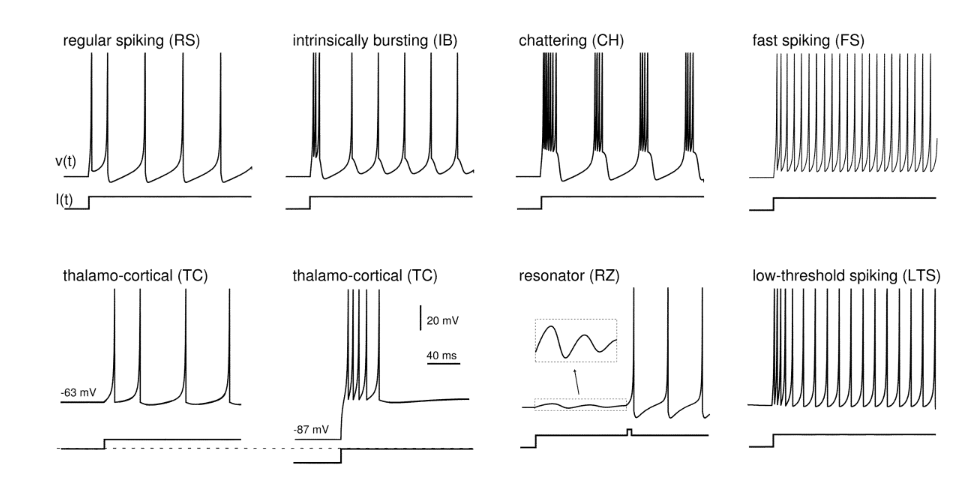
\includegraphics[width=1\linewidth]{images/disparos_izhikevich.png}
    \caption{Tipos de neuronas correspondiente a diferentes valores de a, b, c y d. Extraído de Izhikevich \cite{Izhikevich2003}.}
    \label{fig:disparos_izhikevich}
\end{figure}

La presente tesis adopta el modelo de Izhikevich porque ofrece un compromiso explícito entre plausibilidad biológica y eficiencia computacional, permitiendo simular redes de decenas de miles de neuronas en tiempo real con resolución del orden de milisegundos en hardware convencional. Esta eficiencia resulta especialmente adecuada para el escenario de optimización evolutiva multiobjetivo y esparsa a gran escala que se aborda en este trabajo, donde es necesario evaluar iterativamente un gran número de configuraciones de redes de disparo. Al mantener solo dos variables de estado continuas y una no linealidad cuadrática, el modelo facilita el estudio sistemático de patrones de disparo y regímenes de operación de SNN. Adicionalmente, el hecho de que el modelo sea canónico en el sentido de que puede derivarse de modelos de conductancias tipo Hodgkin–Huxley mediante reducciones apropiadas respalda su uso como representación compacta de neuronas biológicamente realistas en contextos de computación neuromórfica.

%--------------------------------

\section{Codificación y decodificación de spikes}\label{sec:codificacion-y-deco}

En una red neuronal de espigas, el codificador es el mecanismo que convierte datos continuos o discretos en trenes de espigas adecuados para su procesamiento temporal \cite{Wang2019spiketrainkernels, MAASS19971659ssnthirdgeneration}, mientras que el decodificador transforma estos trenes de espigas de salida en decisiones o valores numéricos interpretables \cite{Tavanaei2019dlinsnn, Schuman2022Opportunities}. Estos mecanismos son necesarios porque las SNN operan sobre eventos binarios en el tiempo \cite{Schuman2022Opportunities}, pudiendo aplicarse en la capa de entrada para transformar características como píxeles o variables sensoriales en espigas, mientras que la decodificación se emplea en la capa de salida para leer la clase o el valor estimado a partir de la actividad final \cite{Wang2019spiketrainkernels}.

\paragraph{Codificación Poisson (rate coding)} En el \textit{rate coding}, cada característica de entrada se representa mediante un tren de espigas cuya frecuencia media de disparo es proporcional al valor de la señal, de modo que entradas más grandes producen tasas de disparo más altas en una ventana temporal fija \cite{Guo2021neuronalcodingsnn}. Un modelo habitual para este tipo de codificación es el proceso de Poisson, en el que el número de espigas generadas en un intervalo de tiempo sigue una distribución de Poisson con parámetro $\lambda t$ que depende de la magnitud de la entrada \cite{Pachitariu2002modelsspiketrains, Yamazaki2022snnapplications}. En implementaciones prácticas de SNN, esta codificación Poisson suele aproximarse generando en cada paso de simulación una espiga con probabilidad proporcional al valor normalizado de la característica, lo que conduce a un tren de spikes estocástico cuya tasa de disparo coincide, en promedio, con la intensidad deseada \cite{Pachitariu2002modelsspiketrains}. Para decodificar bajo rate coding en tareas de clasificación, es común acumular el número de espigas de cada neurona de salida en una ventana de tiempo y seleccionar como clase predicha aquella neurona con mayor conteo de spikes \cite{Guo2021neuronalcodingsnn}.

\paragraph{Time‑to‑first‑spike (TTFS)}
En la codificación time‑to‑first‑spike (TTFS), la información se representa mediante la latencia del primer disparo: cada neurona de entrada emite a lo sumo una espiga y el tiempo hasta esa primera espiga codifica la intensidad del estímulo, de modo que valores más altos suelen corresponder a spikes más tempranos \cite{Guo2021neuronalcodingsnn, Bonilla2022ttfs}. Diversos trabajos teóricos y experimentales han mostrado que un código de latencia puede transmitir gran cantidad de información con muy pocas espigas, lo que permite decisiones muy rápidas y potencialmente un consumo energético reducido en hardware neuromórfico \cite{Bonilla2022ttfs}. En particular, estudios comparativos de esquemas de codificación en SNN profundas convertidas desde redes artificiales han demostrado que TTFS puede mayor exactitud de clasificación, con la menor latencia de inferencia y el número más bajo de operaciones sinápticas frente a rate coding y otros códigos temporales \cite{Guo2021neuronalcodingsnn}. La decodificación en redes TTFS suele basarse en reglas de “primero en disparar”, en las que la clase se asigna a la neurona de salida cuya espiga aparece con menor latencia dentro de una ventana de observación \cite{Bonilla2022ttfs, Goltz2021ttfsdeeplearning}.

\paragraph{Winner‑takes‑all (WTA)}
Winner‑takes‑all (WTA) es un principio de cómputo competitivo en el que un conjunto de neuronas recibe entradas similares y, a través de interacción selectiva, solo una neurona o un pequeño subconjunto queda finalmente activa, típicamente la que recibe el estímulo más fuerte \cite{Oster2009wtaspikes}. En redes de espigas, estos mecanismos WTA se han utilizado como bloques de decisión para categorización, selección de acciones y modelos atencionales, dado que permiten transformar un patrón complejo de actividad de población en una salida discreta fácilmente interpretable. En el contexto de decodificación en SNN, una regla WTA puede aplicarse tanto sobre el conteo de espigas en ventanas temporales (gana la neurona con mayor tasa) como sobre la latencia del primer disparo (gana la neurona que dispara antes), proporcionando una decisión “one‑hot” a partir del patrón temporal de la población de salida \cite{Guo2021neuronalcodingsnn}. Este tipo de decodificación permite asociar directamente cada neurona de salida a una clase concreta, lo que simplifica la lectura de resultados y el diseño de arquitecturas de clasificación supervisada basadas en SNN \cite{Schuman2022Opportunities}.

%---------------------------

%--------------------------------


\section{Optimización multiobjetivo}\label{sec:optimizacion-multi}
% \subsection{Definición y características}
La optimización multiobjetivo se ocupa de la minimización o maximización simultánea de un vector de funciones objetivo $f(x)=(f_1(x),...,f_m(x))$ sujeto a restricciones sobre las variables de decisión y el espacio factible. En estos problemas, los objetivos suelen ser conflictivos, de modo que no existe en general una sola combinación de variables que optimice todos los objetivos a la vez, sino un conjunto de soluciones que representan los mejores compromisos posibles \cite{Narayan2019optimization}. Así, la tarea del algoritmo no es encontrar un único óptimo global, sino generar y seleccionar puntos de solución no inferiores (no dominados) que materializan diferentes equilibrios entre los objetivos en competencia \cite{Narayan2019optimization}.

Formalmente, un problema de optimización multiobjetivo puede expresarse como encontrar $x\in \Omega$ que minimice el vector $f(x)=(f_1(x),...,f_m(x))$, donde $\Omega$ denota el conjunto de soluciones factibles definido por restricciones de igualdad, desigualdad y cotas \cite{MathWorksMultiobjectiveOptimization}. Cada componente cuantifica un criterio de desempeño distinto (por ejemplo, error de clasificación, complejidad del modelo o consumo de recursos), y la naturaleza multiobjetivo surge cuando estos criterios no pueden mejorarse simultáneamente sin degradar al menos uno de ellos \cite{Narayan2019optimization}. En este contexto, el concepto de optimalidad se redefine en términos de dominancia de Pareto, y las soluciones relevantes son aquellas que no son superadas simultáneamente en todos los objetivos por ninguna otra solución factible \cite{Narayan2019optimization}.

La dominancia de Pareto define una relación de orden sobre el conjunto de soluciones, basada en la comparación componente a componente de sus vectores de objetivo \cite{Deb2011MOEAintro}. Asumiendo problemas de minimización, se dice que una solución \(x\) domina a otra solución \(y\), lo que se denota como \(x \succ y\), si \(x\) no es peor que \(y\) en todos los objetivos y es estrictamente mejor en al menos uno de ellos \cite{Deb2011MOEAintro}. Por consiguiente, una solución se considera Pareto óptima si no es dominada por ninguna otra solución factible \cite{Deb2011MOEAintro}.

El conjunto de todas las soluciones Pareto óptimas en el espacio de decisión se denomina conjunto de Pareto, mientras que su imagen en el espacio de objetivos se conoce como frente de Pareto \cite{Deb2011MOEAintro}. En consecuencia, el frente de Pareto está compuesto por vectores objetivo no dominados, los cuales representan compromisos óptimos: mejorar un objetivo implica necesariamente deteriorar al menos otro. Desde la perspectiva de la toma de decisiones, este frente proporciona un conjunto de alternativas entre las que un decisor puede seleccionar una solución de acuerdo con sus preferencias o restricciones adicionales \cite{MathWorksMultiobjectiveOptimization, Narayan2019optimization}.

Al diseñar algoritmos de optimización multiobjetivo, se persiguen dos metas fundamentales: lograr una buena convergencia hacia el frente de Pareto verdadero y mantener una adecuada diversidad a lo largo de dicho frente \cite{Panichella2022paretofront}. La convergencia se refiere a la proximidad del conjunto aproximado de soluciones al frente de Pareto real, medida típicamente mediante distancias en el espacio de objetivos o indicadores de error de aproximación \cite{Panichella2022paretofront,Gong2020evolutionaryoptimization}. La diversidad, por su parte, alude a cuán bien distribuidas están las soluciones sobre el frente, buscando una cobertura uniforme de las distintas regiones de compromiso para facilitar una toma de decisiones informada \cite{Panichella2022paretofront}. En la práctica, muchos algoritmos evolucionarios multiobjetivo utilizan la dominancia de Pareto para guiar la convergencia y operadores de densidad o dispersión (por ejemplo, distancia de crowding) para preservar la diversidad dentro de la población \cite{Gong2020evolutionaryoptimization, Panichella2022paretofront}.

En el contexto de redes neuronales (incluyendo redes de espigas), existe un compromiso bien documentado entre exactitud de clasificación y eficiencia computacional, donde esta última puede modelarse mediante medidas de esparsidad estructural o de pesos \cite{Suidgeest2024snnthesis, khan2026hierarchicalimportanceguidedmultiobjectiveevolutionary}. La esparsidad cuantifica la proporción de parámetros o sinapsis inactivos dentro de una red. Por tanto, una mayor esparsidad implica un menor número de conexiones activas, lo que puede reducir los requerimientos de cómputo y memoria cuando la arquitectura o el hardware logran explotar dicha estructura. Sin embargo, niveles excesivos de esparsidad pueden afectar negativamente la exactitud del modelo al eliminar conexiones relevantes para la tarea \cite{dimovska2020multiobjectiveoptimizationsizeresilience, Suidgeest2024snnthesis}. Diversos trabajos formulan el diseño y la poda de redes neuronales como un problema de optimización multiobjetivo en el que se minimiza simultáneamente el error de clasificación y una medida de complejidad del modelo basada en el número de pesos no nulos o neuronas activas \cite{Yue2025CNEA, MOEA/CKF, khan2026hierarchicalimportanceguidedmultiobjectiveevolutionary, dimovska2020multiobjectiveoptimizationsizeresilience}. En SNN, se ha mostrado que minimizar de manera explícita la complejidad estructural de la red, junto con la  minimización del error, permite obtener arquitecturas más compactas que preservan el rendimiento predictivo dentro de márgenes aceptables \cite{khan2026hierarchicalimportanceguidedmultiobjectiveevolutionary, dimovska2020multiobjectiveoptimizationsizeresilience}. Formular el problema con estos dos objetivos explícitos proporciona al algoritmo multiobjetivo un criterio claro para explorar el compromiso exactitud–esparsidad, generando un frente de Pareto que expone soluciones desde modelos densos y muy precisos hasta modelos altamente esparsos y más eficientes, entre los cuales el investigador puede seleccionar según los requisitos de la aplicación \cite{Suidgeest2024snnthesis, dimovska2020multiobjectiveoptimizationsizeresilience}.


% \subsection{Métricas de calidad y evaluación del frente}
En optimización multiobjetivo, la calidad de un conjunto aproximado del frente de Pareto se evalúa típicamente a partir de dos aspectos principales: la convergencia hacia el frente verdadero y la diversidad o distribución de las soluciones a lo largo de dicho frente \cite{RAVBER2017qualityindicatorsMOEA}. Para comparar rigurosamente diferentes algoritmos, la literatura recomienda emplear indicadores cuantitativos que midan simultáneamente cuán cerca está el frente aproximado del frente óptimo y qué tan bien cubre la región de compromisos de interés \cite{Shao2025_SMOEA}.

Entre los indicadores de calidad más utilizados se encuentra el Hipervolumen (HV), que mide el volumen de la región del espacio objetivo que queda dominada por el conjunto aproximado con respecto a un punto de referencia dado \cite{Auger2009HV, AUGER2012hv}. Este indicador es especialmente atractivo porque es estrictamente compatible con la dominancia de Pareto, es decir, si un conjunto de soluciones domina completamente a otro, entonces su hipervolumen es necesariamente mayor \cite{Zitzler2007HV_revisited, Auger2009HV}. Además, al integrar simultáneamente información de convergencia (al maximizar la región dominada cercana al frente verdadero) y de diversidad (al premiar conjuntos que cubren una mayor extensión del frente), el HV se considera un indicador global de la calidad del frente aproximado \cite{Jiang2015HVMEOA, Auger2009HV}.

En el contexto del entrenamiento de redes neuronales (incluidas las SNN), suele combinarse al menos una métrica de desempeño en la tarea, como la exactitud o el error de clasificación, con indicadores multiobjetivo como HV o IGD para evaluar la calidad del frente de Pareto obtenido por el algoritmo evolutivo \cite{Zitzler2007HV_revisited, RAVBER2017qualityindicatorsMOEA, Santos2018convergenceindicator}. De este modo, la evaluación no se limita a comparar un único modelo, sino que analiza el conjunto de soluciones que representan diferentes compromisos entre exactitud y complejidad estructural (por ejemplo, esparsidad de la red), permitiendo caracterizar de forma más completa la capacidad del algoritmo para aproximar frentes de Pareto relevantes para la aplicación \cite{RAVBER2017qualityindicatorsMOEA, Zitzler2007HV_revisited}.
	\chapter{Estado del arte}

\section{Aprendizaje en SNN}

El aprendizaje en SNN se enfrenta a desafíos específicos derivados de la naturaleza binaria y asincrónica de los spikes, así como de la dinámica temporal explícita de las neuronas y sinapsis. \cite{Neftci2019SurrogateGradient, Zenke2021surrogatesnn}. En la literatura se han desarrollado principalmente cinco familias de enfoques: entrenamiento directo mediante gradientes (p. ej. gradientes sustitutos), conversión ANN–SNN, reglas de plasticidad sináptica tipo plasticidad dependiente del tiempo de disparo (Spike-Timing-Dependent Plasticity, STDP), computación de reservorio y métodos de Neuroevolución que optimizan pesos y arquitectura \cite{Bittar2022surrogatespiking, Moisy2006snnsurvey}.

\subsection{Limitaciones del Backpropagation clásico en SNN}
El algoritmo del \textit{Backpropagation} clásico, desarrollado para neuronas con activaciones continuas y derivables, no es directamente aplicable a SNN porque la función de disparo es típicamente una no linealidad tipo función escalón de Heaviside, no derivable y con gradiente nulo casi en todas partes \cite{Zenke2021surrogatesnn}. Adicionalmente, el aprendizaje supervisado en SNN requiere tratar la dimensión temporal de forma explícita, lo que lleva a variantes de Backpropagation Through Time (BPTT) con costes computacionales elevados y problemas de desvanecimiento de gradientes o explosivos sobre horizontes de simulación largos \cite{Neftci2019SurrogateGradient, Bittar2022surrogatespiking}.

En SNN biológicamente plausibles, la dinámica de membrana y de sinapsis introduce estados internos de memoria que complican aún más la asignación de crédito temporal, pues los efectos de un spike presináptico pueden manifestarse tras múltiples pasos de tiempo \cite{Moisy2006snnsurvey}. Por otra parte, la implementación eficiente en hardware neuromórfico exige mantener una actividad de disparo muy dispersa (sparse), lo que agrava los problemas de estimación de gradientes \cite{Li2024snnsparsesurrogate, Schuman2022Opportunities}.

Estas limitaciones han motivado la aparición de métodos alternativos de entrenamiento que aproximan o evitan el cálculo exacto del gradiente, tales como los gradientes sustitutos, la conversión ANN–SNN y los enfoques basados en plasticidad sináptica o en algoritmos evolutivos \cite{Shen2024EvolutionarySNN, Schuman2022Opportunities}.

\subsection{Alternativas al uso de Backpropagation}
A pesar de las limitaciones del Backpropagation en SNN, existen alternativas al entrenamiento de SNN usando algunos métodos y técnicas que se describen a continuación.

\paragraph{Gradientes sustitutos (surrogate gradients)}
Los métodos de gradientes sustitutos aproximan la derivada de la función de disparo no diferenciable mediante una función suave (por ejemplo sigmoide, triangular o cuadrática), lo que permite aplicar variantes de descenso por gradiente y BPTT en SNN de forma análoga a las redes artificiales clásicas \cite{Zenke2021surrogatesnn}. En estos enfoques, durante la fase hacia adelante se mantiene la dinámica de disparo binaria, mientras que en la fase hacia atrás se reemplaza la derivada nula por una aproximación diferenciable en un vecindario del umbral, lo que hace posible propagar señales de error útiles \cite{Neftci2019SurrogateGradient}.

Diversos estudios han mostrado que el aprendizaje con gradientes sustitutos puede alcanzar desempeños competitivos con ANN en tareas de clasificación y reconocimiento de patrones, manteniendo al mismo tiempo ciertas ventajas de eficiencia energética al ejecutarse sobre hardware neuromórfico \cite{Zenke2021surrogatesnn, Schuman2022Opportunities}. Los resultados muestran que el entrenamiento con gradientes sustitutos no depende demasiado de la forma exacta de la función usada como aproximación de la derivada. Sin embargo, sí es importante ajustar adecuadamente su escala y añadir una penalización sobre la actividad de disparo, para evitar redes con demasiados spikes y conservar la esparsidad deseada \cite{Li2024snnsparsesurrogate}.

Trabajos recientes han propuesto extensiones como gradientes sustitutos enmascarados (Masked Surrogate Gradients), que buscan equilibrar la eficacia del entrenamiento con la dispersidad del gradiente, mejorando la capacidad de generalización de las SNN \cite{Li2024snnsparsesurrogate}. Asimismo, se han reportado aplicaciones exitosas de gradientes sustitutos en dominios de procesamiento de voz y comandos de habla, donde SNN entrenadas directamente con este enfoque alcanzan precisiones comparables a arquitecturas ANN convencionales \cite{Bittar2022surrogatespiking}.

\paragraph{Conversión ANN-SNN}
Una alternativa al entrenamiento directo consiste en entrenar primero una red neuronal artificial (ANN) con activaciones continuas (por ejemplo ReLU) y posteriormente convertirla en una SNN manteniendo su topología, trasladando los pesos y ajustando umbrales y codificación temporal \cite{Jiang2023anntosnn, Schuman2022Opportunities}. Esta clase de métodos ha demostrado que es posible obtener SNN profundas con precisiones cercanas a las ANN de origen en conjuntos de datos de gran escala como CIFAR \cite{cifar-10} o ImageNet, aunque el compromiso entre latencia (número de pasos de tiempo) y exactitud sigue siendo un problema central \cite{Ding2021anntosnnoptimal, Gao2023anntosnnbipolarlif}. Para reducir el error de conversión y la latencia, se han propuesto modificaciones en las activaciones de la ANN de origen, como capas específicas de normalización de tasa o funciones ReLU modificadas y cuantizadas que aproximan mejor el comportamiento de neuronas de disparo \cite{Ding2021anntosnnoptimal}.

% También se ha explorado la integración con otras técnicas como entrenamiento consciente de cuantización (quantization-aware training) en el proceso de conversión, evitando fases de postprocesado costosas \cite{Gao2023anntosnnbipolarlif, Jiang2023anntosnn}. Más recientemente, se han introducido esquemas de codificación diferencial que transmiten cambios incrementales de tasa en lugar de tasas absolutas, lo que reduce el número de spikes y el consumo energético sin necesidad de entrenamiento adicional tras la conversión \cite{huang2025differentialanntosnn}.

\paragraph{Plasticidad sináptica (STDP y variantes)}
La plasticidad dependiente del tiempo de disparo (Spike-Timing Dependent Plasticity, STDP) es una regla de aprendizaje inspirada en observaciones neurobiológicas, donde el cambio de peso sináptico depende de la diferencia temporal entre los spikes pre y postsinápticos \cite{RAHMAN2025stdp}. En su forma clásica, los spikes presinápticos que preceden ligeramente a los spikes postsinápticos inducen potenciación de la sinapsis, mientras que spikes postsinápticos anteriores a los presinápticos conducen a depresión, implementando una versión temporizada de aprendizaje Hebbiano \cite{Moisy2006snnsurvey, RAHMAN2025stdp}.

STDP se ha utilizado ampliamente como regla de aprendizaje no supervisado en SNN, permitiendo que las redes aprendan características relevantes de los datos de entrada, y ha sido aplicada sobre hardware emergente como memorias resistivas (RRAM) para aprendizaje en línea \cite{Guo2019rramsnn}. No obstante, algunas variantes de STDP incorporan señales de refuerzo o neuromodulación, lo que permite extender el esquema a escenarios de aprendizaje por refuerzo y supervisado aproximado \cite{RAHMAN2025stdp}.

% Por ejemplo, se han propuesto reglas de STDP moduladas por recompensa (Reward-Modulated STDP, RM‑STDP) que combinan correlaciones temporales locales con señales de recompensa global, logrando resolver tareas no linealmente separables como XOR en configuraciones de computación de reservorio basadas en SNN.

% Además, se han introducido variantes como STDP basada en ensamblajes (assembly-based STDP), que organizan neuronas en conjuntos funcionales y fortalecen selectivamente las conexiones intra-ensamblaje mientras inhiben conexiones inter-ensamblaje para mejorar la capacidad de representación jerárquica.

Aunque STDP y sus extensiones ofrecen una alta plausibilidad biológica y se adaptan bien a implementaciones locales en hardware, presentan desafíos importantes de escalabilidad, sensibilidad a hiperparámetros y dificultad para imponer objetivos globales de tarea en redes profundas \cite{Saranirad2022stdp, RAHMAN2025stdp}.

\paragraph{Computación de reservorio}
El reservorio es una red recurrente de conexiones fijas y generadas aleatoriamente que, al recibir una entrada, actúa como un sistema dinámico no lineal capaz de proyectar la entrada a un espacio de estados de alta dimensión, sin necesidad de entrenamiento alguno \cite{LUKOSEVICIUS2009reservoir}. Teniendo eso en cuenta, la computación de reservorio es un paradigma en el que solo se entrenan los pesos de salida de una red recurrente, manteniendo fijos los pesos internos del reservorio, lo que simplifica el aprendizaje sobre dinámicas no lineales complejas \cite{LUKOSEVICIUS2009reservoir}. Los dos modelos pioneros son las Echo State Networks (ESN), basadas en neuronas de activación continua, y las Liquid State Machines (LSM), que emplean neuronas de espigas y sinapsis dinámicas, representando respectivamente la segunda y la tercera generación de redes neuronales \cite{LUKOSEVICIUS2009reservoir}.

En LSM, el reservorio consiste en una población de neuronas de espigas, donde los patrones de entrada pueden ser linealmente separados por una capa de lectura entrenable \cite{LUKOSEVICIUS2009reservoir}. Estas arquitecturas han demostrado ser capaces de resolver tareas que requieren memoria de corto plazo y no linealidad, como reconocimiento de habla, predicción de series temporales y detección de crisis epilépticas, si bien con un coste computacional mayor que ESN debido a la simulación de spikes \cite{Kholkin2023reservoirsnn}.

En el contexto de SNN, la computación de reservorio presenta la ventaja de evitar el entrenamiento de las conexiones recurrentes internas, delegando el aprendizaje a una capa de salida lineal o ligeramente no lineal que puede optimizarse mediante métodos clásicos de regresión o clasificación \cite{LUKOSEVICIUS2009reservoir}.

% CONSIDERAR PARAGRAPH
\paragraph{Neuroevolución}
La Neuroevolución emplea algoritmos evolutivos para optimizar redes neuronales, tratando pesos, topología y otros hiperparámetros como genotipos que se adaptan mediante operadores de selección, mutación y, en algunos casos, cruce \cite{Hiraga2024mutationbasedevolution}. A diferencia de los métodos basados en gradientes, la Neuroevolución no requiere usar la derivada en la función de coste, lo que la hace especialmente atractiva para problemas con funciones objetivo no diferenciables, ruidosas o definidas por simuladores complejos \cite{risi2025neuroevolution}. El flujo principal de los algoritmos evolutivos se puede ver en la Figura \ref{fig:ea-flujo}.

\begin{figure}
    \centering
    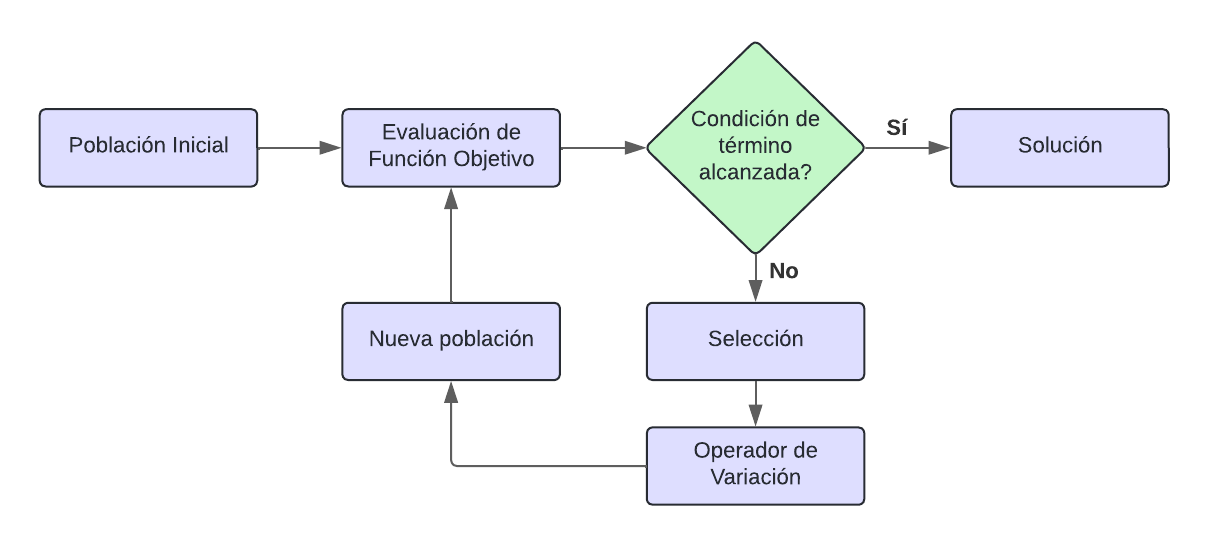
\includegraphics[width=0.8\linewidth]{images/ea-flujo.png}
    \caption{Flujo principal de un algoritmo evolutivo. Se comienza con un conjunto de soluciones candidatas que son evaluadas por una función objetivo. Basado en el desempeño, ciertas soluciones se eligen para producir variabilidad mediante operadores genéticos. El ciclo se repite hasta que se alcanza la condición de término. Adaptado de \cite{risi2025neuroevolution}.}
    \label{fig:ea-flujo}
\end{figure}

En redes neuronales artificiales profundas, se ha demostrado que algoritmos genéticos puros pueden escalar a redes con millones de parámetros, alcanzando rendimientos competitivos con métodos de aprendizaje profundo en tareas de control y refuerzo, lo que evidencia el potencial de la exploración poblacional a gran escala \cite{Stanley2019neuroevolution}. La Neuroevolución también permite optimizar simultáneamente la arquitectura (número de capas, conexiones, tipos de neuronas) y los pesos, abordando de manera unificada problemas de búsqueda de arquitectura neuronal que son difíciles de tratar con \textit{Backpropagation} \cite{Such2017deepneuroevolution, Schuman2022Opportunities}.

Las ventajas principales de la Neuroevolución incluyen: no depender de gradientes ni de funciones objetivo diferenciables, lo que permite optimizar también objetivos no diferenciables o ruidosos; optimizar simultáneamente pesos, arquitectura y otros hiperparámetros; y mantener diversidad poblacional, lo que favorece la exploración y la aparición de soluciones novedosas \cite{Hiraga2024mutationbasedevolution}. Estas características la hacen especialmente atractiva en escenarios donde la dinámica de la red o la función de aptitud se definen mediante simuladores complejos, con recompensas escasas o retardadas, o donde se desean incorporar explícitamente objetivos adicionales como robustez, interpretabilidad o eficiencia energética \cite{risi2025neuroevolution}.

En el ámbito de las SNN, han surgido enfoques evolutivos donde los algoritmos diseñan tanto la topología como los parámetros neuronales (por ejemplo constantes de tiempo y umbrales) y los esquemas de codificación de spikes, logrando redes energéticamente eficientes y de alto rendimiento en diferentes benchmarks \cite{Shen2024EvolutionarySNN}. Estudios recientes han mostrado que la elección del modelo neuronal (por ejemplo Izhikevich frente a LIF) y del esquema de codificación influye de manera crucial en el rendimiento de SNN evolucionadas, lo que resalta la importancia de configurar adecuadamente estos elementos durante la optimización evolutiva \cite{LoyolaJara2026evolvingsnn}.

Las principales ventajas de la Neuroevolución para SNN incluyen su naturaleza libre de gradientes, la capacidad de manejar funciones objetivo no diferenciables (como métricas de energía o esparsidad de spikes) y la posibilidad de optimizar explícitamente pesos, arquitecturas y parámetros neuronales bajo múltiples objetivos \cite{Shen2024EvolutionarySNN, Schuman2022Opportunities}. No obstante, estos métodos presentan desafíos significativos de coste computacional y escalabilidad, ya que requieren evaluar poblaciones completas de redes en cada generación y gestionar espacios de búsqueda de alta dimensión, lo que exige estrategias eficientes de muestreo, paralelización y reducción de complejidad \cite{Hiraga2024mutationbasedevolution, Such2017deepneuroevolution}.

En la literatura reciente se han propuesto marcos unificados que combinan Neuroevolución con aprendizaje por gradiente estocástico, así como algoritmos evolutivos capaces de trabajar con múltiples objetivos como precisión, complejidad del modelo y eficiencia energética, lo que resulta especialmente relevante para el diseño de SNN ejecutables en hardware neuromórfico bajo restricciones de recursos \cite{Zhang2023DNN_Neuroevolution_SGD, Shen2024EvolutionarySNN}. En este contexto, los métodos de optimización evolutiva multiobjetivo aplicados a SNN se alinean de forma natural con la necesidad de equilibrar desempeño, esparsidad y costo computacional en redes de disparo de gran escala, motivando la exploración de algoritmos avanzados de optimización poblacional y estrategias de codificación adecuadas para este tipo de modelos \cite{Shen2024EvolutionarySNN, Hiraga2024mutationbasedevolution}.


%---------------------

\section{Neuroevolución en SNN}
La Neuroevolución se refiere al uso de algoritmos evolutivos para diseñar y entrenar redes neuronales, tratando pesos, arquitectura y otros hiperparámetros como individuos de una población que se adapta mediante selección, mutación y recombinación \cite{Schuman2020evooptineuro, Shen2024EvolutionarySNN}. En el contexto de SNN, esta familia de métodos se ha consolidado como una alternativa a los enfoques basados en gradientes, especialmente cuando se busca optimizar simultáneamente la estructura de la red, los parámetros neuronales y criterios adicionales como eficiencia energética o tamaño del modelo \cite{Shen2024EvolutionarySNN, Schuman2022Opportunities}.

\subsection{Optimización en SNN}
Los trabajos de Neuroevolución aplicados a SNN se diferencian principalmente por el conjunto de elementos que deciden optimizar: pesos sinápticos, topología de la red, parámetros neuronales y esquemas de codificación y decodificación, así como métricas multiobjetivo asociadas al desempeño y la eficiencia estructural \cite{Schliebs2013snn-survey, Jin2007evo-multi-snn}. Los primeros enfoques se centraron en redes relativamente poco profundas, donde algoritmos como GA, PSO, DE y estrategias de armonía se utilizaron para ajustar pesos, retardos sinápticos y conectividad, abordando tareas de clasificación y control con arquitecturas de tamaño moderado \cite{Shen2024EvolutionarySNN}.

En el marco de EONS (Evolutionary Optimization for Neuromorphic Systems) \cite{Schuman2020evooptineuro}, Schuman y colaboradores proponen un esquema evolutivo que optimiza SNN representadas como grafos de nodos y aristas, donde cada nodo y cada sinapsis pueden asociar múltiples parámetros (por ejemplo, umbrales, fugas, pesos y retardos) que se ajustan evolutivamente, permitiendo determinar simultáneamente la estructura de la SNN y los parámetros específicos de cada elemento \cite{Schuman2020evooptineuro}, y se ha aplicado tanto a tareas de clasificación como de control, a problemas de diseño de reservorios y a optimización multiobjetivo orientada a minimizar el tamaño de la red \cite{Schuman2022Opportunities}.

Otros trabajos utilizan Neuroevolución principalmente para búsqueda de arquitecturas para posterior entrenamiento usando Backpropagation, integrando mecanismos como Neural Architecture Search (NAS) en el dominio de las SNN; por ejemplo, los enfoques AutoSNN, SpikeDHS, NeuEvo y STTS emplean algoritmos evolutivos o híbridos para escoger bloques de convolución, tamaños de kernel, conexiones recurrentes y tipos de operadores de disparo, con énfasis en el compromiso entre precisión, tasa de espigas y coste computacional \cite{Shen2024EvolutionarySNN}, y se han reportado arquitecturas que alcanzan precisiones competitivas en CIFAR, ImageNet y tareas sobre datos de eventos, manteniendo un número de operaciones sinápticas significativamente menor que redes artificiales equivalentes \cite{Shen2024EvolutionarySNN}.

También existe una línea de trabajo centrada en la optimización directa de la arquitectura y los hiperparámetros de SNN mediante marcos de Neuroevolución generalistas, como SPENSER \cite{Branquinho2023-neuro-conv-snn}, que extiende un framework evolutivo originalmente diseñado para ANN (DENSER) al caso de SNN convolucionales, generando redes con rendimiento competitivo en tareas de clasificación estática.

Finalmente, una línea particularmente relevante para esta tesis considera la optimización multiobjetivo de SNN, donde algoritmos evolutivos buscan simultáneamente minimizar el error de clasificación y reducir el tamaño o la complejidad de la red, dando lugar a frentes de Pareto que exponen el compromiso entre exactitud y esparsidad \cite{Schuman2022Opportunities, Jin2007evo-multi-snn}. En estos trabajos, los objetivos incluyen típicamente métricas de desempeño (exactitud, error) y medidas estructurales como número de neuronas activas, porcentaje de conexiones no nulas o estimaciones de consumo energético asociadas al número de operaciones sinápticas, lo que se alinea de forma directa con el enfoque de optimización esparsa considerado en este trabajo de título \cite{dimovska2020multiobjectiveoptimizationsizeresilience}.


\subsection{Ventajas del enfoque evolutivo en SNN}
Una de las ventajas más citadas de la Neuroevolución en el contexto de SNN es que los algoritmos evolutivos no requieren información de gradiente, por lo que pueden trabajar directamente con funciones de activación no diferenciables, dinámicas temporales complejas y simuladores neuromórficos que no ofrecen derivadas de la función de coste \cite{Schuman2022Opportunities, Schuman2020evooptineuro}. Esta independencia de gradientes permite aplicar los métodos evolutivos a arquitecturas recurrentes, redes con retardos axonales y sinápticos, y modelos neuronales biológicamente plausibles (como Izhikevich \cite{Izhikevich2003} o LIF \cite{Gao2023anntosnnbipolarlif}) sin modificar sus ecuaciones subyacentes, lo que constituye una ventaja frente a los enfoques basados en gradientes sustitutos \cite{Shen2024EvolutionarySNN}.

Otra ventaja relevante es la capacidad de optimizar simultáneamente la estructura y los parámetros de la red, abarcando desde el número de neuronas y capas hasta el patrón de conectividad y los valores de umbral, pesos y retardos, tal como se ejemplifica en EONS y en marcos inspirados en NEAT \cite{Schuman2020evooptineuro, Stanley2002NEAT}. Este tratamiento unificado del diseño de arquitectura y del ajuste de parámetros permite explorar configuraciones que serían difíciles de alcanzar mediante procedimientos clásicos haciendo uso de gradientes, y facilita la aparición de topologías no convencionales que utilizan ciclos, conexiones cruzadas e interacciones complejas entre capas \cite{Elbrecht2020-neuro-snn, Schuman2020evooptineuro}.

Los algoritmos evolutivos también se adaptan de forma natural a escenarios multiobjetivo, incorporando explícitamente objetivos como exactitud, tamaño de la red, consumo energético o robustez frente a perturbaciones, y utilizando indicadores como Hipervolumen o IGD para evaluar la calidad del conjunto de soluciones encontradas \cite{Jin2007evo-multi-snn, dimovska2020multiobjectiveoptimizationsizeresilience}. En el contexto neuromórfico, esta capacidad resulta especialmente útil cuando se desea reducir el número de conexiones activas, limitar el rango de pesos o respetar restricciones de resolución y retardos impuestos por el hardware, sin perder de vista el rendimiento en la tarea de clasificación o control \cite{Branquinho2023-neuro-conv-snn, Schuman2020evooptineuro, Schuman2022Opportunities}.

Otro aspecto ventajoso es la compatibilidad de los métodos evolutivos con tareas de control y refuerzo, donde la función objetivo puede ser no diferenciable, ruidosa o definida por simuladores complejos; diversos trabajos han mostrado que estrategias evolutivas pueden entrenar SNN para problemas como navegación de robots y juegos, alcanzando comportamientos comparables o superiores a reglas de plasticidad locales como STDP-RL \cite{Hasegan2022snn-rl, Shen2024EvolutionarySNN}.

Finalmente, los enfoques evolutivos ofrecen una integración relativamente directa con plataformas neuromórficas reales, ya que pueden incluir en la representación genética los límites de hardware (por ejemplo, resolución de pesos, número máximo de retardos, topologías permitidas) y evolucionar únicamente redes que sean realizables bajo dichas restricciones.

%--------

\subsection{Limitaciones actuales y desafíos}
A pesar de sus ventajas, los métodos evolutivos aplicados a SNN presentan limitaciones importantes en términos de coste computacional, ya que requieren evaluar poblaciones completas de redes en cada generación, y cada evaluación implica simulaciones temporales potencialmente largas sobre conjuntos de datos de entrenamiento \cite{Schuman2022Opportunities, Schuman2020evooptineuro}. Esta naturaleza poblacional hace que la Neuroevolución sea, en muchos casos, más lenta para converger que los enfoques basados en gradientes, especialmente cuando se trabaja con redes profundas y datasets de gran escala, lo que ha motivado el desarrollo de estrategias de reducción de coste y búsqueda más eficiente \cite{Shen2024EvolutionarySNN, Branquinho2023-neuro-conv-snn}.

Históricamente, muchas aplicaciones evolutivas en SNN se han limitado a arquitecturas relativamente poco profundas o a problemas con pocas entradas, debido tanto a restricciones de hardware como a la complejidad de simular grandes SNN; aunque trabajos recientes han extendido estos métodos a SNN profundas y convolucionales, todavía existe una brecha respecto del rendimiento y la escala alcanzados por redes artificiales entrenadas con gradientes sustitutos o conversión ANN-SNN \cite{Branquinho2023-neuro-conv-snn, Schliebs2013snn-survey}. Algunos estudios \cite{Shen2024EvolutionarySNN} señalan que aunque enfoques como SpikeDHS, STTS, AutoSNN y NeuEvo logran precisiones competitivas en CIFAR e ImageNet, muchos de ellos dependen de espacios de búsqueda complejos, entrenamiento de superredes o combinaciones con técnicas basadas en gradientes, lo que evidencia que la Neuroevolución pura aún enfrenta desafíos en tareas de muy gran escala.

Otro desafío importante reside en el diseño del espacio de búsqueda y la codificación genética de las redes, ya que la elección de cómo representar arquitectura, pesos, retardos y operadores de disparo influye de manera crítica en la capacidad del algoritmo evolutivo para explorar soluciones útiles sin perder eficiencia \cite{Elbrecht2020-neuro-snn}. Además, existe aún poca homogeneidad en la literatura respecto de los criterios de evaluación y los benchmarks utilizados para comparar métodos evolutivos en SNN, lo que dificulta construir una imagen clara de cuál enfoque ofrece el mejor compromiso entre precisión, esparsidad y coste computacional \cite{Shen2024EvolutionarySNN}. Algunos trabajos reportan únicamente métricas de exactitud, mientras que otros añaden medidas de tasa de espigas, número de sinapsis activas o estimaciones de consumo energético. La falta de conjuntos de pruebas estandarizados para SNN evolutivas hace que los resultados sean, en muchos casos, difíciles de trasladar entre dominios y plataformas de hardware \cite{dimovska2020multiobjectiveoptimizationsizeresilience, Shen2024EvolutionarySNN}.

Finalmente, aunque las aproximaciones evolutivas han mostrado resultados prometedores en aplicaciones de control y clasificación, su combinación con requisitos estrictos de esparsidad y gran escala sigue siendo un problema abierto, donde la búsqueda de arquitecturas extremadamente ligeras y redes altamente eficientes debe equilibrarse con la necesidad de mantener un rendimiento comparable al de enfoques basados en gradientes \cite{dimovska2020multiobjectiveoptimizationsizeresilience, Schuman2020evooptineuro}. Esta tensión entre exploración evolutiva, exigencias de hardware neuromórfico y objetivos multiobjetivo complejos motiva el desarrollo de algoritmos evolutivos especializados para problemas esparsos de gran escala, como los SMOEA considerados en esta tesis, que buscan mejorar la capacidad de las SNN evolutivas para operar en escenarios donde la eficiencia estructural es tan relevante como la precisión \cite{Shen2024EvolutionarySNN, Schuman2022Opportunities}.

%------------

\section{Esparsidad y eficiencia estructural de redes neuronales}

\subsection{Definición}
En el contexto de redes neuronales profundas y SNN, se entiende por modelo esparso aquel en que una fracción significativa de los parámetros o conexiones toma el valor cero, de modo que solo un subconjunto reducido de sinapsis participa efectivamente en el cómputo \cite{REINERS2022sparse, Huang2021sparse-opti-multi}. Esta reducción explícita de conexiones activas se traduce en una menor complejidad estructural del modelo, con impacto directo sobre el número de operaciones requeridas, el uso de memoria y, en plataformas neuromórficas, el consumo energético asociado a eventos sinápticos \cite{LIAN2024-multi-cnn-ea, Schuman2022Opportunities, REINERS2022sparse}.

Diversos trabajos sobre poda y compresión de redes neuronales formulan la búsqueda de arquitecturas esparsas como un problema de optimización multiobjetivo, donde se busca simultáneamente preservar el desempeño predictivo y disminuir la complejidad estructural del modelo \cite{Huang2021sparse-opti-multi, REINERS2022sparse}. En el caso particular de SNN, estudios recientes \cite{dimovska2020multiobjectiveoptimizationsizeresilience, Schuman2022Opportunities} han mostrado que minimizar de forma explícita el tamaño o número de conexiones de la red puede incrementar la resiliencia a fallos hardware y reducir el coste de implementación en arquitecturas neuromórficas, manteniendo una precisión de clasificación aceptable.

Así, la esparsidad pasa a constituir un objetivo explícito de diseño, que debe equilibrarse con la exactitud y otras métricas de rendimiento mediante por ejemplo, técnicas de optimización basada en poblaciones como los algoritmos evolutivos \cite{REINERS2022sparse, Huang2021sparse-opti-multi}. Este enfoque resulta coherente con la motivación neuromórfica de la tesis, donde el entrenamiento de SNN busca no solo resolver correctamente tareas de clasificación, sino hacerlo con redes estructuralmente ligeras y eficientes en términos de recursos computacionales \cite{dimovska2020multiobjectiveoptimizationsizeresilience, Schuman2022Opportunities}.

En la literatura de poda de redes densas se distingue entre esparsidad no estructurada y esparsidad estructurada \cite{Yang2019-mo-cnn-ga, LIAN2024-multi-cnn-ea}. Los métodos de poda no estructurada generan patrones irregulares de pesos nulos que pueden ser difíciles de explotar en hardware convencional, ya que las bibliotecas estándar de convolución no suelen estar optimizadas para kernels extremadamente dispersos sin soporte especializado \cite{HIRSCH2022-mo-dnn-drl, LIAN2024-multi-cnn-ea}. 

En cambio, la esparsidad estructurada tiende a traducirse en reducciones más evidentes del coste computacional, ya que elimina operaciones completas asociadas a filtros o canales y permite reutilizar implementaciones de convolución estándar con menores dimensiones efectivas \cite{Chen2021-sparse-nn-moo, LIAN2024-multi-cnn-ea, HIRSCH2022-mo-dnn-drl}. Sin embargo, incluso en redes densas de activaciones continuas, diversos trabajos han mostrado que la elección del tipo de esparsidad y la granularidad de la poda influyen en el compromiso alcanzado entre precisión, tamaño del modelo y latencia de inferencia \cite{REINERS2022sparse, Yang2019-mo-cnn-ga}.

En SNN, la noción de esparsidad se puede extender desde la estructura de pesos hacia la actividad temporal, considerando tanto el número de sinapsis activas como la tasa de espigas generada por la red durante la inferencia \cite{dimovska2020multiobjectiveoptimizationsizeresilience, Jin2007evo-multi-snn, Schuman2022Opportunities}. Por ello, la tesis adopta una noción de esparsidad estructural basada en el número de conexiones activas, alineada con trabajos que consideran explícitamente el tamaño de la red o la fracción de pesos no nulos como objetivos a minimizar, además de la precisión de clasificación \cite{Huang2021sparse-opti-multi, dimovska2020multiobjectiveoptimizationsizeresilience}. Esta formulación permite vincular de forma directa la optimización evolutiva de SNN con el objetivo de obtener redes más compactas y eficientes, coherentes con los requisitos de ejecución en hardware neuromórfico \cite{LIAN2024-multi-cnn-ea, Schuman2022Opportunities}.

Un resultado recurrente en la literatura es que la reducción del número de parámetros o conexiones de una red mejora su eficiencia pero, más allá de cierto umbral, tiende a degradar significativamente la exactitud, lo que evidencia un compromiso intrínseco entre rendimiento y esparsidad \cite{REINERS2022sparse}. Estudios sobre poda multiobjetivo \cite{LIAN2024-multi-cnn-ea, HIRSCH2022-mo-dnn-drl} de redes densas muestran que tratar la exactitud y la complejidad estructural como objetivos separados permite obtener frentes de Pareto que contienen tanto modelos muy precisos y relativamente densos como modelos altamente comprimidos con una degradación moderada del desempeño.

Trabajos recientes sobre entrenamiento y compresión esparsa señalan que formular el problema como optimización multiobjetivo permite descubrir automáticamente niveles de esparsidad adecuados para cada arquitectura y conjunto de datos \cite{chen2026multiobjective-llm, Huang2021sparse-opti-multi, Huang2021sparse-opti-multi}. En este contexto, algoritmos evolutivos jerárquicos y esquemas de búsqueda multiobjetivo han demostrado que es posible reducir hasta la mitad del número de parámetros de redes convolucionales manteniendo prácticamente la misma precisión, lo que ilustra la utilidad de estrategias de exploración poblacional \cite{khan2026hierarchicalimportanceguidedmultiobjectiveevolutionary, Yang2019-mo-cnn-ga}. Este planteamiento permite comparar directamente modelos evolutivos de SNN con redes equivalentes basadas en ANN, identificando en qué regiones del frente de Pareto el enfoque de optimización esparsa multiobjetivo resulta más ventajoso en términos de eficiencia estructural.


\subsection{Métricas para evaluar esparsidad y eficiencia estructural}
Las aplicaciones de poda y compresión esparsa utilizan de forma habitual métricas de desempeño como la exactitud o el error de clasificación sobre conjuntos de prueba, que capturan la capacidad predictiva del modelo después de aplicar las transformaciones de esparsidad \cite{REINERS2022sparse, Huang2021sparse-opti-multi}. A la vez, incorporan indicadores de complejidad estructural, como el número total de parámetros y el porcentaje de pesos no nulos \cite{Chen2021-sparse-nn-moo, LIAN2024-multi-cnn-ea}.

Estudios recientes sobre SNN evolutivas \cite{Shen2024EvolutionarySNN} reportan explícitamente el número de espigas, operaciones sinápticas y consumo teórico de energía junto con la precisión en benchmarks como CIFAR e ImageNet, mostrando que arquitecturas obtenidas mediante métodos evolutivos pueden alcanzar reducciones significativas de operaciones sinápticas con exactitud comparable a redes densas \cite{Branquinho2023-neuro-conv-snn, LIAN2024-multi-cnn-ea}.

Cuando la optimización se plantea como un problema multiobjetivo, la calidad del conjunto de soluciones se evalúa frecuentemente mediante indicadores globales como el Hipervolumen, que mide el volumen de la región del espacio de objetivos dominada por el frente aproximado respecto de un punto de referencia \cite{Jin2007evo-multi-snn, dimovska2020multiobjectiveoptimizationsizeresilience}, permitiendo integrar en una sola cifra información de convergencia hacia el frente de Pareto verdadero y de diversidad a lo largo del frente, resultando adecuado para comparar diferentes algoritmos evolutivos en términos de su capacidad para generar soluciones que equilibren exactitud y esparsidad \cite{Zitzler2007HV_revisited}. Otros indicadores, como la Distancia Generacional Invertida (IGD), se han utilizado para cuantificar la proximidad del frente aproximado a un conjunto de referencia, lo que es útil cuando se dispone de soluciones conocidas o se desea evaluar la consistencia del comportamiento del algoritmo en distintos problemas \cite{dimovska2020multiobjectiveoptimizationsizeresilience}. En trabajos sobre compresión esparsa de redes densas, estos indicadores se combinan con métricas de tamaño de modelo y coste de cómputo para caracterizar de forma más completa la calidad del conjunto de configuraciones obtenidas.

%-------------

\section{Optimización esparsa multiobjetivo a gran escala}
Los problemas de optimización multiobjetivo cuyas soluciones óptimas son esparsas y que involucran un gran número de variables de decisión se conocen en la literatura como \textit{sparse multi-objective optimization problems} (SMOPs) \cite{Shao2025_SMOEA, Tian2020AnEALSMOP}. En estos problemas, la mayoría de las variables toman valor cero en las soluciones óptimas, pero el número total de variables puede ser del orden de cientos o miles, lo que genera un espacio de búsqueda extremadamente grande y difícil de explorar con presupuestos de evaluación limitados \cite{Tian2020AnEALSMOP, ZOU2025-sparse-LSMOEA, Shao2025_SMOEA}.

Este tipo de problemas aparece en dominios como reconstrucción de señales, detección de nodos críticos en grafos, ataques adversarios y modelos neuronales esparsos \cite{Shao2026AnEA-LSMOP, ZOU2025-sparse-LSMOEA, Shao2025_SMOEA}, donde se desea identificar pocos parámetros relevantes sin perder desempeño en múltiples objetivos en conflicto. En el contexto de redes neuronales, la formulación multiobjetivo con términos de error y esparsidad permite tratar explícitamente el compromiso entre precisión de clasificación y complejidad estructural del modelo, alineando la optimización con requisitos de eficiencia computacional y energética \cite{Hotegni2024moo-sparse, REINERS2022sparse}.

Los algoritmos evolutivos multiobjetivo generales (MOEA) han demostrado ser eficaces en problemas con pocos objetivos y dimensiones moderadas, pero su rendimiento se degrada cuando deben encontrar soluciones esparsas en espacios de muy alta dimensión \cite{Hua2021MOEA, Shao2025_SMOEA}. Para abordar esta combinación de gran escala y esparsidad, la comunidad ha desarrollado algoritmos evolutivos multiobjetivo esparsos (SMOEA) que incorporan mecanismos específicos para identificar y mantener variables no nulas, explotando de forma más eficiente la estructura esparsa de las soluciones óptimas \cite{Tian2020AnEALSMOP, HUANG2025-enhanced-moea-lsmo}.

En el escenario de entrenamiento de SNN, estos algoritmos ofrecen un marco natural para optimizar simultáneamente el rendimiento de clasificación y el número de conexiones activas, lo que resulta especialmente relevante cuando se pretende implementar las redes en hardware neuromórfico con restricciones de recursos \cite{REINERS2022sparse, dimovska2020multiobjectiveoptimizationsizeresilience}. El presente trabajo de título se apoya precisamente en esta línea, utilizando SMOEA diseñados para problemas esparsos de gran escala como núcleo del proceso de entrenamiento evolutivo de SNN con objetivos explícitos de precisión y esparsidad estructural \cite{Shao2025_SMOEA}.


\subsection{De MOEA a SMOEA}
Los MOEA clásicos fueron concebidos para problemas donde todas las variables de decisión son potencialmente relevantes y las soluciones de Pareto no presentan estructuras de esparsidad pronunciadas, por lo que aplican operadores de variación y selección de forma prácticamente uniforme sobre todas las dimensiones \cite{TIAN2024-lsmoea, Hua2021MOEA}. En problemas esparsos de gran escala, esta estrategia lleva a dedicar la mayor parte del presupuesto de evaluaciones a modificar variables que deberían permanecer en cero, lo que reduce la eficiencia de la búsqueda y dificulta identificar el subconjunto crítico de variables no nulas \cite{Shao2025_SMOEA}.

Diversos estudios comparativos muestran que MOEA diseñados para grandes dimensiones, pero sin mecanismos específicos de detección de esparsidad tienden a converger hacia soluciones densas que no cumplen los requisitos de número de variables activas, aun cuando ofrecen buen rendimiento en exactitud \cite{ZOU2025-sparse-LSMOEA, Wang2025-ea-genetic-large-scale}. La coexistencia de alta dimensionalidad y esparsidad exacerba el conflicto entre exploración y explotación, ya que el algoritmo debe descubrir simultáneamente qué variables deben activarse y qué valores deben tomar, todo ello en un espacio de búsqueda dominado por configuraciones subóptimas densas \cite{Tian2020AnEALSMOP, Shao2026AnEA-LSMOP}.

Para superar estas limitaciones, los SMOEA introducen operadores genéticos que separan explícitamente la identificación de variables no nulas de la optimización de sus valores, de forma que la presión selectiva pueda concentrarse en la estructura esparsa \cite{HUANG2025-enhanced-moea-lsmo, SparseEA2}. Este cambio de paradigma permite que el algoritmo dedique más evaluaciones a refinar la parte real de las variables activas, manteniendo al mismo tiempo la esparsidad global de las soluciones y mejorando la calidad del frente de Pareto obtenido \cite{SparseEA2, ZOU2025-sparse-LSMOEA}.


\subsection{Familias de SMOEA}
Un estudio reciente \cite{Shao2025_SMOEA} clasifica los SMOEA en tres familias: \textit{métodos basados en nuevos operadores de variación}, \textit{reducción de dimensionalidad} y \textit{agrupamiento de variables de decisión}. La base representacional predominante detrás de esta taxonomía es la codificación bi-nivel, introducida por SparseEA, que representa una solución mediante dos componentes: un vector binario que determina qué variables permanecen activas y un vector real que define sus valores. Esta separación es importante porque permite optimizar simultáneamente la estructura de la solución, identificando las variables relevantes y sus parámetros, controlando explícitamente la esparsidad durante el proceso evolutivo \cite{Tian2020AnEALSMOP, HUANG2025-enhanced-moea-lsmo}. Sin embargo, esta codificación no es universal: como se detalla en la siguiente subsección, algunos algoritmos basados en nuevos operadores de variación prescinden deliberadamente de ella. El detalle de la taxonomía se puede ver en la Tabla \ref{tab:taxonomia-smoea} del Anexo.

Más allá de esta representación, las tres familias se diferencian principalmente en el mecanismo que emplean para identificar y explotar las variables relevantes. La primera familia diseña operadores de variación que favorecen la activación y optimización de variables relevantes; la segunda proyecta la búsqueda hacia subespacios de menor dimensionalidad para reducir el costo computacional; y la tercera agrupa variables relacionadas para optimizarlas por subcomponentes \cite{Shao2025_SMOEA, TIAN2024-lsmoea}. Aunque emplean mecanismos distintos, las tres familias buscan distinguir las variables críticas de aquellas prescindibles y concentrar el esfuerzo evolutivo en las primeras. Por ello, los SMOEA son particularmente adecuados para entrenar SNN, donde es necesario equilibrar la calidad funcional de la red con la reducción de conexiones activas.


\subsection{Algoritmos relevantes}\label{subsec:algoritmos_relevantes}
Dentro de la familia de SMOEA basados en operadores de variación, S-NSGA-II se propone como una extensión de NSGA-II que incorpora operadores genéticos específicos para problemas esparsos de gran escala, mejorando la capacidad de detectar y mantener patrones de esparsidad en las soluciones óptimas \cite{10066873_S-NSGA-II, Shao2025_SMOEA}. A diferencia de los enfoques bi-nivel, S-NSGA-II no introduce una representación adicional para codificar la esparsidad: cada individuo se representa mediante un único vector real de decisión

\begin{equation}
x = (x_1, x_2, \ldots, x_D), \qquad x_j \in [l_j, u_j] \subset \mathbb{R}, \qquad j = 1,\ldots,D,
\end{equation}

donde $x_j = 0$ indica que la $j$-ésima variable permanece inactiva y $x_j \neq 0$ indica que está activa con ese valor, de modo que el patrón de esparsidad es una propiedad emergente del propio vector y no un componente separado del genotipo. Sobre esta codificación de una sola capa actúan sus operadores de cruce y mutación, Sparse Simulated Binary Crossover (S-SBX) y Sparse Polynomial Mutation (S-PM), que distinguen explícitamente entre posiciones activas e inactivas para decidir, en cada cruce o mutación, si una posición conserva su valor, se reactiva o se anula, preservando así la estructura esparsa de los padres mientras exploran regiones relevantes del espacio de objetivos \cite{10066873_S-NSGA-II}.

Los estudios experimentales reportados en la literatura muestran que S-NSGA-II alcanza resultados competitivos frente a otros SMOEA en conjuntos de problemas esparsos multiobjetivo (SMOP), produciendo frentes con buen hipervolumen y diversidad bajo presupuestos de evaluación limitados, evitando además el costo adicional de sincronizar una representación bi-nivel \cite{10066873_S-NSGA-II}. Su diseño mantiene la de dominancia de Pareto y diversidad de NSGA-II, pero adaptada a contextos donde la mayoría de las variables óptimas deben permanecer en cero, lo que lo convierte en un candidato adecuado para problemas de optimización de redes esparsas.

Por otro lado, \textit{Multiobjective Evolutionary Algorithm with Cross-Scale Knowledge Fusion} (MOEA-CKF) \cite{MOEA/CKF} representa una línea de trabajo que sí adopta una codificación bi-nivel explícita. Cada solución se representa mediante el par $(m, d)$, donde $m \in \{0,1\}^D$ es un vector binario que determina qué variables permanecen activas y $d \in \mathbb{R}^D$ es un vector real que almacena sus valores, de forma que el vector de decisión efectivamente evaluado se obtiene componente a componente como

\begin{equation}
x_j = m_j \cdot d_j, \qquad j = 1,\ldots,D.
\end{equation}

Esta separación permite que $d$ se siga optimizando incluso en posiciones actualmente inactivas ($m_j = 0$), conservando información que puede reactivarse en generaciones posteriores, algo que la codificación de una sola capa de S-NSGA-II no contempla. Sobre esta base, MOEA-CKF emplea estrategias de agrupamiento de variables y modelos auxiliares para guiar la búsqueda hacia subespacios donde las variables no nulas pueden optimizarse más intensamente, al tiempo que se mantiene el control sobre la esparsidad global del conjunto de soluciones mediante $m$.

Los resultados reportados para MOEA-CKF en benchmarks de \textit{optimización esparsa multiobjetivo a gran escala} indican mejoras significativas frente a SparseEA y otros SMOEA en términos de convergencia y calidad de la relación entre esparsidad y desempeño. En particular, la capacidad de este algoritmo para aprovechar información aprendida sobre correlaciones entre variables permite dedicar más evaluaciones a refinar los valores de las variables activas, lo que es crucial cuando el número de evaluaciones disponibles es limitado.

% Aunque ambos algoritmos pueden abordar los mismos tipos de problemas, difieren fundamentalmente en la codificación de la esparsidad: S-NSGA-II la representa de forma implícita mediante los ceros de un único vector real, mientras que MOEA-CKF la representa de forma explícita mediante una máscara binaria separada del vector de valores. 

Para una revisión detallada, en el Anexo \ref{chap:anexo-pseudo} se encuentran los pseudocódigos de los algoritmos internos utilizados por MOEA-CKF y S-NSGA-II.

% \textbf{REVISAR}
% En este trabajo se consideran S-NSGA-II y MOEA-CKF como algoritmos evolutivos centrales, dado que ambos han sido diseñados específicamente para SMOPs de gran escala y han demostrado buen rendimiento en la generación de frentes de Pareto esparsos bajo recursos computacionales acotados. Su combinación con modelos de SNN permite estudiar de manera sistemática cómo los mecanismos de optimización esparsa multiobjetivo a gran escala afectan al entrenamiento de SNN, tanto en términos de precisión como de eficiencia estructural y potencial de resiliencia.
% \textbf{REVISAR}

\subsection{Operadores genéticos en SMOEA}\label{subsec:operadores_geneticos}
Los MOEA clásicos, como NSGA-II, se basan en un ciclo compuesto por la inicialización de una población, operadores de variación como cruce y mutación, y selección ambiental. El cruce combina información de soluciones progenitoras, la mutación introduce modificaciones para explorar nuevas regiones del espacio de búsqueda y la selección conserva las soluciones no dominadas que mantienen un buen equilibrio entre convergencia hacia el frente de Pareto y diversidad \cite{Deb2002NSGAII}.

Los SMOEA adaptan este esquema para optimizar no solo los valores de las variables, sino también cuáles de ellas deben permanecer activas. Por ejemplo, S-NSGA-II incorpora una inicialización que cubre distintos patrones de esparsidad, junto con operadores de cruce y mutación que preservan o modifican controladamente tanto los valores de las variables como su estado activo o inactivo. Así, el algoritmo evita generar soluciones innecesariamente densas y puede explorar configuraciones con diferentes niveles de esparsidad.

MOEA-CKF emplea una codificación bi-nivel, formada por una capa binaria que representa el patrón de activación y una capa real que almacena los valores de las variables. Sus operadores utilizan información obtenida durante la evolución para identificar variables relevantes, reducir la dimensión efectiva del problema y agrupar variables con comportamiento relacionado. Luego, aplican variación guiada dentro de estos subconjuntos, utilizando el patrón binario para orientar la optimización de los valores reales. De esta forma, MOEA-CKF integra la búsqueda de una estructura esparsa con el ajuste de los parámetros continuos, concentrando el esfuerzo computacional en las variables más relevantes.


%------------------------


% \subsection{Algoritmos evolutivos multiobjetivo (MOEA)}
% Los algoritmos evolutivos multiobjetivo (MOEA, por sus siglas en inglés) son una familia de métodos metaheurísticos que emplean poblaciones de soluciones y operadores inspirados en la evolución biológica para aproximar conjuntos de soluciones de Pareto en problemas con objetivos en conflicto \cite{Hua2021MOEA}. A diferencia de los métodos clásicos basados en programación matemática, que suelen buscar una única solución óptima agregando los objetivos mediante ponderaciones o funciones escalarizadas, los MOEA mantienen explícitamente un conjunto de individuos y explotan la noción de dominancia de Pareto para construir una aproximación al frente completo en una única corrida del algoritmo \cite{Hong2024LSMOP, Deb2001MOEA}.

% En un MOEA típico, cada individuo codifica una solución candidata $x\in \Omega$ y la población evoluciona mediante selección, recombinación y mutación, de manera que las soluciones no dominadas y bien distribuidas en el espacio de objetivos tienen mayor probabilidad de sobrevivir y generar descendencia \cite{risi2025neuroevolution, Hiraga2024mutationbasedevolution}. El criterio de selección suele combinar un mecanismo de orden parcial basado en la dominancia de Pareto con medidas de diversidad, como la distancia de crowding o indicadores de densidad, con el fin de equilibrar convergencia hacia el frente verdadero y diversidad a lo largo del mismo \cite{Tian2022EAforLSMOP, risi2025neuroevolution}.

% Los MOEA se han consolidado como una herramienta estándar para problemas de ingeniería y ciencias aplicadas, ya que permiten obtener en una sola ejecución un conjunto de soluciones de compromiso que representan diferentes puntos del frente de Pareto y que pueden ser posteriormente evaluadas por el decisor según preferencias adicionales \cite{Hua2021MOEA, Hong2024LSMOP}. Entre los algoritmos representativos se encuentran NSGA-II, SPEA2 y sus extensiones, los cuales emplean ordenamiento rápido por frentes no dominados, elitismo y operadores de diversidad para alcanzar frentes bien aproximados en términos de hipervolumen, distancia generacional invertida (IGD, por sus siglas en inglés) y otras métricas \cite{Hong2024LSMOP, Deb2001MOEA}.

% Desde una perspectiva algorítmica, los MOEA pueden clasificarse según el mecanismo principal de selección en enfoques basados en dominancia de Pareto, en descomposición del problema multiobjetivo en subproblemas escalarizados y en indicadores de calidad, cada uno con ventajas específicas frente a distintos tipos de frentes y estructuras del espacio de búsqueda \cite{Deb2001MOEA}. En particular, los métodos basados en dominancia son robustos y conceptualmente simples, los métodos por descomposición pueden manejar con mayor eficacia un número elevado de objetivos, y los enfoques guiados por indicadores permiten incorporar directamente métricas de desempeño como el hipervolumen en el proceso de selección \cite{Tian2022EAforLSMOP}.

% En el contexto de redes neuronales, los MOEA se han utilizado para optimizar simultáneamente la exactitud de clasificación y la complejidad del modelo, aprovechando la capacidad de los algoritmos evolutivos para explorar espacios de búsqueda no diferenciables, multimodales y de alta dimensión donde los métodos basados en gradientes presentan limitaciones \cite{Tian2022EAforLSMOP, Schuman2022Opportunities}.



% \subsection{Algoritmos evolutivos multiobjetivo esparsos (SMOEA)}
% Los algoritmos evolutivos multiobjetivo esparsos, o \textit{sparse multi-objective evolutionary algorithms} (SMOEA), constituyen una familia de métodos diseñados específicamente para resolver problemas multiobjetivo cuyas soluciones de Pareto son esparsas, es decir, problemas en los que la mayoría de las variables de decisión de las soluciones óptimas toman el valor cero \cite{Shao2025_SMOEA, Hong2024LSMOP}. Este tipo de problemas, denominados sparse multi-objective optimization problems (SMOPs), aparece con frecuencia en dominios científicos e ingenieriles donde coexisten múltiples objetivos en conflicto, un gran número de variables de decisión y una estructura subyacente de esparsidad en las soluciones deseadas \cite{Shao2025_SMOEA}. Debido a esa combinación de alta dimensionalidad y esparsidad, la búsqueda de soluciones de Pareto en SMOPs resulta especialmente difícil bajo recursos computacionales limitados \cite{Shao2025_SMOEA}.

% Aunque los MOEA convencionales han mostrado buen desempeño en numerosos problemas multiobjetivo, su rendimiento tiende a deteriorarse cuando se aplican directamente a SMOPs. El estudio de SMOEAs \cite{Shao2025_SMOEA} señala que incluso muchos MOEA diseñados para problemas multiobjetivo a gran escala presentan dificultades en este contexto, ya sea porque requieren demasiadas evaluaciones para identificar relaciones complejas entre variables o porque pierden direcciones de búsqueda útiles al reducir el espacio de decisión de forma agresiva. En consecuencia, los SMOEA surgen como una especialización de los MOEA tradicionales, incorporando mecanismos explícitos para identificar variables no nulas y explotar la estructura esparsa del frente de Pareto.

% Un elemento central en esta línea de investigación es el esquema de codificación bi-nivel introducido por SparseEA \cite{SparseEA2}, en el cual cada solución se representa mediante un vector binario y un vector real. En este esquema, el vector binario determina qué posiciones de la solución son cero o no cero, mientras que el vector real especifica el valor de las variables activas, de modo que la solución final resulta de la combinación de ambas capas. Según el estudio, esta estrategia se convirtió en una base metodológica ampliamente adoptada por numerosos SMOEA posteriores, debido a que separa de manera natural la búsqueda de la estructura de esparsidad y la optimización de los valores numéricos asociados.por Shao et al.

% De acuerdo con la taxonomía propuesta \textbf{LA CUAL SE PUEDE OBSERVAR EN LA FIGURA X}, los SMOEA existentes pueden agruparse en tres categorías principales: algoritmos basados en nuevos operadores de variación, algoritmos basados en reducción de dimensionalidad y algoritmos basados en agrupamiento de variables de decisión. La primera categoría busca soluciones esparsas principalmente en el espacio original mediante operadores especializados, tales como inversión de variables binarias, muestreo esparso de población u operadores de cruce y mutación adaptados a la esparsidad. La segunda categoría utiliza modelos de aprendizaje, minería de patrones o mecanismos de interacción bi-nivel para proyectar la búsqueda hacia subespacios de menor dimensión donde la identificación de variables relevantes resulte más eficiente. La tercera categoría divide las variables en grupos uniformes o no uniformes para reducir la complejidad de la búsqueda y facilitar la aproximación de soluciones esparsas en problemas de gran escala o incluso de escala supermasiva.

% Esta clasificación es relevante porque muestra que los SMOEA no constituyen un único algoritmo, sino una familia de enfoques con distintos compromisos entre costo computacional, capacidad exploratoria y velocidad de convergencia. Los métodos basados en operadores de variación tienden a conservar una fuerte capacidad de exploración en el espacio original y pueden resultar atractivos cuando las evaluaciones de la función objetivo son relativamente baratas. En contraste, los métodos basados en reducción de dimensionalidad suelen acelerar la convergencia al concentrar la búsqueda en regiones más prometedoras, aunque pueden volverse más costosos o más proclives a sesgos inducidos por los modelos aprendidos. Por su parte, los enfoques basados en agrupamiento de variables pueden reducir de forma significativa la dimensionalidad efectiva del problema, pero también pueden incrementar el riesgo de converger hacia óptimos locales si la agrupación no representa adecuadamente la estructura real de las variables relevantes.

% Otro aporte importante del estudio es que sitúa a los SMOEA dentro de un marco experimental ya relativamente maduro, con taxonomías, bancos de prueba y aplicaciones de referencia. En particular, se destaca el uso extendido de la familia de benchmarks SMOP, así como extensiones con multimodalidad y robustez, para evaluar la capacidad de los algoritmos en escenarios con frentes de Pareto esparsos, interacciones complejas entre variables y distintos tipos de paisaje de búsqueda. Asimismo, el estudio identifica como métricas de evaluación ampliamente utilizadas a IGD y HV, y menciona también indicadores específicos para contextos esparsos, como CSD, lo que evidencia que el análisis de SMOEA no solo depende de la convergencia al frente de Pareto, sino también de la calidad estructural de la esparsidad obtenida.


%---------


\section{Simulación en SNN}

La simulación de SNN constituye una etapa previa antes de la implementación en hardware neuromórfico, porque permite explorar configuraciones de red, parámetros sinápticos y dinámicas emergentes sin incurrir en los costos de desarrollo y depuración de prototipos físicos \cite{Dinkelbach2022annarchy, Izhikevich2003}. Esta fase es especialmente relevante en modelos biológicamente plausibles, donde pequeñas variaciones en los parámetros pueden inducir cambios cualitativos en el régimen dinámico, por lo que resulta preferible caracterizar dichos efectos en un entorno de simulación controlado \cite{Izhikevich2003}. Además, aunque numerosas plataformas neuromórficas comerciales se orientan principalmente a modelos simplificados, como LIF, existen implementaciones neuromórficas y aceleradores basados en FPGA que ejecutan el modelo de Izhikevich, aprovechando su equilibrio entre riqueza dinámica, paralelismo y costo computacional.

El modelo de Izhikevich se diseñó para conciliar el realismo biológico de los modelos tipo Hodgkin–Huxley con la eficiencia computacional de los modelos integrate‑and‑fire, permitiendo simular decenas de miles de neuronas corticales con resolución del orden de milisegundos en un computador de escritorio \cite{Izhikevich2003}. En comparación, los modelos de Hodgkin–Huxley requieren resolver sistemas de ecuaciones diferenciales de dimensión mayor y rigidez numérica más alta, lo que incrementa significativamente el costo computacional de las simulaciones a gran escala \cite{Skocik2014neuronmodels}.

Diversos estudios comparativos muestran que, aunque el modelo de Izhikevich es más costoso que el integrate‑and‑fire lineal, su complejidad computacional es mucho menor que la de Hodgkin–Huxley manteniendo patrones de disparo variados, lo que lo hace adecuado para simulaciones a gran escala \cite{Izhikevich2004spikingmodel, Izhikevich2003}. Por tanto, la elección de simuladores que implementan nativamente este modelo permite explorar arquitecturas de SNN de tamaño relevante para la aplicación, manteniendo tiempos de simulación razonables y sin sacrificar propiedades dinámicas esenciales para el posterior diseño en hardware \cite{Izhikevich2003}.

Los frameworks de simulación de SNN proporcionan mecanismos explícitos para fijar semillas de generadores aleatorios, controlar el paso de integración y registrar estados internos, lo que facilita la reproducibilidad de los experimentos numéricos \cite{Dinkelbach2022annarchy, Plesser2022NESTSimulator}. Esta reproducibilidad resulta fundamental al evaluar métodos de entrenamiento y optimización multiobjetivo, ya que permite comparar configuraciones bajo condiciones controladas y aislar el efecto de cambios en los parámetros del algoritmo o de la arquitectura de la red \cite{Dinkelbach2022annarchy}.

Además, los simuladores modernos incorporan herramientas para inspeccionar variables de estado neuronales, pesos sinápticos y tiempos de disparo, así como para exportar estos datos en formatos estándar, lo que favorece el análisis estadístico posterior y la integración con otros componentes de la cadena experimental. En el caso de ANNarchy, por ejemplo, el usuario puede configurar el tamaño del paso temporal, la semilla aleatoria y el número de hilos de cómputo mediante funciones de alto nivel, garantizando ejecuciones deterministas cuando se requiere y facilitando estudios sistemáticos de sensibilidad a parámetros \cite{Annarchy2015}.

\subsection{Frameworks de simulación en SNN}

Los simuladores de propósito general para SNN, fueron desarrollados principalmente para investigación en neurociencia computacional. Por ello, priorizan la descripción flexible de modelos neuronales y sinápticos, el registro detallado de estados internos, la reproducibilidad y el análisis de dinámicas biológicamente plausibles \cite{Plesser2022NESTSimulator, Vitay2015ANNarchySimulator}. Aunque estas capacidades son valiosas para validar modelos y caracterizar redes, no están orientadas específicamente a Neuroevolución ni a la computación neuromórfica. En particular, incorporan funcionalidades generales, como múltiples modelos neuronales, reglas de plasticidad, mecanismos de registro y análisis detallado, que pueden añadir complejidad y sobrecarga innecesarias cuando se requiere evaluar repetidamente una SNN dentro de un algoritmo evolutivo. A continuación se presentan algunos de estos simulador de SNN.

\paragraph{NEST Simulator}
Es un simulador ampliamente utilizado para SNN, capaz de abarcar desde microcircuitos hasta redes a gran escala. Ofrece un amplio catálogo de modelos neuronales, incluyendo variantes integrate-and-fire, modelos adaptativos, modelos de Izhikevich y modelos de tipo Hodgkin-Huxley, además de múltiples modelos sinápticos con y sin plasticidad \cite{Plesser2022NESTSimulator, Diesmann2003NESTAE}. Su diseño está orientado a la ejecución eficiente en arquitecturas multinúcleo y clústeres HPC, con énfasis en escalabilidad, reproducibilidad y estudio de redes neuronales biológicamente detalladas.

El entorno de usuario de NEST se basa principalmente en interfaces Python, como PyNEST y PyNN \cite{Eppler2008PyNEST}, lo que facilita la definición de redes complejas y conectividades mediante reglas de alto nivel. Sin embargo, la incorporación de modelos personalizados o el acceso directo al núcleo del simulador requiere utilizar su infraestructura interna en C++ y cabeceras específicas \cite{NESTGitHub}, dificultando una integración ligera y directa con un ciclo de evaluación evolutiva implementado en C++.

\paragraph{ANNarchy}
Es un simulador de redes de tasa y de disparo basado en generación automática de código C++ a partir de una descripción declarativa en Python de neuronas y sinapsis mediante ecuaciones diferenciales \cite{Vitay2015ANNarchySimulator}. El código generado puede ejecutarse en paralelo sobre CPU multinúcleo mediante OpenMP o sobre GPU mediante CUDA, separando la especificación matemática de la red de su implementación eficiente.

ANNarchy permite utilizar modelos neuronales y sinápticos predefinidos o definir ecuaciones personalizadas, incluyendo variantes del modelo de Izhikevich y reglas de plasticidad particulares \cite{Vitay2015ANNarchySimulator}. Esta flexibilidad es apropiada para estudiar modelos neurobiológicos y analizar sus dinámicas; no obstante, la generación, compilación y enlace del código, junto con sus mecanismos generales de monitoreo, pueden ser innecesarios cuando el objetivo principal es ejecutar evaluaciones repetidas y acotadas dentro de un proceso de Neuroevolución.

\paragraph{Otros simuladores}

Otro simulador conocido es Brian 2, ampliamente empleado en neurociencia computacional. Su interfaz en Python permite definir modelos mediante ecuaciones diferenciales y genera código eficiente en tiempo de ejecución, con opciones de ejecución en C++ y GPU. Al igual que NEST y ANNarchy, su principal propósito es facilitar la construcción, simulación y análisis de modelos neuronales; por tanto, ofrece una flexibilidad que excede los requerimientos de un simulador especializado en evaluar de forma repetida arquitecturas candidatas durante la optimización evolutiva.

\subsection{Implementación propia en C++}

Además de los frameworks existentes, se barajó la posibilidad de implementar un simulador específico en C++ orientado a la integración directa con el algoritmo evolutivo multiobjetivo, no para reemplazar las capacidades de validación y análisis de NEST, ANNarchy o Brian, sino disponer de un núcleo de simulación ajustado al problema de Neuroevolución abordado en esta tesis. De este modo, se pueden omitir funcionalidades generales de neurociencia computacional que no son necesarias durante la evaluación de individuos, tales como el soporte extensivo para múltiples modelos o mecanismos generales de plasticidad.

Al trabajar con una implementación propia es posible diseñar estructuras de datos y ciclos de simulación adaptados a los requerimientos del método de optimización, controlando explícitamente la representación de parámetros, el acceso a estados neuronales y los puntos de acoplamiento con el algoritmo evolutivo. Esto permite que cada evaluación se limite a calcular las métricas objetivo necesarias, reduciendo la sobrecarga asociada a interfaces de alto nivel, generación dinámica de código o mecanismos de monitoreo no requeridos.

Una ventaja clave de esta aproximación es que el algoritmo de optimización y el simulador comparten el mismo entorno de ejecución, reduciendo el costo de comunicación presente al enlazar componentes Python y C++, además de facilitar mecanismos de paralelismo compatibles con el entorno de cómputo disponible, pudiendo servir como base para un posterior mapeo o acoplamiento con plataformas embebidas y hardware neuromórfico.


%--------------------


\section{Brecha de investigación}
La literatura actual ha avanzado de manera significativa en métodos para entrenar SNN, convertir redes ANNs en SNNs, aplicar Neuroevolución y resolver problemas esparsos multiobjetivo, pero suele abordar estos aspectos de forma separada \cite{Neftci2019SurrogateGradient, Shen2024EvolutionarySNN}. Como resultado, existe un conjunto de trabajos que cubre bien piezas individuales del problema que plantea este trabajo, mientras que la combinación integrada de entrenamiento de SNN, esparsidad estructural, múltiples objetivos y gran escala permanece poco explorada \cite{Zenke2021surrogatesnn, Shen2024EvolutionarySNN, dimovska2020multiobjectiveoptimizationsizeresilience}.
    \chapter{Metodología y diseño experimental}

% \section{Diseño general de la investigación}

\section{Estrategia de selección de algoritmos evolutivos}

La selección de algoritmos evolutivos se definió a partir de la literatura \cite{Shao2025_SMOEA} tomando como referencia diferentes SMOEA acotados a la resolución de problemas de optimización esparsos multiobjetivo (SMOP) y \textit{problemas del mundo real}. La estrategia consistió en dos etapas: una preselección considerando entre uno o dos algoritmos de cada familia debido a la gran cantidad de SMOEAs que hay dentro del estudio. La segunda etapa consistió en la selección final de algoritmos para su posterior implementación en SNN.

Para la primera etapa se consideró la preselección de uno o dos SMOEAs de cada una de las principales familias \cite{Shao2025_SMOEA}, intentando abarcar toda la taxonomía propuesta por el autor. Esta preselección se hizo tomando en cuenta la fecha de publicación del algoritmo, priorizando los algoritmos más actuales. En la Tabla \ref{tab:preseleccion_algoritmos} se encuentran los algoritmos preseleccionados para la comparación.

\begin{table}
    \centering
    \small
    \caption{Preselección de SMOEAs para resolución de SMOPs y entrenamiento de SNN.}
    \label{tab:preseleccion_algoritmos}
    \begin{tabular}{p{5.5cm}lp{5cm}}\hline
         \textbf{Familia principal}&  \textbf{Subcategoría}& \textbf{Algoritmos}\\\hline
         New variation operators based&  Variable flipping& MOEA-ESD \cite{Ren2023MultipleSD_MOEA_ESD}, LRMOEA \cite{10612838_LRMOEA}\\
         &  Novel operator& S-NSGA-II \cite{10066873_S-NSGA-II}, SCEA \cite{ZHANG2024108194_SCEA}\\
         Dimensionality reduction based&  Bi-level interaction& MOEA-CKF \cite{10664523_MOEA-CKF}\\
         Decision variable grouping based&  Uniform grouping& SparseEA2 \cite{SparseEA2}\\ \hline
    \end{tabular}
\end{table}

Para la segunda etapa se tomaron en consideración los siguientes criterios de selección: 

\begin{itemize}
    \item Disponibilidad del código del algoritmo para facilitar su posterior implementación en SNN
    \item Disponibilidad de los datasets para la realización de experimentos
    \item Resolución de tareas de entrenamiento de redes neuronales y problemas de optimización
\end{itemize}

Para esto se utilizó la plataforma PlatEMO \cite{8065138_platEMO} como entorno de referencia para la selección de algoritmos debido a que constituye un framework abierto desarrollado en MATLAB que integra algoritmos evolutivos, problemas, operadores e indicadores de desempeño en un entorno unificado, lo que facilita la ejecución de experimentos comparativos bajo condiciones homogéneas y reproducibles. Asimismo, la plataforma permite configurar parámetros relevantes del proceso de optimización y obtener resultados estandarizados, lo que resulta útil para establecer una base experimental consistente.

Además, se utilizó esta plataforma como base para una posterior implementación de los algoritmos debido a que la implementación final de este trabajo se desarrolló en C++ junto con un simulador de SNN, por lo que resultó conveniente partir de algoritmos que ya dispusieran de una implementación funcional, abierta y revisable. La arquitectura modular de PlatEMO, basada en la separación entre algoritmos, problemas, operadores y métricas, favoreció este proceso de análisis y posterior migración a otro lenguaje.

Adicionalmente, se privilegió el uso de algoritmos cuyos datasets, tareas de entrenamiento y parámetros experimentales estuvieran claramente definidos en cada uno de sus estudios \cite{MOEA/CKF, Yue2025CNEA, 10066873_S-NSGA-II}, de manera que la comparación entre la implementación en ANN y SNN pudiera realizarse sobre una base metodológicamente consistente. Bajo este enfoque, la comparación buscó identificar diferencias de comportamiento y posibles mejoras asociadas al cambio de paradigma neuronal, y no evaluar complejidad computacional ni velocidad de ejecución como objetivo principal.

Como resultado de la selección final, se identificó que S-NSGA-II \cite{10066873_S-NSGA-II} y MOEA-CKF \cite{MOEA/CKF} cumplían de mejor manera con los criterios definidos. En particular, S-NSGA-II aparece asociado a entrenamiento de redes neuronales en problemas del mundo real (\textit{Real World NN training}) y SMOPs en PlatEMO 3.4, mientras que MOEA-CKF presenta la misma cobertura en PlatEMO 3.5. En contraste, otros algoritmos fueron descartados por no contar con código en PlatEMO (como CNEA \cite{Yue2025CNEA} y MOEA-ESD), por no reportar tareas de entrenamiento de redes neuronales o no presentar los datasets usados para la resolución de estas tareas.

La decisión de estudiar estos dos algoritmos se fundamentó en que, aunque la tesis no busca comparar complejidad computacional ni tiempos de ejecución entre algoritmos, los tiempos relativamente acotados de S-NSGA-II en la ejecución de experimentos hacen viable su incorporación junto con MOEA-CKF en la fase experimental. El resumen de los criterios de selección final de los algoritmos se puede observar en la Tabla \ref{tab:algo_seleccion_final}.

\begin{table}[htbp]
    \centering
    \small
    \caption{Criterios de selección final de SMOEAs.}
    \begin{tabular}{cp{4cm}p{2cm}p{2cm}p{2cm}}
    \hline
         \textbf{Nombre}&  \textbf{Datasets NN}&  \textbf{Código}&  \textbf{Problemas}&  \textbf{Benchmarks}\\ \hline
         MOEA-ESD&  Statlog (German), Connectionist&  No&  No resuelve NN training& No presenta \\\hline
         LRMOEA&  No realiza entrenamiento NN&  PlatEMO&  PO&  LRMOP 1-8\\\hline
         S-SNGA-II&  Statlog Australian, Climate, Statlog (German)&  PlatEMO 3.4&  Real World NN training&  SMOP 1-8\\\hline
         SCEA&  No realiza entrenamiento NN&  PlatEMO&  No resuelve NN training&  SMOP 1-8\\\hline
         MOEA-CKF&  Connectionist, Bench Sonar, SetapProduct, LSVT Voice Rehabilitation&  PlatEMO 3.5&  Real world NN training&  SMOP 1-8\\\hline
         SparseEA2&  Connectionist, Bench Sonar, Hill Valley, LSVT Voice Rehabilitation&  PlatEMO&  Real world NN training&  SMOP 1-8\\\hline
         CNEA&  No disponibles&  No&  Tareas sin especificar&  Task 1-9\\\hline
    \end{tabular}
    \label{tab:algo_seleccion_final}
\end{table}

% Bajo este diseño, la comparación final se realizó manteniendo condiciones experimentales equivalentes para ambos algoritmos en el simulador de SNN, de modo que las diferencias observadas puedan atribuirse al comportamiento de cada algoritmo y a su interacción con la arquitectura neuronal implementada. La información obtenida en PlatEMO cumplió un rol de referencia para la definición de datasets, tareas y parámetros iniciales, pero la validación principal de la tesis se concentró en los experimentos de entrenamiento ejecutados sobre el simulador de SNN.


%% -------------------------------------------

\section{Datos y preparación experimental}
La presente investigación utilizó un conjunto de datos de clasificación previamente disponibles en el entorno experimental adoptado con el propósito de asegurar consistencia metodológica. En particular, la selección de los datasets se realizó considerando su pertinencia para el problema de entrenamiento de SNN, así como su disponibilidad en un formato ya integrado al ecosistema PlatEMO.

Los experimentos se desarrollaron sobre cuatro conjuntos de datos de clasificación, correspondientes a problemas binarios con distintos niveles de dimensionalidad. Estos datasets se usaron como base para evaluar el desempeño de las arquitecturas SNN y de los algoritmos multiobjetivo considerados. En conjunto, estos datasets permitieron cubrir escenarios de distinta complejidad estructural, bajo configuraciones con distinta dimensión del espacio de decisión y distinta demanda de complejidad en la red.

El estudio de S-NSGA-II indica que el problema de entrenamiento de redes neuronales se encuentra implementado en PlatEMO e incluye la selección de datasets provenientes del repositorio UCI, mientras que MOEA-CKF también reporta experimentos de entrenamiento de redes neuronales ejecutados en PlatEMO como parte de sus entrenamientos de redes neuronales. Los conjuntos de datos utilizados son los que se presentan en la Tabla \ref{tab:datasets_resumen}.

\begin{table}
    \centering
    \small
    \caption{Información de los datasets utilizados para entrenamiento de SNN y optimización de hiperparámetros.}
    \label{tab:datasets_resumen}
    \begin{tabular}{lp{5cm}cccc}
    \hline 
      N°&Dataset&  Tipo&  Muestras&  Características&  Clases\\ \hline
      1&Statlog Australian&  Real&  690&  14&  2\\
      2&Climate&  Real&  540&  18&  2\\
      3&Statlog German&  Real&  1000&  24&  2\\ 
      4&Connectionist Bench Sonar& Real& 208& 60& 2\\ 
    \hline
\end{tabular}
\end{table}

La selección de los datasets respondió a criterios principalmente metodológicos y experimentales. En primer lugar, se priorizaron aquellos conjuntos de datos que ya habían sido considerados en los estudios de S-NSGA-II y MOEA-CKF, y, en segundo lugar, se escogieron datasets que ya se encontraban disponibles y correctamente formateados dentro de la plataforma experimental utilizada. Esto permitió asegurar compatibilidad inmediata con la implementación del problema, evitar errores de adaptación manual y mantener la reproducibilidad del protocolo experimental.

La selección tuvo como objetivo definir un conjunto acotado y reproducible para el análisis comparativo de la propuesta. En consecuencia, los datasets fueron elegidos por su adecuación al problema de entrenamiento de SNN, por su consistencia con antecedentes experimentales reportados en la literatura y por su disponibilidad inmediata en el entorno de trabajo adoptado.

%-------------------------------

\section{Metodología de selección del framework de simulación SNN}
\label{sec:benchmark-framework-metodologia}

El pipeline de entrenamiento optimiza los pesos de una SNN mediante un MOEA. En cada corrida, la red se construye una sola vez y posteriormente se evalúa de manera repetida para calcular las funciones objetivo. En el escenario más exigente se realizan hasta 100\,000 evaluaciones de función por corrida, según la literatura \cite{MOEA/CKF, 10066873_S-NSGA-II}, organizadas en poblaciones de individuos por generación. El framework de simulación está, por tanto, inserto en el ciclo evolutivo y su costo por evaluación se multiplica miles de veces, influenciando el tiempo total de cada experimento.

El objetivo de la metodología fue determinar cuál de los tres frameworks disponibles entre \textit{ANNarchy}, \textit{NEST} y la implementación propia en C++, era la más adecuada para este uso, justificando la selección mediante evidencia cuantitativa y análisis estadístico.

\subsection{Diseño experimental}

\paragraph{Topología y parámetros de simulación}

Los tres frameworks evaluados simulan la misma arquitectura y modelo neuronal, definidos en la implementación del proyecto. La topología considerada es
\[
(n_{\text{features}} + 1) \rightarrow n_{\text{hidden}} \rightarrow n_{\text{outputs}}
\]
totalmente conectada y sin recurrencia. Se emplea el modelo de Izhikevich en régimen \textit{regular spiking}.

El protocolo de estímulo utilizó una duración de codificación de \(50\,\mathrm{ms}\) y una duración de evaluación de \(100\,\mathrm{ms}\), con tasa máxima de \(100\,\mathrm{Hz}\) y período refractario de \(5\,\mathrm{ms}\). En este experimento se reprodució el patrón de uso real del simulador en el MOEA: la red se construye una sola vez y se reutiliza, modificando únicamente los pesos entre evaluaciones.

\paragraph{Configuraciones evaluadas}

Se definieron seis configuraciones, formadas por tres conjuntos de datos reales del proyecto y dos tamaños de capa oculta con tal de evaluar configuraciones parecidas al entrenamiento final de las SNN. En la Tabla \ref{tab:framework-configuraciones-met} se pueden observar las configuraciones utilizadas para este fin. Los datasets usados son los especificados en la Tabla \ref{tab:datasets_resumen}.

\begin{table}[htbp]
\centering
\caption{Configuraciones consideradas en el benchmark de selección de framework.}
\label{tab:framework-configuraciones-met}
\small
\begin{tabular}{llrrrrrrr}
\toprule
Configuración & Dataset & $n_f$ & $n_c$ & $n_h$ & $D$ & $n$ & $n_{\mathrm{train}}$ & $K$ \\
\midrule
ds1\_h10 & Dataset\_NN\_1 & 14 & 2 & 10 & 160  &  690 & 552 & 30 \\
ds1\_h20 & Dataset\_NN\_1 & 14 & 2 & 20 & 320  &  690 & 552 & 30 \\
ds4\_h10 & Dataset\_NN\_4 & 60 & 2 & 10 & 620  &  208 & 167 & 30 \\
ds4\_h20 & Dataset\_NN\_4 & 60 & 2 & 20 & 1240 &  208 & 167 & 30 \\
ds3\_h10 & Dataset\_NN\_3 & 24 & 2 & 10 & 260  & 1000 & 800 & 30 \\
ds3\_h20 & Dataset\_NN\_3 & 24 & 2 & 20 & 520  & 1000 & 800 & 30 \\
\bottomrule
\end{tabular}
\end{table}

El número de repeticiones se fijó en 30 para las seis configuraciones, igualando el tamaño de muestra y la potencia estadística entre todos los tests de comparación entre frameworks. Las métricas empleadas se definen en la Tabla~\ref{tab:framework-metricas-met}. Cada métrica se seleccionó en función de su relevancia dentro del ciclo evolutivo.

\begin{table}[htbp]
\centering
\caption{Métricas utilizadas en el benchmark para la selección del framework.}
\label{tab:framework-metricas-met}
\small
\begin{tabular}{p{0.15\linewidth}p{0.4\linewidth}p{0.35\linewidth}}
\toprule
Métrica & Definición & Relevancia \\
\midrule
\texttt{eval\_s} &
Tiempo de una evaluación de \textit{fitness}: asignación de pesos, simulación y cálculo de \textit{accuracy} sobre $n_{\mathrm{train}}$ muestras. &
Métrica dominante, ya que podría ejecutarse hasta 10\,000 veces por corrida del MOEA.\\
\texttt{batch\_s} & Tiempo de evaluar una población completa en paralelo; sólo en simulador en C++.&
El paralelismo nativo representa una ventaja estructural.\\ \hline
\end{tabular}
\end{table}


\subsection{Plan de análisis estadístico}

La comparación formal entre frameworks se realizó mediante la prueba no paramétrica de Mann-Whitney $U$, dado que no se garantizó normalidad en los tiempos de ejecución y se detectó una violación del supuesto de independencia entre iteraciones en NEST. Para cada configuración se reportan tamaño muestral, media, desviación estándar, mediana, mínimos y máximos. La inferencia comparativa se basa en Mann-Whitney. Dada la comparación entre dos frameworks A y B, las hipótesis nula y alternativa fueron las siguientes:

\begin{itemize}
    \item $H_0$: $\operatorname{mediana}(A)=\operatorname{mediana(B)}$, las dos poblaciones de las que provienen las muestras tienen la misma distribución.
    \item $H_a$: $\operatorname{mediana}(A)\neq\operatorname{mediana(B)}$, las distribuciones difieren.
\end{itemize}

La decisión de qué framework es más rápido se tomó en dos pasos: el test rechaza $H_0$ ($p<0.05$) en favor de $H_a$ y luego se observó la dirección de esa diferencia para determinar qué framework es más veloz en términos de evaluación.

Como diagnóstico de independencia entre corridas se calcula la correlación de Spearman entre el número de iteración y el tiempo de evaluación, marcando como \textit{tendencia} aquellas configuraciones con \(p < 0.05\). Este criterio se utiliza como aviso de validez, es decir, no se descartan mediciones a partir de él. Las hipótesis nula y alternativa fueron las siguientes: 

\begin{itemize}
    \item $H_0$: $\rho = 0$, no existe correlación monótona entre la iteración y el tiempo de evaluación.
    \item $H_a$: $\rho \neq 0$, existe una correlación entre la iteración y el tiempo de evaluación.
\end{itemize}

% \subsection{Modelo de proyección del costo total}

% Para dimensionar el impacto real de la elección de framework se utilizó una proyección lineal del costo total de una corrida completa con un máximo de evaluaciones \texttt{MAXFE}, combinando el tiempo medio de evaluación, el \textit{speedup} por evaluación en batch y el \texttt{moea\_overhead} del optimizador:
% \[
% T_{\mathrm{total}} \approx \frac{\overline{t}_{\mathrm{eval}} \,\texttt{MAXFE}}{S_{\mathrm{batch}}} + T_{\mathrm{MOEA}}
% \]
% donde \(\overline{t}_{\mathrm{eval}}\) es el tiempo medio de evaluación de \textit{fitness}, \(S_{\mathrm{batch}}\) es el \textit{speedup} medido al evaluar una población completa en paralelo (o \(S_{\mathrm{batch}} = 1\) en ejecución serial), y \(T_{\mathrm{MOEA}}\) corresponde al overhead propio del algoritmo evolutivo.

% Esta estimación ignora la estructura generacional y asume un costo por evaluación constante, por lo que se interpreta como una aproximación basada en el \textit{speedup} empírico: dado que \texttt{POPSIZE} = 100 coincide con el tamaño de lote medido, el número de generaciones equivale al número de lotes paralelizables.

% \subsection{Criterios de selección y limitaciones}

El framework de simulación se seleccionó considerando: (i) tiempo de evaluación de \textit{fitness} significativamente menor en las configuraciones representativas, (ii) tiempo de construcción y ausencia de costos adicionales de inicialización o compilación y (iii) disponibilidad de evaluación batch paralela y \textit{speedup} alcanzable.

% , y (iv) impacto combinado del costo de simulación y del overhead propio del MOEA.

% Las principales amenazas a la validez del benchmark incluyen: la tendencia intra-configuración en los tiempos de NEST y la acumulación de memoria entre evaluaciones sucesivas en un mismo proceso y la ausencia de verificación de equivalencia funcional entre frameworks, la realización de mediciones en una única plataforma y sesión.


%-----------


\section{Diseño del problema experimental Sparse SNN}
El problema experimental de entrenamiento de SNN se definió con el propósito de aplicar algoritmos de optimización multiobjetivo con énfasis en esparsidad al entrenamiento de SNN para tareas de clasificación. En términos generales, el objetivo es encontrar configuraciones de red que logren, de manera simultánea, un buen desempeño en exactitud y una baja complejidad estructural.

\subsection{Formulación multiobjetivo y representación del problema}
El problema se modela como una tarea de optimización multiobjetivo en la que ambos objetivos se plantean en forma de minimización (ver \ref{sec:optimizacion-multi}). El primer objetivo $f_1(x)$ cuantifica la complejidad estructural de la red asociada a la solución $x$, entendida como la fracción de conexiones efectivamente activas sobre el total de sinapsis parametrizadas. En consecuencia, valores bajos de $f_1$ corresponden a redes más esparsas, mientras que valores cercanos a uno indican redes densamente conectadas.

El segundo objetivo $f_2(x)$ corresponde al error de clasificación obtenido sobre el conjunto de entrenamiento. Para problemas multiclase, se utiliza un esquema de decodificación tipo Winner-Takes-All (WTA), en el que la clase predicha se asigna a la neurona de salida que presenta mayor actividad durante la ventana de evaluación. La función objetivo se reconstruye como el complemento de una métrica de desempeño (por ejemplo, \textit{accuracy}), de forma que minimizar $f_2$ equivale a maximizar el desempeño del clasificador.

En general, ambos objetivos son conflictivos entre sí, por esta razón, el propósito de los algoritmos multiobjetivo no es obtener una única solución óptima, sino aproximar el frente de Pareto que recoge los mejores compromisos entre precisión y simplicidad.

Cada individuo de la población se representa mediante un vector real $x = (w_0,w_1,\ldots,w_{D-1})$ de dimensión $D$, donde cada componente $w_i$ corresponde al peso asociado a una sinapsis específica de la red. Los valores se encuentran acotados en el intervalo $[0,1]$, de manera que $w_i = 0$ indica que la conexión está inactiva y $w_i > 0$ representa una sinapsis excitatoria activa, cuya intensidad es proporcional al valor del peso. Esta codificación incorpora implícitamente la esparsidad en el genotipo: un mayor número de valores exactamente nulos se traduce en una red con una menor cantidad de conexiones activas.

Adicionalmente, se considera un factor de escala global $w_{\text{scale}}$, aplicado antes de la simulación. Por tanto, el peso efectivo utilizado por el simulador se define como $w_i^{\ast} = w_i \cdot w_{\text{scale}}$. La dimensión $D$ del espacio de decisión está determinada por la topología de la SNN y por el número de conexiones entrenables. Dicha dimensión se definió como

\begin{equation}
D = (n_{\text{Features}} + 1)\cdot n_{\text{Hidden}}
+ n_{\text{Hidden}}\cdot n_{\text{Outputs}}
\label{eq:decision_dimension}
\end{equation}

donde $n_{\text{Features}}$ corresponde al número de características de entrada del conjunto de datos, $n_{\text{Hidden}}$ al número de neuronas de la capa oculta y $n_{\text{Outputs}}$ al número de neuronas de la capa de salida. El término adicional incorpora una neurona de sesgo (bias) conectada exclusivamente con la capa oculta.

% El orden de los elementos dentro del vector de decisión sigue la secuencia de inserción de las sinapsis en la red. Primero se codifican las conexiones entre la capa de entrada y la capa oculta, incluyendo las conexiones provenientes del nodo de sesgo; posteriormente, se codifican las conexiones entre la capa oculta y la capa de salida. Todas las variables emplean codificación real y comparten los límites inferior y superior definidos por

% $$0.0 \leq w_i \leq 1.0, \qquad i = 0,1,\ldots,D-1$$

\subsection{Funciones objetivo y consideraciones estructurales}\label{subsec:funciones_objetivo}

El primer objetivo, $f_1$, mide la complejidad estructural de la red como la fracción de pesos estrictamente no nulos respecto del total de componentes del vector de decisión:

\begin{equation}
f_1(\mathbf{x}) =
\dfrac{\|x\|_0}{\|x\|}
\label{eq:structural_sparsity}
\end{equation}

donde $\|x\|_0$ corresponde a la cantidad de pesos no nulos de la red, y $\|x\|$ corresponde a la cantidad total de pesos de la red. El valor de $f_1(x)$ se encuentra acotado en el intervalo $[0,1]$. Un valor cercano a cero describe una solución altamente esparsa, mientras que un valor cercano a uno representa una red densa.

El segundo objetivo, $f_2$, mide el error de clasificación y depende del proceso de simulación y decodificación de la respuesta de la SNN. Para cada muestra del conjunto de entrenamiento, el vector de entrada, previamente normalizado al intervalo $[0,1]$, se transforma en trenes de \textit{espigas} mediante el esquema de codificación seleccionado, ya sea \textit{Poisson} o \textit{Time-To-First-Spike} (TTFS). La red se simula durante una ventana temporal de duración fija y la predicción final se obtiene a partir de la actividad de las neuronas de salida, mediante un decodificador el decodificador WTA. El objetivo se define como el complemento de la métrica de desempeño, donde $\operatorname{Acc}(x)$ representa la precisión en la tarea de clasificación tal y como se muestra en la Ecuación \ref{eq:classification_error}.

\begin{equation}
f_2(x) =
1 - \operatorname{Acc}(x)
\label{eq:classification_error}
\end{equation}

% \subsection{Consideraciones estructurales de la red}
La red neuronal considerada posee una topología fija de tipo, compuesta por tres niveles: capa de entrada, capa oculta y capa de salida. No se permiten conexiones recurrentes ni conexiones laterales dentro de una misma capa. Por consiguiente, toda la variabilidad estructural del problema está dada exclusivamente por la activación o desactivación efectiva de las sinapsis parametrizadas en el vector de decisión $D$.

La capa de entrada contiene $n_{\text{Features}}$ neuronas, una por cada característica del conjunto de datos, además de una neurona adicional de sesgo con activación constante igual a $1.0$. Esta neurona de sesgo se conecta únicamente con la capa oculta y no directamente con la capa de salida. Esta decisión evita soluciones triviales asociadas a la clase mayoritaria, particularmente en escenarios con alta esparsidad. La capa oculta contiene $n_{\text{Hidden}}$ neuronas, mientras que la capa de salida contiene $n_{\text{Outputs}}$ neuronas. La cantidad de neuronas de salida depende del problema de clasificación abordado y del mecanismo de decodificación utilizado.

Todas las neuronas ocultas y de salida se implementan conceptualmente mediante el modelo de Izhikevich en configuración \textit{regular spiking}. Este modelo permite representar dinámicas temporales ricas utilizando un número reducido de parámetros. Además, se consideran exclusivamente sinapsis excitatorias, con pesos iniciales iguales a cero, sin plasticidad sináptica durante la simulación y con normalización previa de las variables de entrada.


%--------------------------------

% \section{Problema experimental Sparse SNN}
% El problema experimental SparseSNN fue definido con el propósito de aplicar algoritmos de optimización multiobjetivo esparsos a las SNN. Su objetivo es encontrar configuraciones de red que logren, de manera simultánea, un buen desempeño de clasificación y una baja complejidad estructural.

% Desde el punto de vista de implementación, SparseSNN se integra como una subclase concreta de Problem, correspondiente a la interfaz abstracta provista por el framework PlatEMO-CPP. En esta clase se implementan los métodos \texttt{Setting()}, \texttt{Initialization()}, \texttt{CalDec()} y \texttt{CalObj()}, los cuales permiten definir el espacio de búsqueda, generar soluciones iniciales, proyectar las variables dentro de sus cotas válidas y evaluar los objetivos del problema, respectivamente.


% \subsection{Formulación multiobjetivo del problema}
% El problema se formula como una tarea de optimización multiobjetivo, en la que ambos objetivos deben ser minimizados de manera simultánea. El primer objetivo, $f_1$, cuantifica la complejidad estructural de la red según la Ecuación \ref{eq:structural_sparsity}. Aunque este objetivo se asocia operativamente con la esparsidad, en rigor mide la densidad de conexiones activas; por ello, su minimización equivale a favorecer arquitecturas más esparsas.

% El segundo objetivo, $f_2$, corresponde al error de clasificación obtenido sobre el conjunto de entrenamiento. Para problemas multiclase, cuando hay más de una neurona en la capa de salida, este objetivo se definió como se muestra en la Ecuación \ref{eq:classification_error} empleando decodificación tipo winner-takes-all (WTA).

% Ambos objetivos son conflictivos entre sí. En general, una red con mayor número de conexiones activas puede reducir el error de clasificación; sin embargo, ello incrementa su complejidad estructural. Por esta razón, el propósito del algoritmo multiobjetivo no es obtener una única solución óptima, sino aproximar el frente de Pareto que reúne los mejores compromisos entre precisión y simplicidad.

% El espacio de búsqueda corresponde al hipercubo $[0,1]^D$ que depende de la arquitectura particular de la red, según se detalla en la Sección \ref{subsec:variables_decision}. La evaluación de soluciones se realiza en paralelo para acelerar el proceso, evitando condiciones de carrera y permitiendo evaluar múltiples soluciones de manera concurrente.

% Adicionalmente, el problema consideró una modalidad adicional de evaluación inspirada en un esquema de remuestreo con reemplazo. En lugar de calcular $f_2$ una sola vez sobre todo el conjunto de entrenamiento, el desempeño de cada solución se estima a partir de varias muestras generadas aleatoriamente desde dicho conjunto, permitiendo que una misma instancia pueda aparecer más de una vez. Luego, la red se evalúa sobre cada una de estas muestras y el valor final de $f_2$ se obtiene como el promedio de los resultados observados \cite{LoyolaJara2026evolvingsnn}. Esta estrategia busca disminuir la dependencia de la evaluación respecto de una composición puntual de los datos y proporcionar una estimación más estable y robusta del rendimiento.

% \subsection{Representación de individuos}
% Cada individuo de la población se representa mediante un vector de dimensión $D$:

% $$x=(w_0, w_1, ..., w_{D-1}) \in [0,1]^D$$

% donde cada componente $w_i$ corresponde al peso asociado a una sinapsis específica de la red. Un valor de cero indica que la conexión está inactiva, mientras que un valor mayor a cero representa una sinapsis activa cuya intensidad es proporcional a dicho valor.

% Antes de ser asignados a la red, los pesos pueden ser escalados por un factor global $wScale$, de modo que el peso efectivo utilizado durante la simulación es $w_i\cdot wScale$. No obstante, la medición de la esparsidad $f_1$ se realiza sobre los valores originales del vector de decisión, es decir, antes de aplicar esta escala.

% La inicialización de la población se lleva a cabo mediante una estrategia deliberadamente esparsa. En particular, cada peso se genera según:

% \begin{equation}
%     w_i \sim Uniform(0,1) \times Bernoulli(0.5)
% \end{equation}

% lo que produce, en promedio, individuos con aproximadamente un $50\%$ de sus pesos iguales a cero. Esta decisión favorece una exploración inicial del frente de Pareto en regiones de baja complejidad estructural y se implementa explícitamente en el método Initialization(), diferenciándose del muestreo uniforme estándar definido en la clase base Problem.

% Finalmente, la proyección de soluciones fuera de rango se realiza en el método \texttt{CalDec()}, mediante un operador de recorte que fuerza cada variable al intervalo $[0,1]$. Dado que el problema se resuelve mediante metaheurísticas evolutivas y no se dispone de gradientes analíticos, no se considera un procedimiento de ajuste local adicional.

% \subsection{Variables de decisión}\label{subsec:variables_decision}
% La dimensión $D$ del espacio de decisión está determinada por la topología de la SNN y por el número de variables necesarias para parametrizar todas las sinapsis entrenables. En este trabajo, dicha dimensión se define como:

% $$D=(nFeatures+1)\times nHidden + nHidden\times nOutputs$$

% donde \texttt{nFeatures} corresponde al número de características de entrada del conjunto de datos, \texttt{nHidden} al número de neuronas en la capa oculta y \texttt{nOutputs} al número de neuronas de salida en problemas multiclase o en clasificación binaria. El término adicional incorpora la neurona de sesgo (bias), que se conecta exclusivamente con la capa oculta.

% El orden de los elementos dentro del vector de decisión sigue la secuencia de inserción de sinapsis en la red. En primer lugar se codifican las conexiones entre la capa de entrada y la capa oculta, incluyendo las conexiones provenientes del nodo de sesgo; posteriormente se codifican las conexiones entre la capa oculta y la capa de salida. Todas las variables comparten las mismas cotas, $lower = 0.0$ y $upper = 1.0$, y se representan mediante codificación real.

% \subsection{Funciones objetivo}
% El primer objetivo del problema corresponde a la complejidad estructural de la red y se calcula como la fracción de pesos estrictamente positivos tal y como se describe en la ecuación 4.1. Este valor se encuentra acotado en el intervalo $[0,1]$. Un valor cercano a 0 representa una red altamente esparsa, mientras que un valor cercano a 1 indica una red densa. En el extremo, $f_1=0$ describe una solución completamente inactiva, la cual minimiza la complejidad pero carece de utilidad práctica como clasificador.

% El segundo objetivo, $f_2$, mide el error de clasificación y depende del proceso de simulación y decodificación de la respuesta de la SNN. Para cada muestra del conjunto de entrenamiento, el vector de entrada previamente normalizado en $[0,1]$ se transforma en trenes de pulsos mediante el esquema de codificación seleccionado. En el caso de codificador Poisson, los pulsos se generan a partir de un proceso de Poisson con tasa proporcional al valor de entrada, hasta una frecuencia máxima max\_rate. En el caso del codificador TTFS, cada neurona emite un único pulso y el instante de disparo codifica la magnitud de la característica de entrada.

% Posteriormente, la red se simula durante el tiempo de evaluación en milisegundos, considerando una ventana de codificación también en milisegundos y un paso temporal dt. La predicción final se obtiene a partir de la actividad de las neuronas de salida. Cuando $nOutputs>1$, se utiliza un decodificador WTA, asignando la clase correspondiente a la neurona con mayor número de pulsos. Cuando solo hay una neurona de salida, la predicción se basa en el cálculo del AUC mediante barrido de umbrales discretos. En todos los casos, el objetivo se define como el complemento de la métrica de desempeño:

% $$f_2(x)=1-métrica(x)$$

% donde $metrica(x) \in [0,1]$. Así, valores más bajos de $f_2$ representan un mejor comportamiento del clasificador.

% \subsection{Restricciones estructurales de la red}
% La red neuronal considerada en SparseSNN posee una topología fija, de tipo feedforward y completamente conectada entre capas consecutivas. No se permiten conexiones recurrentes ni conexiones laterales, por lo que toda la variabilidad estructural del problema está dada exclusivamente por la activación o desactivación efectiva de las sinapsis parametrizadas en el vector de decisión.

% La arquitectura se compone de tres niveles. La capa de entrada contiene nFeatures neuronas, una por característica del conjunto de datos, más una neurona adicional de sesgo con activación constante igual a 1.0. Esta neurona de sesgo se conecta únicamente con la capa oculta, y no directamente con la capa de salida. Esta restricción de diseño busca evitar soluciones triviales asociadas a la clase mayoritaria, especialmente en escenarios de alta esparsidad.

% La capa oculta contiene nHidden neuronas, mientras que la capa de salida contiene nOutputs neuronas. Tanto las neuronas ocultas como las de salida se implementan mediante el modelo de Izhikevich en su configuración regular spiking. Este modelo se describe mediante las ecuaciones diferenciales de la Sección \ref{subsec:ecuaciones_diferenciales}.

% En cuanto a la dinámica sináptica, se consideran únicamente conexiones excitatorias con pesos iniciales iguales a 0.0. No se incorpora plasticidad sináptica durante la simulación; por tanto, los pesos permanecen estáticos y son asignados externamente por el algoritmo evolutivo mediante setWeights(). Asimismo, no se consideran sinapsis inhibitorias ni mecanismos de aprendizaje en línea.

% Como restricción adicional del proceso experimental, todas las variables de entrada se normalizan previamente al intervalo $[0,1]$ mediante escalamiento min-max, requisito especialmente relevante para el correcto funcionamiento del codificador Poisson. Las etiquetas de clase, por su parte, se recodifican a índices enteros con base cero. La partición de los datos se realiza en entrenamiento y prueba, utilizando el conjunto de entrenamiento durante la optimización y reservando el conjunto de prueba exclusivamente para la evaluación final del desempeño.

% %------------------------------------------


%------------------------------------------

% \section{Configuración de la red SNN}

% \subsection{Modelo neuronal utilizado}

% En esta investigación se utilizó el modelo neuronal de Izhikevich para todas las neuronas de la red. Esta elección se justifica porque el modelo de Izhikevich ofrece un equilibrio adecuado entre eficiencia computacional y realismo biológico, al describir la dinámica neuronal mediante dos variables de estado y permitir la reproducción de diversos patrones de disparo con un número reducido de parámetros. Aunque en el presente trabajo se empleó un único patrón de disparo, la adopción de este modelo permite conservar una representación temporal más rica que la proporcionada por LIF, lo que resulta metodológicamente conveniente en el contexto de SNN.

% En particular, todas las neuronas se configuraron bajo la variante \textit{Regular Spiking}, cuya dinámica y parámetros se detallan en la Sección 2.3. Esta formulación corresponde al modelo original propuesto por Izhikevich \cite{Izhikevich2003}, el cual representa de manera compacta la interacción entre el potencial de membrana y un mecanismo de recuperación que resume la activación e inactivación de corrientes iónicas relevantes.

% La corriente sináptica se implementó mediante un esquema basado en conductancias con decaimiento exponencial, no obstante, en la configuración evaluada todas las sinapsis fueron excitatorias, por lo que la componente inhibitoria no participó como mecanismo efectivo de conectividad. La integración numérica de las ecuaciones diferenciales se realizó mediante el método de Euler explícito, empleando dos subpasos de tamaño $dt/2$ por cada paso de simulación, con el fin de mejorar la estabilidad numérica de la dinámica temporal.

% Es importante señalar que no se definió un período refractario a nivel de neurona dentro del modelo dinámico utilizado. Por consiguiente, el único mecanismo refractario del sistema corresponde al proceso de codificación de entrada, el cual se describe en la Subsección~\ref{subsec:parametros_fijos_simulacion}.

% \subsection{Topología de la red}

% La arquitectura considerada corresponde a una red SNN \textit{feedforward} estricta de tres capas: entrada, capa oculta y salida. Esta estructura responde a la idea de replicar las topología de red de los algoritmos seleccionados \cite{MOEA/CKF, 10066873_S-NSGA-II}, por lo que no hay ni conexiones recurrentes ni sinapsis que generen ciclos en el grafo de conectividad. En consecuencia, la propagación de información sigue únicamente la dirección entrada $\rightarrow$ capa oculta $\rightarrow$ salida.

% Entre capas adyacentes se adoptó un esquema de conectividad densa de tipo todos-con-todos. Sin embargo, la esparsidad no se impuso mediante una reducción topológica previa del conjunto de enlaces, sino a través de los valores de los pesos sinápticos. En otras palabras, la red parte de una conectividad potencial completa, pero la conectividad efectiva queda determinada por la solución evolucionada. Este enfoque es coherente con formulaciones de optimización esparsa en redes neuronales, en las cuales cada peso puede tratarse como una variable de decisión y la complejidad estructural se expresa en función del número de conexiones activas \cite{Shao2025_SMOEA}.

% El tamaño de la capa de entrada se definió como $nFeatures + 1$, donde $nFeatures$ corresponde al número de atributos del conjunto de datos y el término adicional representa un nodo de sesgo constante. Por su parte, el tamaño de la capa de salida dependió tanto del problema abordado como de la estrategia de decodificación considerada. Se usaron dos neuronas en la capa de salida para ambos métodos de codificación. Esto se explica con detalle en la Subsección~\ref{subsec:parametros_fijos_simulacion}. Bajo esta arquitectura, la dimensión del vector de decisión quedó determinada tal y como se especifica en la Subsección \ref{subsec:variables_decision}.


% \subsection{Configuración de la capa oculta}
% La red considerada incorpora una única capa oculta, sin agregar capas ocultas adicionales, al igual que en los algoritmos a estudiar. Su tamaño, denotado por $nHidden$, no formó parte del genotipo evolucionado ni del vector de decisión optimizado por los algoritmos. En consecuencia, el proceso evolutivo actuó exclusivamente sobre los pesos sinápticos, mientras que el número de neuronas ocultas se trató como una condición externa de cada corrida experimental.

% Desde la perspectiva del diseño experimental, $nHidden$ se consideró una variable independiente. En particular, se evaluaron diferentes tamaños de capa oculta con el propósito de analizar la robustez de la red equilibrando esparsidad y desempeño predictivo. Esta estrategia permite distinguir con mayor claridad el efecto del tamaño de la capa oculta del efecto producido por la distribución de pesos sinápticos.

% \textbf{REVISAR}
% La separación entre capacidad arquitectónica y optimización de conectividad resulta metodológicamente conveniente, ya que evita mezclar decisiones estructurales globales con el ajuste fino de la red. De este modo, la comparación entre configuraciones refleja tanto la influencia del número de neuronas ocultas como la capacidad de los algoritmos evolutivos para encontrar soluciones eficientes dentro de cada escala arquitectónica. \textbf{REVISAR}

% \subsection{Parámetros fijos de simulación}
% \label{subsec:parametros_fijos_simulacion}

% Los parámetros de simulación permanecen constantes durante cada corrida e incluyen, entre otros, el paso de integración $dt$, la duración de la ventana de codificación, la duración total de la evaluación temporal y, cuando corresponde al esquema de codificación seleccionado, la tasa máxima de disparo y el período refractario de entrada. Esta distinción resulta fundamental, ya que separa la optimización de la solución neuronal de la calibración del entorno temporal en el que dicha solución es evaluada.

% Dentro de este marco, el esquema de codificación y decodificación también se consideró parte del diseño experimental. En particular, se evaluaron cuatro combinaciones arquitectónicas:

% \begin{enumerate}
%     \item Codificación de Poisson con dos neuronas de salida y decodificación \textit{winner-take-all};
%     \item Codificación \textit{time-to-first-espiga} (TTFS) con dos neuronas de salida y decodificación \textit{winner-take-all};
% \end{enumerate}

% Estas dos configuraciones permitieron comparar, bajo un marco metodológico común, distintas formas de representar la información de entrada y de traducir la dinámica de salida en una decisión de clasificación. Los parámetros de simulación asociados a estas configuraciones no se fijaron de manera arbitraria. Por el contrario, fueron calibrados previamente mediante optimización bayesiana con Optuna. La explicación detallada de esto se encuentra en la Sección \ref{sec:metodologia_busqueda_hiper}.

% Por último, conviene distinguir esta calibración de parámetros de simulación de la calibración de los hiperparámetros propios del algoritmo evolutivo. Parámetros como los índices de distribución de SBX y mutación, o los límites de dispersión inicial de la población, también pueden ajustarse mediante el mismo procedimiento bayesiano, pero pertenecen conceptualmente a la configuración del optimizador y no a la definición de la red SNN. En la literatura reciente sobre optimización multiobjetivo esparsa, estos componentes se tratan precisamente como parte de los operadores evolutivos y de la estrategia de inicialización, y no como parte del modelo neuronal propiamente tal [file:2][file:3].

% \section{Encoders y decoders evaluados}

\section{Metodología de búsqueda de hiperparámetros}\label{sec:metodologia_busqueda_hiper}
\subsection{Estrategia general, espacio de búsqueda e hiperparámetros}\label{subsec:estrategia_opti_externa}
El rendimiento de un algoritmo evolutivo multiobjetivo aplicado al entrenamiento de SNN para clasificación, depende de la configuración del simulador, el comportamiento neuronal y de parámetros internos del algoritmo. Dado que estos elementos interactúan entre sí resulta adecuado buscarlos en vez de fijarlos a priori mediante criterios arbitrarios.

Se definió una optimización externa sobre la optimización evolutiva interna. En el bucle externo, un optimizador bayesiano implementado con Optuna y el muestreador \textit{Tree-structured Parzen Estimator} (TPE) propone una configuración de hiperparámetros. Luego, dicha configuración se utiliza para ejecutar completamente el SMOEA correspondiente hasta agotar su presupuesto de evaluaciones. El resultado de esa corrida, expresado como un frente de Pareto final, se resume en un único escalar mediante el hipervolumen (HV), que actúa como función objetivo del proceso externo.

En este esquema, el optimizador externo maximiza el HV medio obtenido por el algoritmo interno, mientras que el SMOEA continúa resolviendo el problema multiobjetivo. En consecuencia, la búsqueda de hiperparámetros no altera la naturaleza del problema de optimización resuelto por el algoritmo evolutivo, sino que determina la configuración con la cual dicho algoritmo puede explorar de forma más eficaz el espacio de soluciones.

El espacio de búsqueda considerado integra variables continuas, discretas y categóricas. Esta decisión responde a la naturaleza de los hiperparámetros involucrados y evita imponer una representación artificial sobre variables que no comparten la misma semántica. 

Por una parte, existen hiperparámetros genuinamente continuos, cuyo efecto sobre el desempeño del sistema es suave o multiplicativo. En este grupo se incluyen los índices de distribución de cruzamiento y mutación, la escala de pesos sinápticos y, en las arquitecturas con codificación Poisson, la tasa máxima de disparo.

Por otra parte, algunos parámetros están cuantizados por restricciones del simulador o por decisiones de implementación. El paso de integración $dt$, por ejemplo, se restringe a un conjunto discreto de valores previamente definidos, mientras que parámetros como el período refractario se modelan naturalmente como variables discretas en un rango pequeño.

Finalmente, existen hiperparámetros categóricos que representan decisiones arquitectónicas. En particular, la arquitectura combina el tipo de codificador, la métrica de fitness utilizada y el número de neuronas de salida. Este hiperparámetro además condiciona la existencia de otros como \texttt{max\_rate} y \texttt{refractory\_period} que se usan solo cuando se emplea codificación Poisson.

La Tabla \ref{tab:espacio-busqueda-hiper} resume los hiperparámetros incluidos en la búsqueda, junto con su categoría, tipo y condición de parametrización. Esta parametrización permite que cada variable sea tratada conforme a su naturaleza experimental. El detalle de los hiperparámetros y cuál es su función se encuentra en la \textbf{Tabla X} del Anexo.

\begin{table}
\centering
\small
\caption{Hiperparámetros considerados en el espacio de búsqueda.}
\label{tab:espacio-busqueda-hiper}
\begin{tabular}{llll}
\hline
\textbf{Hiperparámetro} & \textbf{Bloque} & \textbf{Tipo} & \textbf{Condición} \\
\hline
\texttt{architecture} & Encoder/arquitectura & Categórico & Siempre \\
\texttt{disC} & Operadores SMOEA & Continuo & Siempre \\
\texttt{disM} & Operadores SMOEA & Continuo & Siempre \\
\texttt{proM} & Operadores SMOEA & Continuo & Siempre \\
\texttt{disSM} & Esparsidad & Continuo & Siempre \\
\texttt{proSM} & Esparsidad & Continuo & Siempre \\
\texttt{sLower} & Esparsidad & Continuo & Siempre \\
\texttt{sGap} & Esparsidad & Continuo & Siempre \\
\texttt{wScale} & Simulación/red & Continuo & Siempre \\
\texttt{dt} & Simulación neuronal & Continuo & Siempre \\
\texttt{encoding\_duration} & Simulación neuronal & Entero/continuo & Siempre \\
\texttt{extra\_eval} & Simulación neuronal & Entero/continuo & Siempre \\
\texttt{max\_rate} & Encoder Poisson & Continuo & Solo Poisson \\
\texttt{refractory\_period} & Encoder Poisson & Continuo & Solo Poisson \\
\hline
\end{tabular}
\end{table}

\subsection{Configuración experimental, evaluación y presupuesto computacional}\label{subsec:configuracion_evaluacion_presupuesto}

En S-NSGA-II se mantuvieron fijos los componentes definidos en su formulación original, incluyendo la selección por torneo binario, la selección ambiental de NSGA-II y la probabilidad de cruzamiento unitaria. La optimización externa ajustó los parámetros asociados a los operadores S-SBX y S-PM, la esparsidad, la escala de pesos, la simulación y la arquitectura de codificación/decodificación.

En MOEA-CKF se conservaron sus mecanismos internos de análisis, agrupamiento y reproducción, pues forman parte de la definición del algoritmo. Ambos métodos se evaluaron sobre el mismo espacio externo de hiperparámetros, de modo que las diferencias de desempeño se atribuyan principalmente a sus mecanismos evolutivos.

% \paragraph{Evaluación de cada trial}
Cada trial de Optuna se ejecutó para tres tamaños de capa oculta: 20, 40 y 80 neuronas. Las ejecuciones compartieron la misma configuración, semilla y presupuesto \texttt{maxFE}; solo varió el tamaño de la red y, por tanto, la dimensionalidad del problema.

El valor retornado al optimizador externo correspondió al promedio del hipervolumen (HV) de las tres ejecuciones. Así, se favorecieron configuraciones con desempeño robusto frente a cambios en la topología de la red.

% \paragraph{Presupuesto computacional y equidad}
La comparación se definió en términos de evaluaciones de función (Function Evaluations, FE), donde cada FE corresponde a la evaluación completa de una solución candidata mediante la simulación de su red \cite{MOEA/CKF, 10066873_S-NSGA-II}. Este criterio se utilizó en lugar del número de generaciones, ya que ambos algoritmos consumen las evaluaciones de forma distinta.

Para cada combinación algoritmo--dataset se asignó el mismo valor de \texttt{maxFE}. El presupuesto se seleccionó para superar la fase de análisis previo de MOEA-CKF y permitir posteriormente su evolución durante aproximadamente 30 generaciones. De este modo, ambos algoritmos dispusieron del mismo presupuesto efectivo de evaluación.

%-----------------------------

% \section{Metodología de comparación entre algoritmos}\label{sec:metodologia-comparacion}

% En esta sección se describe la metodología utilizada para comparar los algoritmos evolutivos MOEA-CKF y S-NSGA-II sobre el problema multiobjetivo de entrenamiento de SNN, así como las comparaciones adicionales de cada algoritmo bajo diferentes condiciones experimentales (plataforma SNN/ANN, evaluación remuestreo/completa, tiempo de cómputo). Todas las pruebas estadísticas se realizaron \emph{por dataset}, sin combinar en un mismo test muestras procedentes de tareas distintas.

% \subsection{Diseño experimental}

% Ambos algoritmos se ejecutaron sobre el mismo problema de entrenamiento de SNN. El diseño experimental considera los siguientes puntos clave que sustentan la validez de la comparación:

% \begin{enumerate}
%     \item \textbf{Presupuesto de evaluaciones igualado por dataset.} Para cada dataset, ambos algoritmos comparten el mismo presupuesto máximo de evaluaciones. Este presupuesto se ajusta según lo recomendado en la literatura ambos algoritmos estudiados \cite{MOEA/CKF, 10066873_S-NSGA-II}, siempre con el mismo valor para ambos por cada dataset.
%     \item \textbf{Hiperparámetros fijos por combinación algoritmo--dataset.} Los hiperparámetros de los operadores y comportamiento sináptico provienen de la búsqueda Bayesiana especificada en \ref{sec:metodologia_busqueda_hiper}.
% \end{enumerate}

% Los resultados se organizaron en cuatro conjuntos experimentales. Los conjuntos de \textit{referencia} y \textit{con remuestreo} incluyeron 31 corridas por combinación, pareadas por semilla. Ambos registraron HV, frentes de Pareto y convergencia; se diferenciaron únicamente en que el segundo calculó el fitness mediante remuestreo. Por tanto, sus resultados permiten comparaciones pareadas.

% El conjunto experimental de \textit{ANN} incluyó igualmente 31 corridas por combinación y registró HV, complejidad y exactitud de la mejor red en la implementación ANN de PlatEMO/MATLAB. Como sus semillas y generador aleatorio no son equivalentes a los de la implementación C++, esta comparación no es pareada y debió usarse para identificar una tendencia general.

% Finalmente, el conjunto de \textit{rendimiento temporal} consideró 15 corridas por combinación, pareadas por semilla, y midió exclusivamente el tiempo de cómputo bajo hardware e hiperparámetros compartidos. En este caso, el HV no se interpreta como indicador de calidad, pues los hiperparámetros no fueron ajustados para maximizar el desempeño de optimización.

% El análisis consideró seis enfoques de comparación, resumidos en la Tabla~\ref{tab:angulos-comparacion}. Los enfoques 1--3 comparan MOEA-CKF y S-NSGA-II en el estudio SNN base; los enfoques 4--6 comparan cada algoritmo bajo distintas condiciones de plataforma, evaluación y medición temporal. La corrección por comparaciones múltiples se aplica posteriormente sobre los p-valores agrupados en familias temáticas.

% \begin{table}[hbtp]
%     \centering
%     \small
%     \caption{Enfoques de comparación, pregunta asociada y fuente de datos utilizada.}
%     \label{tab:angulos-comparacion}
%     \begin{tabular}{clp{5.5cm}p{5cm}}
%         \toprule
%         \# & Enfoque & Pregunta & Fuente \\
%         \midrule
%         1 & HV principal &
%         ¿Qué algoritmo tiene mejor frente de Pareto (SNN)? &
%         Conjunto experimental de referencia\\ \hline
%         2 & Frentes de Pareto &
%         ¿Cómo se reparten complejidad y error en las soluciones de cada algoritmo? &
%         Conjunto experimental de referencia\\\hline
%         3 & Convergencia &
%         ¿Qué tan rápido converge cada algoritmo con el mismo presupuesto de FE? &
%         Conjunto experimental de referencia\\\hline
%         4 & Plataforma &
%         ¿HV/complejidad mejor en SNN (C++) o en ANN (MATLAB original)? &
%         Conjunto experimental de referencia vs. Conjunto experimental ANN\\\hline
%         5 & Remuestreo &
%         ¿El remuestreo mejora o empeora el HV? &
%         Conjunto experimental de referencia vs. Conjunto experimental con remuestreo\\\hline
%         6 & Tiempo &
%         ¿Qué algoritmo es más rápido en tiempo de reloj? &
%         Conjunto experimental temporal\\
%         \bottomrule
%     \end{tabular}
% \end{table}

% \subsection{Indicadores por enfoque}

% \paragraph{Hipervolumen (HV)}

% El indicador principal de calidad de los frentes es el hipervolumen (HV) el cual se computa normalizando contra el punto de referencia \((1,1)\), independiente del algoritmo, de la corrida y del dataset, de modo que las comparaciones entre algoritmos, entre datasets y entre plataformas SNN/ANN fueron directas.

% Para cada combinación algoritmo--dataset se reportó la mediana y el rango intercuartílico (IQR) del HV, junto con el rango observado y el p-valor de la prueba de Wilcoxon aplicando diseño pareado por semilla.

% \paragraph{Frentes de Pareto}

% El HV resume el frente de Pareto en un escalar, pero no describe de qué está hecha la diferencia entre algoritmos. Por ello se complementó el análisis con tres técnicas basadas en los archivos resultados obtenidos de los frentes de Pareto para cada corrida:

% \begin{enumerate}
%     \item \textbf{Solución de mejor exactitud por corrida.} En cada frente se selecciona la solución con mejor exactitud, desempatada por menor complejidad estructural $f_1$, generando una muestra pareada por error, complejidad y tamaño del frente.
%     \item \textbf{Frente combinado y C-metric.} Se construyó un \textit{frente combinado} por algoritmo uniendo las soluciones de las 31 corridas, eliminando duplicados y filtrando a soluciones no dominadas (dominancia estricta). Sobre estos frentes combinados se calcula la métrica de cobertura \(C(A,B)\) de Zitzler y Thiele \cite{Zitzler2007HV_revisited}, que mide la fracción de puntos del frente \(B\) dominados o igualados por al menos un punto de \(A\).
%     \item \textbf{Bandas de complejidad.} Se construyeron deciles de complejidad sobre el pool de puntos de ambos algoritmos, y se compara el error mediano por banda y algoritmo. Esto permitió distinguir si uno de los algoritmos domina en la zona de baja complejidad (redes ralas) y el otro en la zona de alta precisión (redes densas), en vez de asumir que el HV resume de forma concisa la distribución de las redes.
% \end{enumerate}

% \paragraph{Convergencia}

% Dado que ambos algoritmos consumen FE en distintas cantidades por generación, por lo que se aproximó el número de evaluaciones asumiendo consumo aproximadamente constante de FE por generación dentro de cada corrida. Con esta aproximación se construyeron curvas de convergencia de HV mediano con bandas P10--P90 versus \texttt{fe\_approx}, indicadores de velocidad de convergencia a partir del \texttt{fe\_approx} necesario para alcanzar por primera vez el \(95\%\) del HV final de cada corrida.

% \paragraph{Plataforma SNN vs. ANN}

% Dado que los resultados de ANN traen por corrida la exactitud de
% la mejor red, su complejidad y el HV del frente completo, la comparación se realizó \emph{por algoritmo} para aislar el efecto de la plataforma como único factor distinto entre las muestras. En este caso no existe pareo estadísticamente significativo entre corridas MATLAB y C++, por lo que se empleó la prueba de Mann--Whitney U sobre muestras independientes.

% \paragraph{Evaluación remuestreo vs. referencia}

% El conjunto de \textit{remuestreo} usó los mismos hiperparámetros afinados que el conjunto de \textit{referencia}, pero usando remuestreo, calculando el fitness de cada individuo promediado sobre 10 remuestreos del 50\% del conjunto de entrenamiento por generación, en vez de una sola pasada completa. Esto para buscar una señal de fitness más robusta a generalización \cite{LoyolaJara2026evolvingsnn}. Dado el mismo conjunto de semillas, la comparación de HV se realizó mediante pruebas pareadas de Wilcoxon por algoritmo y dataset (ocho comparaciones en total).

% \paragraph{Tiempo de cómputo}

% Para comparar tiempo de cómputo se diseñó específicamente el conjunto de \textit{rendimiento temporal}, con hiperparámetros compartidos entre algoritmos y condiciones de hardware controladas. Allí se comparan los tiempos de ejecución mediante Wilcoxon pareado por semilla.

% \subsection{Pruebas estadísticas y corrección por comparaciones múltiples}\label{subsec:pruebas-estadisticas-correccion}

% Se optó por utilizar pruebas no paramétricas como criterio principal, manteniendo la coherencia con las pruebas estadísticas empleadas en los estudios originales de ambos algoritmos evolutivos. De esta forma, cada enfoque de comparación utiliza el mismo tipo de test que en su publicación de referencia, adaptado al diseño pareado o no pareado descrito en la Tabla~\ref{tab:angulos-comparacion}.

% \begin{itemize}
%     \item \textbf{Tamaño del efecto.} Junto al p-valor se reportó sistemáticamente el tamaño de efecto \(\hat{A}_{12}\) de Vargha--Delaney, interpretado sobre \(|\hat{A}_{12} - 0.5|\) según los umbrales habituales: diferencias insignificantes (<0.06), pequeñas (0.06--0.14), medianas (0.14--0.21) o grandes (\(\geq\)0.21).
%     \item \textbf{C-metric.} La métrica de cobertura \(C(A,B)\) se utilizó únicamente como indicador descriptivo al comparar frentes combinados, sin asociarle p-valores ni contrastes de hipótesis formales.
% \end{itemize}

% La corrección por comparaciones múltiples se realizó mediante el procedimiento Holm--Bonferroni, aplicado dentro de cada familia de tests relacionados, para controlar la tasa de error familiar manteniendo mayor potencia que el ajuste Bonferroni clásico.




%--------------------------

\section{Metodología de comparación entre algoritmos}\label{sec:metodologia-comparacion}

En esta sección se describe la metodología utilizada para comparar los algoritmos evolutivos MOEA-CKF y S-NSGA-II sobre el problema multiobjetivo de entrenamiento de SNN, así como las comparaciones adicionales de cada algoritmo bajo diferentes condiciones experimentales (plataforma SNN/ANN, evaluación remuestreo/referencia, tiempo de cómputo). Todas las pruebas estadísticas se realizaron \emph{por dataset}, sin combinar en un mismo test muestras procedentes de tareas distintas.

\subsection{Diseño experimental}

Ambos algoritmos se ejecutaron sobre el mismo problema de entrenamiento de SNN. El diseño experimental considera los siguientes puntos clave que sustentan la validez de la comparación:

\begin{enumerate}
    \item \textbf{Presupuesto de evaluaciones igualado por dataset.} Para cada dataset, ambos algoritmos comparten el mismo presupuesto máximo de evaluaciones. Este presupuesto se ajusta según lo recomendado en la literatura ambos algoritmos estudiados \cite{MOEA/CKF, 10066873_S-NSGA-II}, siempre con el mismo valor para ambos por cada dataset.
    \item \textbf{Hiperparámetros fijos por combinación algoritmo--dataset.} Los hiperparámetros de los operadores genéticos y comportamiento sináptico provienen de la búsqueda Bayesiana especificada en \ref{sec:metodologia_busqueda_hiper}.
\end{enumerate}

Los resultados se organizaron en cuatro conjuntos experimentales. Los conjuntos de \textit{referencia} y \textit{con remuestreo} incluyeron 31 corridas por combinación, pareadas por semilla. Ambos registraron HV, frentes de Pareto y convergencia; se diferenciaron únicamente en que el segundo calculó el fitness mediante remuestreo. Por tanto, sus resultados permiten comparaciones pareadas.

El conjunto experimental de \textit{ANN} incluyó igualmente 31 corridas por combinación y registró HV, complejidad y exactitud de la mejor red en la implementación ANN de PlatEMO/MATLAB. Como sus semillas y generador aleatorio no son equivalentes a los de la implementación C++, esta comparación no fue pareada.

Finalmente, el conjunto experimental de \textit{rendimiento temporal} consideró 15 corridas por combinación, pareadas por semilla, y midió exclusivamente el tiempo de cómputo bajo hardware e hiperparámetros compartidos. En este caso, el HV no se interpretó como indicador de calidad, pues los hiperparámetros no fueron ajustados para maximizar el desempeño de optimización.

El análisis se organizó en tres estudios y seis enfoques de comparación, resumidos en la Tabla~\ref{tab:angulos-comparacion}. El primer estudio, el principal, compara MOEA-CKF y S-NSGA-II, ambos ejecutados en SNN, teniendo en cuentra tres enfoques: HV, frentes de Pareto y convergencia, todos sobre el conjunto experimental de referencia. El segundo estudio comparó cada algoritmo entre la plataforma SNN y la implementación ANN original (PlatEMO). Por último, los \textit{otros experimentos} evaluaron el efecto del remuestreo y el tiempo de cómputo, este último bajo hiperparámetros compartidos y condiciones de hardware equitativas entre algoritmos.

\begin{table}[htbp]
\centering
    \small
    \caption{Estudios y enfoques de comparación, pregunta asociada y fuente de datos utilizada.}
    \label{tab:angulos-comparacion}
\begin{tabular}{lp{2.1cm}p{5cm}p{4.2cm}}
\hline
\textbf{Estudio}   & \textbf{Enfoque}&\textbf{Pregunta}& \textbf{Fuente}  \\ \hline
\multirow{3}{*}{SNN vs. SNN}        & HV principal      & ¿Qué algoritmo tiene mejor frente de Pareto (SNN)?                         & \multirow{3}{*}{Conjunto de referencia}\\
& Frentes de Pareto & ¿Cómo se reparten complejidad y error en las soluciones de cada algoritmo? &\\
& Convergencia      & ¿Qué tan rápido converge cada algoritmo con el mismo presupuesto de FE?    &\\ \hline
SNN vs. ANN                         & Plataforma        & ¿HV/complejidad mejor en SNN (C++) o en ANN (MATLAB original)?             & Conjunto experimental de referencia vs. Conjunto experimental ANN            \\ \hline
\multirow{2}{*}{Otros experimentos} & Remuestreo        & ¿El remuestreo mejora o empeora el HV?                                     & Conjunto experimental de referencia vs. Conjunto experimental con remuestreo \\
& Tiempo            & ¿Qué algoritmo es más rápido en tiempo de reloj?                           & Conjunto experimental temporal \\\hline                                     
\end{tabular}
\end{table}

\subsection{Estudio 1: Comparación de algoritmos en SNN (C++)}\label{sec:metodologia-estudio1}

El estudio principal compara MOEA-CKF y S-NSGA-II, ambos ejecutados en SNN (C++) sobre el conjunto experimental de referencia, mediante tres experimentos complementarios: HV, frentes de Pareto y convergencia.

\paragraph{Hipervolumen}

Es el indicador principal de calidad de los frentes el cual se computó normalizando contra el punto de referencia \((1,1)\), independiente del algoritmo, de la corrida y del dataset, de modo que las comparaciones entre algoritmos, entre datasets y entre plataformas fueron directas. Para cada combinación algoritmo--dataset se reportó la mediana y el rango intercuartílico (IQR) del HV, junto con el rango observado y el p-valor de la prueba de Wilcoxon aplicando diseño pareado por semilla.

\paragraph{Frentes de Pareto}

El HV resume el frente de Pareto en un escalar, pero no describe de qué está hecha la diferencia entre algoritmos. Por ello se complementó el análisis con tres técnicas basadas en los archivos resultados obtenidos de los frentes de Pareto para cada corrida:

\begin{enumerate}
    \item \textbf{Solución de mejor exactitud por corrida.} En cada frente se seleccionó la solución con mejor exactitud, generando una muestra pareada por error de entrenamiento, complejidad y tamaño del frente.
    \item \textbf{Frente combinado y C-metric.} Se construyó un \textit{frente combinado} por algoritmo uniendo las soluciones de las 31 corridas, eliminando duplicados y filtrando a soluciones no dominadas. Sobre estos frentes combinados se calculó la métrica de cobertura \(C(A,B)\) de Zitzler y Thiele \cite{Zitzler2007HV_revisited}, que mide la fracción de puntos del frente \(B\) dominados o igualados por al menos un punto de \(A\).
    \item \textbf{Bandas de complejidad.} Se construyeron deciles de complejidad sobre el pool de puntos de ambos algoritmos, y se comparó el error mediano por banda y algoritmo. Esto permitió distinguir si uno de los algoritmos domina en la zona de baja complejidad (redes esparsas) y el otro en la zona de alta precisión (redes densas), en vez de asumir que el HV resume de forma concisa la distribución de las redes.
\end{enumerate}

\paragraph{Convergencia}

Dado que ambos algoritmos consumen FE en distintas cantidades por generación, por lo que se aproximó el número de evaluaciones asumiendo consumo aproximadamente constante de FE por generación dentro de cada corrida. Con esta aproximación se construyeron curvas de convergencia de HV mediano con bandas P10--P90 versus \texttt{fe\_approx}, indicadores de velocidad de convergencia a partir del \texttt{fe\_approx} necesario para alcanzar por primera vez el \(95\%\) del HV final de cada corrida.

\subsection{Estudio 2: Plataforma SNN (C++) vs.\ ANN (MATLAB)}\label{sec:metodologia-estudio2}

El segundo estudio comparó el rendimiento de cada algoritmo entre su implementación SNN (C++) y la implementación ANN original de PlatEMO/MATLAB. Dado que los resultados de ANN traen por corrida la exactitud de la mejor red, su complejidad y el HV del frente completo, la comparación se realizó \emph{por algoritmo} para aislar el efecto de la plataforma como único factor distinto entre las muestras. En este caso no existe pareo estadísticamente significativo entre corridas MATLAB y C++, por lo que se empleó la prueba de Mann--Whitney U sobre muestras independientes.

\subsection{Otros experimentos}\label{sec:metodologia-otros}

Además de los dos estudios anteriores, se realizaron experimentos adicionales que evalúan a cada algoritmo bajo condiciones específicas: el efecto del remuestreo sobre el HV, y el tiempo de cómputo bajo hiperparámetros compartidos y hardware equitativo.

\paragraph{Evaluación con remuestreo}

El conjunto de \textit{remuestreo} usó los mismos hiperparámetros afinados que el conjunto de \textit{referencia}, pero usando remuestreo, calculando el fitness de cada individuo promediado sobre 10 remuestreos del 50\% del conjunto de entrenamiento por generación, en vez de una sola pasada completa. Esto para buscar una señal de fitness más robusta a generalización \cite{LoyolaJara2026evolvingsnn}. Dado el mismo conjunto de semillas, la comparación de HV se realizó mediante pruebas pareadas de Wilcoxon por algoritmo y dataset (ocho comparaciones en total).

\paragraph{Tiempo de cómputo}

Para comparar tiempo de cómputo se diseñó específicamente el conjunto de \textit{rendimiento temporal}, con hiperparámetros compartidos entre algoritmos y condiciones de hardware controladas. Allí se comparan los tiempos de ejecución mediante Wilcoxon pareado por semilla.

\subsection{Pruebas estadísticas y corrección por comparaciones múltiples}\label{subsec:pruebas-estadisticas-correccion}

Se optó por utilizar pruebas no paramétricas como criterio principal, manteniendo la coherencia con las pruebas estadísticas empleadas en los estudios originales de ambos algoritmos evolutivos. De esta forma, cada enfoque de comparación utiliza el mismo tipo de test que en su publicación de referencia, adaptado al diseño pareado o no pareado descrito en la Tabla~\ref{tab:angulos-comparacion}.

\begin{itemize}
    \item \textbf{Tamaño del efecto.} Junto al p-valor se reportó sistemáticamente el tamaño de efecto \(\hat{A}_{12}\) de Vargha--Delaney, interpretado sobre \(|\hat{A}_{12} - 0.5|\) según los umbrales habituales: diferencias insignificantes (<0.06), pequeñas (0.06--0.14), medianas (0.14--0.21) o grandes (\(\geq\)0.21).
    \item \textbf{C-metric.} La métrica de cobertura \(C(A,B)\) se utilizó únicamente como indicador descriptivo al comparar frentes combinados, sin asociarle p-valores ni contrastes de hipótesis formales.
\end{itemize}

La corrección por comparaciones múltiples se realizó mediante el procedimiento Holm--Bonferroni, aplicado dentro de cada familia de tests relacionados, para controlar la tasa de error familiar manteniendo mayor potencia que el ajuste Bonferroni clásico.

	\chapter{Implementación}\label{cap:implementacion}

\section{Arquitectura general del sistema}\label{sec:arqui_sistema}
El sistema propuesto se organizó en dos módulos principales: un framework evolutivo y un simulador de SNN. Esta separación refleja explícitamente la distinción entre el algoritmo de búsqueda y la SNN con su dinámica. El framework evolutivo constituye la capa de algoritmos evolutivos, definición de problemas, manejo de población y registro de resultados, mientras que el simulador implementa la dinámica de la red, la codificación de datos en trenes de espigas y la decodificación para clasificación.

% El archivo platemo-cpp/CMakeLists.txt compila las fuentes de snn-simulator en una librería estática (snn\_libs) y las enlaza en el ejecutable principal platemo\_cpp, de modo que ambos módulos terminan formando un único binario con responsabilidades bien diferenciadas.

La arquitectura completa se puede describir como una secuencia de transformación desde la codificación del individuo hasta la evaluación de sus objetivos y el retorno al algoritmo evolutivo la cual se puede observar en la Figura \ref{fig:pipeline_snn_evo}.

\begin{itemize}
    \item Codificación: cada solución candidata se representa como un vector real de dimensión $D$, donde cada componente corresponde al peso de una sinapsis en el intervalo $[0,1]$.

    \item Construcción/decodificación de la SNN: el vector de pesos se proyecta sobre una topología fija.

    \item Simulación: el simulador codifica cada muestra de entrada en trenes de espigas, ejecuta la red paso a paso durante una ventana temporal fija y decodifica la salida mediante WTA.

    \item Evaluación: se calculan los dos objetivos: error y complejidad estructural.

    \item Retorno al algoritmo evolutivo: los objetivos se almacenan y el algoritmo multiobjetivo opera sobre ellos mediante ordenamiento no dominado y \textit{crowding distance}, sin necesidad de conocer los detalles internos de la simulación.
\end{itemize}

\begin{figure}[hbtp]
    \centering
    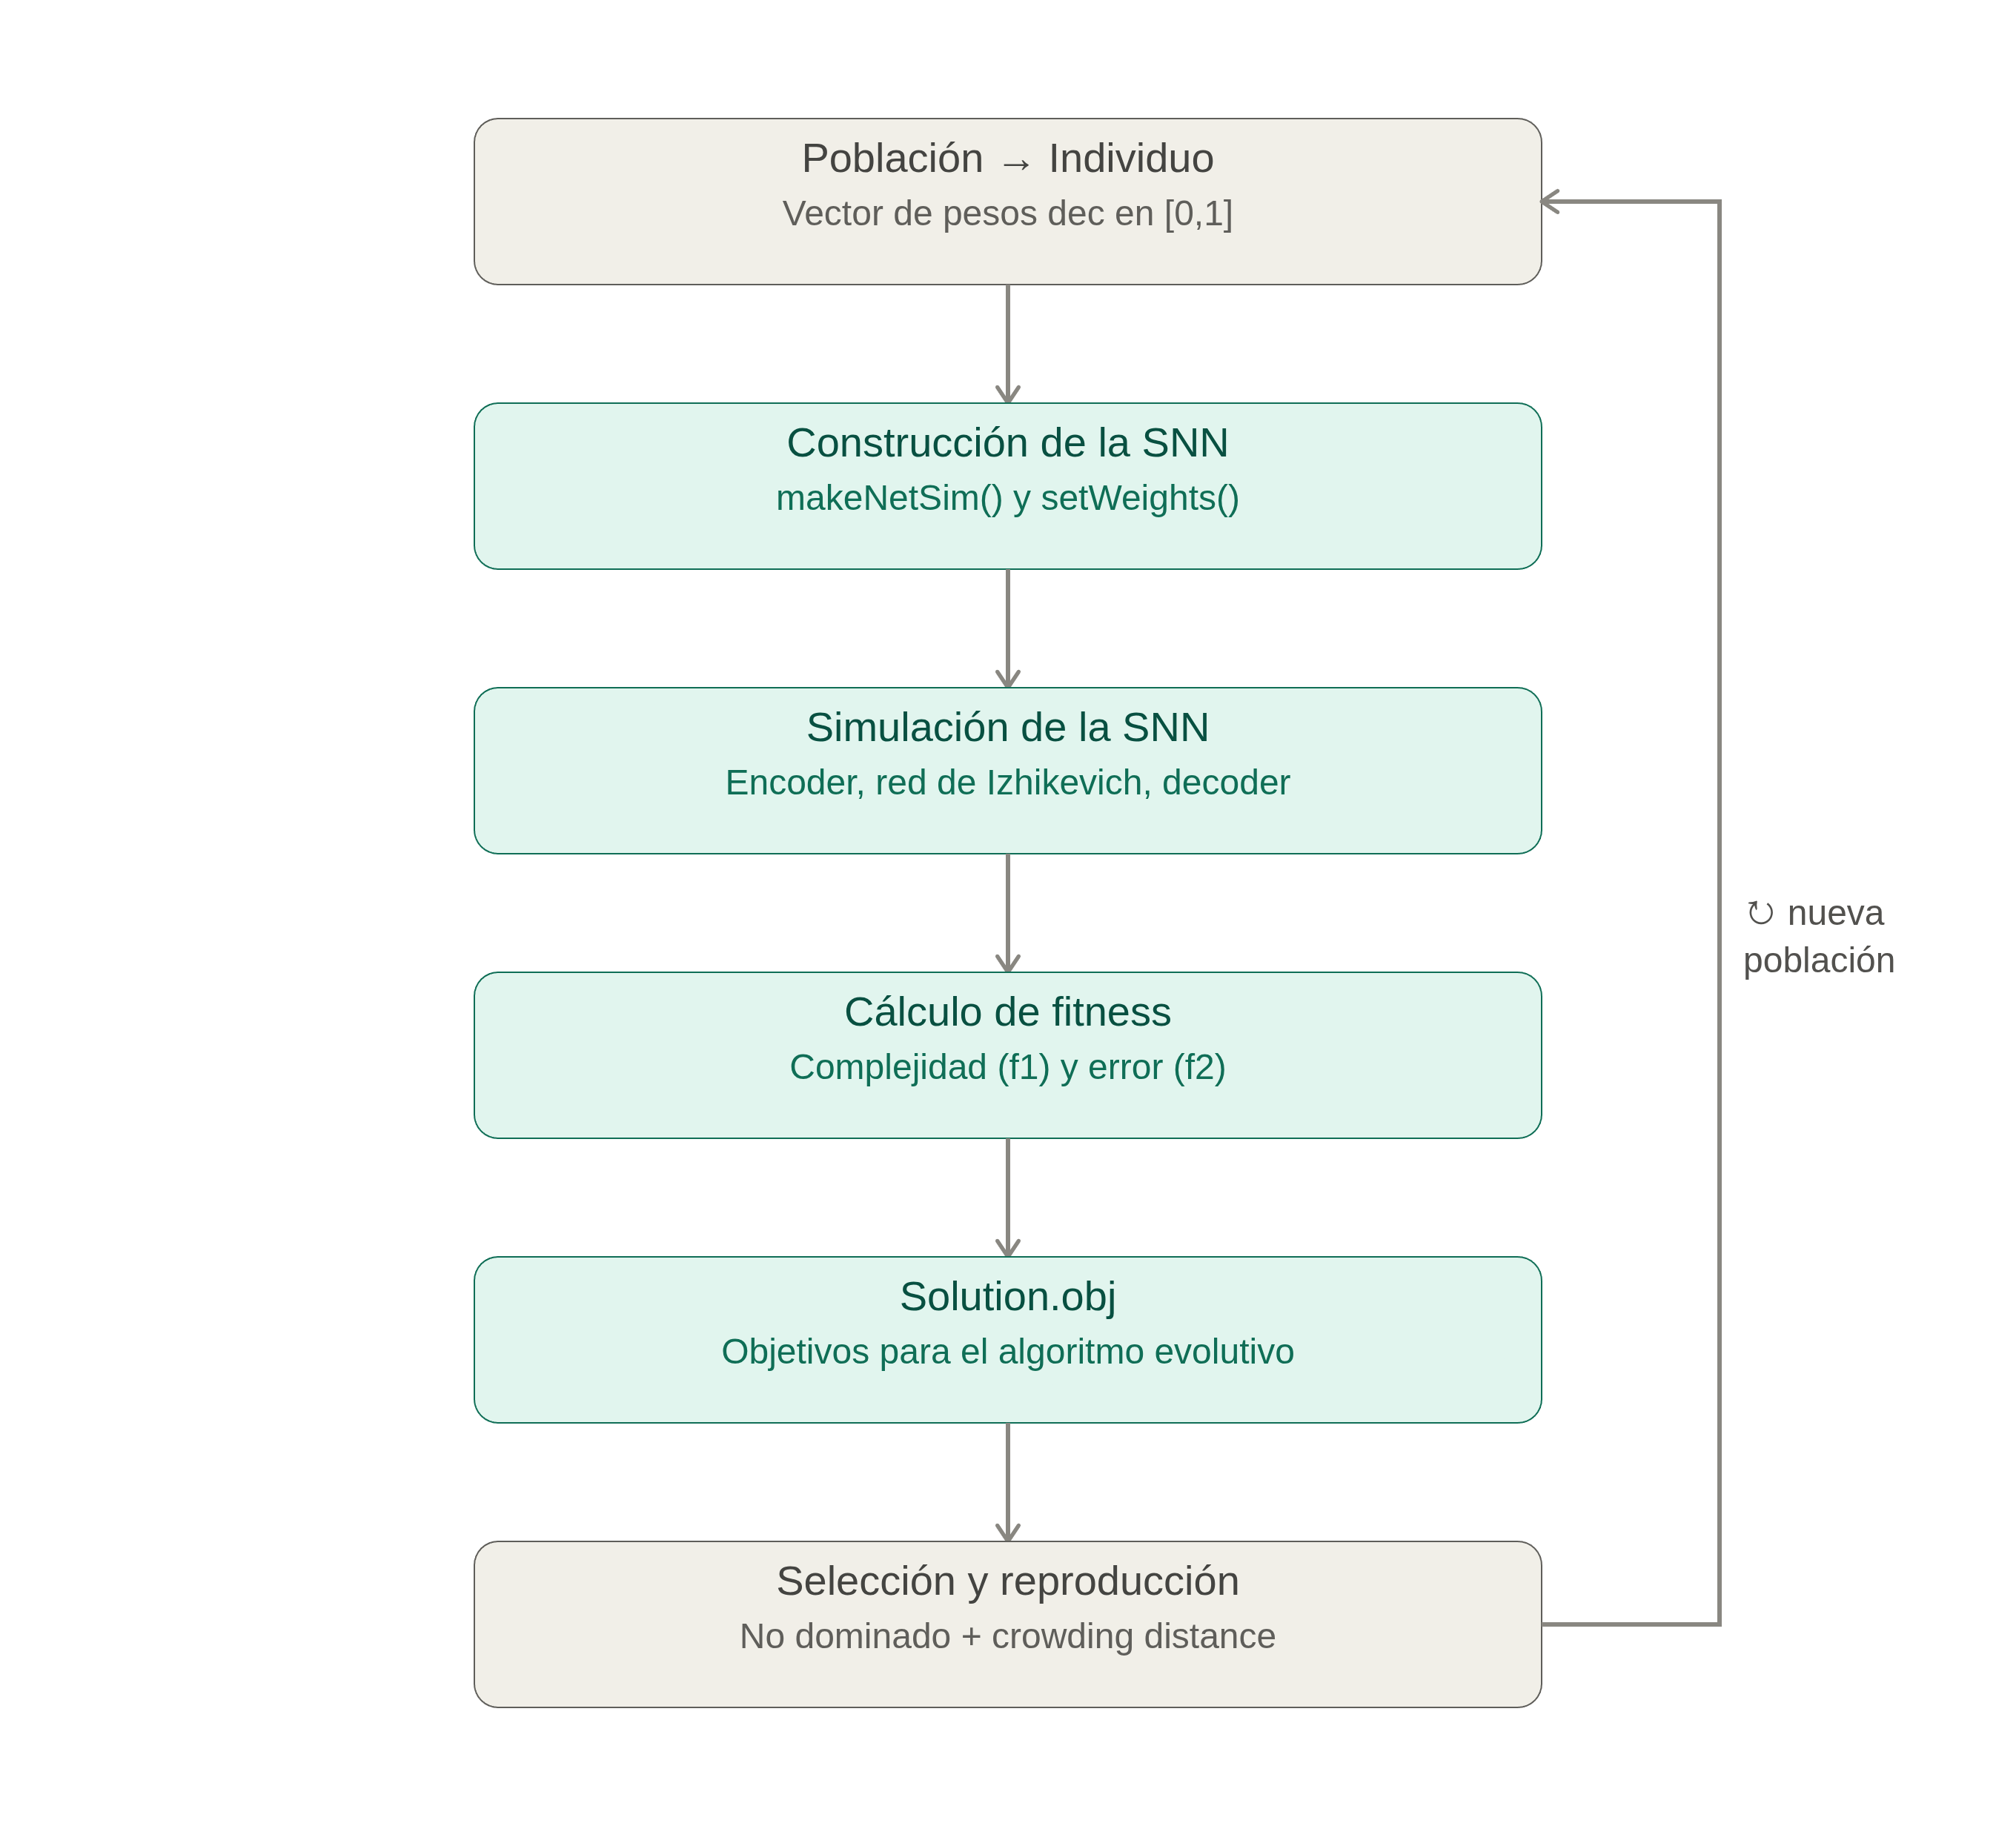
\includegraphics[width=0.75\linewidth]{images/pipeline_snn_evolutivo.png}
    \caption{Pipeline de evaluación del sistema evolutivo.}
    \label{fig:pipeline_snn_evo}
\end{figure}

\subsection{Flujo general de ejecución}
El ciclo evolutivo completo se instancia en el archivo principal del módulo evolutivo y sigue el patrón clásico población → inicialización → simulación/evaluación → selección → reproducción, repetido hasta agotar el presupuesto de evaluaciones. Este bucle define el flujo de información entre el módulo evolutivo y el simulador de SNN, garantizando tanto la coherencia de la evaluación multiobjetivo como la reproducibilidad de las corridas experimentales.

Durante la inicialización, se generan los pesos, produciendo aproximadamente un 50\% de ceros y sesgando la población inicial hacia redes esparsas. Sobre esta base común, cada algoritmo aplica una estrategia de arranque distinta: S-NSGA-II mediante VSSPS y MOEA-CKF mediante un Prior Analysis, ambas descritas en la Sección \ref{subsec:operadores_geneticos}.

En cada generación, todos los individuos se evalúan simulando la SNN sobre el conjunto de entrenamiento, en paralelo, aprovechando un pool de simuladores y redes preconstruidas por hilo. Una vez calculados los objetivos, ambos algoritmos utilizan selección por torneo binario para construir el mating pool\footnote{Conjunto de individuos seleccionados de la población actual para reproducirse.}, basada en el número de frente de Pareto y la distancia de aglomeración (\textit{crowding distance}), y posteriormente aplican selección ambiental tipo NSGA-II (ordenamiento no dominado + crowding) para decidir los individuos sobrevivientes tras fusionar padres e hijos. Esta etapa de selección es la única parte del ciclo generacional donde ambos algoritmos coinciden exactamente en su mecanismo.

La etapa de reproducción es, en cambio, donde S-NSGA-II y MOEA-CKF divergen con mayor fuerza, tal como se detalló en la Sección \ref{subsec:operadores_geneticos}. S-NSGA-II opera sobre un único vector real y aplica directamente sus operadores esparsos S-SBX y S-PM a todo el mating pool. MOEA-CKF, en cambio, divide la población en dos subgrupos en cada generación según la proporción $\rho$ y aplica a cada uno un procedimiento de reproducción distinto, guiado por reducción de dimensionalidad (PCA) y por agrupamiento de variables mediante \textit{k-means}, según se detalla en los pseudocódigos del Anexo \ref{chap:anexo-pseudo}.

El bucle generacional se ejecuta hasta que se alcanza el número máximo de evaluaciones \texttt{maxFE}; una vez terminada la evolución, se calcula el Hipervolumen (HV) del frente final y, opcionalmente, exporta el frente de Pareto, el historial de convergencia y los conteos de picos en el conjunto de test. El flujo general de ejecución, común en su estructura de alto nivel, pero con lógicas internas de inicialización y reproducción propias de cada algoritmo, se puede observar en la Figura \ref{fig:flujo_evo_511}.

\begin{figure}
    \centering
    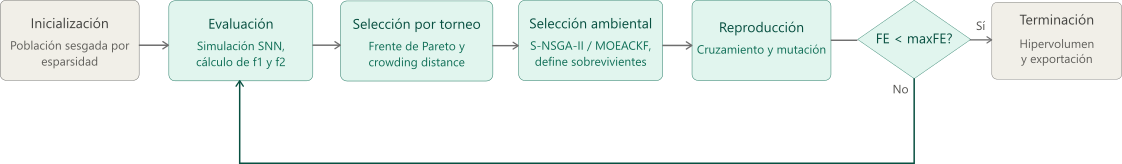
\includegraphics[width=1\linewidth]{images/flujo_evo_snn_horizontal.png}
    \caption{Flujo evolutivo generacional de alto nivel, común a ambos algoritmos en sus etapas de evaluación y selección. Las etapas de inicialización y reproducción encapsulan, bajo el mismo nombre, la lógica interna específica de S-NSGA-II y de MOEA-CKF. El ciclo repite evaluación mediante simulación de la SNN hasta que se cumple la condición de término $FE \geq maxFE$.}
    \label{fig:flujo_evo_511}
\end{figure}


\subsection{Módulos del sistema}
La implementación se organiza en torno a cinco módulos conceptuales que cubren la totalidad del pipeline: módulo evolutivo, simulador de SNN, manejo de datasets, métricas y configuración experimental. Esta separación en módulos permite mantener una arquitectura clara, donde el algoritmo evolutivo se mantiene independiente de los detalles del simulador y de la gestión de datos, facilitando la extensión y el análisis comparativo de algoritmos. Esta arquitectura modular se puede observar en la Figura \ref{fig:arquitectura_modular_sistema}.

El \textit{módulo evolutivo} define una jerarquía genérica Problema/Solución, implementa los dos algoritmos multiobjetivo y sus operadores genéticos. El \textit{simulador SNN} encapsula el modelo de neurona de Izhikevich, la estructura de la red (neuronas y sinapsis), el bucle de simulación temporal y los mecanismos de codificación y decodificación de spikes. A su vez, el \textit{módulo de datasets} se encarga de los archivos, la normalización, y la codificación de etiquetas. El \textit{módulo de métricas} las funciones objetivo y los indicadores agregados como el hipervolumen; finalmente, la \textit{configuración experimental} se gestiona íntegramente mediante scripts de orquestación.

\begin{figure}
    \centering
    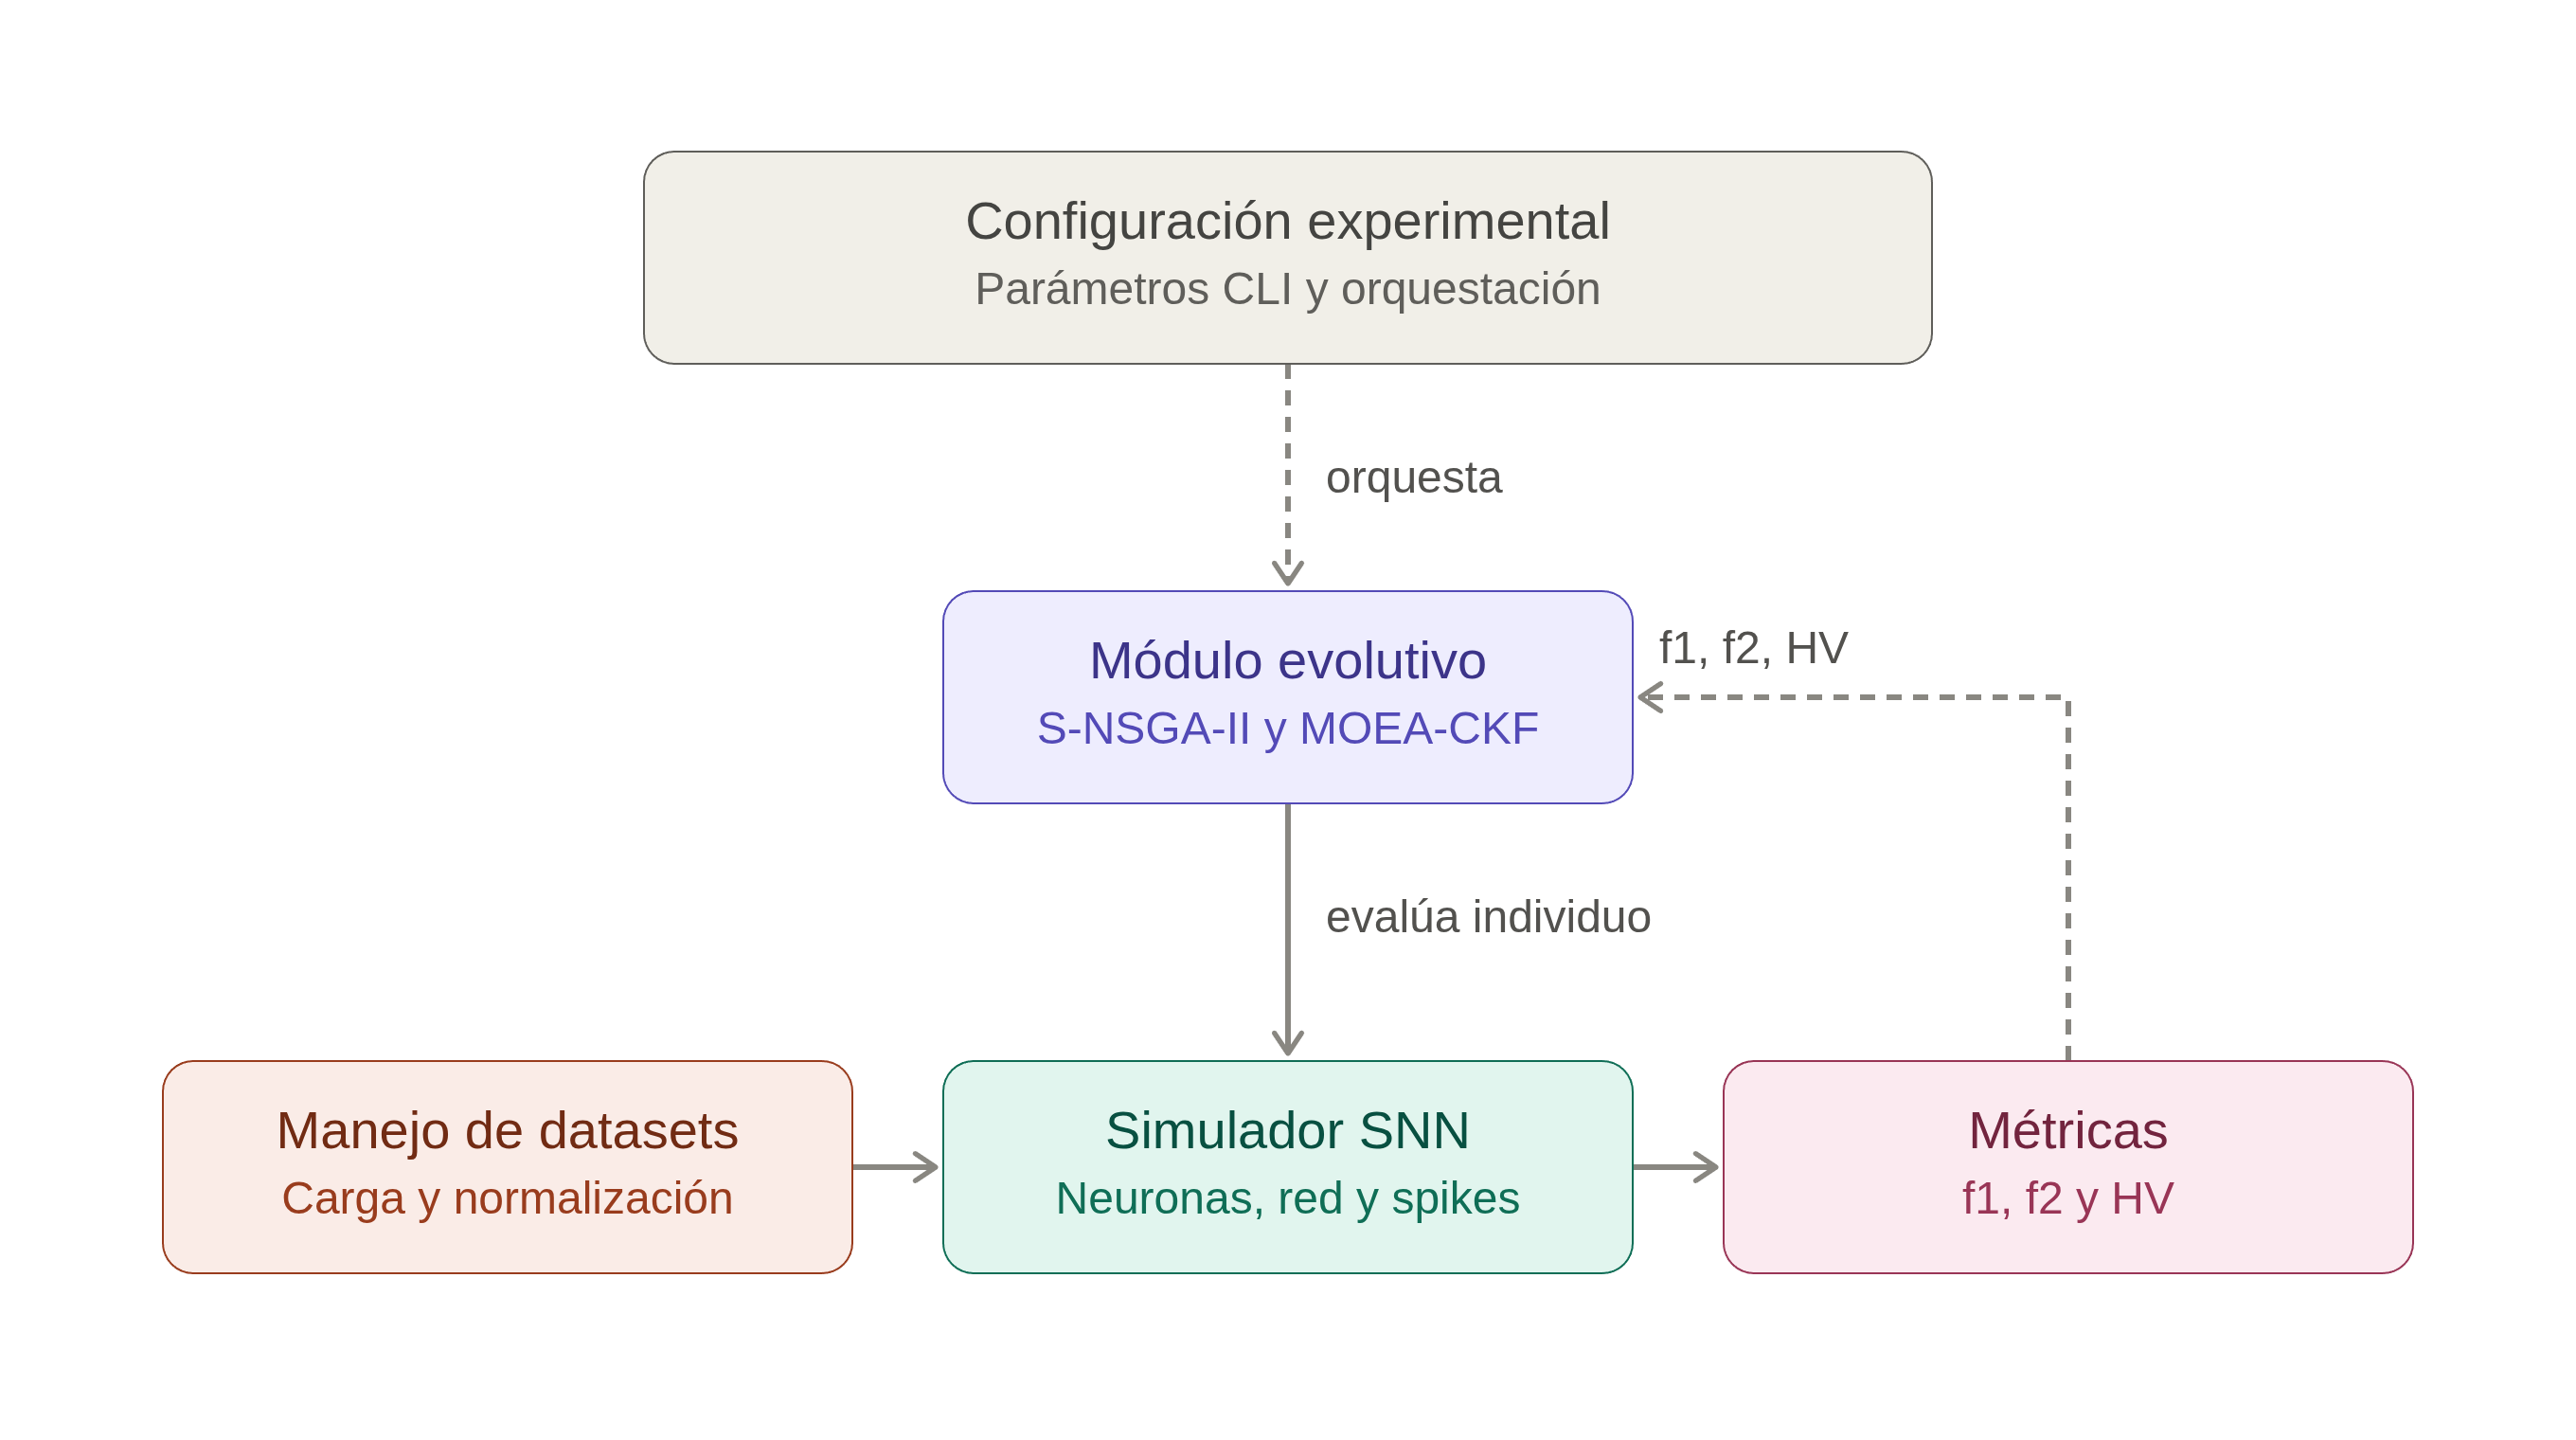
\includegraphics[width=0.7\linewidth]{images/modulos_sistema_snn.png}
    \caption{Arquitectura modular del sistema.}
    \label{fig:arquitectura_modular_sistema}
\end{figure}


%----------------------------

\section{Implementación de simulador SNN}\label{sec:simulador-snn}

El simulador SNN se implementó como un proyecto autónomo añadiendo además un framework de pruebas unitarias. La organización del código se estructura en módulos bien separados: núcleo de simulación (neurona, red, simulador), codificación de entrada, decodificación para clasificación y utilidades. Conceptualmente, la arquitectura sigue un pipeline Codificador → Red → Decodificador, donde un codificador transforma datos tabulares en trenes de espigas, la red de Izhikevich integra la dinámica neuronal y sináptica, y un decodificador de clasificación convierte los spikes de salida en decisiones y métricas de desempeño. El código fuente de este módulo está disponible como repositorio independiente en su repositorio: \url{https://github.com/Don-Uldaricio/snn-simulator}.

\subsection{Modelo neuronal y representación de la red}

Para esto, el simulador implementa exclusivamente neuronas de tipo Izhikevich, parametrizadas según el modelo original (ver \ref{sec:izhikevich}). La integración numérica se realiza mediante un esquema de Euler explícito con dos sub-pasos de tamaño $dt/2$ por paso de simulación, siguiendo la recomendación de Izhikevich para mejorar la estabilidad sin sacrificar eficiencia. La corriente total que recibe cada neurona combina conductancias excitatorias e inhibitorias con decaimiento exponencial, un término de corriente constante y un término de ruido uniforme generado con un RNG\footnote{Random Number Generator.}, lo que permite capturar variabilidad estocástica sin introducir condiciones de carrera.

Las conexiones sinápticas se representan mediante una estructura que almacena el índice de la neurona pre-sináptica, el índice de la neurona post-sináptica, una bandera que indica si la sinapsis es excitatoria o inhibitoria, y un peso escalar. A nivel de red, la topología se modela como una lista dispersa de sinapsis junto a listas de adyacencia pre-sinápticas y post-sinápticas (vectores de vectores de índices), lo que permite recorrer eficientemente las conexiones entrantes y salientes sin necesidad de matrices densas. El modelo no incorpora delays sinápticos explíctios ni conductancias por sinapsis: la transmisión de un spike es instantánea en el mismo paso de simulación y la dinámica de conductancias se implementa en las neuronas post-sinápticas.

\subsection{Motor de simulación y codificación}
El motor de simulación es la red, que mantiene vectores de neuronas Izhikevich y de sinapsis y ofrece métodos para avanzar la dinámica en el tiempo por pasos. En cada paso, el motor propaga las espigas generadas en el paso anterior actualizando las conductancias excitatorias e inhibitorias de las neuronas post-sinápticas, integra el estado de cada neurona y avanza el reloj global en un esquema de paso fijo, sin motor basado en eventos. El simulador envuelve a la red y a un codificador de entrada, gestionando la inyección de corrientes codificadas, la recolección de spikes y voltajes de salida, así como el cálculo de métricas como precisión, de modo que la simulación pueda utilizarse directamente como función objetivo en módulos externos de optimización. El módulo de codificación define dos implementaciones concretas: Poisson Encoder y TTFS (ver \ref{sec:codificacion-y-deco}).

\subsection{Validación y pruebas}
Se validó el simulador mediante una suite de 33 pruebas unitarias, implementadas con el framework Catch2 e integradas al sistema de compilación mediante CTest, lo que permite ejecutarlas de forma automatizada tras cada modificación del código fuente. Las pruebas se organizan según los mismos módulos conceptuales del simulador: núcleo, codificación y decodificación, tal como resume la Tabla \ref{tab:pruebas_simulador}.

\begin{table}[hbtp]
    \centering
    \small
    \caption{Distribución de las pruebas unitarias del simulador SNN por módulo.}
    \label{tab:pruebas_simulador}
    \begin{tabular}{lc}
        \toprule
        Módulo & N.º de pruebas \\
        \midrule
        Neurona (core/neuron) & 3 \\
        Red (core/network) & 7 \\
        Simulador (core/simulator) & 9 \\
        Codificación (encoding) & 9 \\
        Decodificación (decoding) & 5 \\
        \bottomrule
    \end{tabular}
\end{table}

En el núcleo, las pruebas sobre la neurona verificaron que una conductancia excitatoria sostenida produce disparos, que una conductancia inhibitoria de magnitud suficiente reduce el número de disparos respecto del caso puramente excitatorio, y que una corriente base constante ($i_{\text{offset}}$) es capaz de inducir disparos sin necesidad de estímulo externo. Sobre la red, las pruebas comprobaron la construcción correcta de la topología (conteo de neuronas, sinapsis, entradas y salidas), el almacenamiento y el peso de cada sinapsis, incluyendo asignación individual, masiva y homogénea, y la propagación efectiva de espigas a través de sinapsis excitatorias e inhibitorias en una red mínima de dos neuronas.

Sobre el simulador se probaron tanto la simulación con corriente directa (silencio total con corriente nula, disparos con corriente alta, y una entrada de tiempos de disparo por cada neurona de salida en el resultado) como la simulación con codificación de entrada, verificando que valores de entrada más altos producen más espigas en la salida. También se validaron las mutaciones de topología empleadas por los algoritmos evolutivos como inserción y eliminación de neuronas.

En codificación se probaron los dos esquemas implementados. El codificador de Poisson se validó verificando que un valor de entrada nulo no generaba espigas, que un valor alto generaba consistentemente al menos una espiga, que valores más altos producían más espigas que valores bajos bajo una ventana temporal, y que todos los tiempos de espiga generados caen dentro de la ventana de codificación. El codificador TTFS se validó comprobando que valores de entrada más altos generaban una espiga más temprana que valores bajos, y que un valor por debajo del umbral configurado no generaba espiga alguna.

En decodificación se probó unitariamente que el decodificador de clasificación seleccionaba la neurona de salida con mayor cantidad de espigas, que ante un empate en el conteo de espigas elegía una clase al azar entre las empatadas, y que normalizaba los puntajes por clase al intervalo $[0,1]$. Finalmente, se incluyen dos pruebas de integración extremo a extremo que combinan el Simulador y el Decodificador: una evalúa la exactitud de clasificación sobre un conjunto sintético de trece muestras con dos clases separables, exigiendo una exactitud mínima de 80\%, y otra evalúa la consistencia estadística de sobre diez repeticiones de una misma muestra codificada de forma estocástica, exigiendo que al menos ocho de diez repeticiones acierten la clase correcta.

Dado que los codificadores de Poisson y de tasa son estocásticos, varias pruebas emplean ventanas temporales prolongadas (hasta 500 ms) o repeticiones múltiples (10 corridas) para reducir la probabilidad de falsos negativos por variabilidad aleatoria, en lugar de fijar una semilla determinista para el generador de números aleatorios.

%  \subsection{Decisiones de diseño y evolución}
% Un aspecto central del diseño es que el simulador no implementa reglas de plasticidad internas como STDP, \textit{backpropagation through time} o gradientes sustitutos: la dinámica neuronal y sináptica es puramente forward, y el ajuste de pesos se delega expresamente al módulo externo de optimización evolutiva multiobjetivo, que utiliza el simulador como librería estática. Esta separación de responsabilidades permite mantener el simulador SNN pequeño, testeable y enfocado en la fidelidad de la dinámica de disparo, mientras que la exploración del espacio de pesos y topologías se aborda en un código independiente descrito en el capítulo dedicado a la optimización evolutiva.

%----------------------------------------------

\section{Implementación de algoritmos evolutivos}\label{sec:algoritmos-evolutivos}
Para la implementación de los algoritmos evolutivos aplicado al entrenamiento de SNN, se realizó la migración de los algoritmos desde la plataforma PlatEMO \cite{8065138_platEMO} a C++, cuya versión original se encuentra desarrollada en MATLAB. La migración se llevó a cabo procurando conservar la lógica original de las estructuras principales del código, incluyendo la representación de individuos, la inicialización de la población, los operadores genéticos, los mecanismos de selección y el procedimiento de actualización generacional. En aquellos casos en que ciertas funciones o utilidades de MATLAB no contaban con un equivalente directo en C++, se desarrollaron implementaciones alternativas que mantuvieran un comportamiento funcionalmente equivalente dentro del algoritmo. Estos casos correspondieron principalmente a funciones nativas o de \textit{toolbox} de MATLAB sin contraparte en la biblioteca estándar de C++ ni en Eigen (\texttt{unique(...,'rows')}, \texttt{sortrows}, \texttt{pdist2} o \texttt{kmeans}) y a las funciones de generación de números aleatorios (\texttt{randi}, \texttt{randperm}, \texttt{unifrnd}), cuyo generador difiere entre ambas plataformas. La Tabla \ref{tab:funciones_sin_equivalente} detalla estos casos y la estrategia de reimplementación adoptada en cada uno. En la Tabla \ref{tab:fidelidad_algoritmos} se muestra un resumen de la fidelidad de la migración de los SMOEA a C++. El código fuente de este módulo está disponible como repositorio independiente (ver Anexo \ref{chap:anexo-repos}).

% En este caso, S-NSGA-II corresponde al algoritmo con mayor fidelidad respecto de la implementación original, debido a que sus operadores presentan una lógica más directa de traducir que los componentes de MOEA-CKF.

Dado que MATLAB y C++ implementan generadores de números pseudoaleatorios distintos, no fue posible reproducir de forma idéntica, número a número, la traza de ejecución de un algoritmo estocástico entre ambas implementaciones. Por esta razón, la equivalencia entre las versiones MATLAB y C++ de cada operador no se validó comparando las salidas numéricas de ejecuciones específicas, sino a nivel de la construcción matemática y algorítmica de cada componente: se verificó que cada función migrada implementara la misma definición matemática, el mismo criterio de orden lexicográfico, o el mismo procedimiento discreto que su contraparte original (por ejemplo, el muestreo uniforme con o sin reemplazo de \texttt{randperm}/\texttt{randi}). Esta fue, por tanto, una validación de equivalencia funcional por construcción y no una validación empírica de igualdad de resultados entre plataformas, lo cual se reconoce como una limitación metodológica del proceso de migración.

Con el fin de facilitar la mantenibilidad y la validación del sistema, la implementación se organizó de forma modular al igual que en el código original. Se separaron los componentes asociados a la codificación de soluciones, los operadores genéticos, la evaluación del desempeño de la población y la interfaz de comunicación con el simulador de SNN. Esta organización permitió desacoplar la lógica propia de cada algoritmo evolutivo de la lógica de simulación neuronal, favoreciendo la reutilización de componentes en distintas configuraciones experimentales. La Figura \ref{fig:modulos_platemo_cpp} muestra esta organización interna del módulo evolutivo.

\begin{figure}[hbtp]
    \centering
    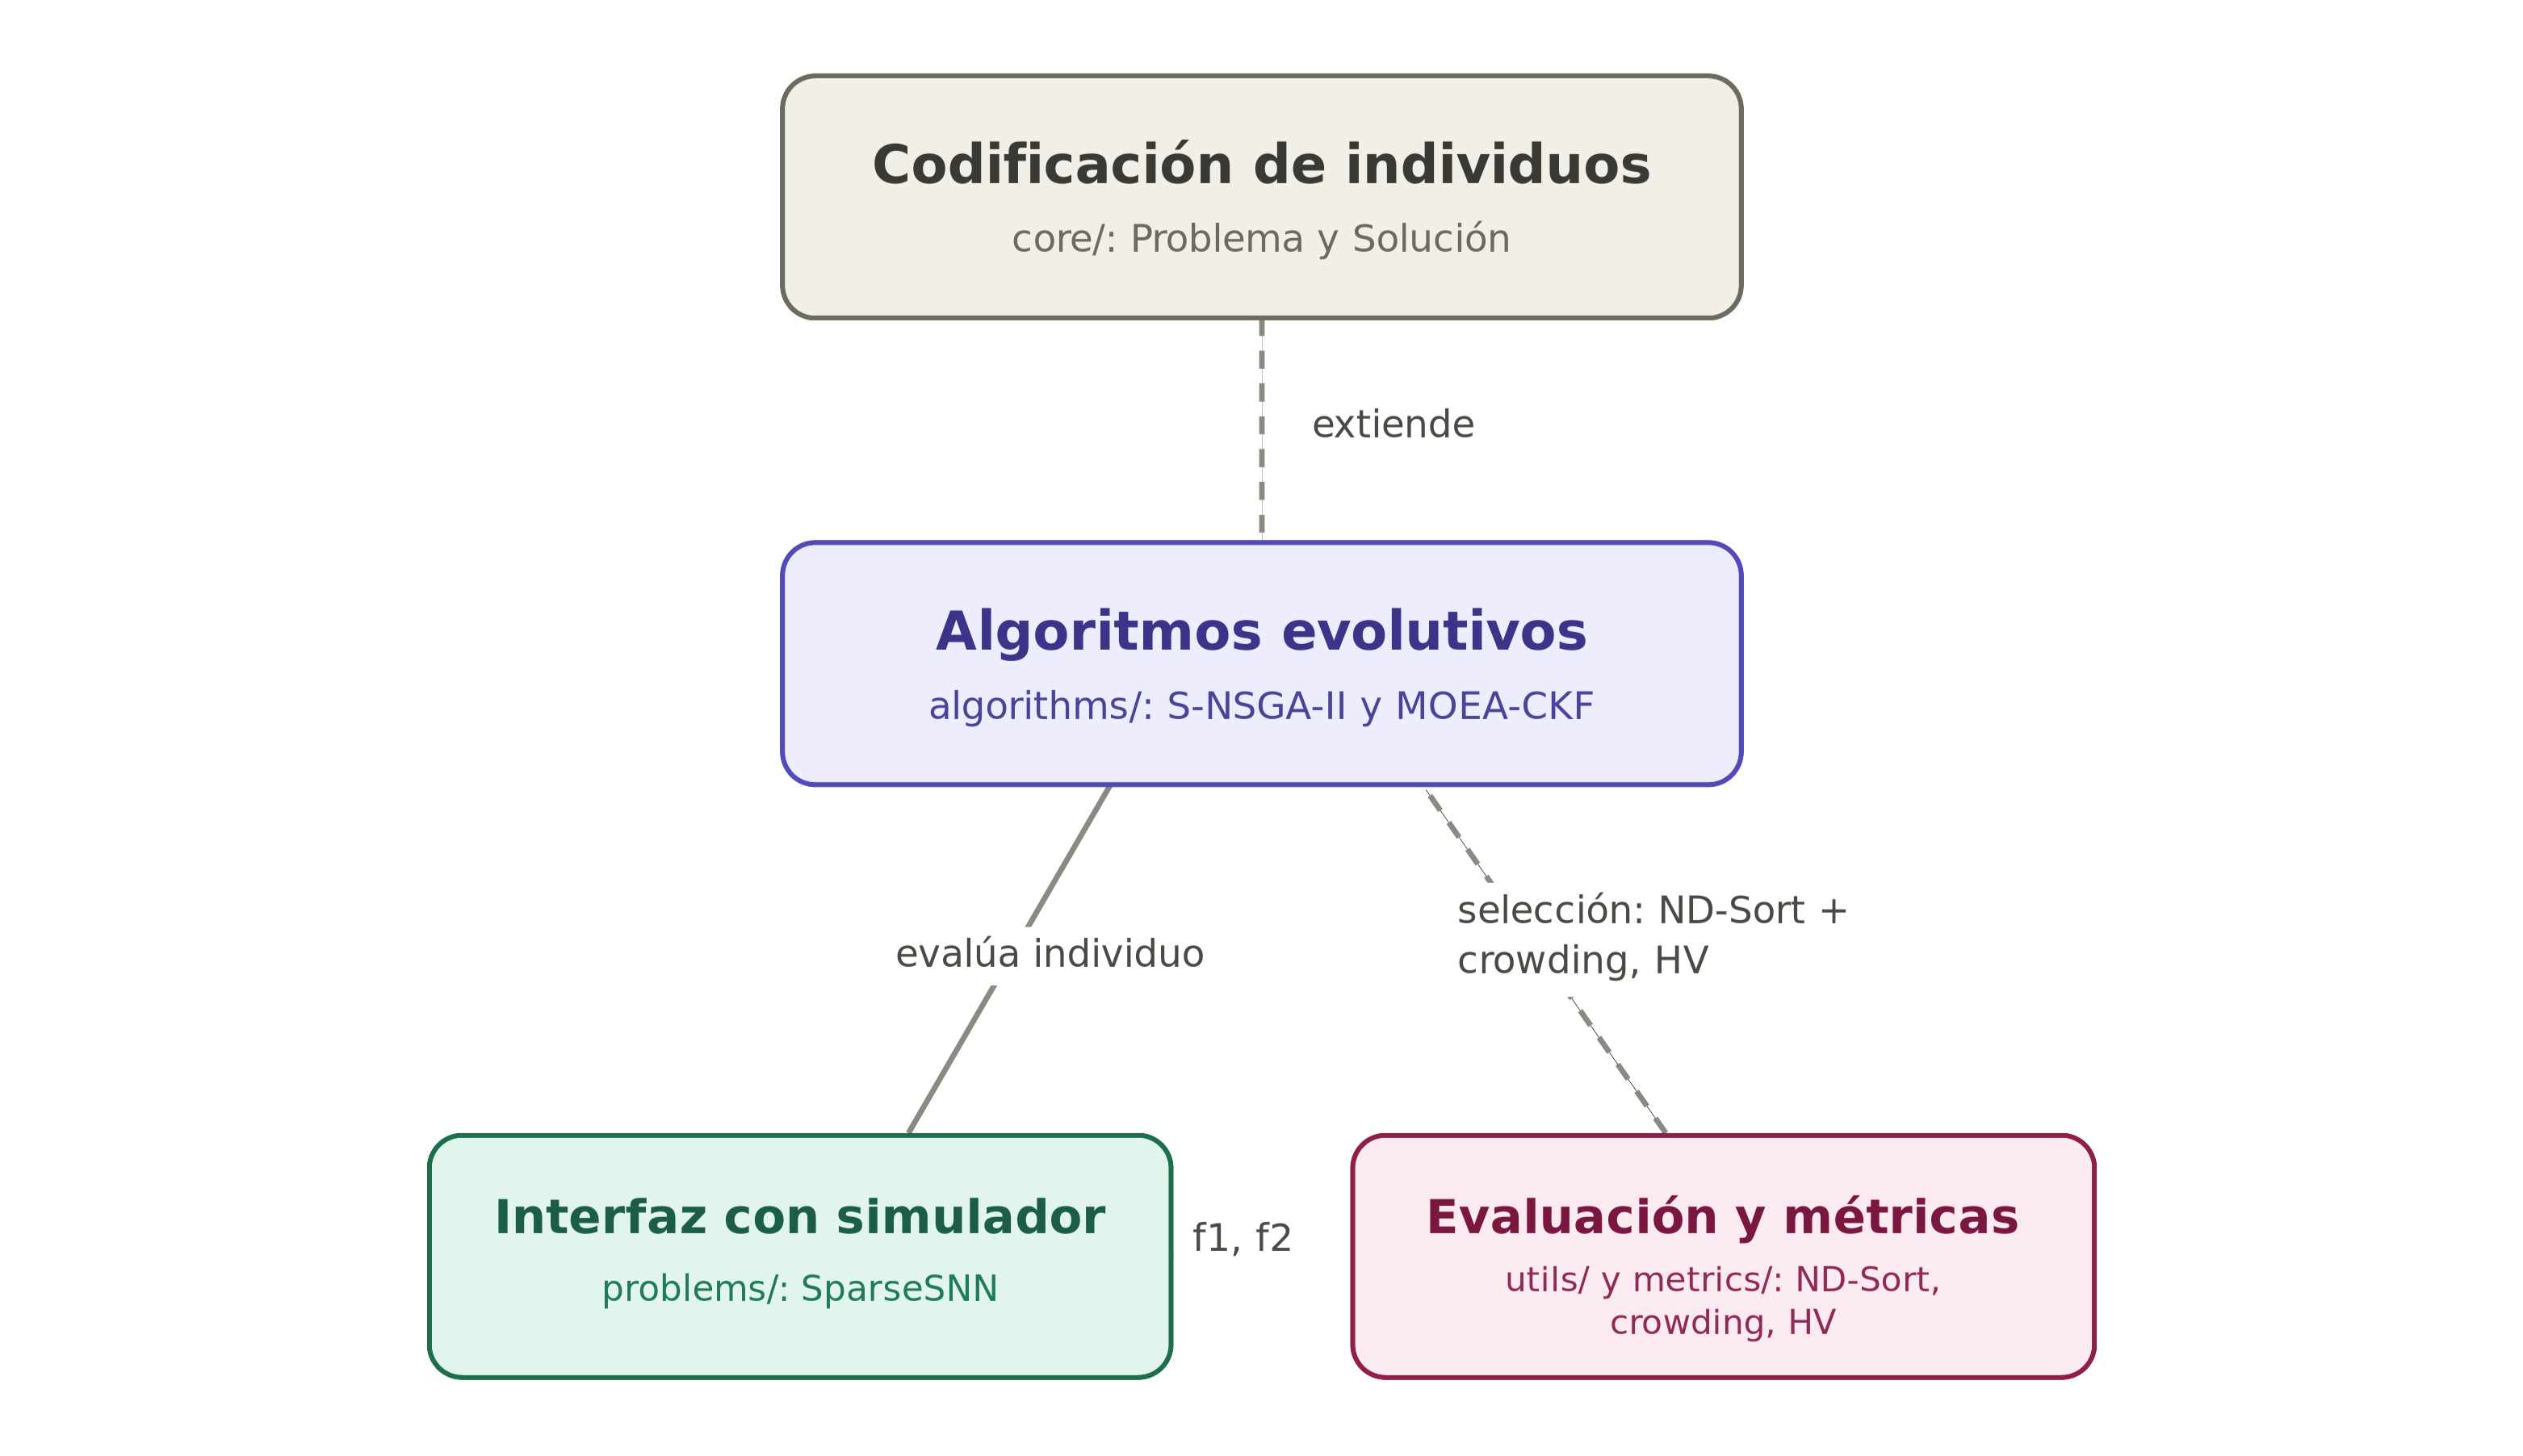
\includegraphics[width=0.75\linewidth]{images/modulos_algoritmos_evolutivos.png}
    \caption{Organización modular del módulo evolutivo.}
    \label{fig:modulos_platemo_cpp}
\end{figure}

La representación de cada individuo consistió en un vector real de pesos sinápticos definidos sobre la topología fija descrita en la Sección \ref{sec:arqui_sistema}. Dado que un peso nulo desactiva efectivamente una sinapsis, el mismo vector codificó implícitamente tanto la presencia o ausencia de cada conexión como la intensidad de las conexiones activas, permitiendo abordar el problema desde un enfoque neuroevolutivo sin requerir un cromosoma de topología independiente. Esta codificación conjunta fue la que permitió optimizar simultáneamente el desempeño de clasificación y la complejidad estructural de la red, los dos objetivos definidos para el problema.

Una vez implementados los algoritmos en C++, estos fueron integrados con el simulador de SNN a través del problema de entrenamiento de SNN. Así, la evaluación de cada individuo consistió en ejecutar una configuración experimental completa definida por un dataset, una cantidad de variables de entrada y un número determinado de neuronas en la capa oculta. Bajo este esquema, cada solución propuesta por el algoritmo evolutivo fue decodificada en una arquitectura de red concreta, simulada sobre los datos correspondientes y evaluada según las funciones objetivo definidas para el problema. Con esto se obtuvo una plataforma experimental unificada, capaz de conectar el proceso evolutivo con la simulación de SNN y de soportar las etapas posteriores de evaluación y comparación de resultados. El proceso de optimización siguió un ciclo iterativo que ya fue explicado en la Sección \ref{sec:arqui_sistema}.

% Finalmente, se verificó que la implementación en C++ preservara la lógica general de los algoritmos de referencia y resultara compatible con la ejecución repetible de experimentos. Para ello, se incorporaron mecanismos de parametrización de los algoritmos, configuración del tamaño de la capa oculta y gestión del dataset a utilizar en cada ejecución. 


%----------------------------

    \chapter{Resultados}\label{chapter:resultados}

\section{Selección del framework de simulación SNN}
\label{sec:benchmark-framework-resultados}

En esta sección se presentan los resultados cuantitativos utilizados para comparar los frameworks \textit{ANNarchy}, \textit{NEST} y \textit{snn-simulator}, siguiendo el diseño experimental y el plan de análisis descritos en \ref{sec:benchmark-framework-metodologia}.

\paragraph{Tiempo de evaluación y comparación estadística}

La Figura~\ref{fig:eval-time-frameworks} muestra los resultados del tiempo de evaluación de la función objetivo para cada combinación de configuración y framework con 30 repeticiones en todas las configuraciones. Los resultados en detalle se encuentran en la Tabla \ref{tab:framework-evals-res}.

\begin{figure}
    \centering
    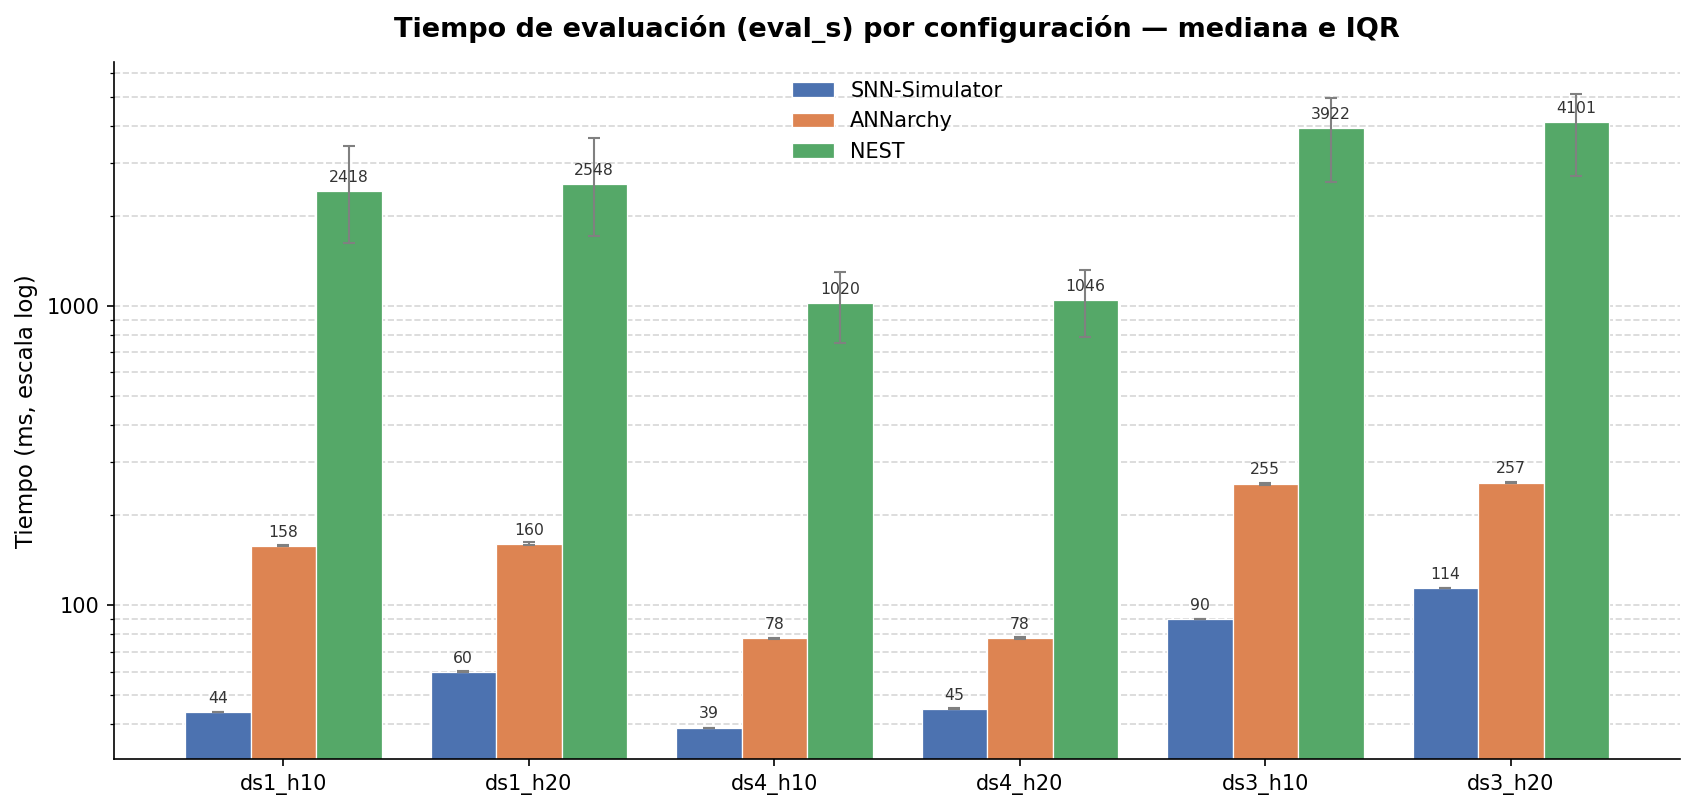
\includegraphics[width=0.8\linewidth]{images/plot_eval_s_median_iqr.png}
    \caption{Tiempo de evaluación por configuración y framework.}
    \label{fig:eval-time-frameworks}
\end{figure}

% En las seis configuraciones probadas se mantuvo el orden \textit{snn-simulator} \(<\) ANNarchy \(<\) NEST. Ordenando las seis configuraciones por dimensionalidad $D$, el ratio de velocidad \textit{snn-simulator} vs. cada competidor decrece de forma monótona: frente a ANNarchy, va de 3.58x (\texttt{ds1\_h10}, $D=160$) a 1.72x (\texttt{ds4\_h20}, $D=1240$); frente a NEST, de 54.9x ($D=160$) a 23.2x ($D=1240$). El patrón se sostuvo tanto al aumentar el número de neuronas en la capa oculta (de 10 a 20 neuronas dentro del mismo dataset) como al aumentar el número de características (mismo \texttt{nHidden}, distinto dataset), sin que este benchmark mostrara cuál de las dos dimensiones pesa más. Para el rango de $D$ efectivamente usado en esta prueba, \textit{snn-simulator} nunca deja de ser la opción más rápida por un margen amplio. Sin embargo, extrapolar la ventaja observada aquí a dimensiones muy superiores no está garantizado por estos datos.

% Ordenando las seis configuraciones por dimensionalidad $D$, el ratio de medianas de \textit{snn-simulator} frente a cada competidor decrece de forma monótona: frente a ANNarchy, va de 3.58x (\texttt{ds1\_h10}, $D=160$) a 1.72x (\texttt{ds4\_h20}, $D=1240$); frente a NEST, de 54.9x ($D=160$) a 23.2x ($D=1240$).

En las seis configuraciones probadas se mantuvo el mismo orden en tiempo de ejecución: \textit{snn-simulator} \(<\) ANNarchy \(<\) NEST. El patrón se sostuvo tanto al aumentar el número de neuronas en la capa oculta (de 10 a 20 neuronas dentro del mismo dataset) como al aumentar el número de características, sin que este benchmark mostrara cuál de las dos dimensiones pesa más. Se reporta la mediana debido al uso de la prueba no paramétrica de Mann-Whitney U. Para el rango de $D$ efectivamente usado en esta prueba, \textit{snn-simulator} nunca deja de ser la opción más rápida por un margen amplio. Sin embargo, extrapolar la ventaja observada aquí a dimensiones muy superiores no está garantizado por estos datos.


% \subsection{Comparación estadística entre frameworks (Mann-Whitney U)}

La Tabla~\ref{tab:framework-mannwhitney-res} resume las diferencias entre \textit{snn-simulator} y cada competidor, en base a la mediana, junto con el valor \(p\) de la prueba Mann-Whitney U, con 30 ejecuciones. Las 18 comparaciones por pares (tres frameworks por seis configuraciones) arrojan \(U = 0\) y separación total de las distribuciones, con \(p \approx 3{.}0 \times 10^{-11}\) en todos los casos. La comparación ANNarchy frente a NEST, no mostrada en la tabla, también resulta significativa a favor de ANNarchy en todas las configuraciones.

\begin{table}[htbp]
\centering
\small
\caption{Comparaciones por pares mediante Mann-Whitney \(U\). Las diferencias corresponden a la mediana de \textit{snn-simulator} menos la del competidor.}
\label{tab:framework-mannwhitney-res}
\begin{tabular}{lrrrr}
\toprule
Config & $\Delta$ vs ANNarchy (ms) & $p$ & $\Delta$ vs NEST (ms) & $p$ \\
\midrule
ds1\_h10 & -113.85 & $<0.0001$ & -2374.07 & $<0.0001$ \\
ds1\_h20 & -100.13 & $<0.0001$ & -2487.99 & $<0.0001$ \\
ds4\_h10 &  -38.47 & $<0.0001$ &  -980.50 & $<0.0001$ \\
ds4\_h20 &  -32.41 & $<0.0001$ & -1001.07 & $<0.0001$ \\
ds3\_h10 & -165.10 & $<0.0001$ & -3832.01 & $<0.0001$ \\
ds3\_h20 & -142.74 & $<0.0001$ & -3986.35 & $<0.0001$ \\
\bottomrule
\end{tabular}
\end{table}

El \textit{p-valor} indica que la diferencia no es producto del azar, pero no cuantifica qué tan grande es. De las 900 comparaciones posibles entre una medición de \textit{snn-simulator} y una del competidor ($30\times30$), \textit{snn-simulator} fue menor en las 900, sin un solo caso de solapamiento. No es un caso límite cercano a $p=0.05$, sino una diferencia que se sostiene en el 100\% de las 18 comparaciones. %(3 pares × 6 configs).

\paragraph{Tiempo de construcción y escalabilidad de la red}

La Figura \ref{fig:build_s_by_config} muestra el tiempo de construcción de la red por cada framework en las seis configuraciones con 30 repeticiones en cada una. El \textit{snn-simulator} construye la red en microsegundos, entre tres y cuatro órdenes de magnitud más rápido que NEST y ANNarchy. ANNarchy incurre además en un costo adicional de compilación Cython de aproximadamente 9{.}6–9{.}8 segundos por corrida. Los resultados completos se pueden visualizar en la Tabla \ref{tab:framework-build-memory-res} del Anexo.

\begin{figure}
    \centering
    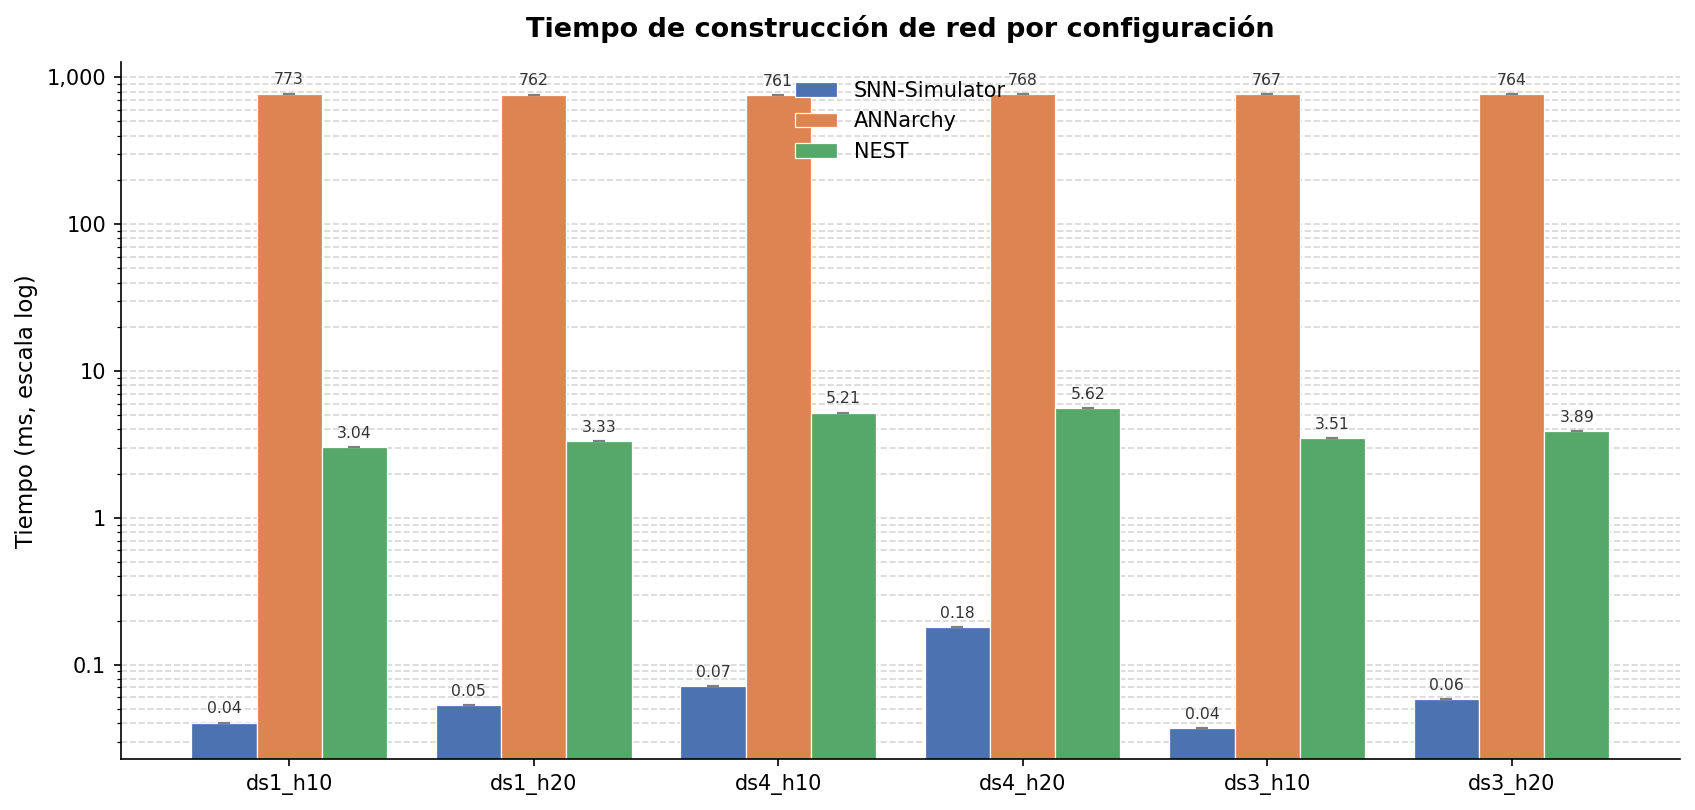
\includegraphics[width=0.8\linewidth]{images/plot_build_s_by_config.png}
    \caption{Tiempo de construcción por configuración y framework.}
    \label{fig:build_s_by_config}
\end{figure}

% \subsection{Overhead puro del algoritmo evolutivo}

% La Tabla~\ref{tab:framework-moea-overhead-res} resume el tiempo de ejecución de MOEA-CKF y S-NSGA-II sin simulador real (problema trivial), junto con la razón entre ambos.

% \begin{table}[htbp]
% \centering
% \small
% \caption{Overhead de los algoritmos evolutivos sin simulador.}
% \label{tab:framework-moea-overhead-res}
% \begin{tabular}{lrrrr}
% \toprule
% Config & $D$ & MOEACKF (s) & SNSGAII (s) & Razón MOEACKF/SNSGAII \\
% \midrule
% ds1\_h10 & 160  &  4.18 & 0.082 &  51.1$\times$ \\
% ds1\_h20 & 320  & 17.57 & 0.143 & 123.2$\times$ \\
% ds4\_h10 & 620  & 82.26 & 0.255 & 322.3$\times$ \\
% ds4\_h20 & 1240 & 222.19 & 0.503 & 442.1$\times$ \\
% ds3\_h10 & 260  & 12.39 & 0.121 & 102.4$\times$ \\
% ds3\_h20 & 520  & 61.25 & 0.215 & 284.4$\times$ \\
% \bottomrule
% \end{tabular}
% \end{table}

% MOEA-CKF escala mucho peor con la dimensionalidad \(D\) del vector de pesos que S-NSGA-II, y este overhead se suma al costo de simulación independientemente del framework elegido.

\paragraph{Selección del framework}

Con base en los resultados anteriores, se selecciona \textit{snn-simulator} como framework de simulación SNN para el pipeline de entrenamiento. La decisión se apoya en: (i) tiempos de evaluación significativamente menores en las seis configuraciones, con separación completa de las distribuciones frente a ANNarchy y NEST, y (ii) tiempos de construcción varios órdenes de magnitud inferiores sin compilación adicional.

La principal desventaja de \textit{snn-simulator} es un consumo de memoria aproximadamente 9 MB superior al de ANNarchy en las configuraciones evaluadas, siendo esta diferencia irrelevante frente a la ventaja temporal de dos a tres órdenes de magnitud y frente al hecho de que la memoria de \textit{snn-simulator} se mantiene estable mientras que la de NEST crece con el número de evaluaciones.

Las amenazas a la validez incluyen la anomalía confirmada de tendencia en NEST (crecimiento monótono del tiempo de evaluación al duplicar el número de repeticiones dentro del mismo proceso), y la realización de mediciones en una sola máquina y sesión diferente a donde se realizaron los experimentos finales.


%---------------

\section{Resultados de la búsqueda de hiperparámetros}

Siguiendo la metodología descrita en la Sección~\ref{sec:metodologia_busqueda_hiper}, se ejecutaron ocho estudios independientes de búsqueda de hiperparámetros, uno por cada algoritmo sobre los datasets seleccionados.

La Tabla \ref{tab:hv_por_dataset_resultados} resume el HV medio de la mejor configuración encontrada en cada estudio, junto con el \emph{trial} ganador y la arquitectura asociada. En todos los casos, la configuración ganadora corresponde a redes con dos neuronas de salida con codificación Poisson o TTFS según el dataset y el algoritmo.

% Please add the following required packages to your document preamble:
% \usepackage{multirow}
\begin{table}[htbp]
\centering
\small
\caption{Mejor HV medio, promediado sobre configuraciones de 20, 40 y 80 neuronas, por algoritmo y conjunto de datos. La arquitectura es la seleccionada mediante la búsqueda de hiperparámetros.}
\label{tab:hv_por_dataset_resultados}
\begin{tabular}{ccclccl}
\hline
\textbf{Dataset}            & \textbf{Características}     & \textbf{maxFE}                    & \textbf{Algoritmo} & \textbf{HV medio} & \textbf{Trial}& \textbf{Arquitectura} \\ \hline
\multirow{2}{*}{1} & \multirow{2}{*}{14} & \multirow{2}{*}{9\,900}  & MOEA-CKF  & 0.8707   & 50    & Poisson             \\
                   &                     &                          & S-NSGA-II & 0.8742   & 17    & TTFS                \\ \hline
\multirow{2}{*}{2} & \multirow{2}{*}{18} & \multirow{2}{*}{11\,500} & MOEA-CKF  & 0.9297   & 31    & TTFS                \\
                   &                     &                          & S-NSGA-II & 0.9291   & 44    & Poisson             \\ \hline
\multirow{2}{*}{3} & \multirow{2}{*}{24} & \multirow{2}{*}{13\,900} & MOEA-CKF  & 0.7501   & 40    & TTFS                \\
                   &                     &                          & S-NSGA-II & 0.7550   & 24    & Poisson             \\ \hline
\multirow{2}{*}{4} & \multirow{2}{*}{60} & \multirow{2}{*}{28\,300} & MOEA-CKF  & 0.8008   & 59    & TTFS                \\
                   &                     &                          & S-NSGA-II & 0.8268   & 11    & TTFS   \\ \hline
\end{tabular}
\end{table}

\subsection{Resultados por dataset}

\subsubsection{Dataset 1: Statlog Australian}

Ambos algoritmos alcanzan un HV medio muy similar en sus mejores configuraciones: 0.8707 para MOEA-CKF y 0.8742 para S-NSGA-II. La diferencia principal es el codificador, Poisson en MOEA-CKF y TTFS en S-NSGA-II. Estas configuraciones se detallan en la Tabla~\ref{tab:hiper_mejor_config}, donde se observa además que los índices de distribución de cruce y mutación, así como los parámetros de esparsidad, adoptan valores distintos entre algoritmos.

\begin{table}[htbp]
    \centering
    \small
    \caption{Hiperparámetros de la mejor configuración por algoritmo y dataset.}
    \label{tab:hiper_mejor_config}
    \resizebox{\textwidth}{!}{%
        \begin{tabular}{lcccccccc}
            \hline
            Parámetro &
            ds1-CKF &
            ds1-NSGA &
            ds2-CKF &
            ds2-NSGA &
            ds3-CKF &
            ds3-NSGA &
            ds4-CKF &
            ds4-NSGA \\
            \hline
            disC   & 28.01 & 16.61 & 9.90  & 5.03  & 99.85 & 9.84  & 74.56 & 6.01  \\
            disM   & 28.35 & 9.55  & 8.04  & 50.62 & 21.35 & 8.14  & 5.66  & 56.64 \\
            proM   & 1.79  & 2.99  & 2.07  & 2.90  & 0.74  & 2.44  & 0.58  & 1.66  \\
            disSM  & 25.44 & 35.44 & 18.60 & 61.71 & 6.00  & 63.25 & 6.49  & 82.44 \\
            proSM  & 1.02  & 1.69  & 2.34  & 1.49  & 1.21  & 0.99  & 1.47  & 2.67  \\
            sLower & 0.81  & 0.66  & 0.54  & 0.85  & 0.88  & 0.69  & 0.70  & 0.63  \\
            sGap   & 0.12  & 0.23  & 0.26  & 0.30  & 0.25  & 0.27  & 0.07  & 0.05  \\
            wScale & 34.75 & 13.63 & 8.99  & 44.41 & 36.96 & 16.42 & 27.12 & 40.27 \\
            \hline
        \end{tabular}%
    }
\end{table}

Las trayectorias de convergencia del HV medio por \emph{trial} muestran que ambos estudios sobre el dataset 1 convergen de manera estable hacia el final de los 60 trials, donde se aprecia que MOEA-CKF y S-NSGA-II aprovechan de forma similar el presupuesto de \texttt{maxFE} compartido. Este comportamiento se ilustra en las Figuras~\ref{fig:ds1_convergencia_ckf} y~\ref{fig:ds1_convergencia_nsga}.

\begin{figure}[htbp]
    \centering

    \begin{subfigure}[b]{0.48\textwidth}
        \centering
        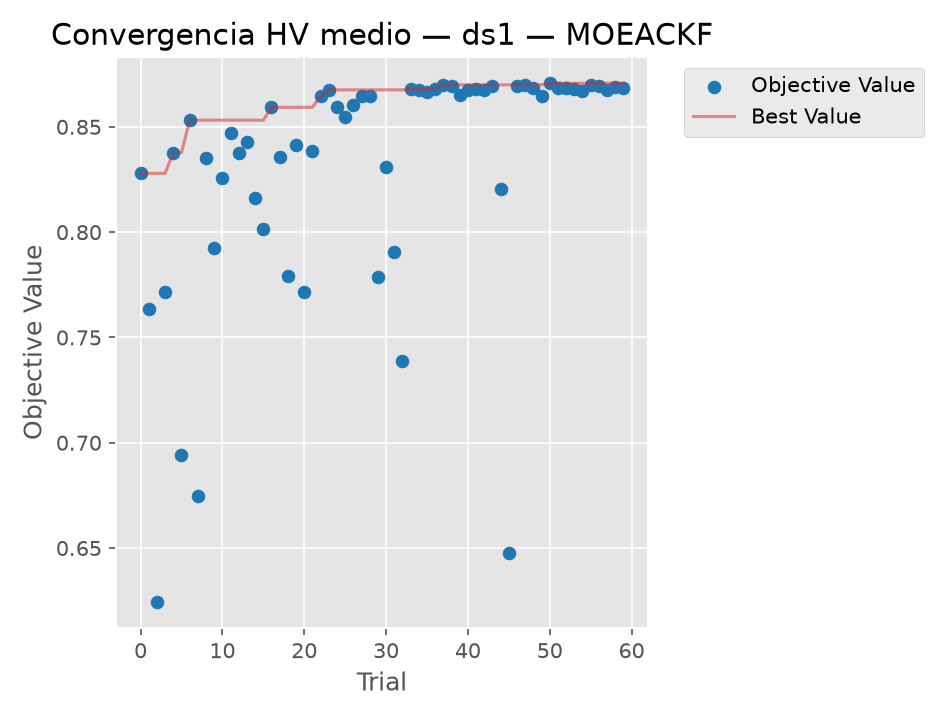
\includegraphics[width=\textwidth]{images/convergencia_MOEACKF_ds1.png}
        \caption{HV medio por trial en \texttt{ds1} para MOEA-CKF.}
        \label{fig:ds1_convergencia_ckf}
    \end{subfigure}
    \hfill
    \begin{subfigure}[b]{0.48\textwidth}
        \centering
        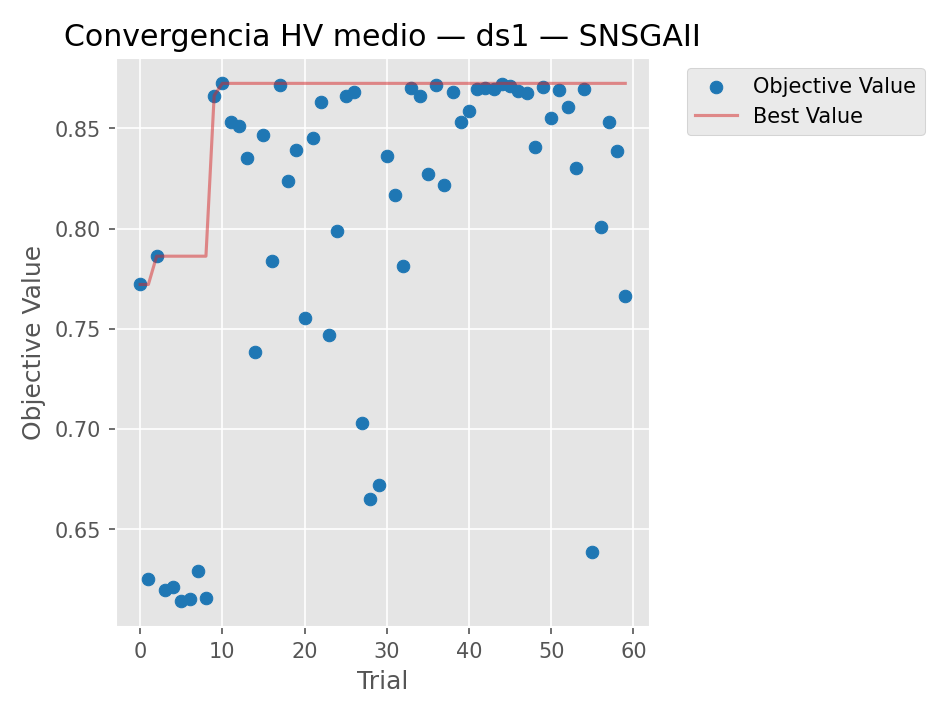
\includegraphics[width=\textwidth]{images/convergencia_SNSGAII_ds1.png}
        \caption{HV medio por \emph{trial} en \texttt{ds1} para S-NSGA-II.}
        \label{fig:ds1_convergencia_nsga}
    \end{subfigure}

    \caption{Convergencia del hipervolumen entre ambos algoritmos para el dataset 1.}
    \label{fig:comparacion_hv_ds1}
\end{figure}

El análisis de importancia de hiperparámetros en \texttt{ds1} muestra que \texttt{wScale} concentra la mayor parte de la varianza explicada del HV en ambos algoritmos, de forma casi absoluta en MOEA-CKF (94.7\%) y más repartida en S-NSGA-II (53.7\%), donde \texttt{sLower} aporta una contribución secundaria relevante (31.8\%). Estas relaciones se muestran en las Figuras~\ref{fig:ds1_fanova_ckf} y~\ref{fig:ds1_fanova_nsga}.

\begin{figure}[htbp]
    \centering
    \begin{subfigure}[b]{0.48\textwidth}
        \centering
        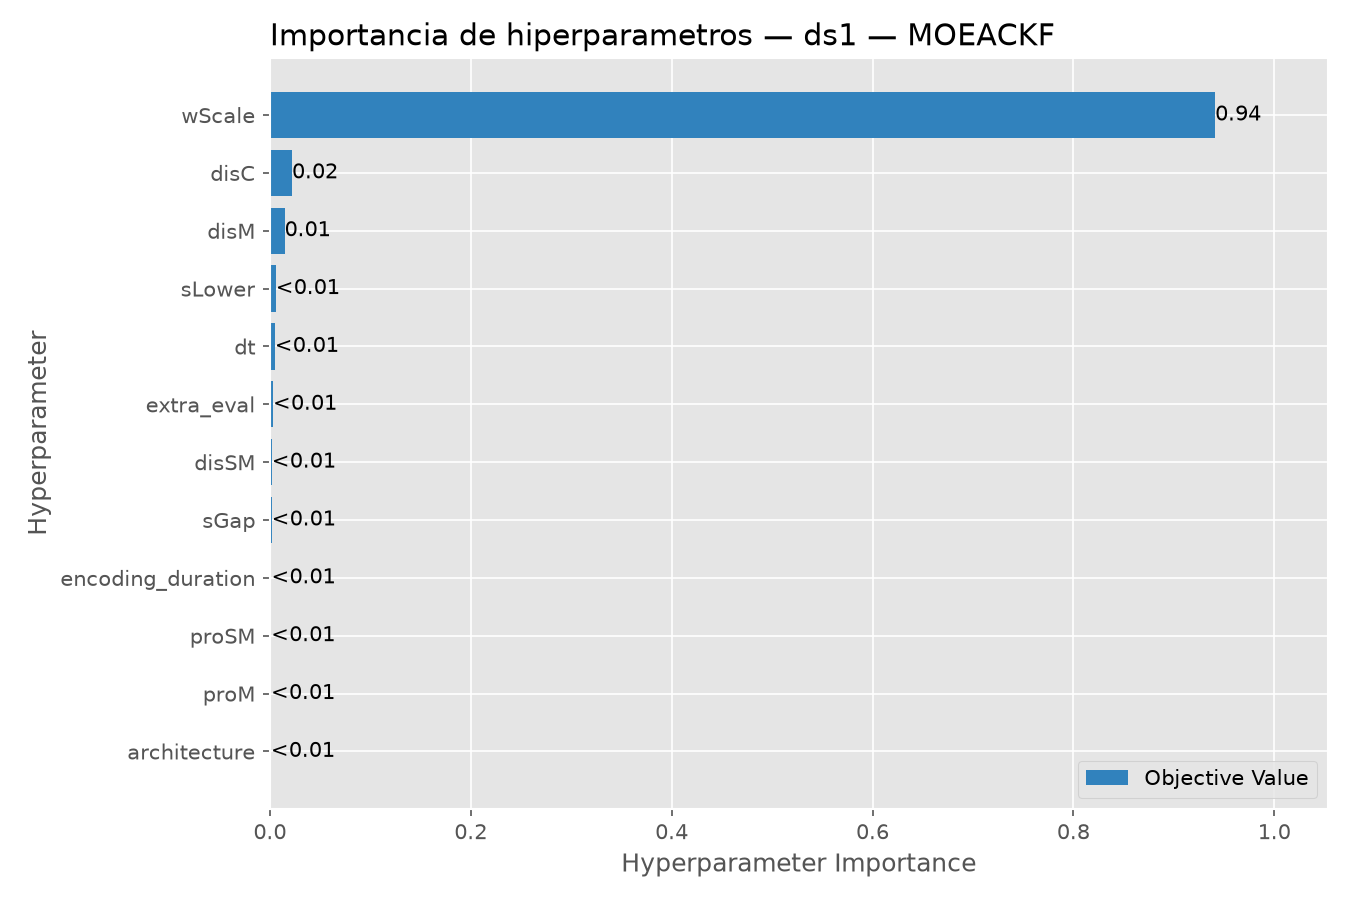
\includegraphics[width=\textwidth]{images/importancia_MOEACKF_ds1.png}
        \caption{Importancia de hiperparámetros (fANOVA) en \texttt{ds1} para MOEA-CKF (corresponde a la Figura~11).}
        \label{fig:ds1_fanova_ckf}
    \end{subfigure}
    \hfill
    \begin{subfigure}[b]{0.48\textwidth}
        \centering
        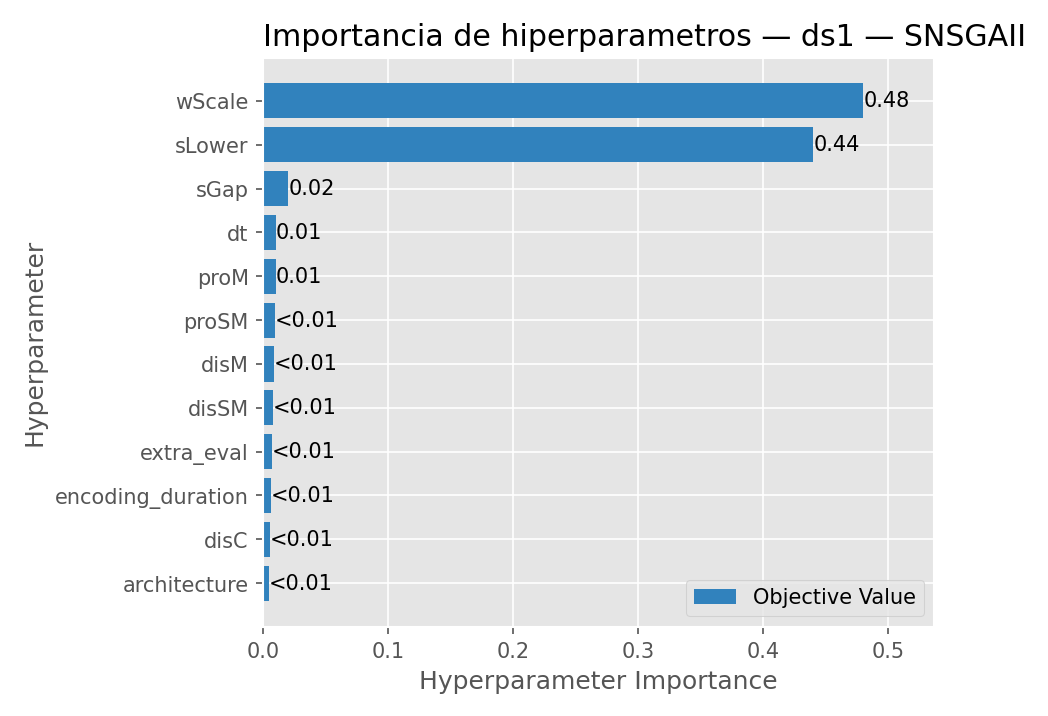
\includegraphics[width=\textwidth]{images/importancia_SNSGAII_ds1.png}
        \caption{Importancia de hiperparámetros (fANOVA) en \texttt{ds1} para S-NSGA-II (corresponde a la Figura~12).}
        \label{fig:ds1_fanova_nsga}
    \end{subfigure}

    \caption{Importancia de hiperparámetros en \texttt{ds1} para ambos algoritmos.}
    \label{fig:importancia_hiper_ds1}
\end{figure}

\subsubsection{Dataset 2: Climate}


Los mejores HV medios alcanzados en \texttt{ds2} son 0.9297 para MOEA-CKF y 0.9291 para S-NSGA-II. La configuración ganadora correspondió a TTFS en MOEA-CKF y Poisson en S-NSGA-II. Las Figuras~\ref{fig:ds2_convergencia_ckf} y~\ref{fig:ds2_convergencia_nsga} muestran la convergencia del HV medio por \emph{trial} para MOEA-CKF y S-NSGA-II en \texttt{ds2}, respectivamente, concentrando los HV en una banda alta y estrecha entre 0.91 y 0.93.

\begin{figure}[htbp]
    \centering
    \begin{subfigure}[b]{0.48\textwidth}
        \centering
        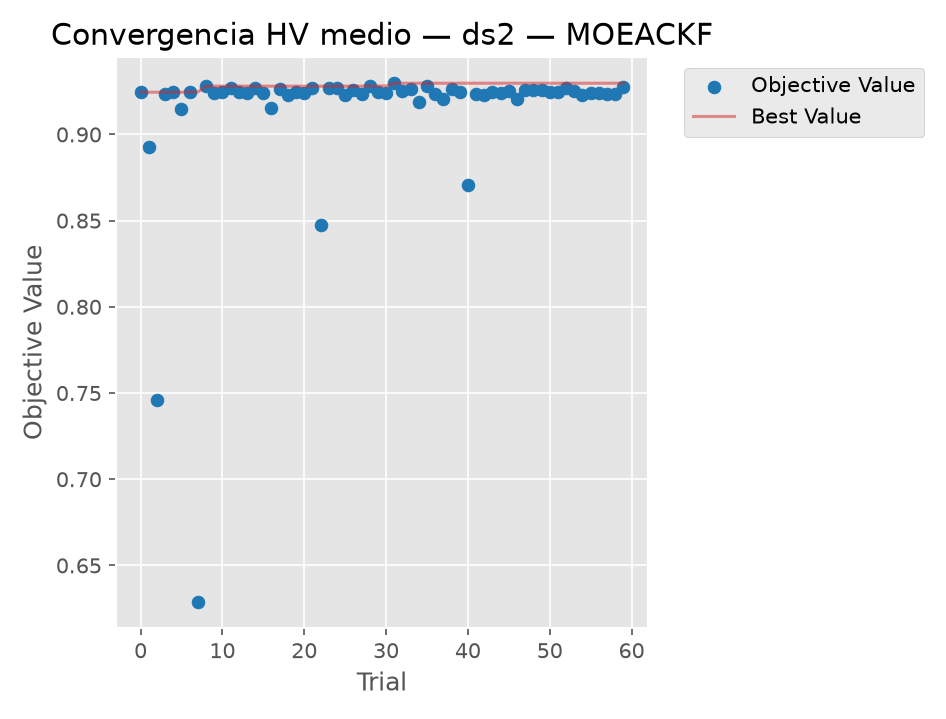
\includegraphics[width=\textwidth]{images/convergencia_MOEACKF_ds2.png}
        \caption{Convergencia del HV medio por \emph{trial} en \texttt{ds2} para MOEA-CKF.}
        \label{fig:ds2_convergencia_ckf}
    \end{subfigure}
    \hfill
    \begin{subfigure}[b]{0.48\textwidth}
        \centering
        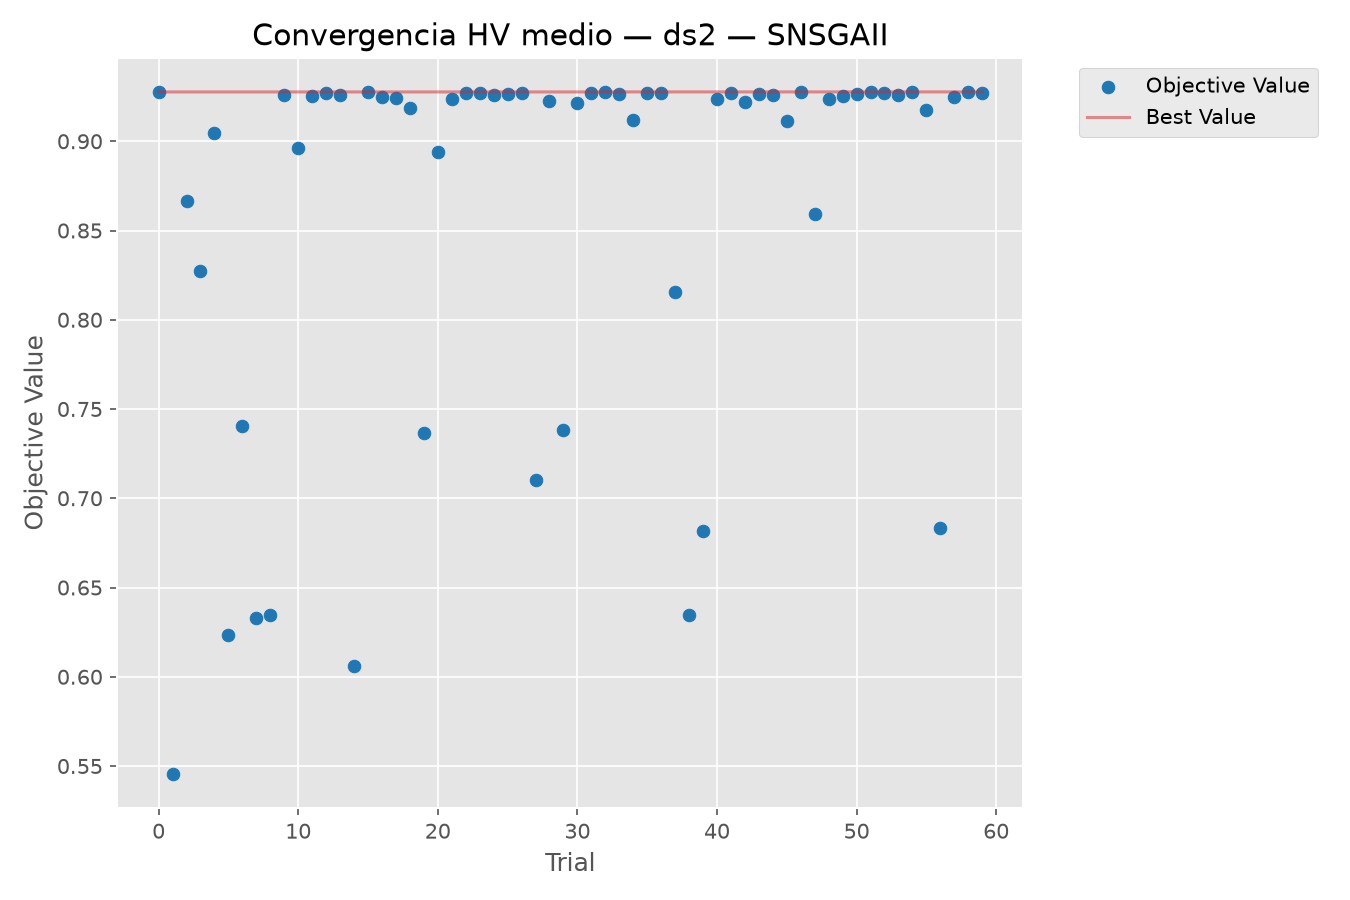
\includegraphics[width=\textwidth]{images/convergencia_SNSGAII_ds2.png}
        \caption{Convergencia del HV medio por \emph{trial} en \texttt{ds2} para S-NSGA-II.}
        \label{fig:ds2_convergencia_nsga}
    \end{subfigure}

    \caption{Comparación de convergencia del hipervolumen entre ambos algoritmos para el Dataset 2.}
    \label{fig:comparacion_hv_ds2}
\end{figure}

El análisis fANOVA en \texttt{ds2} muestra que, al igual que en \texttt{ds1}, es \texttt{wScale} quien concentra casi toda la varianza explicada del HV en ambos algoritmos (95.9\% en MOEA-CKF, 96.2\% en S-NSGA-II), mientras que \texttt{architecture} queda con una importancia prácticamente nula (por debajo del 0.2\% en ambos algoritmos), consistente con que ninguna de las dos resulte claramente superior a la otra en este dataset (Tabla~\ref{tab:hv_por_dataset_resultados}). Esta relación se ilustra en las Figuras~\ref{fig:ds2_fanova_ckf} y~\ref{fig:ds2_fanova_nsga}.

\begin{figure}[htbp]
    \centering

    \begin{subfigure}[b]{0.48\textwidth}
        \centering
        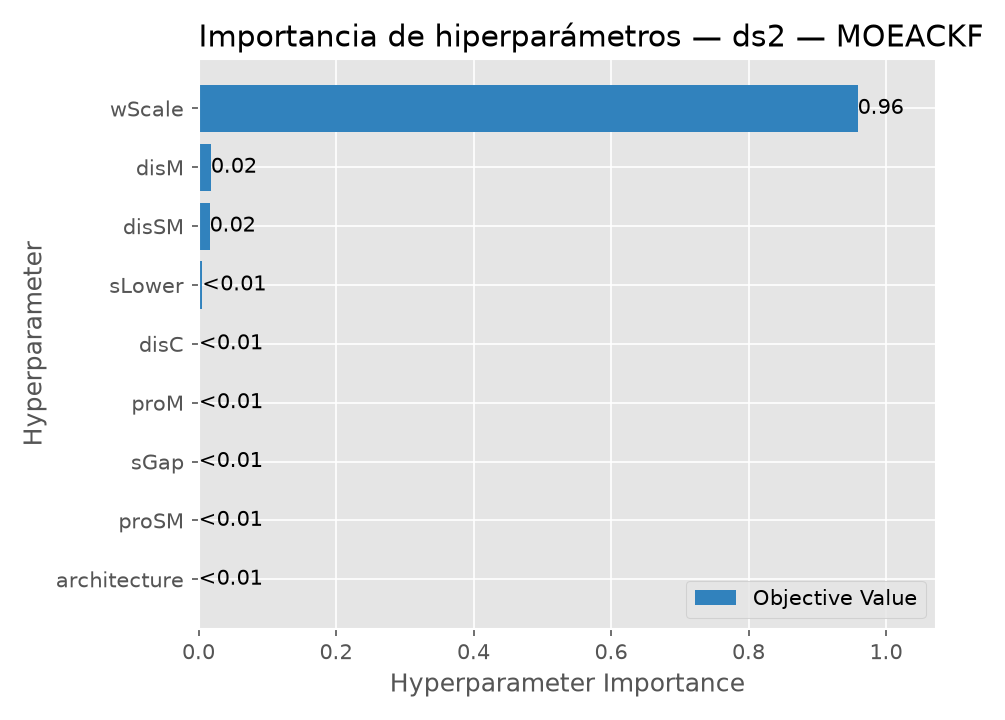
\includegraphics[width=\textwidth]{images/importancia_MOEACKF_ds2.png}
        \caption{Importancia de hiperparámetros (fANOVA) en \texttt{ds2} para MOEA-CKF.}
        \label{fig:ds2_fanova_ckf}
    \end{subfigure}
    \hfill
    \begin{subfigure}[b]{0.48\textwidth}
        \centering
        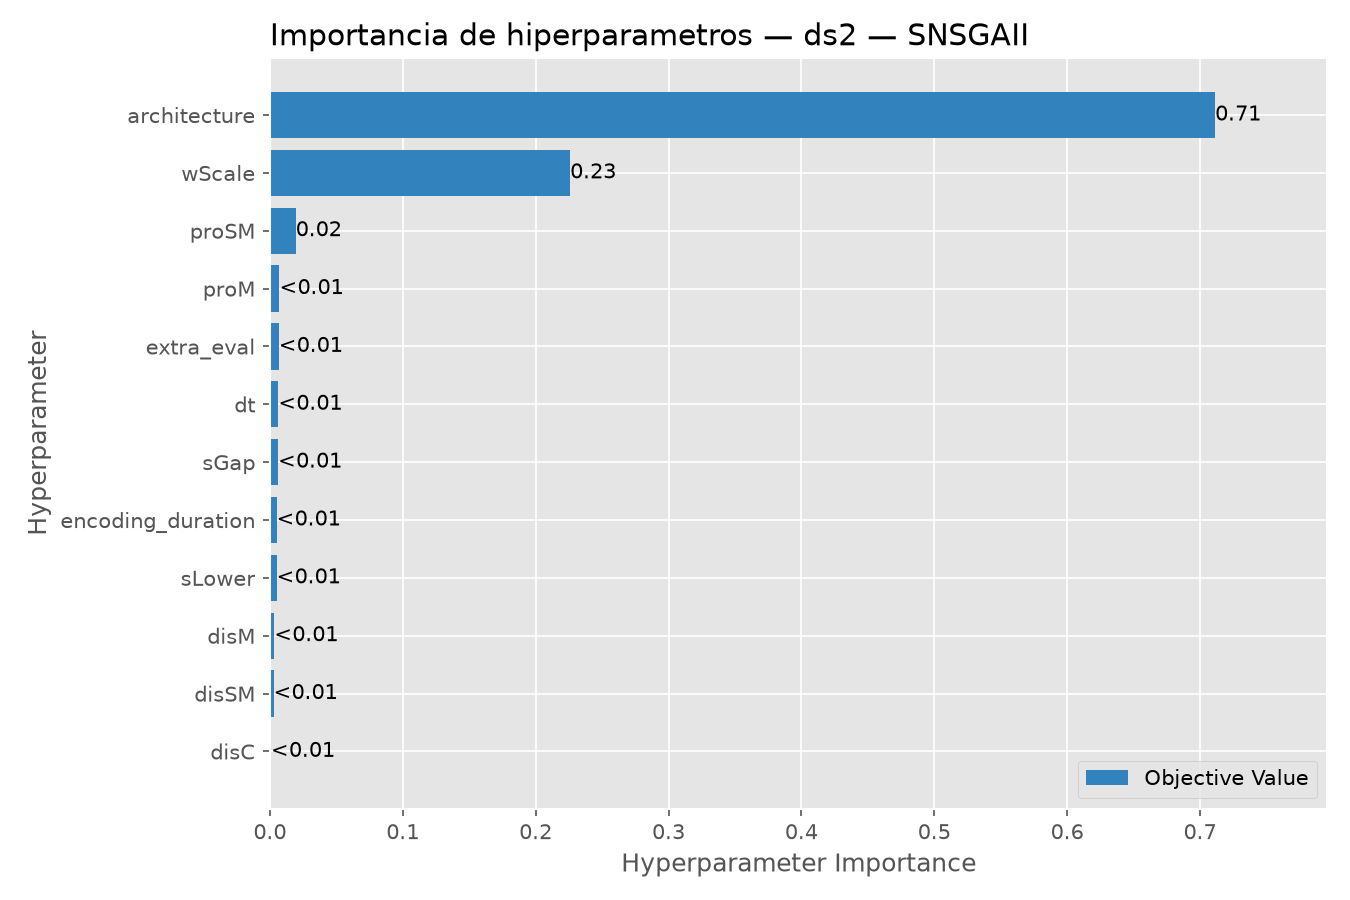
\includegraphics[width=\textwidth]{images/importancia_SNSGAII_ds2.png}
        \caption{Importancia de hiperparámetros (fANOVA) en \texttt{ds2} para S-NSGA-II.}
        \label{fig:ds2_fanova_nsga}
    \end{subfigure}

    \caption{Importancia de hiperparámetros en \texttt{ds2} para ambos algoritmos.}
    \label{fig:importancia_hiper_ds2}
\end{figure}

\subsubsection{Dataset 3: Statlog German}

En este dataset ambos algoritmos alcanzan un HV medio muy cercano, con S-NSGA-II por sobre MOEA-CKF (0.7550 frente a 0.7501). La Tabla~\ref{tab:hiper_mejor_config} muestra que ambas configuraciones difieren en varios hiperparámetros continuos, incluyendo \texttt{wScale} y los límites de esparsidad: MOEA-CKF selecciona una banda de esparsidad orientada a redes muy esparsas (\texttt{sLower} cercana a 0.88), mientras que S-NSGA-II opta por una banda algo más densa (\texttt{sLower}$\approx$0.69).

Las Figuras~\ref{fig:ds3_convergencia_ckf} y~\ref{fig:ds3_convergencia_nsga} ilustran las trayectorias de convergencia del HV medio por \emph{trial} en \texttt{ds3} para ambos algoritmos. Ambos estudios convergen de forma estable hacia el final de los 60 trials, con S-NSGA-II mostrando algo menos de dispersión entre trials cercanos al final de la búsqueda.

\begin{figure}[htbp]
    \centering
    \begin{subfigure}[b]{0.48\textwidth}
        \centering
        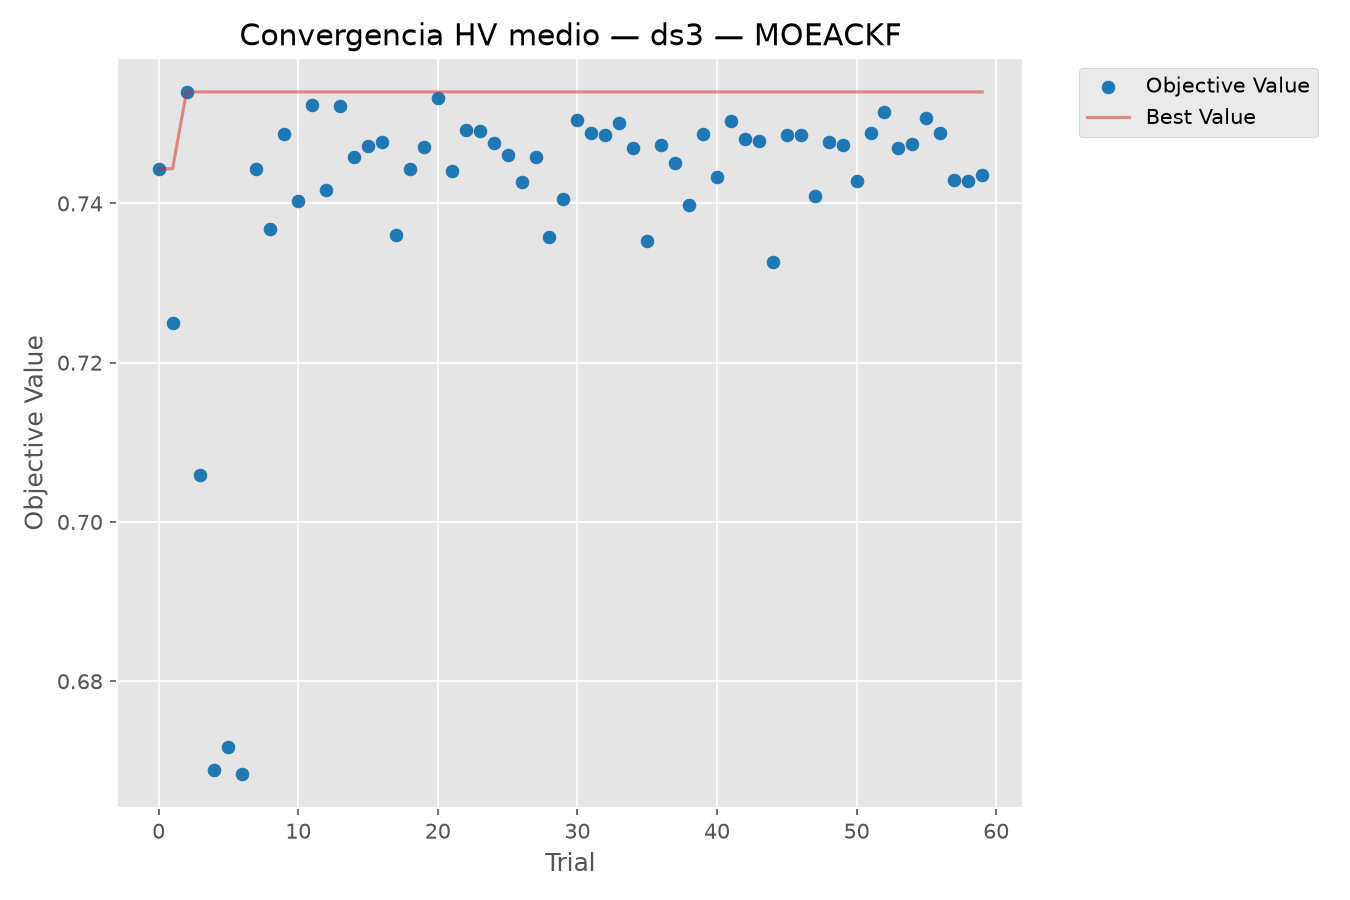
\includegraphics[width=\textwidth]{images/convergencia_MOEACKF_ds3.png}
        \caption{Convergencia del HV medio por \emph{trial} en \texttt{ds3} para MOEA-CKF.}
        \label{fig:ds3_convergencia_ckf}
    \end{subfigure}
    \hfill
    \begin{subfigure}[b]{0.48\textwidth}
        \centering
        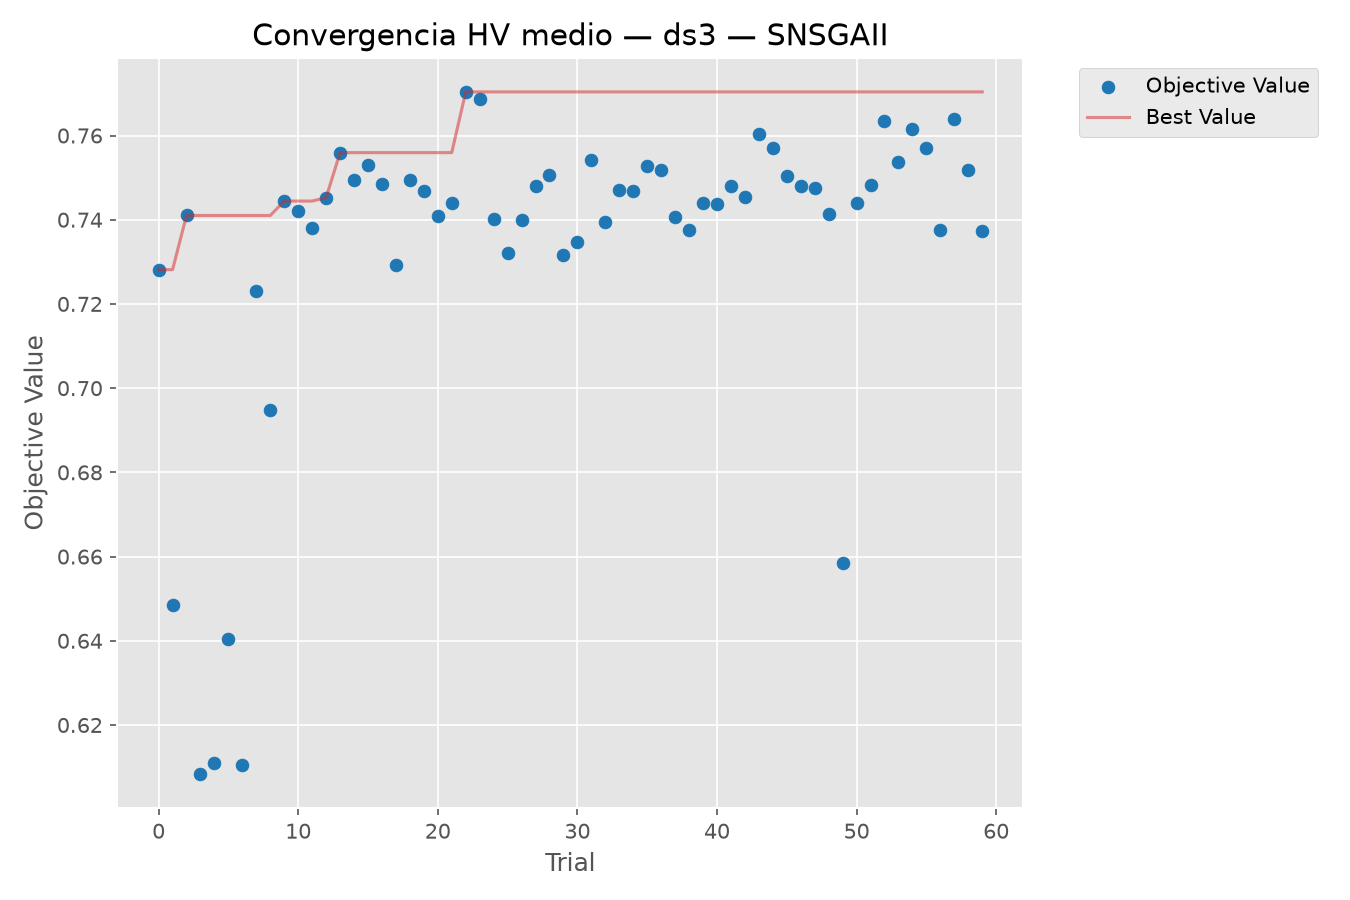
\includegraphics[width=\textwidth]{images/convergencia_SNSGAII_ds3.png}
        \caption{Convergencia del HV medio por \emph{trial} en \texttt{ds3} para S-NSGA-II.}
        \label{fig:ds3_convergencia_nsga}
    \end{subfigure}

    \caption{Comparación de convergencia del hipervolumen entre ambos algoritmos para el Dataset 3.}
    \label{fig:comparacion_hv_ds3}
\end{figure}

En cuanto a la importancia de hiperparámetros, el análisis fANOVA en \texttt{ds3} muestra que \texttt{wScale} vuelve a ser el hiperparámetro más influyente para ambos algoritmos (82.4\% en MOEA-CKF, 89.8\% en S-NSGA-II), con \texttt{proSM} como contribución secundaria en MOEA-CKF (11.4\%). Las Figuras~\ref{fig:ds3_fanova_ckf} y~\ref{fig:ds3_fanova_nsga} reflejan este patrón.

\begin{figure}[htbp]
    \centering

    \begin{subfigure}[b]{0.48\textwidth}
        \centering
        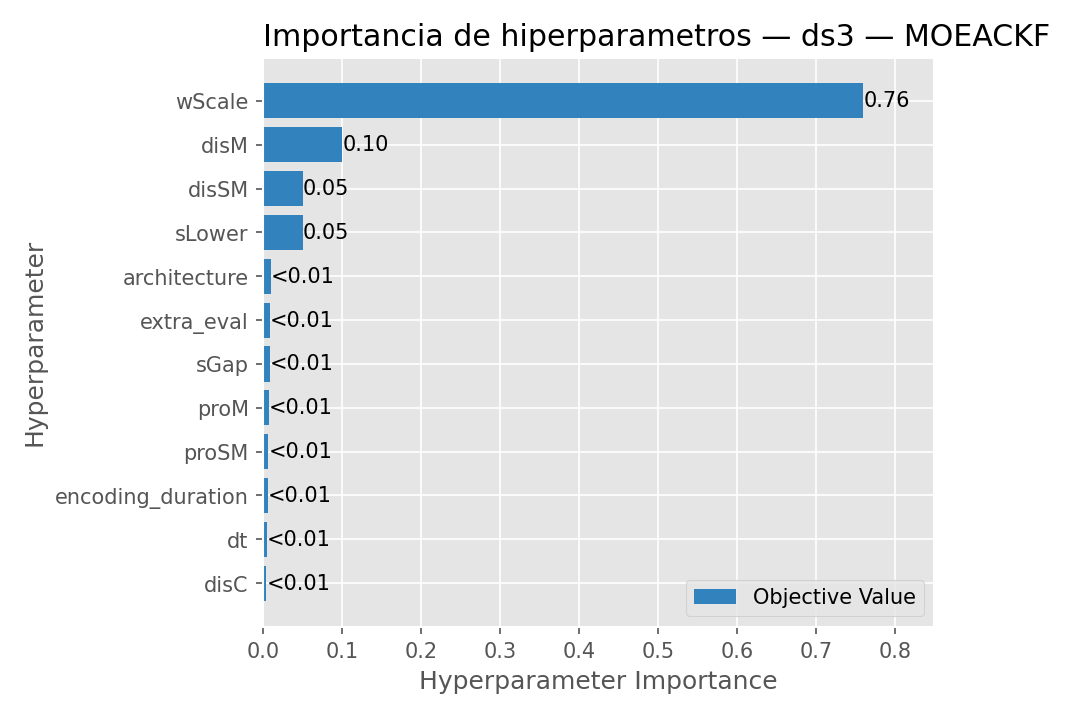
\includegraphics[width=\textwidth]{images/importancia_MOEACKF_ds3.png}
        \caption{Importancia de hiperparámetros (fANOVA) en \texttt{ds3} para MOEA-CKF.}
        \label{fig:ds3_fanova_ckf}
    \end{subfigure}
    \hfill
    \begin{subfigure}[b]{0.48\textwidth}
        \centering
        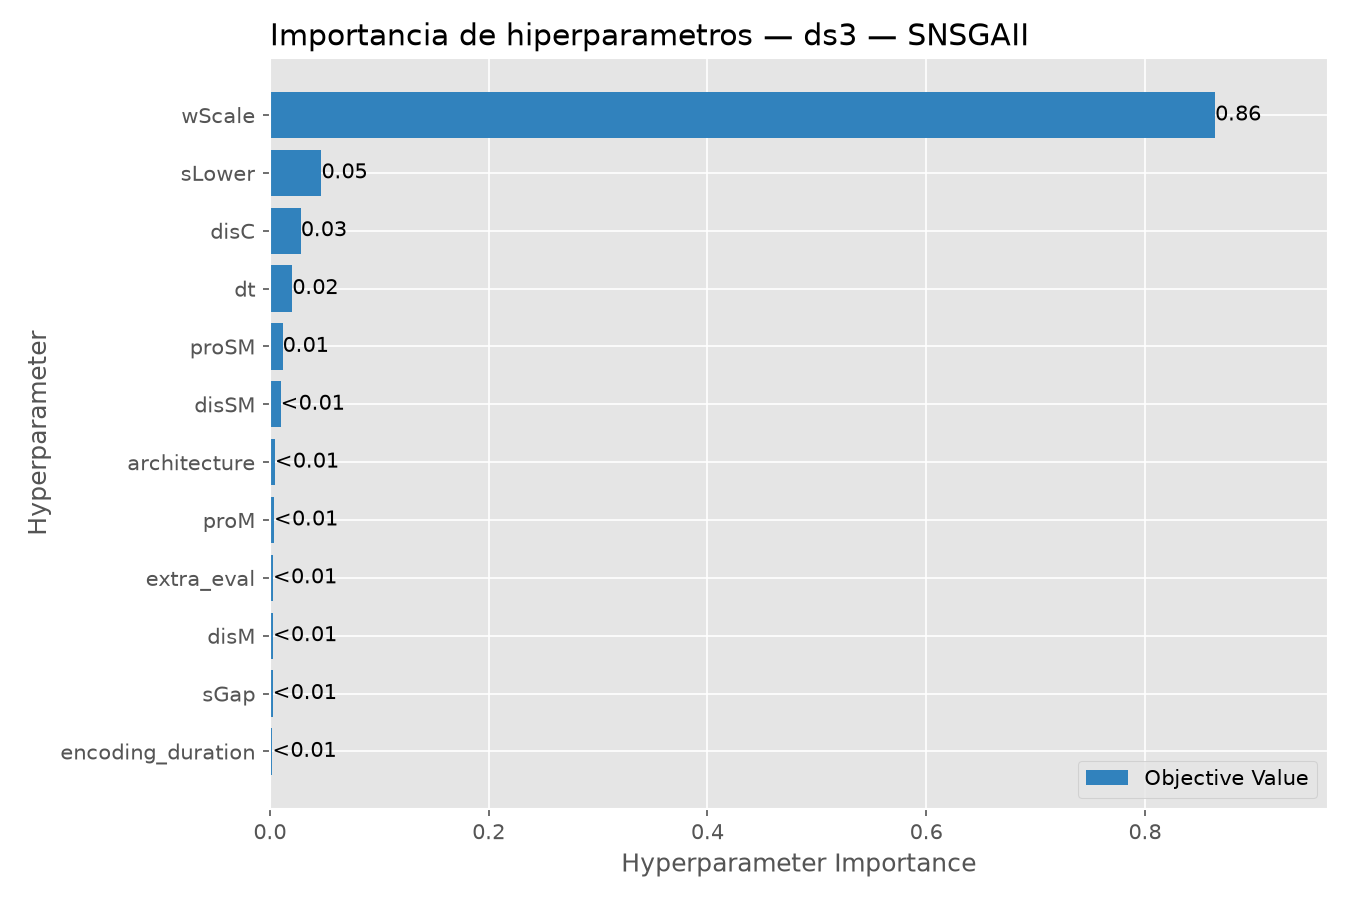
\includegraphics[width=\textwidth]{images/importancia_SNSGAII_ds3.png}
        \caption{Importancia de hiperparámetros (fANOVA) en \texttt{ds3} para S-NSGA-II.}
        \label{fig:ds3_fanova_nsga}
    \end{subfigure}

    \caption{Importancia de hiperparámetros en \texttt{ds3} para ambos algoritmos.}
    \label{fig:importancia_hiper_ds3}
\end{figure}

\subsubsection{Dataset 4: Connectionist Bench Sonar}

En este dataset S-NSGA-II supera a MOEA-CKF por el margen más amplio de los cuatro estudios, con HV medio 0.8268 frente a 0.8008. Las arquitecturas ganadoras tienen codificación TTFS en ambos casos, pero difieren en varios hiperparámetros continuos, incluyendo \texttt{wScale} y los parámetros de esparsidad.

Las Figuras~\ref{fig:ds4_convergencia_ckf} y~\ref{fig:ds4_convergencia_nsga} muestran las curvas de HV medio por \emph{trial} en \texttt{ds4}, evidenciando que tanto MOEA-CKF como S-NSGA-II logran convergencias estables y valores de HV comparables en las últimas iteraciones.

\begin{figure}[htbp]
    \centering
    \begin{subfigure}[b]{0.48\textwidth}
        \centering
        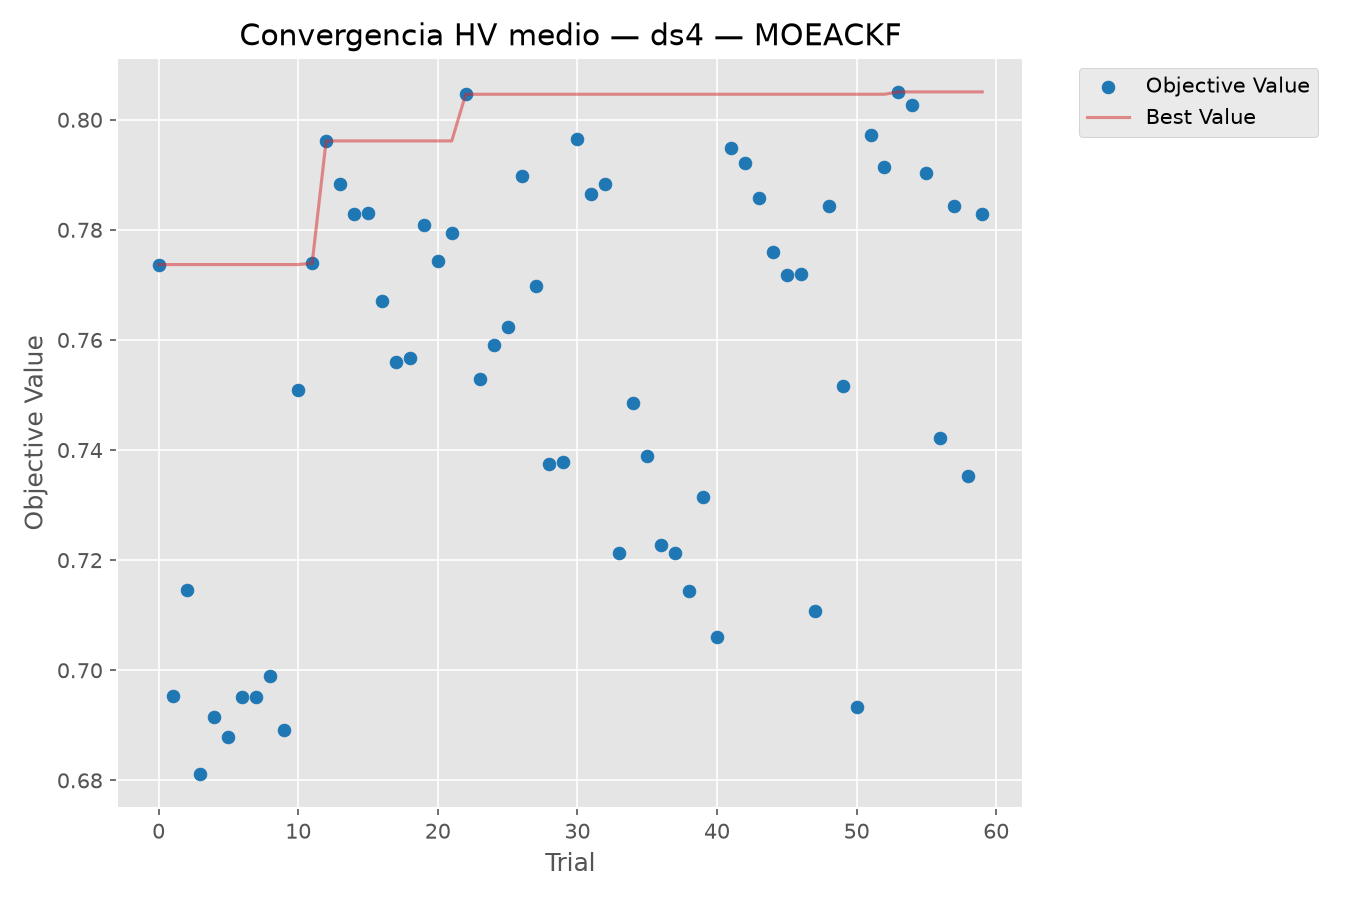
\includegraphics[width=\textwidth]{images/convergencia_MOEACKF_ds4.png}
        \caption{Convergencia del HV medio por \emph{trial} en \texttt{ds4} para MOEA-CKF.}
        \label{fig:ds4_convergencia_ckf}
    \end{subfigure}
    \hfill
    \begin{subfigure}[b]{0.48\textwidth}
        \centering
        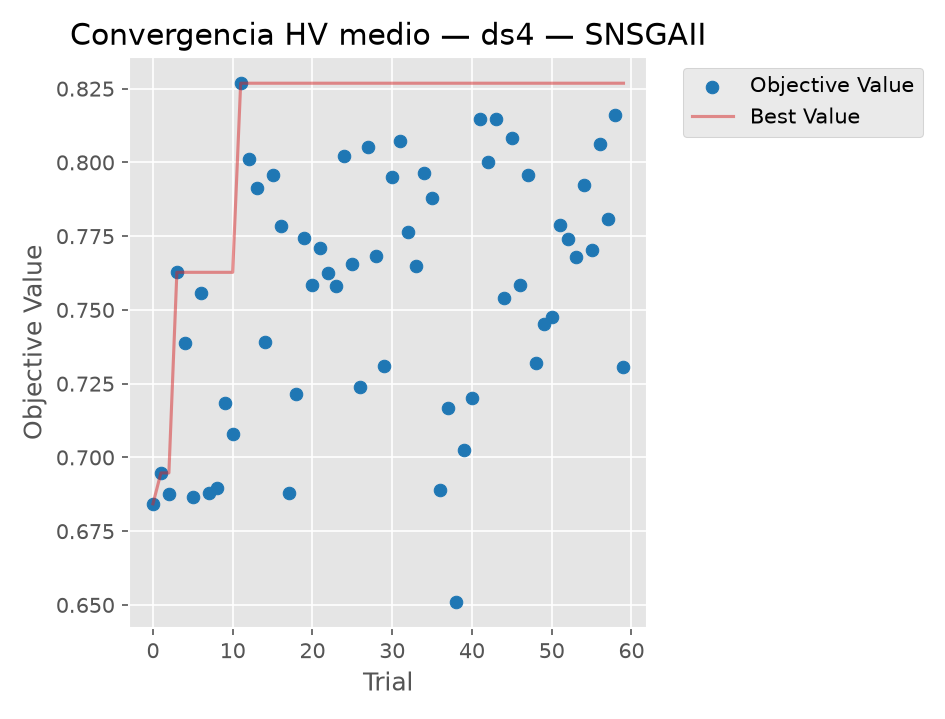
\includegraphics[width=\textwidth]{images/convergencia_SNSGAII_ds4.png}
        \caption{Convergencia del HV medio por \emph{trial} en \texttt{ds4} para S-NSGA-II.}
        \label{fig:ds4_convergencia_nsga}
    \end{subfigure}

    \caption{Comparación de convergencia del hipervolumen entre ambos algoritmos para el Dataset 4.}
    \label{fig:comparacion_hv_ds4}
\end{figure}

El análisis fANOVA en \texttt{ds4} muestra una repartición de importancia más equilibrada y divergente entre algoritmos que en el resto de los datasets: en MOEA-CKF domina \texttt{architecture} (52.7\%), seguido de \texttt{wScale} (32.7\%), mientras que en S-NSGA-II la contribución se reparte principalmente entre \texttt{wScale} (35.9\%) y \texttt{sGap} (35.1\%), con \texttt{sLower} (8.4\%) y \texttt{architecture} (7.9\%) como aportes secundarios. Estos patrones se visualizan en las Figuras~\ref{fig:ds4_fanova_ckf} y~\ref{fig:ds4_fanova_nsga}.

\begin{figure}[htbp]
    \centering

    \begin{subfigure}[b]{0.48\textwidth}
        \centering
        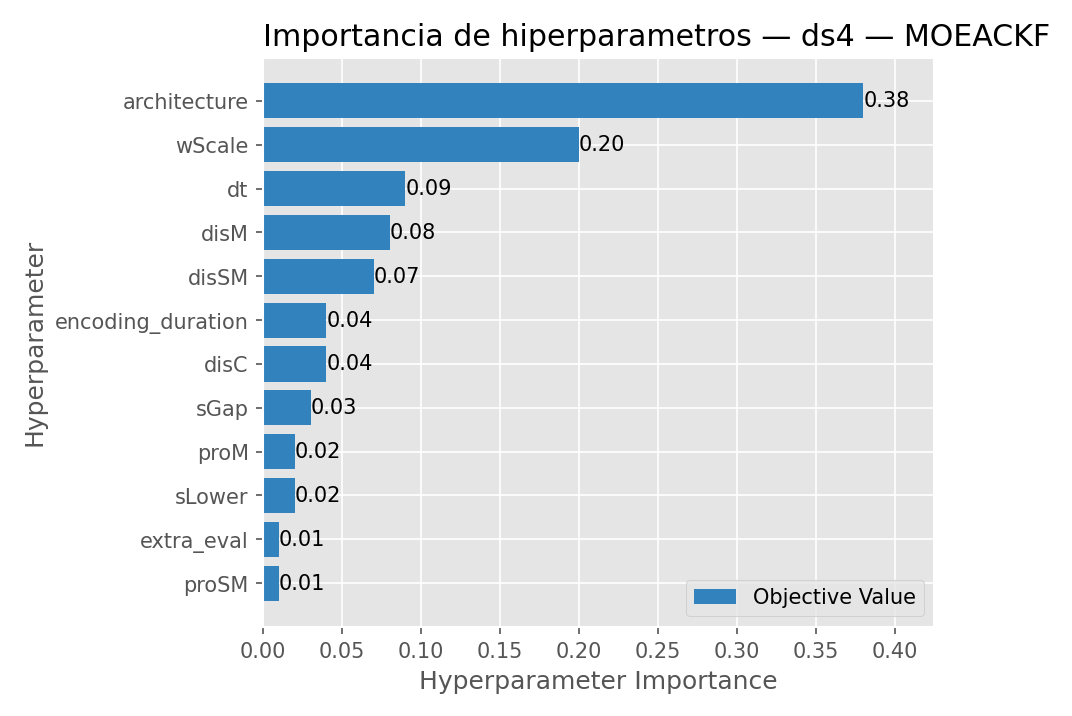
\includegraphics[width=\textwidth]{images/importancia_MOEACKF_ds4.png}
        \caption{Importancia de hiperparámetros (fANOVA) en \texttt{ds4} para MOEA-CKF.}
        \label{fig:ds4_fanova_ckf}
    \end{subfigure}
    \hfill
    \begin{subfigure}[b]{0.48\textwidth}
        \centering
        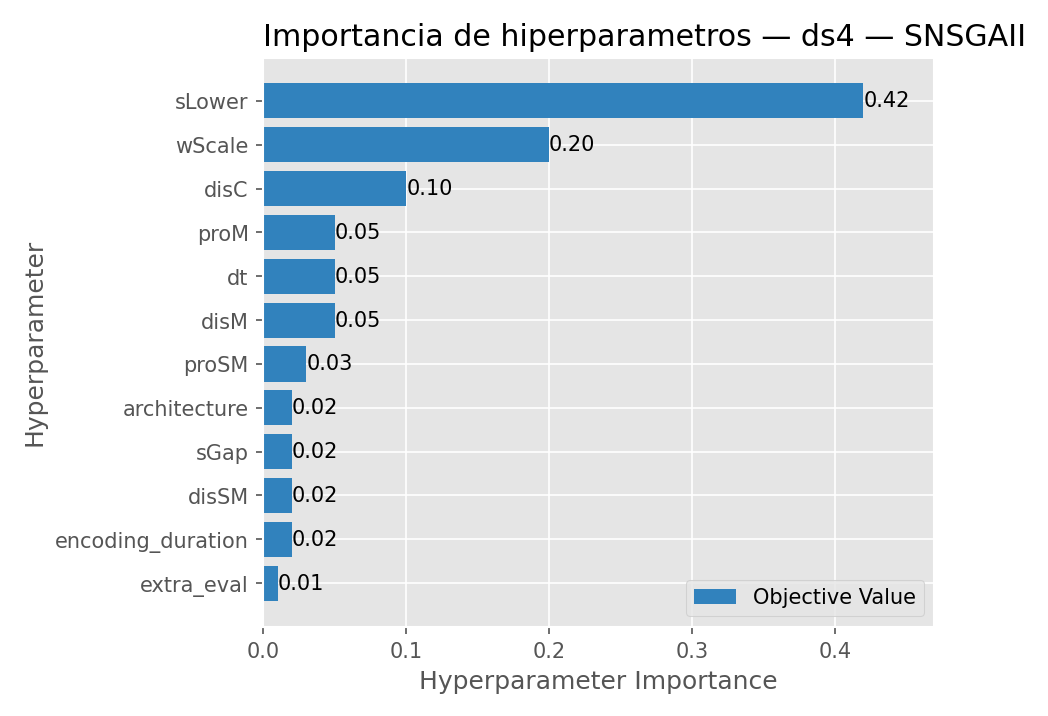
\includegraphics[width=\textwidth]{images/importancia_SNSGAII_ds4.png}
        \caption{Importancia de hiperparámetros (fANOVA) en \texttt{ds4} para S-NSGA-II.}
        \label{fig:ds4_fanova_nsga}
    \end{subfigure}

    \caption{Importancia de hiperparámetros en \texttt{ds4} para ambos algoritmos.}
    \label{fig:importancia_hiper_ds4}
\end{figure}

%-----------------


\providecommand{\Atwelve}{\ensuremath{\hat{A}_{12}}}

\section{Resultados de comparación de algoritmos}
\label{sec:resultados-discusion}

Los resultados y el análisis se organizan en tres experimentos sobre cuatro conjuntos de datos, siguiendo el orden de la Sección~\ref{sec:metodologia-comparacion}. En todos los casos el análisis se realizó por cada dataset, dado que nunca se combinan en una misma prueba estadística. Se reportan los p-valores reportados en cada tabla de los test y su corrección, y se marcaron con \texttt{*} cuando resultaron significativos a $\alpha=0.05$. El veredicto final, obtenido tras aplicar la corrección de Holm-Bonferroni por familias (Sección \ref{subsec:pruebas-estadisticas-correccion}) se menciona en el texto como \textit{tras corrección}. Por último, las tablas reportaron mediana e IQR como estadístico principal, debido a que varios grupos no distribuyen normal, siendo consistente con los tests no paramétricos empleados en todo el documento y la literatura de los algoritmos. Para más detalles sobre los resultados, revisar el repositorio del proyecto en .

\subsection{Comparación de algoritmos en SNN (C++)}
\label{sec:experimento1}

Esta sección compara MOEA-CKF y S-NSGA-II, ambos ejecutados en SNN (C++) sobre el conjunto experimental de referencia ($N=31$ corridas pareadas por semilla), mediante cuatro enfoques: hipervolumen (HV), frentes de Pareto, convergencia y tiempo de cómputo para los cuatro datasets.

\subsubsection{Hipervolumen (HV)}\label{sec:hv}
Los resultados descriptivos se resumen en la Tabla~\ref{tab:hv-summary} para los cuatro datasets. Se muestran la mediana y el IQR. \Atwelve\ se reporta como la fracción de corridas pareadas en las que MOEA-CKF supera a S-NSGA-II (empates cuentan 0.5), de modo que valores por sobre 0.5 favorecen a MOEA-CKF y por debajo de 0.5 favorecen a S-NSGA-II.

\begin{table}[htbp]
\centering
\small
\caption{Resumen del hipervolumen (HV) de MOEA-CKF y S-NSGA-II en los cuatro datasets, $N=31$ corridas pareadas por semilla. El algoritmo con mejor HV estadístico se marca por dataset.}
\label{tab:hv-summary}
\begin{tabular}{cllccc}
\toprule
\textbf{Dataset} & \textbf{MOEA-CKF} & \textbf{S-NSGA-II} & \textbf{$p$ Wilcoxon} & \textbf{$p$ Corregido} & \Atwelve \\
\midrule
1 & \cellcolor{gray!20}$0.8705\ [0.8704,\,0.8721]$ & $0.8459\ [0.7895,\,0.8712]$ & $1.18\times10^{-4}$* & $4.74\times10^{-4}$* & 0.710 \\
2 & \cellcolor{gray!20}$0.9298\ [0.9277,\,0.9319]$ & $0.9278\ [0.9277,\,0.9278]$ & $0.0289$*  & $0.0408$*  & 0.645 \\
3 & $0.7563\ [0.7484,\,0.7634]$ & $0.7520\ [0.7498,\,0.7566]$ & $0.2023$   & $0.2075$   & 0.645 \\
4 & $0.8043\ [0.7936,\,0.8283]$ & \cellcolor{gray!20}$0.8229\ [0.8020,\,0.8418]$ & $0.0051$*  & $0.0254$*  & 0.290 \\
\bottomrule
\end{tabular}
\end{table}

\paragraph{Dataset 1: Statlog Australian}\label{sec:ds1}\label{sec:ds1-hv}
La prueba de Wilcoxon signed-rank arroja una diferencia significativa entre ambos algoritmos, que se mantiene tras la corrección. Esta diferencia se refleja también corrida por corrida: MOEA-CKF superó a S-NSGA-II en 22 de las 31 corridas pareadas (71.0\%), sin empates, lo que corresponde a un efecto a favor de MOEA-CKF.

En este dataset, MOEA-CKF obtiene un HV estadísticamente superior al de S-NSGA-II, con un tamaño de efecto grande. MOEA-CKF es además notablemente más consistente entre corridas: la desviación estándar de S-NSGA-II es cerca de 27 veces la de MOEA-CKF (0.0392 frente a 0.0015), y su corrida más baja queda muy por debajo del mínimo histórico de MOEA-CKF.

\paragraph{Dataset 2: Climate}\label{sec:ds2}\label{sec:ds2-hv}
Existe una diferencia significativa entre ambos algoritmos, que se mantiene tras corrección, aunque de magnitud pequeña: MOEA-CKF superó a S-NSGA-II en 20 de las 31 corridas (64.5\%). La diferencia mediana es de apenas $0.0021$, la más pequeña entre los tres datasets con diferencia significativa, y S-NSGA-II se muestra extremadamente concentrado en torno a su mediana (IQR de solo $0.0001$), mientras que MOEA-CKF exhibe una dispersión bastante mayor (IQR de $0.0042$) pese a tener la mediana más alta.

\paragraph{Dataset 3: Statlog German}\label{sec:ds3}\label{sec:ds3-hv}
No se encuentra una diferencia significativa entre ambos algoritmos, lo que se mantiene tras corrección. MOEA-CKF superó a S-NSGA-II en 20 de las 31 corridas (64.5\%), pero la diferencia mediana es pequeña ($0.0043$) y las medianas de ambos quedan dentro del rango intercuartílico del otro. En conjunto, no hay evidencia suficiente de una diferencia real entre ambos algoritmos en HV para este dataset, pese a que MOEA-CKF gane más seguido corrida por corrida.

\paragraph{Dataset 4: Sonar}\label{sec:ds4}\label{sec:ds4-hv}
Existe una diferencia altamente significativa entre ambos algoritmos, que se mantiene tras corrección. S-NSGA-II superó a MOEA-CKF en 22 de las 31 corridas (71.0\%), lo que corresponde a un efecto a favor de S-NSGA-II.

Este es el único dataset donde se invierte el patrón observado en los tres anteriores: S-NSGA-II supera a MOEA-CKF de forma significativa. Es, además, el dataset con mayor varianza absoluta para ambos algoritmos (60 características), aunque aquí es MOEA-CKF quien muestra la mayor dispersión entre corridas (DE$=0.0326$ frente a $0.0256$ de S-NSGA-II).

\subsubsection{Frentes de Pareto}
\label{sec:fronts}

En la Tabla \ref{tab:fronts-all-datasets} se muestran los resultados de la soluciones de los frentes obtenidos por cada combinación de algoritmo y dataset. La tabla fue construida usando la solución de menor error de entrenamiento por cada una de las 31 corridas.

\begin{table}[htbp]
\centering
\small
\caption{Indicadores de las soluciones de mejor exactitud por corrida para ambos algoritmos en los cuatro datasets en base a la mediana [IQR]. El asterisco (*) indica diferencias estadísticamente significativas, marcando el algoritmo con mejor rendimiento estadístico.}
\label{tab:fronts-all-datasets}

\begin{tabular}{@{}cl|p{3.5cm}p{3.5cm}|cc@{}}
\toprule
\textbf{Dataset} &
\textbf{Indicador} &
\textbf{MOEA-CKF} &
\textbf{S-NSGA-II} &
\textbf{$p$ (Wilcoxon)} &
\Atwelve \\
\midrule

\multirow{3}{*}{1}& Complejidad &
$0.0118\ [0.0088,\,0.0132]$ &
$0.0118\ [0.0074,\,0.0154]$ &
$0.5962$ & 0.581 \\

& Error &
\cellcolor{gray!20}$0.1413\ [0.1395,\,0.1413]$ &
$0.1685\ [0.1395,\,0.2310]$ &
$3.10\times10^{-4}$* & 0.290 \\

& Frente &
$6\ [5,\,7]$ &
$5\ [4,\,7]$ &
$0.4246$ & 0.645 \\
\midrule

\multirow{3}{*}{2}& Complejidad &
$0.0202\ [0.0107,\,0.0339]$ &
\cellcolor{gray!20}$0.0024\ [0.0024,\,0.0048]$ &
$2.86\times10^{-6}$* & 0.919 \\

& Error &
\cellcolor{gray!20}$0.0764\ [0.0741,\,0.0787]$ &
$0.0787\ [0.0787,\,0.0787]$ &
$0.0136$* & 0.306 \\

& Frente &
\cellcolor{gray!20}$5\ [5,\,6]$ &
$3\ [2.5,\,4]$ &
$4.40\times10^{-6}$* & 0.903 \\
\midrule

\multirow{3}{*}{3}& Complejidad &
$0.0120\ [0.0074,\,0.0255]$ &
\cellcolor{gray!20}$0.0028\ [0.0019,\,0.0037]$ &
$3.86\times10^{-6}$* & 0.952 \\

& Error &
$0.2675\ [0.2581,\,0.2762]$ &
$0.2725\ [0.2675,\,0.2750]$ &
$0.1037$ & 0.355 \\

& Frente &
\cellcolor{gray!20}$8\ [5.5,\,10]$ &
$3\ [3,\,4]$ &
$5.26\times10^{-6}$* & 0.935 \\
\midrule

\multirow{3}{*}{4}& Complejidad &
$0.0492\ [0.0167,\,0.0879]$ &
$0.0393\ [0.0333,\,0.0617]$ &
$0.2167$ & 0.548 \\

& Error &
$0.2096\ [0.1856,\,0.2216]$ &
\cellcolor{gray!20}$0.1916\ [0.1707,\,0.2156]$ &
$0.0216$* & 0.677 \\

& Frente &
$10\ [7,\,11.5]$ &
\cellcolor{gray!20}$11\ [9.5,\,14]$ &
$0.0282$* & 0.371 \\

\bottomrule
\end{tabular}
\end{table}

\Atwelve\ se reporta en el mismo sentido que en la Tabla~\ref{tab:hv-summary} (un \Atwelve\ alto significa que MOEA-CKF tiene mayor complejidad o mayor error, no necesariamente que "gane"). En \texttt{ds4}, tanto la diferencia de error como la de tamaño de frente son significativas antes de corrección pero dejan de serlo tras Holm-Bonferroni ($p_{\text{holm}}=0.086$ en ambos casos); se reportan igual en el texto por transparencia, marcando explícitamente que no sobreviven la corrección.

\paragraph{Dataset 1: Statlog Australian}\label{sec:ds1-fronts}
De los tres indicadores, solo la diferencia de error resulta significativa (y se mantiene tras corrección); complejidad y tamaño de frente no muestran diferencias estadísticamente distinguibles entre algoritmos.

El 42.9\% de los puntos del frente combinado de S-NSGA-II están dominados por el de MOEA-CKF, y el 40.0\% en sentido inverso (Figura~\ref{fig:combined-front-ds1}): una cobertura mutua casi simétrica, coherente con que la complejidad y el tamaño de frente no difieran significativamente entre ambos.

\begin{figure}[htbp]
    \centering

    \begin{subfigure}[b]{0.48\textwidth}
        \centering
        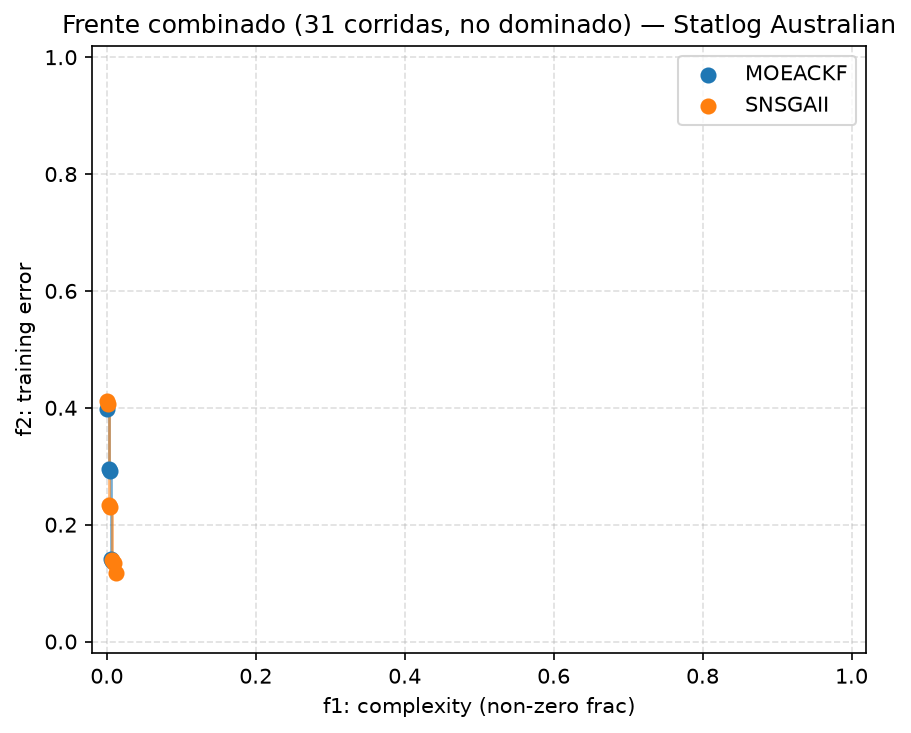
\includegraphics[width=\textwidth]{images/ds1_combined_front.png}
        \caption{Frente combinado (unión no dominada de las 31 corridas) de MOEA-CKF vs.\ S-NSGA-II, dataset 1.}
        \label{fig:combined-front-ds1}
    \end{subfigure}
    \hfill
    \begin{subfigure}[b]{0.48\textwidth}
        \centering
        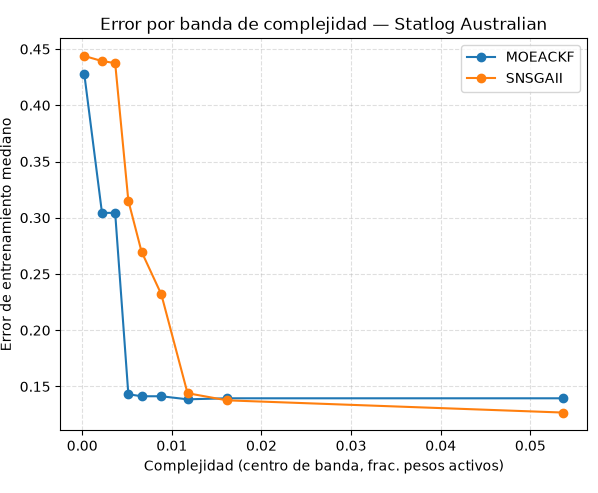
\includegraphics[width=\textwidth]{images/ds1_complexity_bands.png}
        \caption{Error de entrenamiento mediano por banda de complejidad, dataset 1.}
        \label{fig:complexity-bands-ds1}
    \end{subfigure}

    \caption{Frente combinado y bandas de complejidad para dataset 1.}
    \label{fig:frente-bandas-ds1}
\end{figure}

Los deciles sobre el pool de puntos crudos de ambos algoritmos son mostrados en la Figura~\ref{fig:complexity-bands-ds1}. MOEA-CKF obtiene un error mediano menor que S-NSGA-II en la mayoría de las bandas, salvo en una franja de complejidad baja-media ($\sim0.0015$–$0.0044$), donde S-NSGA-II es mejor (p.\,ej.\ $0.251$ vs.\ $0.304$). Ninguno de los dos algoritmos concentra su masa de forma marcadamente distinta de la del otro en este dataset, consistente con la ausencia de diferencia significativa en complejidad y tamaño de frente.

\paragraph{Dataset 2: Climate.}\label{sec:ds2-fronts}
Complejidad y tamaño de frente son significativos y se mantienen tras corrección; el error de las mejores redes también es significativo, aunque con una diferencia mediana pequeña ($0.0764$ vs.\ $0.0787$). En cuanto a complejidad, S-NSGA-II encuentra redes de mejor exactitud más pequeñas que MOEA-CKF con $\Atwelve=0.919$, logrando un error de entrenamiento apenas distinto (y menor) que el de MOEA-CKF. Este último necesita, en cambio, redes más densas y más variables, y retiene además un frente más grande (mediana 5 frente a 3). La cobertura de los frentes combinados no es simétrica: el 33.3\% de los puntos del frente de S-NSGA-II están cubiertos por el de MOEA-CKF, y el 42.9\% en sentido inverso (Figura~\ref{fig:combined-front-ds2}).

\begin{figure}[htbp]
    \centering

    \begin{subfigure}[b]{0.48\textwidth}
        \centering
        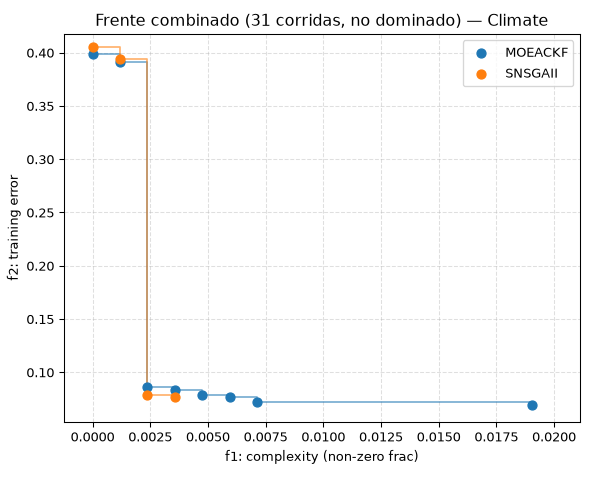
\includegraphics[width=\textwidth]{images/ds2_combined_front.png}
        \caption{Frente combinado (unión no dominada de las 31 corridas) de MOEA-CKF vs.\ S-NSGA-II, dataset 2.}
        \label{fig:combined-front-ds2}
    \end{subfigure}
    \hfill
    \begin{subfigure}[b]{0.48\textwidth}
        \centering
        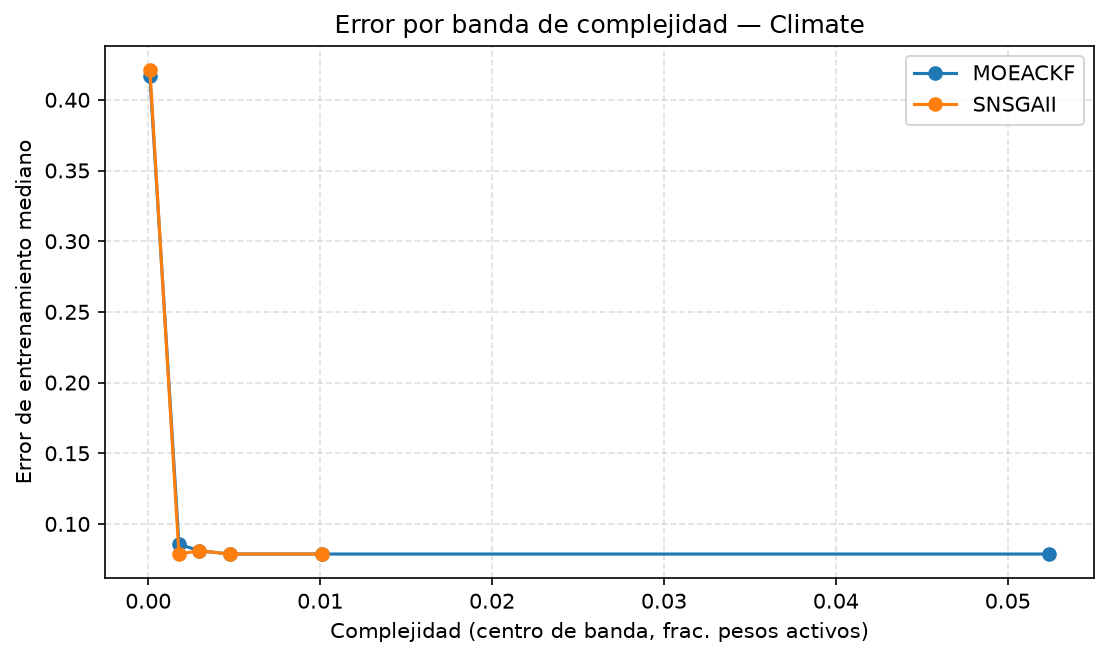
\includegraphics[width=\textwidth]{images/ds2_complexity_bands.png}
        \caption{Error de entrenamiento mediano por banda de complejidad, dataset 2.}
        \label{fig:complexity-bands-ds2}
    \end{subfigure}

    \caption{Frente combinado y bandas de complejidad para dataset 2.}
    \label{fig:frente-bandas-ds2}
\end{figure}

Los deciles sobre el pool de puntos crudos de ambos algoritmos son mostrados en la Figura \ref{fig:complexity-bands-ds2}. S-NSGA-II prácticamente no tiene puntos más allá de la banda de complejidad $0.0060$–$0.0143$ (un solo punto de 31 corridas cae ahí, y ninguno en la banda superior): sus corridas concentran casi toda su masa en las bandas de menor complejidad, mientras que MOEA-CKF se extiende hasta $\sim0.09$. En la banda de complejidad más baja distinta de cero, MOEA-CKF tiene un error mediano algo mayor que S-NSGA-II ($0.0856$ vs.\ $0.0787$); de ahí en adelante ambos convergen al mismo error de $0.0787$, de modo que la ventaja de S-NSGA-II en esta zona es sobre todo de complejidad, no de error.

\paragraph{Dataset 3: Statlog German.}\label{sec:ds3-fronts}
Complejidad y tamaño de frente son significativos y se mantienen tras corrección; la diferencia de error, en cambio, no es significativa. S-NSGA-II incurre en menos complejidad en sus mejores redes, con un error estadísticamente indistinguible del de MOEA-CKF, y retiene frentes sustancialmente más grandes.

Como se observa en la Figura~\ref{fig:combined-front-ds3}, el $20.0\%$ de las soluciones del frente combinado de S-NSGA-II son dominadas por alguna solución de MOEA-CKF. De manera recíproca, MOEA-CKF domina el $50.0\%$ de las soluciones de S-NSGA-II: pese a que MOEA-CKF tiene el doble de puntos en su frente combinado, es su propio frente el más cubierto por el del otro algoritmo, no al revés.

% Este comportamiento sugiere que ninguno de los algoritmos domina de forma concluyente al otro en toda la región de interés. Más bien, ambos conservan soluciones competitivas en distintas zonas del frente de Pareto, aunque S-NSGA-II presenta una mayor capacidad para generar alternativas no dominadas y, con ello, una representación más extensa entre complejidad estructural y error de clasificación.

\begin{figure}[htbp]
    \centering

    \begin{subfigure}[b]{0.48\textwidth}
        \centering
        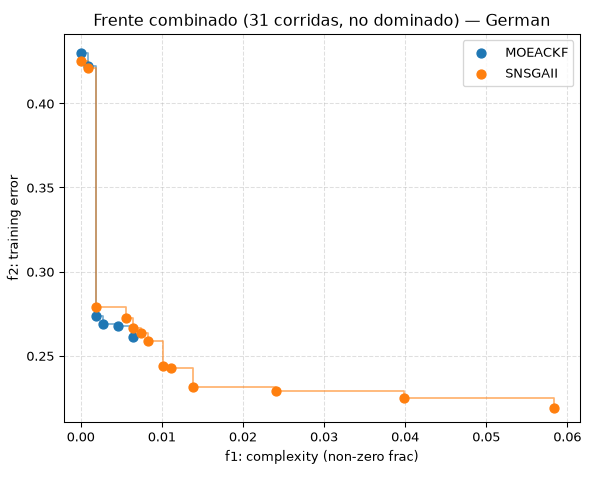
\includegraphics[width=\textwidth]{images/ds3_combined_front.png}
        \caption{Frente combinado (unión no dominada de las 31 corridas) de MOEA-CKF vs.\ S-NSGA-II, dataset 3.}
        \label{fig:combined-front-ds3}
    \end{subfigure}
    \hfill
    \begin{subfigure}[b]{0.48\textwidth}
        \centering
        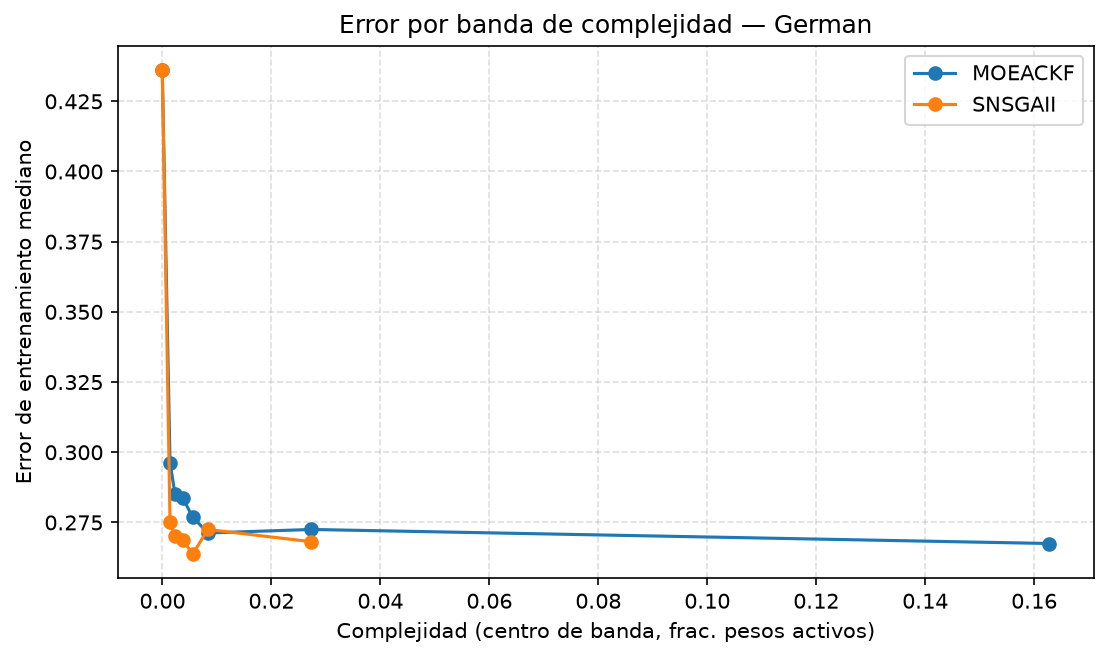
\includegraphics[width=\textwidth]{images/ds3_complexity_bands.png}
        \caption{Error de entrenamiento mediano por banda de complejidad, dataset 3.}
        \label{fig:complexity-bands-ds3}
    \end{subfigure}

    \caption{Frente combinado y bandas de complejidad para dataset 3.}
    \label{fig:frente-bandas-ds3}
\end{figure}

La distribución del error según bandas de complejidad se presenta en la Figura~\ref{fig:complexity-bands-ds3}. En la banda de complejidad nula ambos algoritmos son prácticamente idénticos. Desde $\approx0.001$ y hasta $\approx0.0065$, S-NSGA-II obtiene errores consistentemente menores que MOEA-CKF, aunque con muestras cada vez más pequeñas a medida que sube la complejidad; de ahí en adelante los pocos puntos restantes de S-NSGA-II (2–3 por banda) quedan cerca de MOEA-CKF, y solo este último alcanza la banda de mayor complejidad ($>0.0445$, 37 puntos).

\paragraph{Dataset 4: Sonar}\label{sec:ds4-fronts}

De los tres indicadores, complejidad no resulta significativa; error y tamaño de frente sí lo son antes de corrección, pero ninguno de los dos sobrevive Holm-Bonferroni (ver nota bajo la Tabla~\ref{tab:fronts-all-datasets}). Con esa salvedad, S-NSGA-II tiende a redes con menor error y frentes algo más grandes que MOEA-CKF.

\begin{figure}[htbp]
    \centering

    \begin{subfigure}[b]{0.48\textwidth}
        \centering
        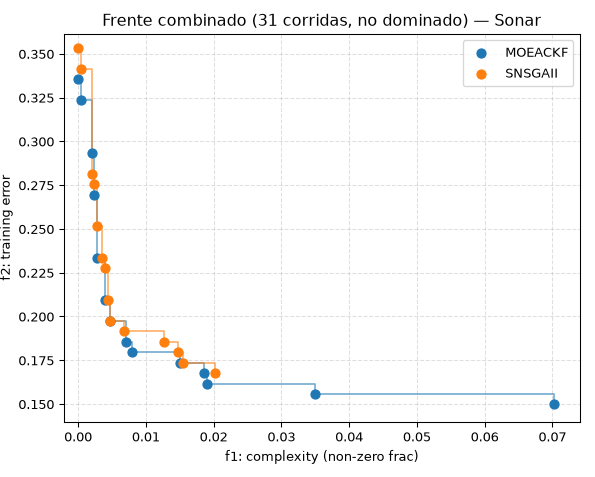
\includegraphics[width=\textwidth]{images/ds4_combined_front.png}
        \caption{Frente combinado (unión no dominada de las 31 corridas) de MOEA-CKF vs.\ S-NSGA-II, dataset 4.}
        \label{fig:combined-front-ds4}
    \end{subfigure}
    \hfill
    \begin{subfigure}[b]{0.48\textwidth}
        \centering
        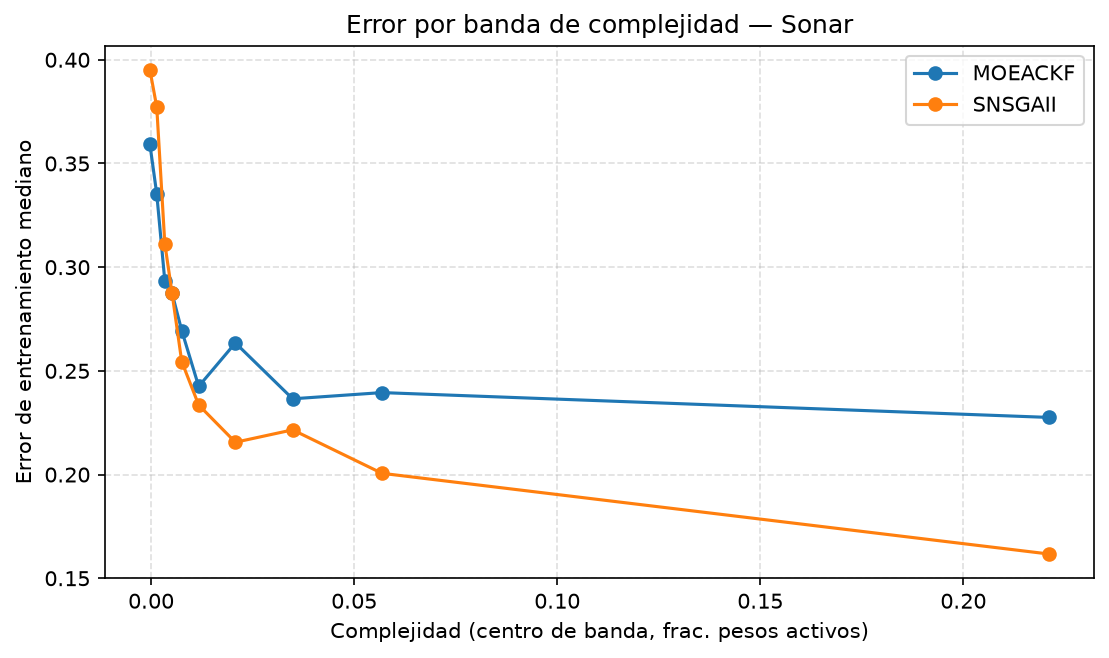
\includegraphics[width=\textwidth]{images/ds4_complexity_bands.png}
        \caption{Error de entrenamiento mediano por banda de complejidad, dataset 4.}
        \label{fig:complexity-bands-ds4}
    \end{subfigure}

    \caption{Frente combinado y bandas de complejidad para dataset 4.}
    \label{fig:frente-bandas-ds4}
\end{figure}

El 84.6\% de las soluciones del frente combinado de MOEA-CKF (13 puntos) son dominadas por alguna solución del frente de S-NSGA-II (14 puntos). Al revés, solo el 21.4\% de las soluciones de S-NSGA-II son dominadas por alguna solución de MOEA-CKF, siendo el resultado más asimétrico de los cuatro datasets, y en sentido opuesto al observado en \texttt{ds3} (Figura~\ref{fig:combined-front-ds4}).

S-NSGA-II presenta un error menor que MOEA-CKF en la mayor parte del rango de complejidad (Figura \ref{fig:complexity-bands-ds4}), con MOEA-CKF por delante únicamente en las tres bandas de menor complejidad (hasta $\approx0.0044$); a partir de ahí S-NSGA-II domina de forma sostenida hasta la banda de mayor complejidad, donde además concentra la muestra más grande de puntos (59 frente a 9 de MOEA-CKF). La ventaja de S-NSGA-II en este dataset es amplia y se concentra en la región de complejidad media a alta, mientras que MOEA-CKF solo es preferible en el extremo más esparso.

\subsubsection{Convergencia}\label{sec:convergencia}

\begin{figure}[htbp]
    \centering

    % Fila 1
    \begin{subfigure}[b]{0.48\textwidth}
        \centering
        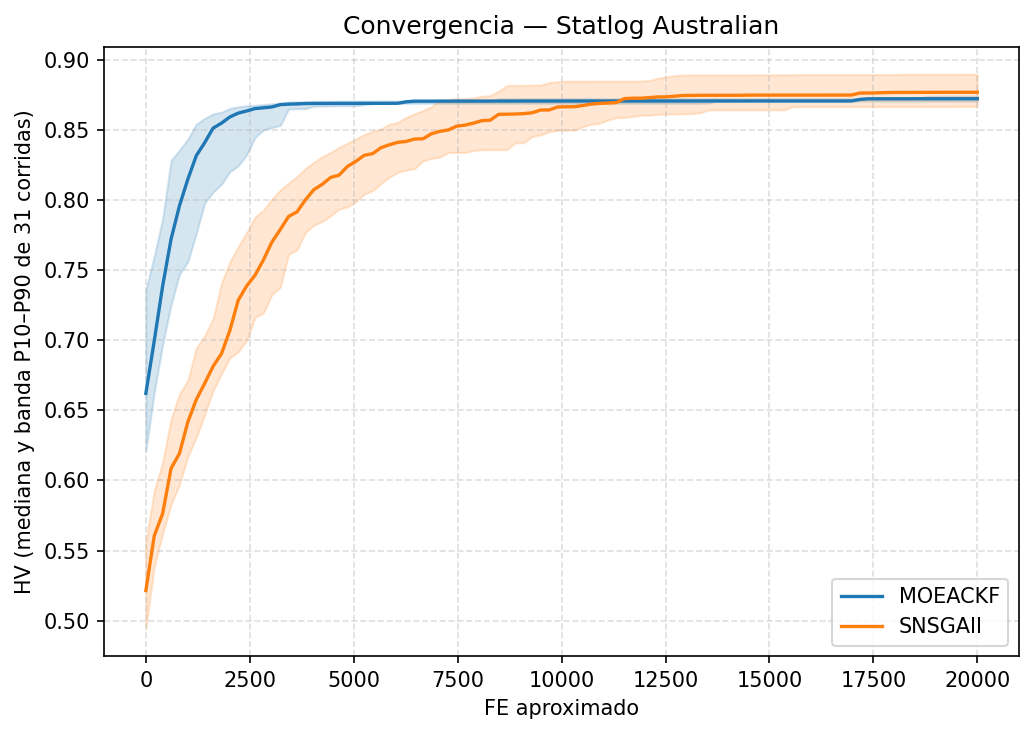
\includegraphics[width=\textwidth]{images/ds1_convergence.png}
        \caption{Curva de convergencia, dataset 1.}
        \label{fig:convergence-ds1}
    \end{subfigure}
    \hfill
    \begin{subfigure}[b]{0.48\textwidth}
        \centering
        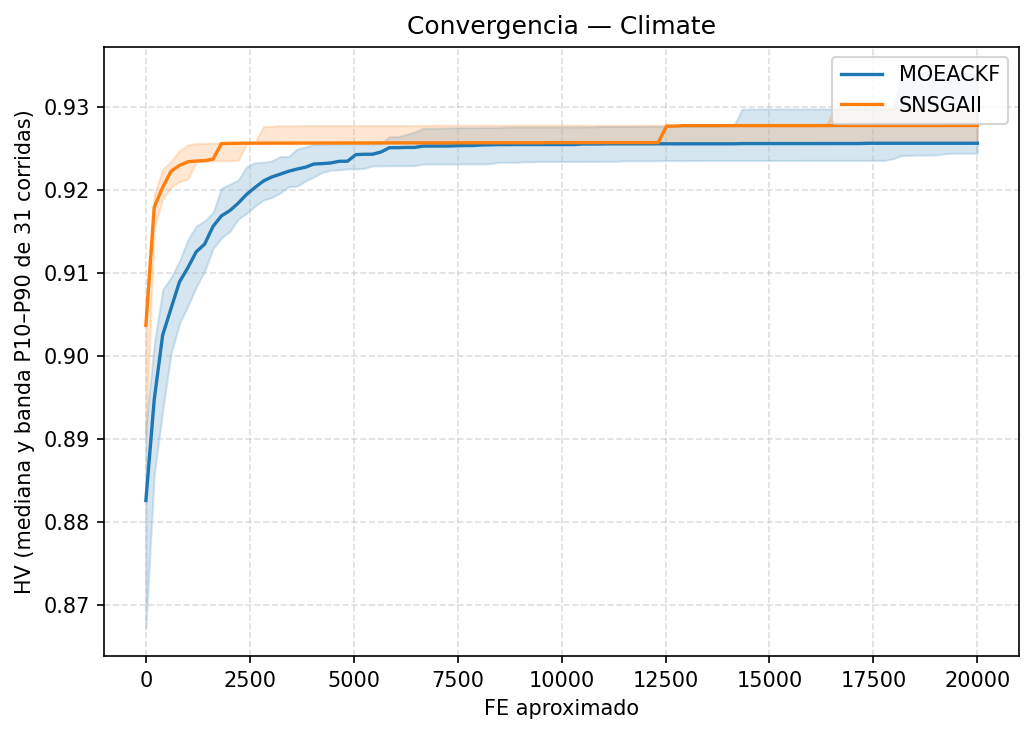
\includegraphics[width=\textwidth]{images/ds2_convergence.png}
        \caption{Curva de convergencia, dataset 2.}
        \label{fig:convergence-ds2}
    \end{subfigure}

    \vspace{0.5cm}

    % Fila 2
    \begin{subfigure}[b]{0.48\textwidth}
        \centering
        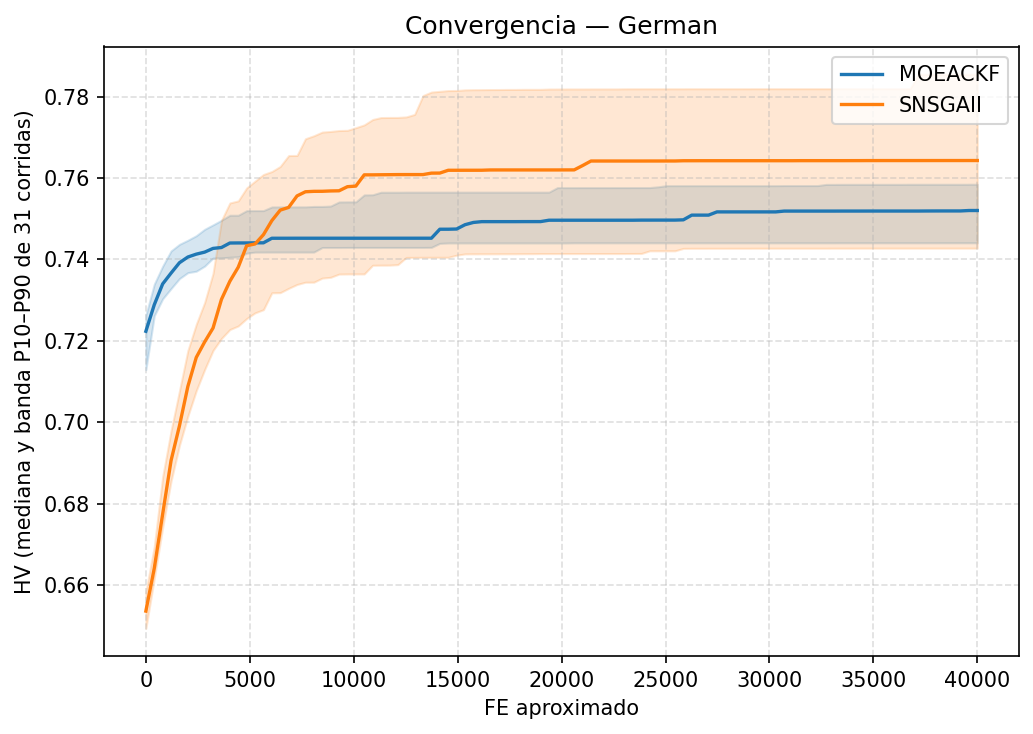
\includegraphics[width=\textwidth]{images/ds3_convergence.png}
        \caption{Curva de convergencia dataset 3.}
        \label{fig:convergence-ds3}
    \end{subfigure}
    \hfill
    \begin{subfigure}[b]{0.48\textwidth}
        \centering
        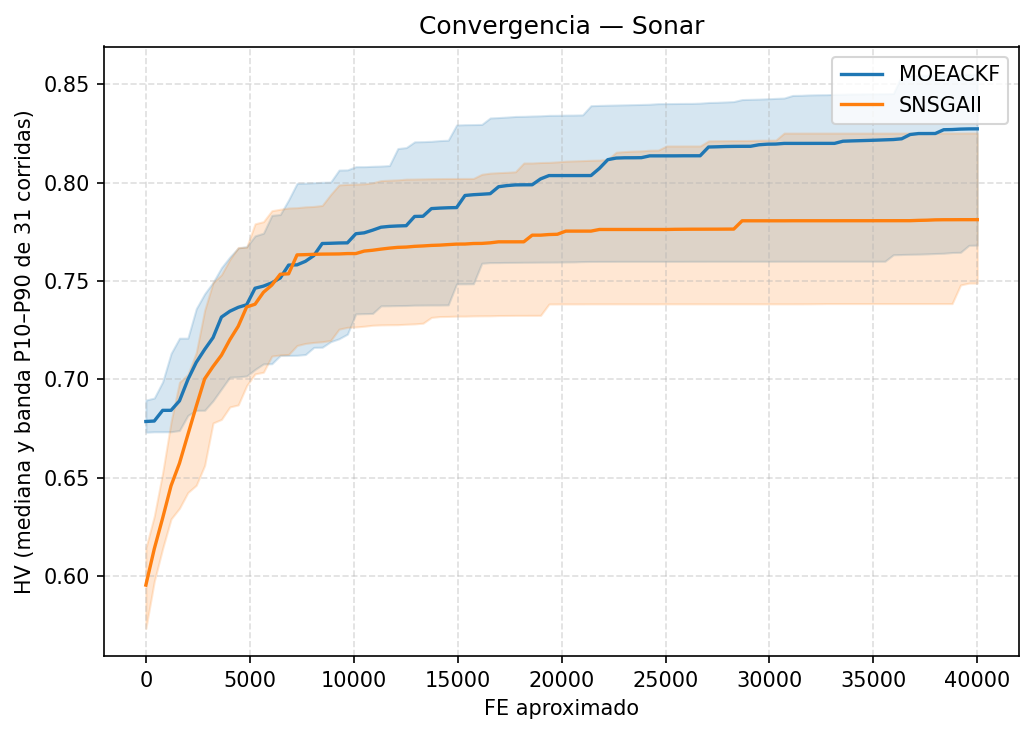
\includegraphics[width=\textwidth]{images/ds4_convergence.png}
        \caption{Curva de convergencia dataset 4.}
        \label{fig:convergence-ds4}
    \end{subfigure}

    \caption{Comparación de las curvas de convergencia para los cuatro datasets.}
    \label{fig:cuadrante}
\end{figure}

\paragraph{Dataset 1: Statlog Australian}\label{sec:ds1-convergencia}

Según la Figura~\ref{fig:convergence-ds1}, MOEA-CKF converge más rápido al comienzo: sube abruptamente y se estabiliza cerca de $\text{FE}\approx3000$-$5000$ en $\text{HV}\approx0.87$. S-NSGA-II, en cambio, arranca más bajo y asciende de forma escalonada, sin llegar a superar el \textit{plateau} de MOEA-CKF y terminando establemente por debajo, en $\text{HV}\approx0.845$.

En las 31 corridas, MOEA-CKF alcanza el 95\% de su propio HV final antes que S-NSGA-II, siendo la diferencia significativa tras corrección. MOEA-CKF en este dataset es más rápido para llegar a su techo como y el que alcanza el techo más alto (Sección~\ref{sec:ds1-hv}).

\paragraph{Dataset 2: Climate}\label{sec:ds2-convergencia}

En las 31 corridas de \textbf{ambos} algoritmos, la población inicial (generación 0) ya alcanza el 90\% del HV final en la mediana, sin diferencia significativa entre algoritmos en ese umbral. Al 95\% sí aparece una diferencia pequeña pero significativa tras corrección: S-NSGA-II llega más consistentemente ya en $\text{FE}\approx0$. 
% (mediana y IQR completos en 0), mientras que el IQR superior de MOEA-CKF llega hasta FE$\approx127$, es decir, unas pocas corridas de MOEA-CKF tardan algo más en estabilizarse. Esto es consistente con que Climate sea, para ambos algoritmos, un problema comparativamente \textit{saturado}: el margen de mejora sobre la población inicial es pequeño, de modo que la velocidad de convergencia aquí mide más bien qué tan rápido se estabiliza la búsqueda que una carrera real de optimización.

\paragraph{Dataset 3: Statlog German}\label{sec:ds3-convergencia}

La curva (Figura~\ref{fig:convergence-ds3}) muestra a S-NSGA-II arrancando más bajo ($\sim0.709$) y ascendiendo con pendiente más pronunciada al inicio, cruzando a MOEA-CKF cerca de $\text{FE}\approx10000$ y manteniéndose por encima de él en la mayor parte del presupuesto restante, aunque con una banda de incertidumbre de MOEA-CKF que se ensancha hacia el final y llega a solaparse con la de S-NSGA-II.

A diferencia de los otros tres datasets, la diferencia de velocidad de convergencia al 95\% no es significativa aquí, aunque la mediana de MOEA-CKF sigue siendo menor que la de S-NSGA-II. Al umbral del 90\% ambos algoritmos alcanzan ese nivel ya en la generación 0 en las 31 corridas, por lo que no hay evidencia de diferencia en ese umbral más laxo.

\paragraph{Dataset 4: Sonar}\label{sec:ds4-convergencia}

Según la Figura~\ref{fig:convergence-ds4}, S-NSGA-II se mantiene por encima de MOEA-CKF durante casi todo el presupuesto y asciende de forma más pronunciada desde el inicio, mientras que MOEA-CKF parte más alto en las primeras evaluaciones pero avanza con mayor lentitud y termina por debajo, sin llegar a aplanarse del todo cerca de $\text{FE}=40000$.

La diferencia de velocidad de convergencia al 95\% no resulta significativa en este dataset, pese a que S-NSGA-II obtiene el HV final más alto (Sección~\ref{sec:ds4-hv}): ambos algoritmos tardan una fracción comparable de su presupuesto en estabilizarse (medianas de $14212$ y $12632$ FE, respectivamente). Al umbral del 90\% sí aparece una diferencia, con MOEA-CKF llegando algo antes.

\subsubsection{Tiempo de cómputo}\label{sec:tiempo-referencia}

Cada algoritmo usa aquí los hiperparámetros que encontró en su propia búsqueda bayesiana, incluyendo el codificador (Poisson o TTFS) y el nivel de esparsidad, por lo que el tiempo medido refleja el costo real incurrido en el experimento principal.

\begin{table}[htbp]
\centering
\small
\caption{Tiempo de ejecución de MOEA-CKF y S-NSGA-II en el conjunto de referencia, $N=31$ corridas pareadas por semilla. Se muestra la mediana [IQR]. El asterisco (*) indica diferencias estadísticamente significativas según la prueba de Wilcoxon. El algoritmo más rápido está destacado.}
\label{tab:time-referencia}
\begin{tabular}{ccccc}
\toprule
\textbf{Dataset} &
\textbf{MOEA-CKF} &
\textbf{S-NSGA-II} &
\textbf{$p$ (Wilcoxon)} &
\Atwelve \\
\midrule

1 &
$275.4\ [259.7,\,284.3]$ s &
\cellcolor{gray!20}$159.5\ [155.3,\,165.3]$ s &
$9.31\times10^{-10}$* & 1.000 \\

2 &
\cellcolor{gray!20}$188.1\ [174.4,\,213.1]$ s &
$223.4\ [204.0,\,243.8]$ s &
$4.53\times10^{-4}$* & 0.226 \\

3 &
\cellcolor{gray!20}$627.8\ [578.8,\,664.6]$ s &
$1026.0\ [995.4,\,1063.0]$ s &
$9.31\times10^{-10}$* & 0.000 \\

4 &
$477.4\ [427.4,\,640.3]$ s &
\cellcolor{gray!20}$167.4\ [166.5,\,170.9]$ s &
$9.31\times10^{-10}$* & 1.000 \\

\bottomrule
\end{tabular}
\end{table}

Las cuatro comparaciones son significativas, tanto antes como después de la corrección por comparaciones múltiples (Tabla~\ref{tab:time-referencia}), y el algoritmo más rápido cambia según el dataset: S-NSGA-II es más rápido en \texttt{ds1} y \texttt{ds4}, mientras que MOEA-CKF lo es en \texttt{ds2} y \texttt{ds3}. Este patrón coincide exactamente con el codificador que cada algoritmo seleccionó en su propia búsqueda de hiperparámetros (Tabla~\ref{tab:hv_por_dataset_resultados}): en \texttt{ds2} y \texttt{ds3}, donde MOEA-CKF gana con TTFS y S-NSGA-II con Poisson, es MOEA-CKF quien resulta más rápido; en \texttt{ds1}, donde los codificadores están invertidos (MOEA-CKF con Poisson, S-NSGA-II con TTFS), es S-NSGA-II quien gana. La única excepción aparente es \texttt{ds4}, donde ambos algoritmos comparten codificador TTFS y, aun así, S-NSGA-II es sustancialmente más rápido (con la mayor brecha relativa de las cuatro, $\Atwelve=1.000$, sin una sola corrida en sentido contrario), lo que aísla un costo algorítmico propio de MOEA-CKF independiente del codificador.

\subsection{Plataforma SNN (C++) vs.\ ANN (MATLAB)}
\label{sec:experimento2}

Esta sección compara cada algoritmo entre su implementación SNN (C++) sobre el conjunto experimental de referencia y la implementación ANN original de PlatEMO/MATLAB, para los cuatro datasets.

\paragraph{Dataset 1: Statlog Australian}
\label{sec:ds1-plataforma}
Las seis comparaciones (Tablas~\ref{tab:platform-MOEA-CKF-ds1} y \ref{tab:platform-S-NSGA-II-ds1}) son significativas y se mantienen tras corrección. La implementación original en ANN (MATLAB) supera de forma consistente a la SNN en HV, con un error de entrenamiento menor para ambos algoritmos y una brecha de error de $\sim0.02$ en MOEA-CKF y $\sim0.06$ en S-NSGA-II. Las redes de menor error en ANN también son más densas que las SNN en ambos algoritmos, con la brecha de complejidad más marcada en S-NSGA-II (impulsada por algunas corridas en MATLAB que alcanzan redes casi densas).

\begin{table}[htbp]
\centering
\small
\caption{MOEA-CKF: SNN vs.\ ANN (MATLAB), dataset 1.}
\label{tab:platform-MOEA-CKF-ds1}
\begin{tabular}{@{}l|p{3.2cm}p{3.2cm}|cc@{}}
\toprule
\textbf{Indicador} & \textbf{MOEA-CKF: SNN} & \textbf{MOEA-CKF: ANN} &
  \textbf{$p$ (Mann-Whitney)} & \Atwelve \\
\midrule
HV &  $0.8705\ [0.8704,\,0.8721]$ &  \cellcolor{gray!20}$0.8891\ [0.8891,\,0.8907]$ &
  $1.37\times10^{-11}$* & 0.000 \\
Complejidad &  \cellcolor{gray!20}$0.0118\ [0.0088,\,0.0132]$ &  $0.0203\ [0.0140,\,0.0390]$ &
  $1.99\times10^{-6}$* & 0.149 \\
Error &  $0.1413\ [0.1395,\,0.1413]$ &  \cellcolor{gray!20}$0.1196\ [0.1178,\,0.1196]$ &
  $5.26\times10^{-12}$* & 1.000 \\
\bottomrule
\end{tabular}

\bigskip
\centering
\caption{S-NSGA-II: SNN vs.\ ANN (MATLAB), dataset 1.}
\label{tab:platform-S-NSGA-II-ds1}
\begin{tabular}{@{}l|p{3.2cm}p{3.2cm}|cc@{}}
\toprule
\textbf{Indicador} & \textbf{S-NSGA-II: SNN} & \textbf{S-NSGA-II: ANN} &
  \textbf{$p$ (Mann-Whitney)} & \Atwelve \\
\midrule
HV &  $0.8459\ [0.7895,\,0.8712]$ &  \cellcolor{gray!20}$0.8972\ [0.8948,\,0.8979]$ &
  $1.54\times10^{-11}$* & 0.001 \\
Complejidad &  \cellcolor{gray!20}$0.0118\ [0.0074,\,0.0154]$ &  $0.0265\ [0.0265,\,0.1256]$ &
  $4.88\times10^{-11}$* & 0.020 \\
Error &  $0.1685\ [0.1395,\,0.2310]$ &  \cellcolor{gray!20}$0.1105\ [0.1096,\,0.1123]$ &
  $1.08\times10^{-11}$* & 1.000 \\
\bottomrule
\end{tabular}
\end{table}

\paragraph{Dataset 2: Climate}
\label{sec:ds2-plataforma}
Todas las comparaciones son significativas tras corrección (Tablas~\ref{tab:platform-MOEA-CKF-ds2} y \ref{tab:platform-S-NSGA-II-ds2}). La brecha ANN-SNN en HV es la más grande de los cuatro datasets para ambos algoritmos, y también lo es en error de entrenamiento. La complejidad, en cambio, diverge fuertemente según el algoritmo: para MOEA-CKF las redes ANN son más densas que las de SNN, mientras que para S-NSGA-II las redes ANN de menor error son casi completamente densas frente a las redes SNN. Para llegar a su menor error, S-NSGA-II-ANN necesita casi todos los pesos activos, mientras que en SNN logra un error de entrenamiento bastante mayor con una fracción minúscula de la red.

\begin{table}[htbp]
\centering
\small
\caption{MOEA-CKF: SNN vs.\ ANN (MATLAB), dataset 2.}
\label{tab:platform-MOEA-CKF-ds2}
\begin{tabular}{@{}l|p{3.2cm}p{3.2cm}|cc@{}}
\toprule
\textbf{Indicador} & \textbf{MOEA-CKF: SNN} & \textbf{MOEA-CKF: ANN} &
  \textbf{$p$ (Mann-Whitney)} & \Atwelve \\
\midrule
HV &  $0.9298\ [0.9277,\,0.9319]$ &  \cellcolor{gray!20}$0.9767\ [0.9747,\,0.9770]$ &
  $1.40\times10^{-11}$* & 0.000 \\
Complejidad &  \cellcolor{gray!20}$0.0202\ [0.0107,\,0.0339]$ &  $0.0487\ [0.0399,\,0.0662]$ &
  $1.88\times10^{-7}$* & 0.114 \\
Error &  $0.0764\ [0.0741,\,0.0787]$ &  \cellcolor{gray!20}$0.0232\ [0.0232,\,0.0255]$ &
  $7.31\times10^{-12}$* & 1.000 \\
\bottomrule
\end{tabular}

\bigskip
\centering
\caption{S-NSGA-II: SNN vs.\ ANN (MATLAB), dataset 2.}
\label{tab:platform-S-NSGA-II-ds2}
\begin{tabular}{@{}l|p{3.2cm}p{3.2cm}|cc@{}}
\toprule
\textbf{Indicador} & \textbf{S-NSGA-II: SNN} & \textbf{S-NSGA-II: ANN} &
  \textbf{$p$ (Mann-Whitney)} & \Atwelve \\
\midrule
HV &  $0.9278\ [0.9277,\,0.9278]$ &  \cellcolor{gray!20}$0.9477\ [0.9440,\,0.9539]$ &
  $1.39\times10^{-11}$* & 0.000 \\
Complejidad &  \cellcolor{gray!20}$0.0024\ [0.0024,\,0.0048]$ &  $0.9114\ [0.7316,\,0.9601]$ &
  $5.12\times10^{-12}$* & 0.000 \\
Error &  $0.0787\ [0.0787,\,0.0787]$ &  \cellcolor{gray!20}$0.0347\ [0.0301,\,0.0370]$ &
  $3.04\times10^{-12}$* & 1.000 \\
\bottomrule
\end{tabular}
\end{table}

\paragraph{Dataset 3: Statlog German}
\label{sec:ds3-plataforma}
Todas las comparaciones son significativas tras corrección (Tablas~\ref{tab:platform-MOEA-CKF-ds3} y \ref{tab:platform-S-NSGA-II-ds3}): las redes ANN de MOEA-CKF son más densas que las SNN, mientras que las redes ANN de S-NSGA-II vuelven a ser casi totalmente densas frente a redes SNN mucho más esparsas.

\begin{table}[htbp]
\centering
\small
\caption{MOEA-CKF: SNN vs.\ ANN (MATLAB), dataset 3.}
\label{tab:platform-MOEA-CKF-ds3}
\begin{tabular}{@{}l|p{3.2cm}p{3.2cm}|cc@{}}
\toprule
\textbf{Indicador} & \textbf{MOEA-CKF: SNN} & \textbf{MOEA-CKF: ANN} &
  \textbf{$p$ (Mann-Whitney)} & \Atwelve \\
\midrule
HV &  $0.7563\ [0.7484,\,0.7634]$ &  \cellcolor{gray!20}$0.8098\ [0.8082,\,0.8111]$ &
  $1.40\times10^{-11}$* & 0.000 \\
Complejidad &  \cellcolor{gray!20}$0.0120\ [0.0074,\,0.0255]$ &  $0.0413\ [0.0375,\,0.0644]$ &
  $1.80\times10^{-6}$* & 0.147 \\
Error &  $0.2675\ [0.2581,\,0.2763]$ &  \cellcolor{gray!20}$0.2075\ [0.2063,\,0.2094]$ &
  $1.24\times10^{-11}$* & 1.000 \\
\bottomrule
\end{tabular}

\bigskip
\centering
\caption{S-NSGA-II: SNN vs.\ ANN (MATLAB), dataset 3.}
\label{tab:platform-S-NSGA-II-ds3}
\begin{tabular}{@{}l|p{3.2cm}p{3.2cm}|cc@{}}
\toprule
\textbf{Indicador} & \textbf{S-NSGA-II: SNN} & \textbf{S-NSGA-II: ANN} &
  \textbf{$p$ (Mann-Whitney)} & \Atwelve \\
\midrule
HV &  $0.7520\ [0.7498,\,0.7566]$ &  \cellcolor{gray!20}$0.8119\ [0.8098,\,0.8132]$ &
  $1.40\times10^{-11}$* & 0.000 \\
Complejidad &  \cellcolor{gray!20}$0.0028\ [0.0019,\,0.0037]$ &  $0.8751\ [0.3506,\,0.9942]$ &
  $1.01\times10^{-11}$* & 0.000 \\
Error &  $0.2725\ [0.2675,\,0.2750]$ &  \cellcolor{gray!20}$0.2025\ [0.1994,\,0.2038]$ &
  $1.27\times10^{-11}$* & 1.000 \\
\bottomrule
\end{tabular}
\end{table}

\paragraph{Dataset 4: Sonar}
\label{sec:ds4-plataforma}

Cinco de las seis comparaciones son significativas tras corrección (Tablas~\ref{tab:platform-MOEA-CKF-ds4} y \ref{tab:platform-S-NSGA-II-ds4}); la única excepción de las 24 comparaciones de plataforma del estudio completo es la complejidad de S-NSGA-II, significativa antes de corrección pero no después. Para S-NSGA-II, la brecha ANN-SNN de HV y de error de entrenamiento es la más grande de los cuatro datasets. Para MOEA-CKF, en cambio, las redes SNN de menor error resultan más densas que las ANN, a diferencia del resto de las combinaciones con una brecha clara de complejidad, donde es la ANN la más densa.

\begin{table}[htbp]
\centering
\small
\caption{MOEA-CKF: SNN vs.\ ANN (MATLAB), dataset 4.}
\label{tab:platform-MOEA-CKF-ds4}
\begin{tabular}{@{}lp{3.2cm}p{3.2cm}cc@{}}
\toprule
\textbf{Indicador} & \textbf{MOEA-CKF: SNN} & \textbf{MOEA-CKF: ANN} &
  \textbf{$p$ (Mann-Whitney)} & \Atwelve \\
\midrule
HV &  $0.8043\ [0.7936,\,0.8283]$ &  \cellcolor{gray!20}$0.8740\ [0.8659,\,0.8849]$ &
  $2.06\times10^{-11}$* & 0.004 \\
Complejidad &  $0.0492\ [0.0167,\,0.0879]$ &  \cellcolor{gray!20}$0.0097\ [0.0063,\,0.0151]$ &
  $6.61\times10^{-6}$* & 0.834 \\
Error &  $0.2096\ [0.1856,\,0.2216]$ &  \cellcolor{gray!20}$0.1377\ [0.1258,\,0.1467]$ &
  $4.96\times10^{-11}$* & 0.985 \\
\bottomrule
\end{tabular}

\bigskip
\centering
\caption{S-NSGA-II: SNN vs.\ ANN (MATLAB), dataset 4.}
\label{tab:platform-S-NSGA-II-ds4}
\begin{tabular}{@{}lp{3.2cm}p{3.2cm}cc@{}}
\toprule
\textbf{Indicador} & \textbf{S-NSGA-II: SNN} & \textbf{S-NSGA-II: ANN} &
  \textbf{$p$ (Mann-Whitney)} & \Atwelve \\
\midrule
HV &  $0.8229\ [0.8020,\,0.8418]$ &  \cellcolor{gray!20}$0.9143\ [0.8994,\,0.9158]$ &
  $1.70\times10^{-11}$* & 0.002 \\
Complejidad & $0.0393\ [0.0333,\,0.0617]$ &  $0.1503\ [0.0254,\,0.9942]$ &
  $0.0635$ (no sig.) & 0.363 \\
Error &  $0.1916\ [0.1707,\,0.2156]$ &  \cellcolor{gray!20}$0.0898\ [0.0719,\,0.0958]$ &
  $1.30\times10^{-11}$* & 1.000 \\
\bottomrule
\end{tabular}
\end{table}

\subsection{Otros experimentos}
\label{sec:otros-resultados}

Esta subsección presenta el enfoque de remuestreo vs.\ evaluación completa, cuyos resultados, al ser más acotados que los de las Secciones \ref{sec:experimento1}-\ref{sec:experimento2}, se presentan de forma consolidada para los cuatro datasets.

\paragraph{Remuestreo vs.\ conjunto de referencia}
\label{sec:otros-bootstrap}

La Tabla~\ref{tab:bootstrap-all} muestra la comparación de HV por dataset y algoritmo, entre el entrenamiento de SNN de forma normal y el entrenamiento usando remuestreo.

El remuestreo mejora el HV de forma significativa y con efecto grande para ambos algoritmos en \texttt{ds2}, con el menor costo relativo de tiempo de los cuatro datasets ($\times4.4$-$4.8$, frente a $\times4.6$-$5.0$ en el resto). En \texttt{ds1}, en cambio, solo MOEA-CKF mejora significativamente ($\Atwelve=0.000$, el remuestreo gana las 31 corridas), mientras que en S-NSGA-II no hay efecto significativo ($p=0.44$). En \texttt{ds3} el patrón se invierte respecto de \texttt{ds1}: es S-NSGA-II quien mejora significativamente con el remuestreo, mientras que en MOEA-CKF no hay efecto significativo, con la dirección de $\Atwelve=0.516$ incluso sugiriendo que la evaluación normal iguala o supera al remuestreo más seguido que a la inversa. En \texttt{ds4} el remuestreo no produce una mejora significativa en ninguno de los dos algoritmos.

\begin{table}[htbp]
\centering
\small
\caption{HV con evaluación normal vs.\ remuestreo, y multiplicador de tiempo de cómputo, en los cuatro datasets. Se muestra la mediana y el IQR entre paréntesis. La diferencia estadística a favor es marcada en la tabla.}
\label{tab:bootstrap-all}
\begin{tabular}{lllllll}
\hline
\textbf{Dataset}            & \textbf{Algoritmo} & \textbf{Normal}             & \textbf{Remuestreo}         & $p$ \textbf{Wilcoxon}            & $p$ \textbf{Corregido}          & \Atwelve \\ \hline
\multirow{2}{*}{1} & MOEA-CKF  & $0.8705\ (0.0017)$ & \cellcolor{gray!20}$0.8854\ (0.0023)$ & $9.31\times10^{-10}$* & $1.86\times10^{-9}$* & 0.000                   \\
                   & S-NSGA-II & $0.8459\ (0.0817)$ & $0.8652\ (0.1254)$ & $0.4442$  & $0.4442$ & 0.516                   \\\hline
\multirow{2}{*}{2} & MOEA-CKF  & $0.9298\ (0.0042)$ & \cellcolor{gray!20}$0.9401\ (0.0012)$ & $2.79\times10^{-9}$*  & $2.79\times10^{-9}$*  & 0.032                   \\
                   & S-NSGA-II & $0.9278\ (0.0001)$ & \cellcolor{gray!20}$0.9403\ (0.0017)$ & $9.31\times10^{-10}$* & $1.86\times10^{-9}$* & 0.000                   \\\hline
\multirow{2}{*}{3} & MOEA-CKF  & $0.7563\ (0.0150)$ & $0.7540\ (0.0022)$ & $0.3570$   & $0.3570$   & 0.516                   \\
                   & S-NSGA-II & $0.7520\ (0.0068)$ & \cellcolor{gray!20}$0.7565\ (0.0031)$ & $0.00159$* & $0.00318$* & 0.323                   \\\hline
\multirow{2}{*}{4} & MOEA-CKF  & $0.8043\ (0.0347)$ & $0.8049\ (0.0257)$ & $0.7352$ & $1.000$ & 0.484                   \\
                   & S-NSGA-II & $0.8229\ (0.0398)$ & $0.8246\ (0.0320)$ & $1.000$  & $1.000$ & 0.581    \\\hline
\end{tabular}
\end{table}

%---------------


\section{Conectividad de las redes}
\label{sec:conectividad}

El análisis cubrió la totalidad de los 248 frentes de Pareto archivados, pero el análisis estructural que sigue se restringió a la solución de \emph{mejor exactitud} de cada corrida (menor error de entrenamiento), por ser la que en la práctica se utilizaría para desplegar la red. 

% No se reporta la fracción de neuronas ocultas muertas: dado que ambos algoritmos optimizan explícitamente la dispersión, tener una gran mayoría de neuronas sin ninguna conexión activa es la operación esperada del método y no un indicador de falla por sí solo.

Una neurona oculta se clasificó en cuatro estados según reciba o envíe al menos una sinapsis distinta de cero: \emph{viva}, si tiene ambas y por lo tanto participa de un camino completo entre la entrada y la salida de la red; \emph{muerta}, si no tiene ninguna; \emph{sumidero}, si tiene entrada activa pero ninguna salida; y \emph{fuente}, si tiene salida activa pero ninguna entrada. Una clase de salida está \emph{desconectada} cuando la neurona de salida correspondiente no recibe ninguna conexión activa desde la capa oculta, de modo que, bajo la decisión WTA entre las dos salidas, la red nunca puede predecir esa clase sin importar la entrada que reciba.

A partir de esa clasificación se definió una \emph{conexión inútil} como toda sinapsis activa que no puede formar parte de ningún camino completo entre la entrada y la salida: las que llegan a una neurona sumidero (entrada activa que muere en la capa oculta sin seguir hacia la salida) y las que salen de una neurona fuente (salida activa que no depende de ninguna entrada real). Se reporta el porcentaje que estas sinapsis representan sobre el total de sinapsis activas.

\subsection{Resultados por dataset y algoritmo}
\label{sec:conectividad-resultados-combo}

La Tabla~\ref{tab:conectividad-combo} resume, para cada una de las ocho combinaciones de dataset y algoritmo, la exactitud promedio de las mejores soluciones de cada corrida, el porcentaje de esas 31 redes con al menos una clase de salida desconectada, y el porcentaje medio de conexiones inútiles sobre el total de sinapsis activas.

\begin{table}[htbp]
\centering
\small
\caption{Indicadores de conectividad de la solución de mejor exactitud de cada corrida, por combinación de dataset y algoritmo (31 corridas cada una).}
\label{tab:conectividad-combo}
\begin{tabular}{clccc}
\toprule
\textbf{Dataset} & \textbf{Algoritmo} & \textbf{Exactitud media} (\%) & \% \textbf{salida desconectada} & \% \textbf{conexiones inútiles} \\
\midrule
1 & MOEA-CKF & 85.9 & 0.0   & 33.9 \\
1 & S-NSGA-II & 82.2 & 22.6   & 10.1 \\
2    & MOEA-CKF & 92.4 & 64.5  & 63.3 \\
2    & S-NSGA-II & 92.1 & 100.0 & 2.0  \\
3     & MOEA-CKF & 73.3 & 16.1  & 49.0 \\
3     & S-NSGA-II & 72.9 & 83.9   & 12.2 \\
4      & MOEA-CKF & 79.1 & 3.2   & 63.9 \\
4      & S-NSGA-II & 80.9 & 0.0   & 57.0 \\
\bottomrule
\end{tabular}
\end{table}

El porcentaje de redes con salida desconectada es nulo o bajo en \texttt{ds4} para ambos algoritmos y en \texttt{ds1} para MOEA-CKF, y sustancial en el resto de las combinaciones (16.1\%-100\%), con la misma clase afectada de forma sistemática dentro de cada dataset. En tres de los cuatro datasets (\texttt{ds1}, \texttt{ds2}, \texttt{ds3}) es S-NSGA-II quien presenta el porcentaje más alto de salidas desconectadas, llegando al 100\% de las corridas en \texttt{ds2}; solo en \texttt{ds4} el patrón se invierte levemente a favor de MOEA-CKF. El porcentaje de conexiones inútiles muestra un patrón distinto y más consistente: MOEA-CKF tiene una proporción mayor que S-NSGA-II en los cuatro datasets, con la brecha más amplia en \texttt{ds2} (63.3\% frente a 2.0\%) y la más estrecha en \texttt{ds4} (63.9\% frente a 57.0\%).

La Tabla~\ref{tab:conectividad-algo} agrupa los cuatro datasets por algoritmo. S-NSGA-II exhibe una mayor proporción de redes con salida desconectada (51.6\% frente a 21.0\%), mientras que MOEA-CKF exhibe una mayor proporción media de conexiones inútiles (52.5\% frente a 20.3\%), pese a una exactitud media prácticamente equivalente entre ambos (82.7\% y 82.0\%). Los dos indicadores de conectividad se comportan, entonces, de forma opuesta según el algoritmo: MOEA-CKF construye redes con menos clases inalcanzables pero con más sinapsis activas que no contribuyen a ninguna predicción, mientras que S-NSGA-II hace lo inverso.

\begin{table}[htbp]
\centering
\small
\caption{Indicadores de conectividad de la solución de mejor exactitud de cada corrida, por algoritmo, agrupando los cuatro datasets (124 corridas cada uno).}
\label{tab:conectividad-algo}
\begin{tabular}{lrrrr}
\toprule
\textbf{Algoritmo} & \textbf{Corridas} & \textbf{Exactitud media} (\%) & \% \textbf{salida desconectada} & \% \textbf{conexiones inútiles} \\
\midrule
MOEA-CKF & 124 & 82.7 & 21.0 & 52.5 \\
S-NSGA-II & 124 & 82.0 & 51.6 & 20.3 \\
\bottomrule
\end{tabular}
\end{table}


La Figura~\ref{fig:conectividad-ejemplo} muestra, para \texttt{ds1}, \texttt{ds2} y \texttt{ds3}, la solución de mejor exactitud de una corrida representativa por combinación de dataset y algoritmo, elegida por tener un porcentaje de conexiones inútiles cercano a la mediana de su combinación. Las combinaciones de \texttt{ds4} (Sonar), con 60 características de entrada frente a un máximo de 24 en el resto, se muestran por separado y a mayor tamaño en el Anexo~A (Figuras~\ref{fig:anexo-conectividad-ds4-ckf} y~\ref{fig:anexo-conectividad-ds4-nsga}) para que las etiquetas de entrada sigan siendo legibles. En cada panel, los círculos azules son neuronas de entrada, los círculos de la columna central son las neuronas ocultas: verde si están \emph{vivas}, roja si están \emph{muertas} (sin ninguna conexión activa), naranjo si son \emph{sumidero} y amarillo si son \emph{fuente}. Las estrellas rojas son las neuronas de salida (clase 0 y clase 1); todas las conexiones activas se dibujan en negro, sin distinguir gráficamente las inútiles de las que sí forman parte de un camino completo entrada-salida.

El panel de ds2-S-NSGA-II (Figura~\ref{fig:conectividad-ds2-nsga}, corrida 0) ilustra el caso más extremo de la Tabla~\ref{tab:conectividad-combo}: prácticamente toda la red está muerta salvo una única neurona oculta viva, y esa neurona alimenta exclusivamente la clase que sí queda conectada, dejando a la otra clase sin ninguna vía de activación posible.

Los cinco paneles restantes de la Figura~\ref{fig:conectividad-ejemplo} ilustran fenómenos parecidos. El problema de conexiones inútiles sin desconexión de clases aparece en ds1-MOEA-CKF (Figura~\ref{fig:conectividad-ds1-ckf}). La desconexión de una clase de salida aparece tanto en redes relativamente densas con muchas conexiones inútiles (ds2-MOEA-CKF y ds3-MOEA-CKF, Figuras~\ref{fig:conectividad-ds2-ckf} y~\ref{fig:conectividad-ds3-ckf}) como en redes mínimas donde, pese a no tener ninguna conexión inútil, la única o las pocas neuronas activas alimentan exclusivamente a la otra clase (ds1-S-NSGA-II y ds3-S-NSGA-II, Figuras~\ref{fig:conectividad-ds1-nsga} y~\ref{fig:conectividad-ds3-nsga}). En \texttt{ds4} (Sonar, Anexo~A), el dataset de mayor dimensionalidad, ambas combinaciones activan muchas más sinapsis en términos absolutos: en MOEA-CKF (Figura~\ref{fig:anexo-conectividad-ds4-ckf}) la única sinapsis activa de la corrida queda atrapada en una neurona sumidero, sin que ninguna de las dos clases quede alcanzada, mientras que en S-NSGA-II (Figura~\ref{fig:anexo-conectividad-ds4-nsga}) ambas clases están conectadas pero una parte considerable de las sinapsis activas terminan en neuronas sumidero en lugar de propagarse hacia la salida.

\begin{figure}[htbp]
\centering

% Fila 1
\begin{subfigure}[b]{0.31\textwidth}
    \centering
    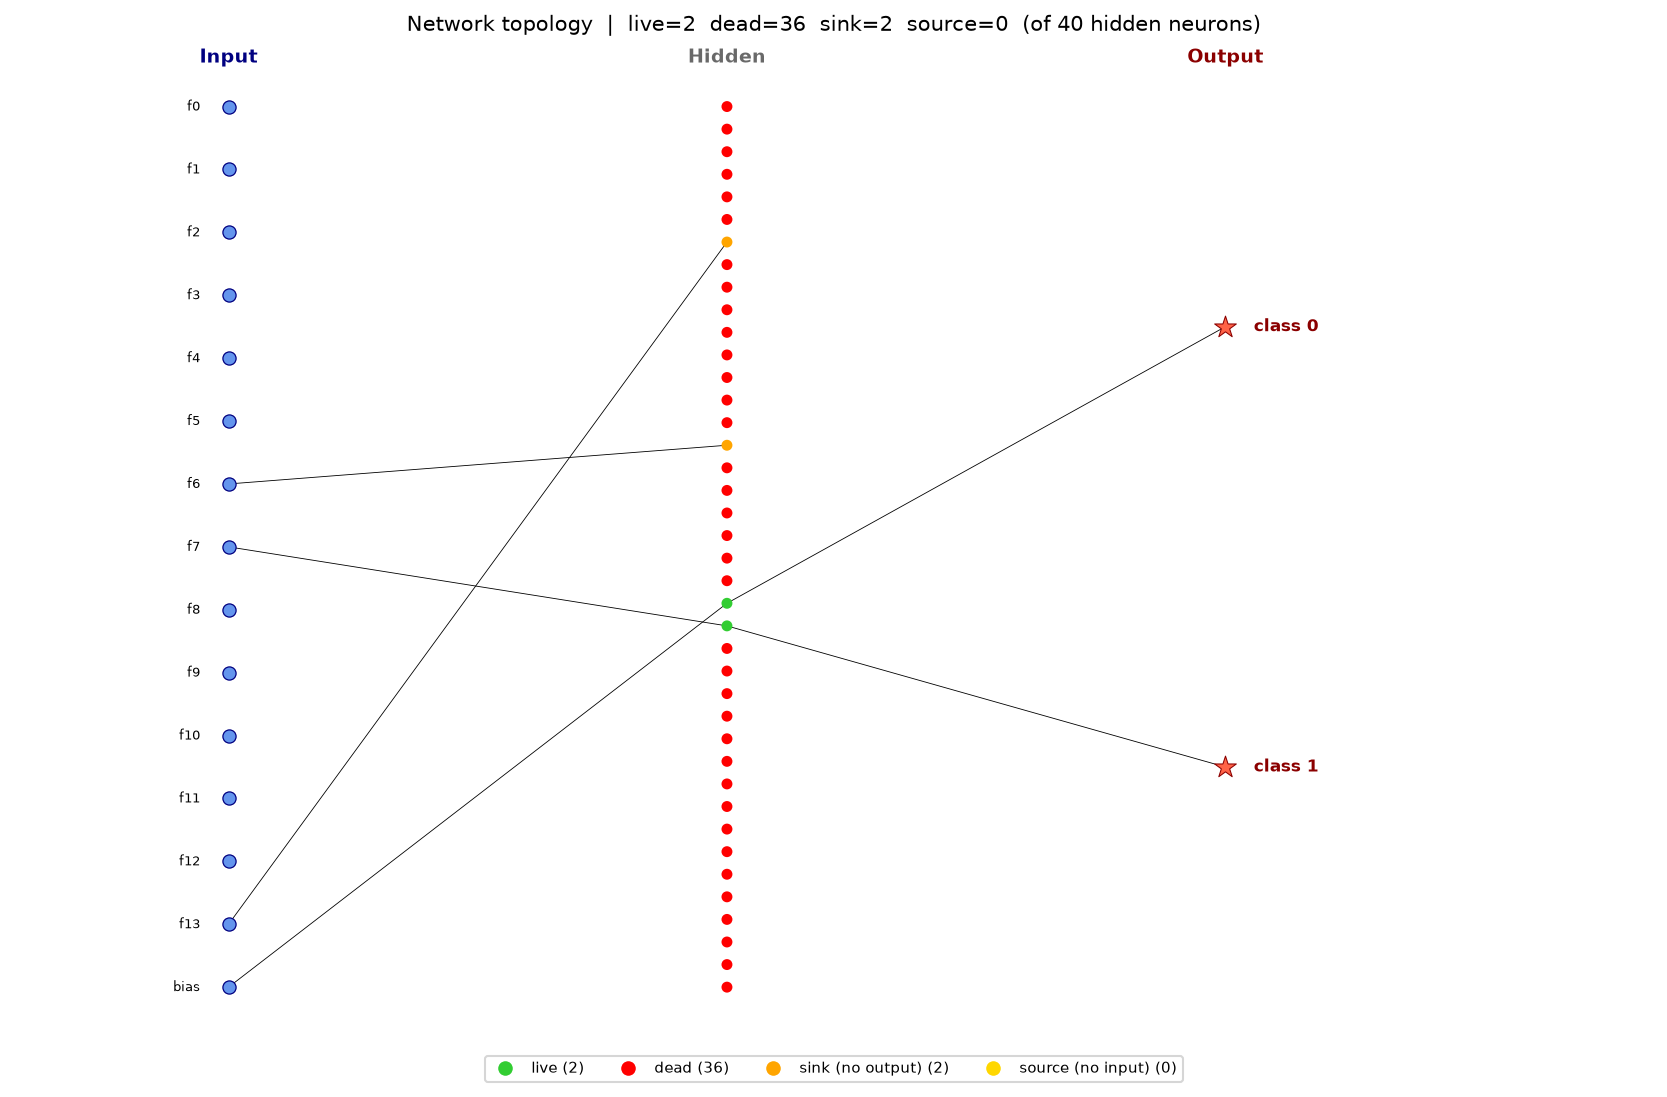
\includegraphics[width=\textwidth]{images/conectividad_ds1_moeackf.png}
    \caption{ds1-MOEA-CKF (corrida 3). Fila 1 de la Tabla~\ref{tab:conectividad-combo}.}
    \label{fig:conectividad-ds1-ckf}
\end{subfigure}
\hfill
\begin{subfigure}[b]{0.31\textwidth}
    \centering
    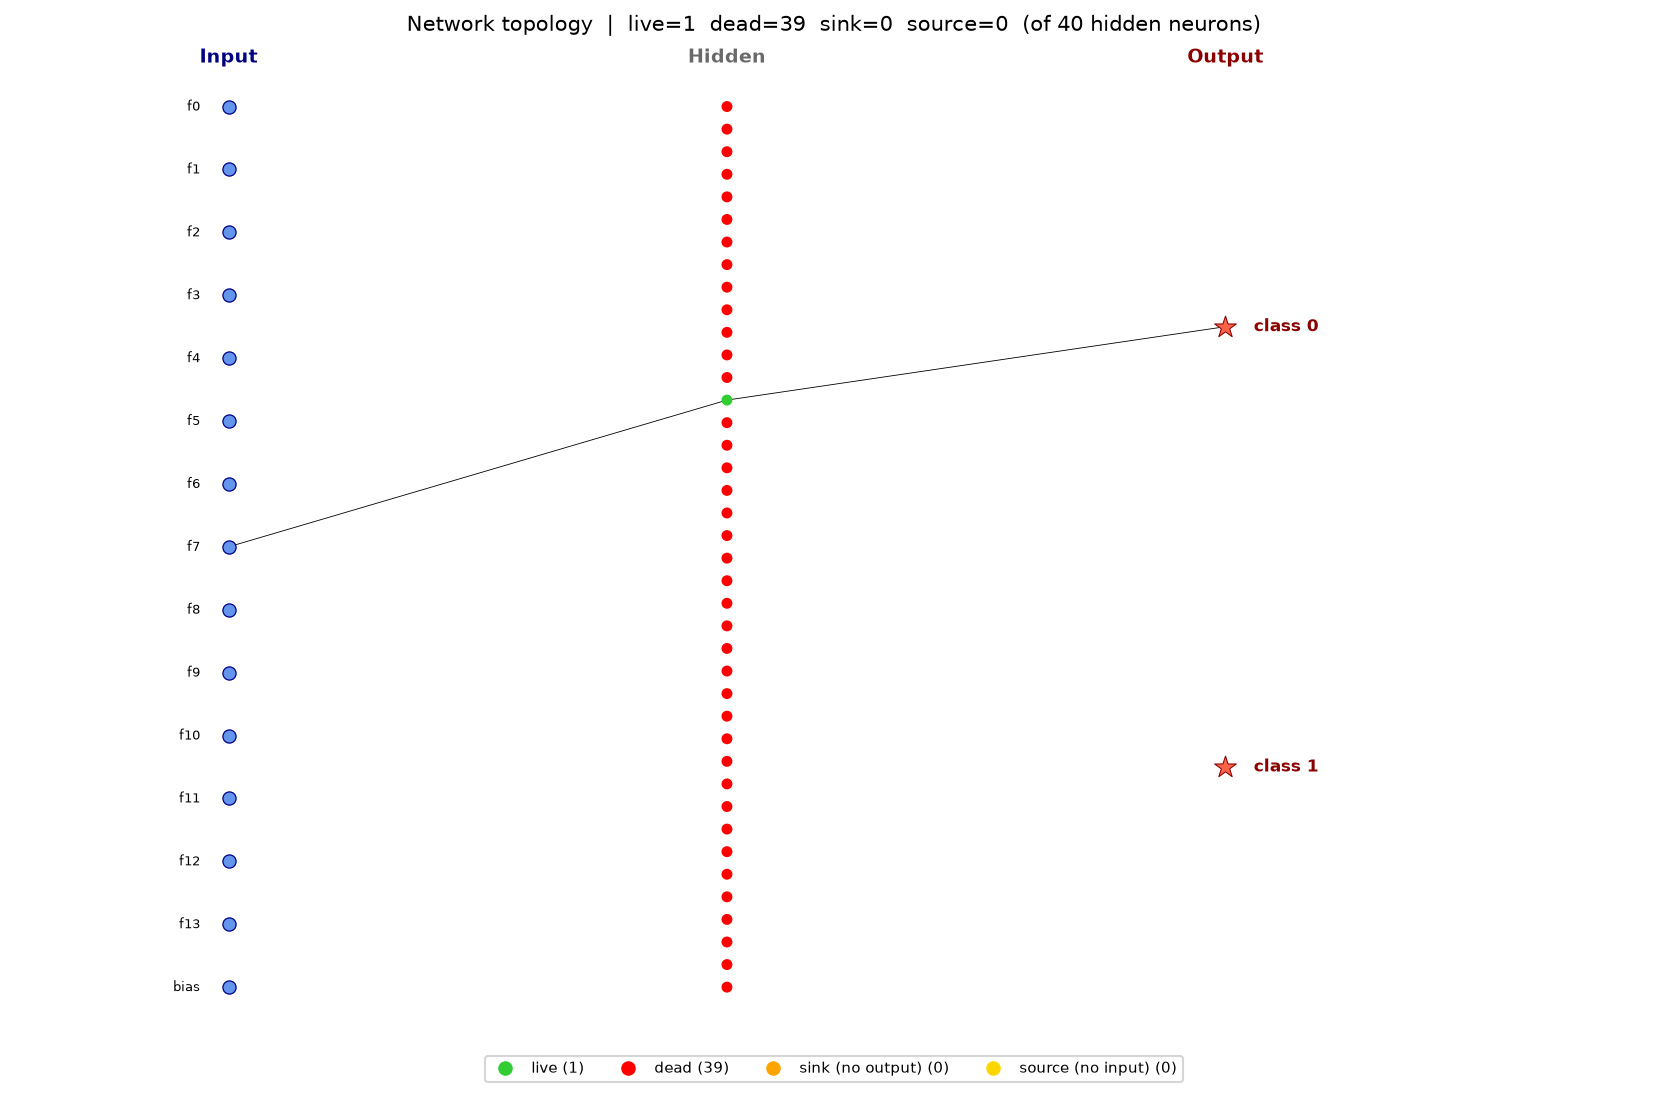
\includegraphics[width=\textwidth]{images/conectividad_ds1_snsgaii.png}
    \caption{ds1-S-NSGA-II (corrida 0). Fila 2 de la Tabla~\ref{tab:conectividad-combo}.}
    \label{fig:conectividad-ds1-nsga}
\end{subfigure}
\hfill
\begin{subfigure}[b]{0.31\textwidth}
    \centering
    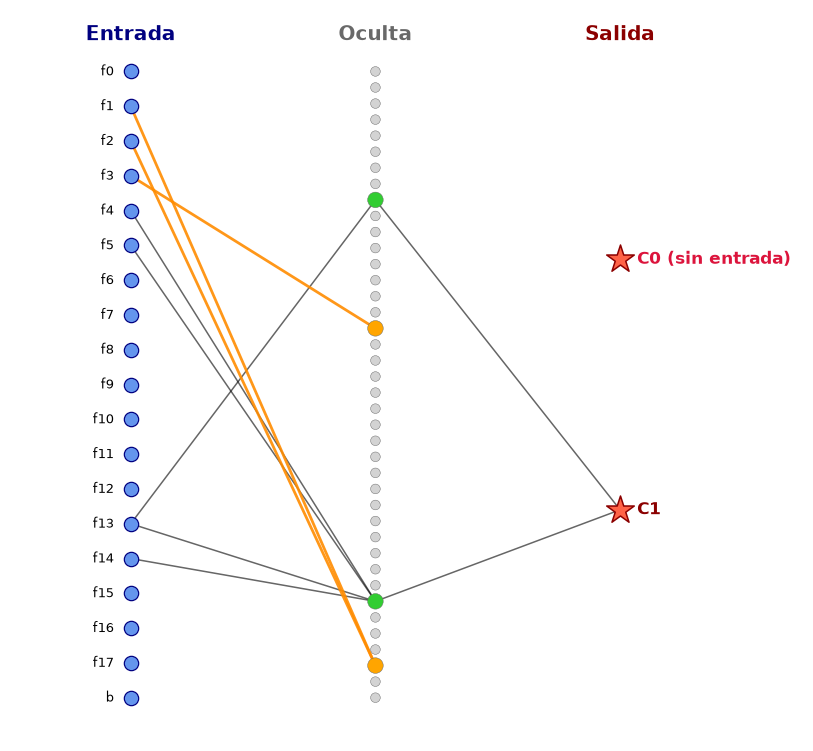
\includegraphics[width=\textwidth]{images/conectividad_ds2_moeackf.png}
    \caption{ds2-MOEA-CKF (corrida 24). Fila 3 de la Tabla~\ref{tab:conectividad-combo}.}
    \label{fig:conectividad-ds2-ckf}
\end{subfigure}

\par\vspace{0.4cm}

% Fila 2
\begin{subfigure}[b]{0.31\textwidth}
    \centering
    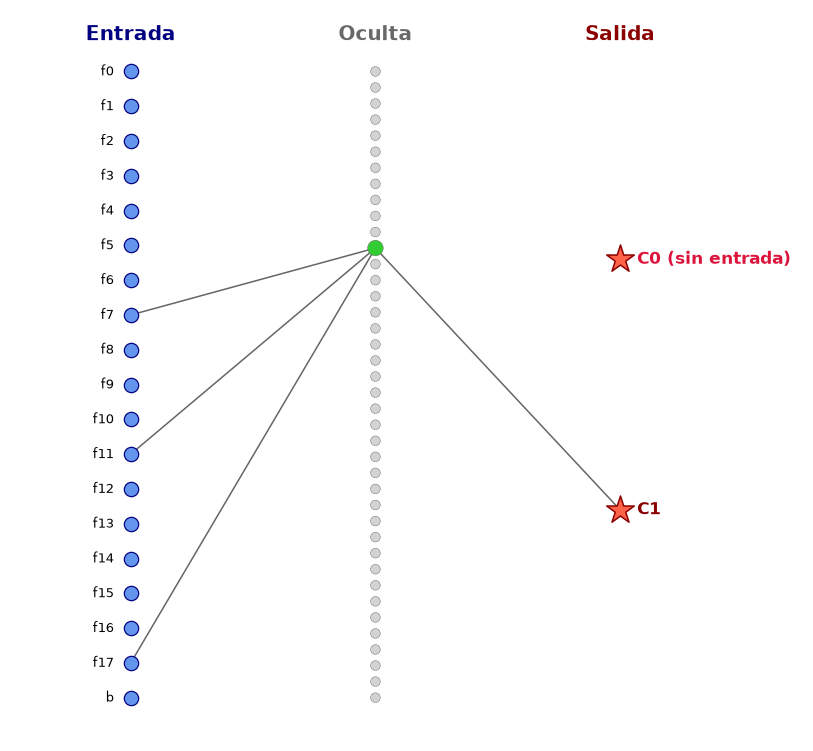
\includegraphics[width=\textwidth]{images/conectividad_ds2_snsgaii.png}
    \caption{ds2-S-NSGA-II (corrida 0). Fila 4 de la Tabla~\ref{tab:conectividad-combo}.}
    \label{fig:conectividad-ds2-nsga}
\end{subfigure}
\hfill
\begin{subfigure}[b]{0.31\textwidth}
    \centering
    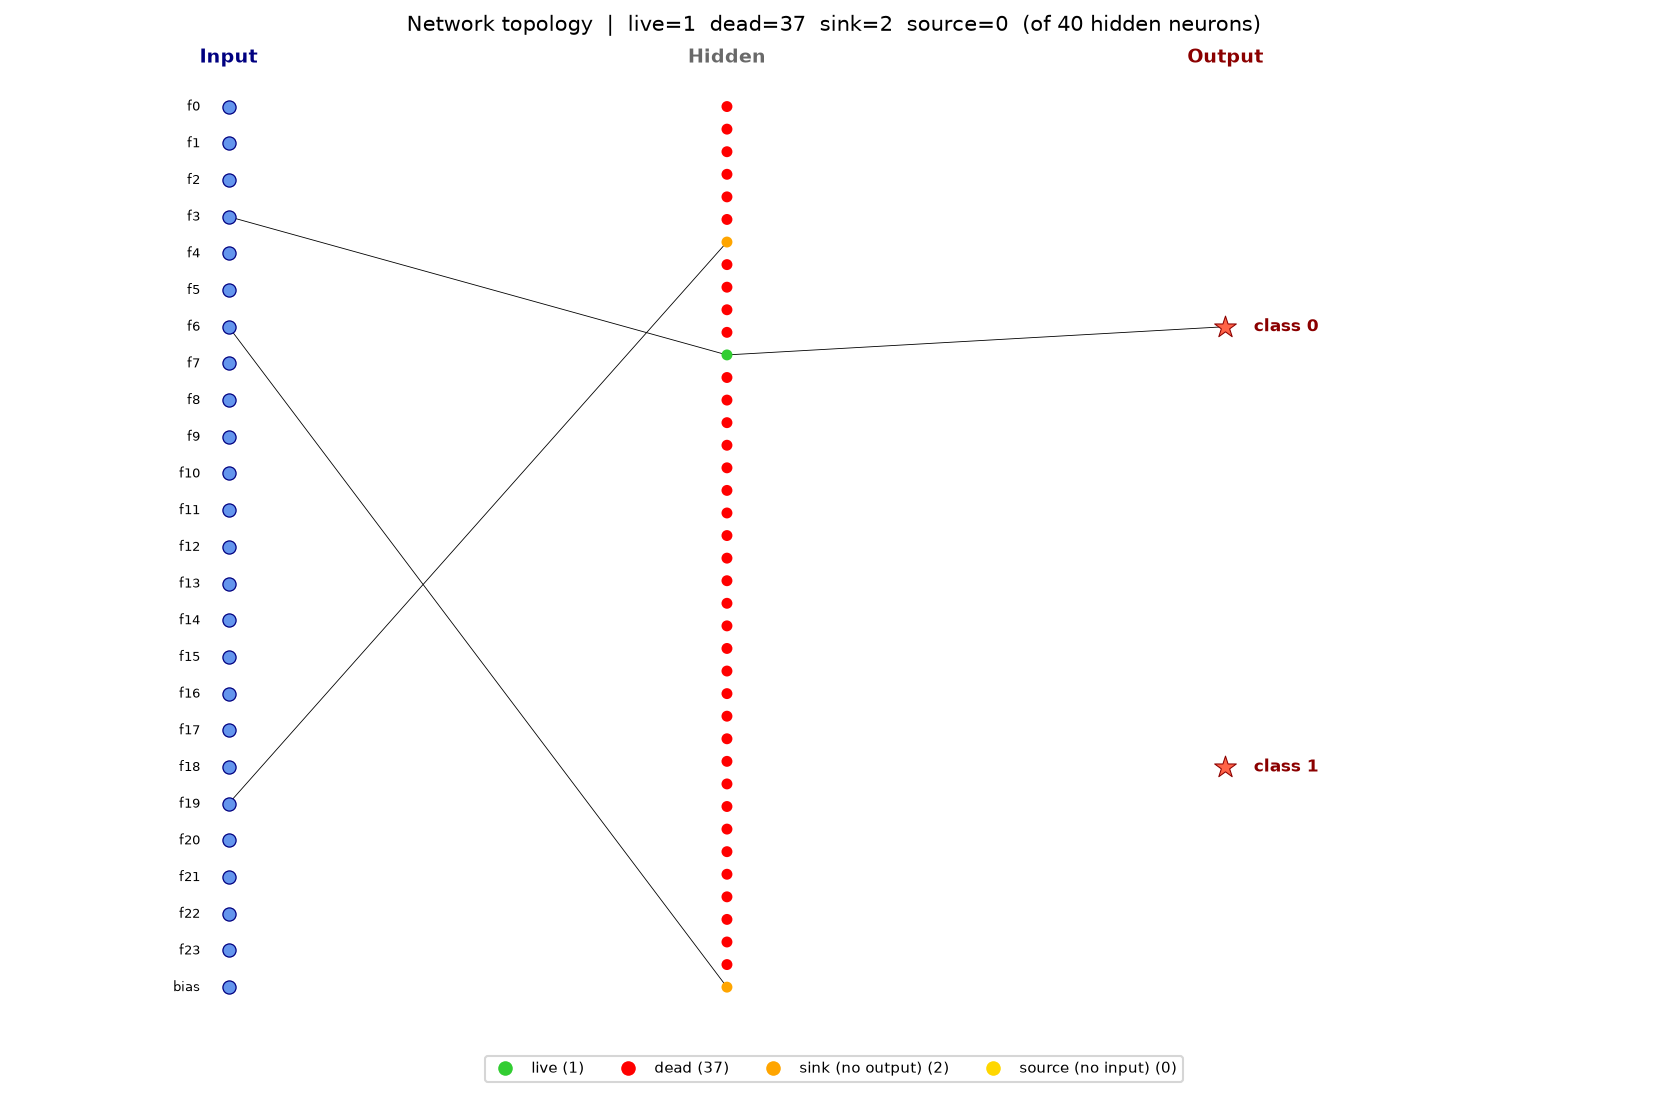
\includegraphics[width=\textwidth]{images/conectividad_ds3_moeackf.png}
    \caption{ds3-MOEA-CKF (corrida 20). Fila 5 de la Tabla~\ref{tab:conectividad-combo}.}
    \label{fig:conectividad-ds3-ckf}
\end{subfigure}
\hfill
\begin{subfigure}[b]{0.31\textwidth}
    \centering
    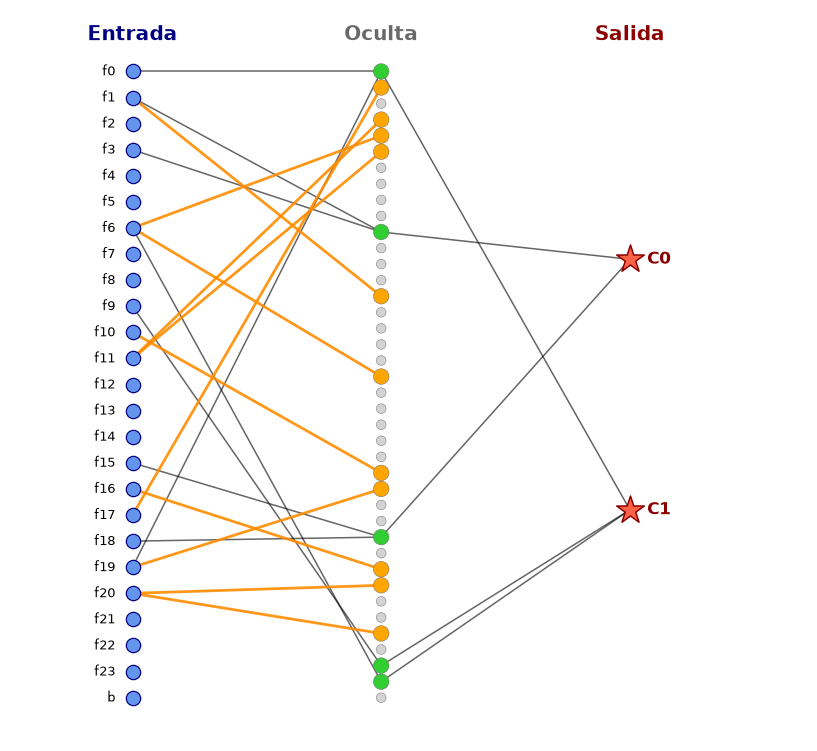
\includegraphics[width=\textwidth]{images/conectividad_ds3_snsgaii.png}
    \caption{ds3-S-NSGA-II (corrida 5). Fila 6 de la Tabla~\ref{tab:conectividad-combo}.}
    \label{fig:conectividad-ds3-nsga}
\end{subfigure}

\caption{Solución de mejor exactitud de una corrida representativa por combinación de dataset y algoritmo, \texttt{ds1}-\texttt{ds3} (\texttt{ds4} en el Anexo~A). Neuronas ocultas: vivas (verde), muertas (roja), sumidero (naranjo) y fuente (amarillo); estrellas rojas: neuronas de salida.}
\label{fig:conectividad-ejemplo}

\end{figure}
    \chapter{Discusión}

\section{Búsqueda de hiperparámetros}

El HV medio alcanzado por las mejores configuraciones depende principalmente de la dificultad del problema de clasificación y no de la dimensionalidad de entrada (aproximadamente 0.93 en \texttt{ds2}, 0.87 en \texttt{ds1}, 0.81 en \texttt{ds4} y 0.75 en \texttt{ds3}, sin relación monótona con el número de atributos), algo esperable dado que el HV combina simultáneamente exactitud y complejidad estructural. El análisis de importancia de hiperparámetros muestra que la escala de pesos (\texttt{wScale}) es sistemáticamente el hiperparámetro más influyente en tres de los cuatro estudios, coherente con su papel de amplificador necesario para que las conexiones codificadas entre [0,1] generen disparos efectivos en la red; las excepciones son \texttt{ds2}, dominado por la variable \texttt{architecture}, y \texttt{ds4}, donde la importancia se reparte entre varios hiperparámetros sin que ninguno domine, en un espacio de mayor dimensionalidad. Bajo un mismo presupuesto de búsqueda, MOEA-CKF y S-NSGA-II alcanzan HV prácticamente equivalentes en la configuración ganadora: en tres de los cuatro datasets (\texttt{ds1}, \texttt{ds3} y \texttt{ds4}) S-NSGA-II obtiene un HV medio ligeramente superior, con diferencias entre 0.002 y 0.016, mientras que en \texttt{ds2} la relación se invierte levemente a favor de MOEA-CKF, con una diferencia de apenas 0.0003; esto sugiere que, bajo el mismo presupuesto, ambos SMOEA podrían alcanzar HV comparables, aunque esta lectura se basa en el mejor \emph{trial} de un único estudio y se contrasta con mayor rigor estadístico en el Estudio 1. Estos resultados justifican tratar \texttt{architecture}, \texttt{wScale} y los límites de esparsidad como hiperparámetros externos del pipeline y sustentan las configuraciones utilizadas en la fase de comparación de algoritmos.

\section{Comparación de algoritmos}
\subsection{Estudio 1: Comparación de algoritmos en SNN}
\label{sec:discusion-estudio1}

\paragraph{Hipervolumen}

En hipervolumen (HV), S-NSGA-II obtiene una ventaja estadísticamente significativa en dos de los cuatro datasets (\texttt{ds1}, \texttt{ds3}), MOEA-CKF en uno (\texttt{ds4}), y en el restante (\texttt{ds2}) no se observa diferencia significativa. La magnitud de esta ventaja varía sustancialmente entre datasets: es más marcada en el de mayor dimensionalidad, \texttt{ds4} —donde además se invierte a favor de MOEA-CKF—, y es prácticamente inexistente en \texttt{ds2} (18 características), donde ambos algoritmos convergen a una región estrecha y muy alta del espacio de soluciones (diferencia mediana de solo 0.00016 entre medianas, con márgenes mínimos en las corridas donde gana S-NSGA-II y márgenes mayores en las pocas donde gana MOEA-CKF). Estos patrones son consistentes, aunque no concluyentes con solo cuatro puntos de datos, con la hipótesis de que S-NSGA-II rinde mejor en problemas de menor dimensionalidad (14 y 24 características) y MOEA-CKF en el de mayor dimensionalidad (60 características). Adicionalmente, en tres de los cuatro datasets (\texttt{ds1}, \texttt{ds2}, \texttt{ds3}) MOEA-CKF muestra menor varianza entre corridas que S-NSGA-II, incluso cuando pierde en mediana: tiende a ser más consistente y predecible entre ejecuciones, una propiedad relevante si el criterio de evaluación valora la reproducibilidad además del desempeño puntual.

\paragraph{Frentes de Pareto}

El patrón de complejidad-error observado en los frentes explica en gran medida las diferencias de HV descritas arriba: en los datasets donde gana S-NSGA-II (\texttt{ds1}, \texttt{ds3}), sus redes de mejor accuracy son sistemáticamente más densas y más exactas que las de MOEA-CKF, mientras que en \texttt{ds4}, donde gana MOEA-CKF, los roles se invierten y es este último quien produce redes más densas y más precisas. La cobertura mutua de los frentes combinados (C-metric) refuerza esta lectura: es relativamente pareja en \texttt{ds2} y \texttt{ds3} (en torno a 0.50/0.50 y 0.31/0.33) y marcadamente asimétrica en \texttt{ds4} (0.86/0.14 a favor de MOEA-CKF), de modo que el dataset con la ventaja de HV más contundente es también el de mayor dominancia punto a punto.

Sin embargo, HV y dominancia punto a punto no siempre coinciden: en \texttt{ds1}, pese a tener menos puntos en su frente combinado, el frente de MOEA-CKF domina en mayor proporción al de S-NSGA-II que al revés (55.6\% frente a 16.7\%), lo que indica que la ventaja de HV de S-NSGA-II proviene de cubrir una región más amplia del espacio de soluciones —en particular la banda de mayor complejidad, donde concentra la mayoría de sus puntos— y no de que cada solución individual sea mejor que su contraparte. Un mecanismo relacionado aparece en \texttt{ds3}, donde S-NSGA-II traduce el incremento de complejidad estructural en una reducción más sostenida del error a partir de cierto umbral, lo que explica que su frente combinado sea sustancialmente más grande y contribuye a su ventaja de HV. En \texttt{ds2}, en cambio, S-NSGA-II parece especializarse en soluciones muy esparsas con buenos resultados, mientras que MOEA-CKF explora una región más amplia sin obtener una ganancia proporcional, lo cual es coherente con que el HV no distinga a los algoritmos en ese dataset.

Dos limitaciones metodológicas condicionan esta lectura. Primero, el análisis de frentes se apoya en la solución de menor error de entrenamiento de cada corrida como sustituto de la accuracy de test, ya que el 100\% de las corridas archivadas usan arquitecturas de dos salidas (WTA) y no es posible medir la generalización de forma directa; se trata de una limitación estructural, no de un dato pendiente de calcular, y el análisis complejidad-error de todo el frente es el sustituto disponible. Segundo, el C-metric sobre los frentes combinados debe interpretarse como una magnitud aproximada y no como una proporción de alta precisión: tras deduplicar y filtrar soluciones no dominadas, estos frentes quedan reducidos a entre 4 y 14 puntos, lo que limita la resolución de la métrica en conjuntos tan pequeños.

\paragraph{Convergencia}

En los tres datasets donde existe una diferencia clara de HV (\texttt{ds1}, \texttt{ds3}, \texttt{ds4}), el algoritmo con menor HV final converge sistemáticamente más rápido a su propio techo, mientras que el de mayor HV final asciende más lentamente hacia uno más alto: MOEA-CKF llega antes a un techo más bajo en \texttt{ds1} y \texttt{ds3} ($\sim4.3\times$ más rápido en \texttt{ds1}), mientras que en \texttt{ds4} es S-NSGA-II quien se estabiliza antes en un nivel inferior y MOEA-CKF quien tarda $\sim2.4\times$ más en alcanzar el suyo, más alto, sin llegar a estabilizarse del todo dentro del presupuesto de evaluaciones. Un \textit{plateau} rápido en un techo bajo frente a un ascenso lento hacia un techo alto parece ser, entonces, un balance recurrente en este estudio, y no el ruido de una corrida aislada. En \texttt{ds2}, la ausencia de una diferencia relevante de HV se refleja también en la convergencia: la población inicial ya alcanza el 90\% del HV final para ambos algoritmos, por lo que la velocidad de convergencia mide más bien qué tan rápido se estabiliza la búsqueda que una carrera real de optimización sobre un problema comparativamente saturado.

Una limitación transversal a este análisis es que el eje de evaluaciones (FE) de las curvas y umbrales de velocidad es una aproximación por interpolación lineal dentro de cada corrida: no se registra el FE por fila sino solo la \texttt{generation}, que no es directamente comparable entre algoritmos porque MOEA-CKF consume más FE por generación que S-NSGA-II.

\subsection{Estudio 2: Plataforma SNN (C++) vs.\ ANN (MATLAB)}
\label{sec:discusion-estudio2}

Es el hallazgo más uniforme de todo el análisis: la implementación ANN original de PlatEMO/MATLAB supera a la SNN en HV y exactitud en las ocho combinaciones de dataset y algoritmo evaluadas, siempre de forma significativa tras corrección. La brecha de exactitud es menor en \texttt{ds1} y mayor en \texttt{ds4} para S-NSGA-II. La brecha de complejidad muestra, además, un patrón dependiente del algoritmo que se repite entre datasets: para S-NSGA-II, las redes ANN de mejor exactitud tienden a ser casi completamente densas frente a redes SNN mucho más esparsas (particularmente marcado en \texttt{ds2} y \texttt{ds3}), mientras que para MOEA-CKF esta brecha es sistemáticamente más moderada. La única excepción a este patrón ocurre en \texttt{ds4}, donde es la red SNN de MOEA-CKF la que resulta más densa que la ANN, la única anomalía de complejidad entre las ocho combinaciones plataforma-algoritmo del estudio. En conjunto, estos resultados sugieren que la SNN podría favorecer soluciones más esparsas que su contraparte ANN para una parte importante de las combinaciones algoritmo-dataset, un patrón dependiente del algoritmo que podría merecer investigación aparte.

MATLAB/PlatEMO original y la migración a C++ difieren en más que el modelo de neurona, ya que también difieren en la implementación y en el generador de números aleatorios. Por ello, los resultados de esta comparación deben leerse como evidencia de que la implementación ANN concreta supera consistentemente a la implementación SNN concreta evaluada aquí, y no como una conclusión general sobre la neurona de disparo frente a una neurona de tasa.

\subsection{Otros resultados}
\label{sec:discusion-otros}

El efecto del remuestreo sobre el HV final es heterogéneo entre datasets y algoritmos, sin que se identifique una regla simple. Mejora el HV de forma clara y con efecto grande en ambos algoritmos en \texttt{ds1} y \texttt{ds2} —este último con el menor costo relativo de tiempo de los cuatro datasets ($\times4.8$--$4.9$, frente a $\times5$--$15$ en el resto)—, pero produce resultados mixtos en \texttt{ds3} y \texttt{ds4}: en \texttt{ds3} solo mejora a MOEA-CKF, mientras que en S-NSGA-II no hay efecto significativo ($p=0.066$), con la dirección del tamaño de efecto incluso sugiriendo que la evaluación normal iguala o supera al remuestreo más seguido que a la inversa; en \texttt{ds4} el patrón se invierte y es solo S-NSGA-II quien mejora significativamente. El costo de tiempo del remuestreo, en cambio, es siempre sustancial (entre $\times4.8$ y $\times15.1$) independientemente de si el HV mejora o no, lo que deja como pregunta abierta si existe alguna interacción entre el remuestreo y los mecanismos específicos de cada algoritmo que explique esta heterogeneidad.

En tiempo de cómputo, S-NSGA-II es significativamente más rápido que MOEA-CKF en los cuatro datasets, con efecto grande y menor variabilidad entre corridas en todos los casos. La brecha, sin embargo, crece marcadamente con la dimensionalidad del problema: de aproximadamente $6$--$10\%$ en \texttt{ds1}--\texttt{ds3} (14--24 características) a cerca de $2.4\times$ en \texttt{ds4} (60 características, sin una sola excepción en las 15 corridas pareadas), donde MOEA-CKF resulta además el más lento y variable. Este patrón es consistente con que el mecanismo de fusión de conocimiento entre escalas de MOEA-CKF (SVD, análisis de dispersión) consume más FE por generación y escala peor con la dimensionalidad que los operadores más simples de S-NSGA-II.

Estas comparaciones de tiempo solo son válidas dentro del conjunto experimental temporal, ejecutado con hiperparámetros compartidos entre ambos algoritmos; los conjuntos experimentales normal y de remuestreo no permiten una comparación válida en tiempo de ejecución debido al paralelismo y los hilos no controlados entre tandas de ejecución, por lo que sus conclusiones de tiempo no deben mezclarse con las conclusiones de calidad (HV) del resto del análisis, que sí emplea hiperparámetros afinados.

\section{Conectividad de las redes}
\label{sec:discusion-conectividad-v2}

Los dos indicadores de la Sección~\ref{sec:conectividad} —clases de salida desconectadas y conexiones inútiles— responden a mecanismos distintos y conviene discutirlos por separado, aunque ambos comparten una misma raíz: ninguno de los operadores de dispersión de MOEACKF ni de S-NSGA-II tiene noción alguna de a qué neurona o a qué salida pertenece cada sinapsis, y ninguno de los dos objetivos de la optimización ($f_1$, complejidad; $f_2$, error de entrenamiento) penaliza directamente una sinapsis activa que no forma parte de ningún camino completo entre la entrada y la salida.

\subsection{Clases de salida desconectadas: desbalance de clases}

La asimetría por clase ya señalada en el análisis de resultados —en \texttt{ds2} es siempre la clase 0 la que pierde su conexión, en \texttt{ds3} es siempre la clase 1— coincide exactamente con la clase minoritaria de cada dataset: en \texttt{ds2} (Climate) la clase 0 representa apenas 46 de 540 instancias (8.5\%); en \texttt{ds3} (German) la clase minoritaria representa 300 de 1000 (30\%). En \texttt{ds1} (Australian, clase 0/clase 1: 55.5\%/44.5\%) y \texttt{ds4} (Sonar, 53.4\%/46.6\%), donde ambas clases están razonablemente balanceadas, el porcentaje de redes con una salida desconectada es nulo o casi nulo (0\% en tres de las cuatro combinaciones, 6.5\% en la restante). Esto es consistente con que, al no distinguir los operadores de dispersión entre clases al apagar pesos, basta con que $f_2$ (el error de entrenamiento) recompense predecir siempre la clase mayoritaria —una estrategia que en \texttt{ds2} ya alcanza 91.5\% de exactitud sin necesitar ninguna conexión hacia la clase minoritaria— para que la búsqueda converja hacia soluciones que sacrifican por completo la conectividad de esa clase, sin que el objetivo de exactitud lo impida.

La excepción parcial es \texttt{ds3}$\times$SNSGAII, con 0\% de salidas desconectadas pese al mismo desbalance 70/30 que en \texttt{ds3}$\times$MOEACKF produce 80.6\%. La diferencia es coherente con el diseño de cada operador: el operador de mutación de dispersión de S-NSGA-II muta un nivel de dispersión objetivo por individuo y apaga o reactiva pesos al azar hasta alcanzarlo, mientras que MOEACKF construye su máscara inicial activando un número aleatorio $k \in [1, D]$ de variables mediante selección por torneo sesgada por aptitud, sin ninguna garantía de que ese conjunto —que puede ser tan pequeño como una sola sinapsis de las $D$ totales— toque la neurona de salida de la clase minoritaria. Con un espacio de decisión de cientos o miles de variables, es más fácil que un sorteo casi puntual dependa del azar de la clase minoritaria que un ajuste incremental de densidad la deje completamente fuera, aunque esta lectura es una asociación entre el mecanismo del operador y el patrón observado, no una prueba directa sobre el código en ejecución.

\subsection{Conexiones inútiles: asimetría estructural y presión de poda débil}

El porcentaje de conexiones inútiles no aparece asociado con el desbalance de clases sino con la dimensionalidad de entrada: promediando ambos algoritmos por dataset (y excluyendo \texttt{ds2}$\times$SNSGAII por la razón que se explica más abajo), el porcentaje sube de 31.5\% en \texttt{ds1} (14 características) a 54.3\% en \texttt{ds3} (24 características) y 57.3\% en \texttt{ds4} (60 características). Esta tendencia es consistente con una explicación estructural propia de la codificación: cada neurona oculta tiene $n_F+1$ posiciones de entrada posibles (una por característica más el sesgo) pero solo $n_O=2$ posiciones de salida posibles, de modo que, ante cualquier mecanismo de activación de pesos sin conciencia de la estructura del grafo, la probabilidad de que una neurona reciba al menos una entrada activa crece con $n_F$ mucho más rápido que la probabilidad de que además tenga una salida activa —fija en solo dos posiciones—. Cuantas más características tiene el dataset, más fácil es entonces que una neurona termine con entrada real pero sin salida (sumidero) que con ambas (viva), lo que aumenta la fracción de sinapsis activas atrapadas en caminos incompletos. Esta lectura es razonable con solo cuatro datasets y ocho combinaciones, y no se contrastó de forma independiente del nivel de dispersión de cada solución.

\texttt{ds2}$\times$SNSGAII es la excepción que confirma esa lectura por la vía opuesta: su solución de mejor exactitud alcanza 92.1\% de accuracy con solo el 0.32\% de las 840 sinapsis activas y una única neurona oculta viva. Con tan pocas sinapsis activas en total, no queda margen combinatorio para que aparezcan neuronas parcialmente conectadas, y el 0\% de conexiones inútiles es entonces un efecto secundario de la extrema dispersión y no evidencia de una red mejor estructurada que el resto.

A esta asimetría estructural se suma una segunda causa, de naturaleza algorítmica: ninguno de los dos objetivos premia explícitamente eliminar una conexión inútil. Retirar una sinapsis que llega a una neurona sumidero (o que sale de una neurona fuente) reduce $f_1$ sin alterar $f_2$ en absoluto, de modo que la solución resultante domina estrictamente a la original y en teoría debería reemplazarla en el frente. En la práctica, esa poda solo ocurre si algún operador de variación llega a generar exactamente esa vecina —con esa sinapsis puntual desactivada y ninguna otra— dentro del presupuesto de evaluaciones disponible, algo cada vez menos probable a medida que $D$ crece (de 680 en \texttt{ds1} a 2520 en \texttt{ds4}) y que ninguno de los operadores dirige la búsqueda hacia esa vecina en particular. La diferencia entre algoritmos observada en la Tabla~\ref{tab:conectividad-algo} (49.5\% en MOEACKF frente a 32.7\% en S-NSGA-II) es consistente con esta lectura: la máscara de MOEACKF activa posiciones sueltas del vector de decisión sin agrupación alguna, mientras que la máscara de S-NSGA-II opera en franjas contiguas que —dado que la codificación agrupa las entradas de cada neurona oculta en un bloque contiguo del vector— tienden a activar o desactivar el bloque completo de una neurona en conjunto, produciendo con algo más de frecuencia neuronas enteramente vivas o enteramente muertas en vez de parcialmente conectadas.

\subsection{Implicancia práctica}

Ambos fenómenos afectan directamente a la red que se desplegaría en la práctica: en la Tabla~\ref{tab:conectividad-algo}, poco más de un tercio de las soluciones de mejor exactitud de MOEACKF y poco más de un cuarto de las de S-NSGA-II son incapaces de predecir una de las dos clases sin importar la entrada, y en promedio entre un tercio y la mitad de las sinapsis activas de esas soluciones no contribuye a ninguna predicción. Ninguno de los dos indicadores se corrige evaluando de mejor manera la red resultante, sino interviniendo en los operadores que deciden qué sinapsis permanecen activas: una inicialización o un operador de reparación que garanticen al menos un camino activo hacia cada clase de salida atacarían directamente el primer problema, y una poda estructural —que retire sinapsis pertenecientes a neuronas sumidero o fuente sin costo en $f_2$— atacaría el segundo; ninguna de las dos intervenciones fue implementada ni evaluada en el marco de esta tesis.

    \chapter{Conclusiones}\label{cap:conclusiones}

En este capítulo se evalúa el cumplimiento de cada uno de los objetivos específicos planteados en la Sección~\ref{sec:objetivos-especificos}, a la luz de los resultados presentados en el Capítulo~\ref{chapter:resultados} y de la discusión asociada. Cada objetivo se clasifica como \textbf{cumplido}, cuando la tarea se realizó satisfactoriamente; \textbf{cumplido parcialmente}, cuando se realizó pero persisten limitaciones relevantes; o \textbf{no cumplido}, cuando la tarea no pudo completarse.

El primer objetivo, seleccionar al menos un algoritmo evolutivo esparso, multiobjetivo y a gran escala, \textbf{se cumplió}. A partir de la taxonomía de SMOEAs esparsos de \cite{Shao2025_SMOEA} y de un proceso de preselección y selección final basado en criterios explícitos (cobertura de \textit{Real World NN training}, disponibilidad de código en PlatEMO y viabilidad de tiempos de ejecución), se identificaron y seleccionaron dos algoritmos, MOEA-CKF y S-NSGA-II, superando el mínimo de uno exigido por el objetivo. Ambos quedaron efectivamente aplicados al entrenamiento de SNN en las cuatro tareas de clasificación consideradas.

El segundo objetivo, seleccionar un framework de simulación SNN mediante análisis comparativo de ANNarchy, NEST, Brian2 y alternativas en C++, \textbf{se cumple parcialmente}. La selección final de \textit{snn-simulator} está respaldada por evidencia cuantitativa sólida: separación estadística completa ($U=0$, $p\approx3.0\times10^{-11}$) frente a ANNarchy y NEST en tiempo de evaluación, construcción de red en microsegundos y capacidad de evaluación batch paralela exclusiva. Sin embargo, de los frameworks mencionados en el objetivo, Brian2 solo fue descartado mediante análisis cualitativo de literatura, sin ser sometido al mismo benchmark cuantitativo aplicado a ANNarchy y NEST, por lo que la comparación empírica quedó acotada a tres de las cuatro alternativas propuestas.

El tercer objetivo, implementar un algoritmo evolutivo que optimice simultáneamente topología y pesos sinápticos para mejorar el equilibrio entre precisión y esparsidad, \textbf{se cumple parcialmente}. Se migraron e integraron exitosamente MOEA-CKF y S-NSGA-II en C++ junto al simulador Izhikevich, con una codificación de individuos que optimiza simultáneamente topología (mediante pesos nulos) y valores sinápticos, validada con 33 pruebas unitarias del simulador y produciendo frentes de Pareto error-complejidad en las cuatro tareas. No obstante, el análisis de conectividad (Sección~\ref{sec:discusion-conectividad-v2}) muestra que ninguno de los operadores de dispersión de ambos algoritmos tiene noción de la topología de la red: entre 26.6\% y 35.5\% de las mejores soluciones quedan con al menos una clase de salida sin ninguna conexión activa, y entre un tercio y la mitad de las sinapsis activas de esas soluciones no pertenece a ningún camino completo entrada-salida. El equilibrio buscado entre precisión y esparsidad se logra a nivel de los objetivos agregados, pero no garantiza redes funcionalmente coherentes a nivel estructural.

El cuarto objetivo, evaluar el desempeño del algoritmo en tareas de clasificación para verificar su capacidad de generalización y convergencia en al menos tres datasets, \textbf{se cumple parcialmente}. El algoritmo se validó experimentalmente en cuatro datasets (superando el mínimo exigido), con 31 corridas pareadas por semilla y análisis estadístico de hipervolumen, frentes de Pareto y velocidad de convergencia para cada combinación algoritmo-dataset. La convergencia quedó ampliamente caracterizada: se identificaron patrones consistentes de \textit{plateau} rápido en techos bajos frente a ascensos lentos hacia techos más altos. La capacidad de generalización, en cambio, no pudo verificarse de forma directa: el 100\% de las corridas archivadas usa arquitecturas de dos salidas (WTA), lo que impidió calcular una accuracy de test independiente, y el análisis debió sustituirla por el error de entrenamiento de la solución archivada como aproximación indirecta.

El quinto objetivo, comparar el enfoque evolutivo en SNN frente a modelos ANN equivalentes mediante Hipervolumen, \textbf{se cumplió}. Se realizó la comparación exigida contrastando la implementación SNN (C++) contra la implementación ANN original de PlatEMO/MATLAB en las ocho combinaciones de algoritmo y dataset. El resultado fue el hallazgo más uniforme de toda la investigación: la ANN superó a la SNN en HV y exactitud en las ocho combinaciones, siempre de forma significativa tras corrección estadística, mientras que en complejidad estructural la ventaja dependió del algoritmo, siendo la SNN consistentemente más esparsa que la ANN bajo S-NSGA-II y con una brecha más moderada bajo MOEA-CKF. Estas ventajas y desventajas quedaron identificadas con suficiente evidencia estadística, con la salvedad reconocida de que la comparación involucra además diferencias de implementación y generador de números aleatorios entre plataformas, por lo que sus conclusiones se limitan a las implementaciones concretas evaluadas y no a una comparación general entre neuronas de disparo y de tasa.

En conjunto, los cinco objetivos específicos se abordaron y ninguno quedó sin resolver, lo que permite sostener que el objetivo general, evaluar un algoritmo evolutivo de optimización esparsa multiobjetivo a gran escala para SNN, se cumple de manera parcial. El proyecto entregó una plataforma funcional en C++ capaz de optimizar simultáneamente precisión y esparsidad, validada estadísticamente en cuatro datasets y comparada rigurosamente contra su contraparte en ANN, pero dos limitaciones transversales condicionan una evaluación completamente satisfactoria: por un lado, la ANN de referencia superó a la SNN en las ocho combinaciones evaluadas, por lo que la eficiencia estructural de las SNN no se tradujo en una ventaja de desempeño; por otro, ni MOEA-CKF ni S-NSGA-II incorporan mecanismos conscientes de la topología de la red, de modo que una fracción relevante de las soluciones más precisas resulta estructuralmente incoherente (clases de salida inalcanzables o sinapsis sin función). Estas limitaciones no invalidan la propuesta, pero delimitan con precisión las direcciones de trabajo futuro: mecanismos de reparación o poda estructural conscientes de la topología, y una exploración más profunda de por qué la ventaja de esparsidad de las SNN no logró compensar su déficit de exactitud frente a la ANN.

    % \include{caps/resultados-comparacion}

	% ----------------------------------------------------------
	% ----------- TERCERA PARTE --------------------------------
	% ### Bibliografía de este documento ###
	% La opción heading la coloca en la tabla de contenidos
	\printbibliography[heading=bibintoc]
	
	% Alternativa de apéndices
	\appendix
	% \include{appendix/01-addendum}

	% Alternativa de anexos
	\annex
	% Por un bug del kernel de LaTeX (cf. el paquete appendix), si el primer
	% anexo está en un archivo aparte, debe ser incluido con \input, en lugar
	% de \include
	% Puede que lo logre arreglar en una futura versión de este template...
	% Idealmente :'v
	\chapter{Más cosas}

\begin{table}[htbp]
\centering
\small
\caption{Taxonomía de SMOEAs. Adaptado de \cite{Shao2025_SMOEA}.}
\label{tab:taxonomia-smoea}
% Ajusta los anchos aquí: 3.5cm para la 1ra columna, 3.2cm para la 2da, 5.5cm para la 3ra
\begin{tabular}{|C{3.5cm}|C{3.2cm}|C{5.5cm}|}
\hline
\textbf{Categoría} & \textbf{Subcategoría} & \textbf{Métodos específicos} \\
\hline
\multirow{10}{3.5cm}{\centering 1. MOEAs basados en nuevos operadores de variación}
 & \multirow{5}{3.2cm}{\centering 1.1 Volteo de variables} & Volteo estático de variables \\
 & & Volteo dinámico de variables \\
 & & Volteo híbrido de variables \\
 & & Volteo adaptativo de variables \\
 & & Volteo robusto de variables \\
\cline{2-3}
 & \multirow{2}{3.2cm}{\centering 1.2 Optimización convexa} & Operador disperso convexo \\
 & & Operador de truncamiento disperso \\
\cline{2-3}
 & \multirow{3}{3.2cm}{\centering 1.3 Operador novedoso} & Muestreo de población dispersa \\
 & & Operador adaptativo \\
 & & Población múltiple \\
\hline
\multirow{5}{3.5cm}{\centering 2. MOEAs basados en reducción de dimensionalidad}
 & \multirow{3}{3.2cm}{\centering 2.1 Redes neuronales} & Red neuronal no supervisada \\
 & & Aprendizaje por refuerzo profundo \\
 & & Perceptrón multicapa \\
\cline{2-3}
 & 2.2 Minería de patrones & --- \\
\cline{2-3}
 & 2.3 Interacción biniveles & --- \\
\hline
\multirow{6}{3.5cm}{\centering 3. MOEAs basados en agrupación de variables de decisión}
 & \multirow{3}{3.2cm}{\centering 3.1 Agrupación uniforme} & Agrupación aleatoria \\
 & & Agrupación dinámica \\
 & & Agrupación de granularidad múltiple \\
\cline{2-3}
 & \multirow{3}{3.2cm}{\centering 3.2 Agrupación no uniforme} & Agrupación rápida \\
 & & Agrupación no uniforme \\
 & & Agrupación adaptativa \\
\hline
\end{tabular}
\end{table}


\begin{table}
\centering
\small
\caption{Fidelidad de la migración a C++ de los operadores genéticos respecto de su implementación original en PlatEMO/MATLAB.}
\label{tab:fidelidad_algoritmos}
\begin{tabular}{p{5cm}p{2cm}p{6cm}}
\hline
\textbf{Componente} & \textbf{Fidelidad} & \textbf{Notas} \\
\hline
\texttt{vssps} --- inicialización stripe & Alta & La lógica de franjas fue traducida fielmente respecto de la implementación original. \\
\texttt{ssbx} --- sparse SBX & Alta & Se implementó correctamente el manejo de posiciones \textit{zero/nonzero} y los intercambios aleatorios en casos de desajuste (\textit{mismatches}). \\
\texttt{spm} --- sparse PM & Alta & Se implementó correctamente la mutación tanto de los valores como del nivel de esparsidad. \\
\texttt{sm2target} & Alta & El comportamiento de este componente se mantuvo fiel al original. \\
\texttt{EnvironmentalSelection \_NSGA2} & Alta & La traducción resultó fiel al original, incorporando además la corrección del error de conversión \textit{inf} $\rightarrow$ \textit{int}. \\
\hline
\end{tabular}
\end{table}

%-------------------------------------
\section{Resultados selección de framework de simulación}

\begin{table}[htbp]
\centering
\small
\caption{Tiempo de evaluación de \textit{fitness} en milisegundos con \(K = 30\).}
\label{tab:framework-evals-res}
\begin{tabular}{llrrrl}
\toprule
Config & Framework & \(n\) & Media \(\pm\) DE (ms) & Mediana (ms) & $p<0.05$ \\
\midrule
ds1\_h10 & snn-simulator & 30 & 44.40 \(\pm\) 1.15   & 44.09 & sí \\
ds1\_h10 & ANNarchy      & 30 & 158.52 \(\pm\) 2.40  & 157.95 & no \\
ds1\_h10 & NEST          & 30 & 2475.41 \(\pm\) 1043.56 & 2418.16 & sí \\ \hline
ds1\_h20 & snn-simulator & 30 & 60.39 \(\pm\) 1.72   & 59.92 & sí \\
ds1\_h20 & ANNarchy      & 30 & 160.60 \(\pm\) 2.91  & 160.05 & no \\
ds1\_h20 & NEST          & 30 & 2601.42 \(\pm\) 1067.47 & 2547.92 & sí \\ \hline
ds4\_h10 & snn-simulator & 30 & 39.15 \(\pm\) 0.60   & 39.05 & no \\
ds4\_h10 & ANNarchy      & 30 & 77.62 \(\pm\) 0.53   & 77.52 & no \\
ds4\_h10 & NEST          & 30 & 1023.46 \(\pm\) 323.54 & 1019.55 & sí \\ \hline
ds4\_h20 & snn-simulator & 30 & 46.00 \(\pm\) 4.08   & 45.11 & no \\
ds4\_h20 & ANNarchy      & 30 & 77.95 \(\pm\) 1.67   & 77.52 & no \\
ds4\_h20 & NEST          & 30 & 1045.15 \(\pm\) 305.28 & 1046.18 & sí \\ \hline
ds3\_h10 & snn-simulator & 30 & 90.25 \(\pm\) 0.91   & 90.09 & no \\
ds3\_h10 & ANNarchy      & 30 & 254.58 \(\pm\) 2.97  & 255.19 & sí \\
ds3\_h10 & NEST          & 30 & 3841.14 \(\pm\) 1545.16 & 3922.09 & sí \\ \hline
ds3\_h20 & snn-simulator & 30 & 115.27 \(\pm\) 2.67  & 114.39 & no \\
ds3\_h20 & ANNarchy      & 30 & 257.45 \(\pm\) 3.37  & 257.13 & no \\
ds3\_h20 & NEST          & 30 & 3938.56 \(\pm\) 1489.22 & 4100.74 & sí \\
\bottomrule
\end{tabular}
\end{table}


En memoria, ANNarchy es el más liviano (\(\approx 4{.}6\,\mathrm{MB}\)), seguido por \textit{snn-simulator} (\(\approx 13{.}35\,\mathrm{MB}\)), mientras que NEST emplea entre 28{.}56 y 138{.}08 MB. Pruebas previas con $K=15$ que no se muestran aquí confirman que NEST acumula estado o memoria proporcionalmente al número de evaluaciones repetidas dentro de un mismo proceso, pasando de aproximadamente \( 66{.}6\,\mathrm{MB}\) a \( 137{.}7\,\mathrm{MB}\) en \texttt{ds3\_h10}, y de alrededor de \( 66{.}9\,\mathrm{MB}\) a \(\approx 138{.}1\,\mathrm{MB}\) en \texttt{ds3\_h20}.

\begin{table}[htbp]
\centering
\small
\caption{Tiempo de construcción y memoria pico por configuración y framework.}
\label{tab:framework-build-memory-res}
\begin{tabular}{llrr}
\toprule
Config & Framework & Construcción & Memoria pico \\
\midrule
ds1\_h10 & SNN-Simulator & 0.040 ms & 13.35 MB \\
ds1\_h10 & ANNarchy      & 773.39 ms (+ 9.79 s compilación Cython) & 4.63 MB \\
ds1\_h10 & NEST          & 3.04 ms  & 96.72 MB \\
ds1\_h20 & SNN-Simulator & 0.053 ms & 13.35 MB \\
ds1\_h20 & ANNarchy      & 762.32 ms (+ 9.69 s compilación) & 4.57 MB \\
ds1\_h20 & NEST          & 3.33 ms  & 97.11 MB \\
ds4\_h10 & SNN-Simulator & 0.072 ms & 13.35 MB \\
ds4\_h10 & ANNarchy      & 760.77 ms (+ 9.74 s compilación) & 4.71 MB \\
ds4\_h10 & NEST          & 5.21 ms  & 28.56 MB \\
ds4\_h20 & SNN-Simulator & 0.180 ms & 13.35 MB \\
ds4\_h20 & ANNarchy      & 768.38 ms (+ 9.69 s compilación) & 4.69 MB \\
ds4\_h20 & NEST          & 5.62 ms  & 29.01 MB \\
ds3\_h10 & SNN-Simulator & 0.037 ms & 13.35 MB \\
ds3\_h10 & ANNarchy      & 766.97 ms (+ 9.64 s compilación) & 4.59 MB \\
ds3\_h10 & NEST          & 3.51 ms  & 137.68 MB \\
ds3\_h20 & SNN-Simulator & 0.059 ms & 13.35 MB \\
ds3\_h20 & ANNarchy      & 764.19 ms (+ 9.82 s compilación) & 4.59 MB \\
ds3\_h20 & NEST          & 3.89 ms  & 138.08 MB \\
\bottomrule
\end{tabular}
\end{table}


\begin{table}[htbp]
\centering
\caption{Escalabilidad de \textit{snn-simulator} al evaluar una población de 100 individuos con diferentes números de hilos.}
\label{tab:framework-batch-res}
\small
\begin{tabular}{lrrrrr}
\toprule
Config & 1 hilo (s) & speedup 2 hilos & speedup 4 hilos & speedup 8 hilos & speedup 12 hilos \\
\midrule
ds1\_h10 & 4.43 &  1.54 (77.1\% ef.) &  2.43 (60.9\% ef.) &  4.46 (55.8\% ef.) &  5.20 (43.3\% ef.) \\
ds1\_h20 & 5.98 &  1.98 (98.9\% ef.) &  2.86 (71.6\% ef.) &  4.55 (56.9\% ef.) &  5.36 (44.6\% ef.) \\
ds4\_h10 & 3.95 &  1.99 (99.4\% ef.) &  2.87 (71.7\% ef.) &  4.44 (55.5\% ef.) &  5.22 (43.5\% ef.) \\
ds4\_h20 & 4.48 &  1.97 (98.6\% ef.) &  2.86 (71.4\% ef.) &  4.52 (56.5\% ef.) &  5.27 (43.9\% ef.) \\
ds3\_h10 & 9.15 &  1.99 (99.3\% ef.) &  2.87 (71.9\% ef.) &  4.52 (56.5\% ef.) &  5.13 (42.8\% ef.) \\
ds3\_h20 & 11.46 &  1.99 (99.6\% ef.) &  2.90 (72.4\% ef.) &  4.57 (57.1\% ef.) &  5.38 (44.8\% ef.) \\
\bottomrule
\end{tabular}
\end{table}
	\chapter{Pseudocódigo algoritmos evolutivos}\label{chap:anexo-pseudo}

\section{MOEA-CKF}\label{sec:pseudo-moeackf}
 
\begin{algorithm}[H]
\caption{Framework de MOEA/CKF}
\KwIn{$N$ (tamaño de población), $D$ (número de variables), $M$ (número de objetivos), $T$ (número de ciclos de muestreo)}
\KwOut{$P$ (población final)}
$pv \leftarrow \text{AnálisisPrevio}(D,T)$ \tcp*{Algoritmo 2}
$P \leftarrow \text{Inicialización}(N, pv)$\;
$\rho \leftarrow 0.5$ \tcp*{probabilidad de que un individuo entre a $P_1$}
\While{no se agoten las evaluaciones de función}{
    $[GSI, LSI, pv, Group, \eta] \leftarrow \text{AnálisisDeEsparsidad}(P, pv)$ \tcp*{Algoritmo 3}
    \tcp{Dividir la población}
    $P_1 \leftarrow \emptyset$, $P_2 \leftarrow \emptyset$\;
    \ForEach{$p \in P$}{
        \eIf{$rand < \rho$}{
            $P_1 \leftarrow P_1 \cup \{p\}$\;
        }{
            $P_2 \leftarrow P_2 \cup \{p\}$\;
        }
    }
    \tcp{Generar descendencia}
    $O_1 \leftarrow \text{Reproducción1}(P_1, Group, GSI, LSI, \eta)$ \tcp*{Algoritmo 4}
    $O_2 \leftarrow \text{Reproducción2}(P_2, Group)$ \tcp*{Algoritmo 5}
    $P \leftarrow P \cup O_1 \cup O_2$\;
    Eliminar soluciones duplicadas de $P$\;
    $P \leftarrow \text{SelecciónAmbiental}(P, N)$\;
}
\Return{$P$}
\end{algorithm}
 
\begin{algorithm}[H]
\caption{AnálisisPrevio$(D, T)$}
\KwIn{$D$ (número de variables de decisión), $T$ (número de ciclos de muestreo)}
\KwOut{$P$ (población inicializada), $pv$ (vector de conocimiento previo)}
$score \leftarrow$ vector de ceros $1\times D$\;
$pv \leftarrow$ vector de ceros $1\times D$\;
\For{$i = 1$ \KwTo $T$}{
    $XR \leftarrow$ matriz aleatoria $D\times D$\;
    $XB \leftarrow$ matriz identidad $D\times D$\;
    $Q \leftarrow$ población cuya $i$-ésima solución se genera con las $i$-ésimas filas de $XR$ y $XB$ según (1)\;
    $[F_1, F_2, \dots] \leftarrow$ ordenamiento no dominado sobre $Q$\;
    \For{$i = 1$ \KwTo $D$}{
        $score_i \leftarrow k$, tal que $Q_i \in F_k$ \tcp*{$Q_i$ denota la $i$-ésima solución de $Q$}
    }
    $pv = pv + score$\;
}
\Return{$pv$}
\end{algorithm}
 
\begin{algorithm}[H]
\caption{AnálisisDeEsparsidad$(P, pv)$}
\KwIn{$P$ (población actual), $pv$ (vector de conocimiento previo)}
\KwOut{$GSI$ (información de esparsidad global), $LSI$ (información de esparsidad local), $Group$ (agrupamiento por clustering), $pv$ (vector de conocimiento previo actualizado), $\eta$ (proporción de soluciones no dominadas en la población actual)}
$AllOne \leftarrow$ conjunto de variables que valen uno en el vector binario $\mathbf{xb}$ de todas las soluciones de $P$\;
$AllZero \leftarrow$ conjunto de variables que valen cero en $\mathbf{xb}$ de todas las soluciones de $P$\;
$GSI \leftarrow [AllOne, AllZero]$\;
$R \leftarrow$ todas las soluciones no dominadas de $P$\;
$allone \leftarrow$ conjunto de variables que valen uno en $\mathbf{xb}$ de todas las soluciones de $R$\;
$allzero \leftarrow$ conjunto de variables que valen cero en $\mathbf{xb}$ de todas las soluciones de $R$\;
$LSI \leftarrow [allone, allzero]$\;
$sv \leftarrow$ vector de ceros $1\times D$\;
$sv \leftarrow$ actualizar $sv$ según (3)\;
$\delta \leftarrow$ proporción de evaluaciones consumidas\;
$\eta \leftarrow |R|/|P|$\;
$pv \leftarrow$ actualizar $pv$ según (4)\;
\tcp{Particionar las variables de decisión en dos clusters}
$[S_1, S_2] \leftarrow$ aplicar $k$-means sobre $pv$ para clasificar las variables de decisión en dos clusters\;
\eIf{el valor medio de $pv$ en el cluster $S_1$ es menor que el de las variables en $S_2$}{
    $NSV \leftarrow S_1$; $SV \leftarrow S_2$\;
}{
    $NSV \leftarrow S_2$; $SV \leftarrow S_1$\;
}
$Group \leftarrow \{NSV, SV\}$\;
\Return{$(GSI, LSI, pv, Group, \eta)$}
\end{algorithm}
 
\begin{algorithm}[H]
\caption{Reproducción1$(P, Group, GSI, LSI, \eta)$}
\KwIn{$P$ (subpoblación), $Group$ (grupos de variables), $GSI$ (información de esparsidad global), $LSI$ (información de esparsidad local), $\eta$ (proporción de soluciones no dominadas en la población original)}
\KwOut{$O$ (descendencia)}
$PR \leftarrow$ matriz $|P|\times D$ con los vectores reales de todas las soluciones de $P$\;
$[u_1, u_2, \dots, u_D] \leftarrow$ usar PCA sobre $PR$ para calcular sus autovectores según sus autovalores en orden descendente\;
$[NSV, SV] \leftarrow Group$\;
$[AllOne, AllZero] \leftarrow GSI$\;
$NSV' \leftarrow$ eliminar de $NSV$ las dimensiones que están en $AllOne$ y $AllZero$\;
$K \leftarrow |AllOne| + |NSV'|$\;
$U_{reduce} \leftarrow [u_1, u_2, \dots, u_K]$ \tcp*{seleccionar componentes principales con parámetro $K$}
$[Front, CrowdDis] \leftarrow$ ordenamiento no dominado y cálculo de la distancia de aglomeración sobre $P$\;
$Q \leftarrow$ seleccionar $2\times|P|$ padres mediante torneo binario según el número de frente no dominado y $CrowdDis$ de las soluciones de $P$\;
$O \leftarrow \emptyset$ \tcp*{conjunto de descendencia}
\While{$Q \neq \emptyset$}{
    $[\mathbf{x}, \mathbf{y}] \leftarrow$ seleccionar aleatoriamente dos soluciones de $Q$\;
    $Q \leftarrow Q \setminus \{\mathbf{x}, \mathbf{y}\}$\;
    $\mathbf{ob} \leftarrow$ vector de ceros $1\times D$\;
    \eIf{$rand < \eta$}{
        $[Allone, Allzero] \leftarrow LSI$\;
    }{
        $[Allone, Allzero] \leftarrow GSI$\;
    }
    $NSV' \leftarrow$ eliminar de $NSV$ las dimensiones que están en $Allone$ y $Allzero$\;
    $SV' \leftarrow$ eliminar de $SV$ las dimensiones que están en $Allone$ y $Allzero$\;
    $\mathbf{ob}(NSV') \leftarrow \text{OperadoresBinarios}(\mathbf{xb}(NSV'), \mathbf{yb}(NSV'))$\;
    $\mathbf{ob}(SV') \leftarrow \text{OperadoresBinarios}(\mathbf{xb}(SV'), \mathbf{yb}(SV'))$\;
    $\mathbf{ob}(Allone) \leftarrow 1$\;
    $[\mathbf{xr}_{reduce}, \mathbf{yr}_{reduce}] \leftarrow \mathbf{xr}\cdot U_{reduce}$ y $\mathbf{yr}\cdot U_{reduce}$\;
    $\mathbf{or}_{reduce} \leftarrow$ aplicar SBX y PM sobre $\mathbf{xr}_{reduce}$ y $\mathbf{yr}_{reduce}$\;
    $\mathbf{or} \leftarrow \mathbf{or}_{reduce}\cdot U_{reduce}^{T}$\;
    $\mathbf{o} \leftarrow$ generar solución descendiente según (1) a partir de $\mathbf{ob}$ y $\mathbf{or}$\;
    $O \leftarrow O \cup \{\mathbf{o}\}$\;
}
\Return{$O$}
\end{algorithm}
 
\begin{algorithm}[H]
\caption{Reproducción2$(P, Group)$}
\KwIn{$P$ (subpoblación), $Group$ (grupos de variables)}
\KwOut{$O$ (población descendiente)}
$[Front, CrowdDis] \leftarrow$ ordenamiento no dominado y cálculo de la distancia de aglomeración sobre $P$\;
$Q \leftarrow$ seleccionar $2\times|P|$ padres mediante torneo binario según el número de frente no dominado y $CrowdDis$ de las soluciones de $P$\;
$[NSV, SV] \leftarrow Group$\;
$O \leftarrow \emptyset$\;
\While{$Q \neq \emptyset$}{
    $[\mathbf{x}, \mathbf{y}] \leftarrow$ seleccionar aleatoriamente dos soluciones de $Q$\;
    $Q \leftarrow Q \setminus \{\mathbf{x}, \mathbf{y}\}$\;
    $\mathbf{ob} \leftarrow$ vector de ceros $1\times D$\;
    $\mathbf{ob}(NSV) \leftarrow \text{OperadoresBinarios}(\mathbf{xb}(NSV), \mathbf{yb}(NSV))$\;
    $\mathbf{ob}(SV) \leftarrow \text{OperadoresBinarios}(\mathbf{xb}(SV), \mathbf{yb}(SV))$\;
    $\mathbf{or} \leftarrow$ vector de ceros $1\times D$\;
    $[nonzeros, zeros] \leftarrow \mathbf{ob}$\;
    $\mathbf{or}(nonzeros) \leftarrow$ aplicar SBX y PM sobre $\mathbf{xr}(nonzeros)$ y $\mathbf{yr}(nonzeros)$\;
    $\mathbf{or}(zeros) \leftarrow$ aplicar SBX y PM sobre $\mathbf{xr}(zeros)$ y $\mathbf{yr}(zeros)$\;
    $\mathbf{o} \leftarrow$ generar solución descendiente según (1) a partir de $\mathbf{ob}$ y $\mathbf{or}$\;
    $O \leftarrow O \cup \{\mathbf{o}\}$\;
}
\Return{$O$}
\end{algorithm}

\section{S-NSGA-II}\label{sec:pseudo-snsgaii}

\begin{algorithm}[H]
\caption{SSPS$(N, D, P_i, \mathbf{s})$}
\KwIn{$N$ (tamaño de población), $D$ (número de variables de decisión), $P_i$ (población muestreada por defecto), $\mathbf{s}$ (vector de esparsidad objetivo de la población)}
\KwOut{$P_s$ (población inicial)}
\tcp{--- DETERMINAR LOS CICLOS ---}
$\mathbf{w} \leftarrow$ determinar el ancho de las franjas para cada individuo multiplicando cada $s\in\mathbf{s}$ por $D$\;
$\mathbf{c} \leftarrow$ inicializar un conjunto vacío de ciclos\;
\tcp{Determinar el número de individuos por ciclo}
$cycleStart \leftarrow 1$ \tcp*{individuo actual}
\While{queden miembros de la población}{
    $cycleEnd \leftarrow cycleStart + 1$ \tcp*{individuo al final del ciclo}
    \tcp{¿Cuántas franjas caben en el ciclo actual?}
    \While{suma de anchos entre $cycleStart$ y $cycleEnd$ $< D$}{
        $cycleEnd$++ \tcp*{mover el final del ciclo un individuo más}
    }
    $\mathbf{c}$.append($\mathbf{w}[cycleStart:cycleEnd]$) \tcp*{agregar nuevo ciclo, o serie de anchos de franja}
    $cycleStart \leftarrow cycleEnd + 1$ \tcp*{ir al inicio del siguiente ciclo}
}
\tcp{--- DIBUJAR LAS FRANJAS ---}
$currentIndiv \leftarrow 1$ \tcp*{contador de individuos}
$M_s \leftarrow$ inicializar una máscara de esparsidad vacía\;
\ForEach{$currentCycle \in \mathbf{c}$}{
    $stripeGap \leftarrow$ determinar si existe un vacío en $currentCycle$ (ver Fig.~3)\;
    \eIf{es el último ciclo}{
        $currentCycle \leftarrow$ espaciar las franjas dejando vacíos entre ellas para llenar $stripeGap$\;
    }{
        $currentCycle \leftarrow$ ensanchar las franjas de $currentCycle$ para llenar $stripeGap$\;
    }
    \ForEach{$currentStripe \in currentCycle$}{
        $M_s[currentIndiv, currentStripe] \leftarrow 1$ \tcp*{``dibujar'' la franja}
        $currentIndiv$++\;
    }
}
$P_s \leftarrow P_i \circ M_s$\;
\Return{$P_s$}
\end{algorithm}
 
\begin{algorithm}[H]
\caption{S-SBX$(P_1, P_2, p_c, \eta_c)$}
\KwIn{$P_1$ (padres a cruzar con $P_2$), $P_2$ (padres a cruzar con $P_1$), $p_c$ (probabilidad de cruce), $\eta_c$ (índice de distribución de la PDF de cruce)}
\KwOut{$C_1$ (primer hijo de $P_1$ y $P_2$), $C_2$ (segundo hijo de $P_1$ y $P_2$)}
\tcp{--- SBX EN POSICIONES 0/0 Y $\neq$0/$\neq$0 ---}
$Mask_{n1} \leftarrow$ posiciones distintas de cero de $P_1$\;
$Mask_{z1} \leftarrow$ posiciones iguales a cero de $P_1$\;
$Mask_{n2} \leftarrow$ posiciones distintas de cero de $P_2$\;
$Mask_{z2} \leftarrow$ posiciones iguales a cero de $P_2$\;
\tcp{Posiciones que son ambas cero o ambas distintas de cero}
$Mask_m = (Mask_{n1} \wedge Mask_{n2}) \vee (Mask_{z1} \wedge Mask_{z2})$\;
\tcp{Ejecutar SBX en estas posiciones}
$C_1[Mask_m], C_2[Mask_m] \leftarrow \text{SBX}(P_1[Mask_m], P_2[Mask_m], p_c, \eta_c)$\;
\tcp{--- INTERCAMBIO ALEATORIO PARA EL RESTO DE VALORES ---}
$Mask_{\neg m} \leftarrow \neg Mask_m$\;
\tcp{El vector $v$ indica qué pares se intercambian}
$v \leftarrow \mathbf{0}_{1,|Mask_{\neg m}|}$\;
$v \leftarrow$ distribuir unos uniformemente en $v$ de modo que cada posición tenga 50\% de probabilidad de ser 1\;
\tcp{Intercambiar genes según $v$}
$C_1[Mask_{\neg m}], C_2[Mask_{\neg m}] \leftarrow$ intercambiar entre $P_1[Mask_{\neg m}]$ y $P_2[Mask_{\neg m}]$ según $v$\;
\Return{$C_1, C_2$}
\end{algorithm}
 
\begin{algorithm}[H]
\caption{S-PM$(P, p_m, \eta_m)$}
\KwIn{$P$ (población de entrada), $p_m$ (probabilidad de mutación), $\eta_m$ (índice de distribución de la PDF de mutación)}
\KwOut{$P_m$ (población mutada)}
$P_m \leftarrow P$\;
\tcp{--- MUTAR LOS VALORES DISTINTOS DE CERO CON PM ---}
$Mask_n \leftarrow$ posiciones de $P$ distintas de cero\;
$P_m[Mask_n] \leftarrow \text{PM}(P[Mask_n], p_m, \eta_m)$\;
\tcp{--- MUTAR LA ESPARSIDAD ---}
$\mathbf{s} \leftarrow$ calcular la esparsidad de cada individuo en $P$\;
$\mathbf{s}_m \leftarrow \text{PM}(\mathbf{s}, p_m, \eta_m)$\;
\ForEach{$i$-ésimo miembro de $P_m$}{
    \If{$s_{m_i} < s_i$}{
        $P_{m_i} \leftarrow$ cambiar suficientes valores no nulos a cero en $P_{m_i}$ para igualar $s_{m_i}$\;
    }
    \If{$s_{m_i} > s_i$}{
        $P_{m_i} \leftarrow$ cambiar suficientes ceros a valores no nulos plausibles en $P_{m_i}$ para igualar $s_{m_i}$\;
    }
}
\Return{$P_m$}
\end{algorithm}
	\chapter{Repositorios de código}\label{chap:anexo-repos}

El código fuente desarrollado para esta tesis se encuentra disponible públicamente, separado en los dos módulos descritos en el Capítulo \ref{cap:implementacion}: el simulador de SNN y el framework de algoritmos evolutivos.

\begin{description}
    \item[snn-simulator] Implementa el modelo de neurona de Izhikevich, la estructura de la red y los mecanismos de codificación y decodificación de espigas (ver Sección \ref{sec:simulador-snn}).\\
    \url{https://github.com/Don-Uldaricio/snn-simulator}

    \item[platemo-cpp] Contiene la migración a C++ de S-NSGA-II y MOEA-CKF desde PlatEMO, junto con la integración de ambos algoritmos con el simulador de SNN (ver Sección \ref{sec:algoritmos-evolutivos}).\\
    \url{https://github.com/Don-Uldaricio/platemo-cpp}
\end{description}

	
\end{document}